\documentclass[UTF8,zihao = -4]{ctexart}
\usepackage{pdfpages}
%%%%%%%%------------------------------------------------------------------------
%%%% 日常所用宏包

%% 控制页边距
\usepackage[papersize={370mm,260mm},top=2.cm, bottom=2cm, left=2.cm, right=2.cm,includefoot]{geometry}

%% 控制项目列表
\usepackage{enumerate}

%% 多栏显示
\usepackage{multicol}

%% hyperref宏包,生成可定位点击的超链接,并且会生成pdf书签
%\usepackage[%
%    pdfstartview=FitH,%
%    CJKbookmarks=true,%
%    bookmarks=true,%
%    bookmarksnumbered=true,%
%    bookmarksopen=true,%
%    colorlinks=true,%
%    citecolor=blue,%
%    linkcolor=blue,%
%    anchorcolor=green,%
%    urlcolor=blue%
%]{hyperref}

%% 控制标题
%\usepackage{titlesec}

%% 控制表格样式
%\usepackage{booktabs}

%% 控制目录
%\usepackage{titletoc}

%% 控制字体大小
%\usepackage{type1cm}

%% 首行缩进,用\noindent取消某段缩进
%\usepackage{indentfirst}

%% 支持彩色文本、底色、文本框等
\usepackage{color,xcolor}

%%%% 基本插图方法
%% 图形宏包
\usepackage{graphicx}

%% 多个图形并排,参加lnotes.pdf
\usepackage{subfig}

% \begin{figure}[htbp]               %% 控制插图位置
%   \setlength{\abovecaptionskip}{0pt}
%   \setlength{\belowcaptionskip}{10pt}
                                     %% 控制图形和上下文的距离
%   \centering                       %% 使图形居中显示
%   \includegraphics[width=0.8\textwidth]{CTeXLive2008.jpg}
                                     %% 控制图形显示宽度为0.8\textwidth
%   \caption{CTeXLive2008安装过程} \label{fig:CTeXLive2008}
                                     %% 图形题目和交叉引用标签
% \end{figure}
%%%% 基本插图方法结束

%%%% pgf/tikz绘图宏包设置
\usepackage{pgf,tikz}
\usetikzlibrary{shapes,automata,snakes,backgrounds,arrows}
\usetikzlibrary{mindmap}

%%%% fancyhdr设置页眉页脚
%% 页眉页脚宏包
\usepackage{fancyhdr}
\pagestyle{plain}

\usepackage{tabu}
\usepackage{multirow}
\usepackage{calc,marvosym,ifthen,fancybox,url,layout}

\newcolumntype{M}[1]{>{\zihao{-4} \centering\arraybackslash}m{#1}}
\newcolumntype{N}{@{}m{0pt}@{}}

\setlength{\parindent}{0pt}

\newcommand{\xn}[1]{\gdef\xnNR{#1}} %学年
\newcommand{\xq}[1]{\gdef\xqNR{#1}} %学期
\newcommand{\xb}[1]{\gdef\xbNR{#1}} %系部
\newcommand{\zy}[1]{\gdef\zyNR{#1}} %专业
\newcommand{\bj}[1]{\gdef\bjNR{#1}} %班级
\newcommand{\kc}[1]{\gdef\kcNR{#1}} %课程
\newcommand{\skzs}[1]{\gdef\skzsNR{#1}} %上课周数
\newcommand{\zxs}[1]{\gdef\zxsNR{#1}} %周学时

\newcommand{\jk}[1]{\gdef\jkNR{#1}} %讲课
\newcommand{\sy}[1]{\gdef\syNR{#1}} %实验
\newcommand{\lljk}[1]{\gdef\lljkNR{#1}} %理论讲课
\newcommand{\sx}[1]{\gdef\sxNR{#1}} %实训
\newcommand{\sxlljk}[1]{\gdef\sxlljkNR{#1}} %实习理论讲课
\newcommand{\scsx}[1]{\gdef\scsxNR{#1}} %生产实习
\newcommand{\kh}[1]{\gdef\khNR{#1}} %考核
\newcommand{\jd}[1]{\gdef\jdNR{#1}} %机动
\newcommand{\hj}[1]{\gdef\hjNR{#1}} %机动

\newcommand{\ywcks}[1]{\gdef\ywcksNR{#1}} %已完成课时
\newcommand{\ylks}[1]{\gdef\ylksNR{#1}} %余留课时
\newcommand{\khfs}[1]{\gdef\khfsNR{#1}} %考试方式
\newcommand{\jcmc}[1]{\gdef\jcmcNR{#1}} %教材名称

\newcommand{\ud}[2]{\underline{\makebox[#1]{\textbf{#2}}} }

\newcommand{\jhsy}{ %生成计划首页
\setlength{\columnsep}{50pt } 
\columnseprule=0.4pt \twocolumn

\begin{center}
	\begin{tabular}{M{15em}M{4cm}N}
		\parbox{12em}{ \linespread{0.2}\zihao{-4} \bf \heiti	
			\makebox[12em][s]{湖南九嶷职业技术学院}\\[0.1cm]
			\makebox[12em][s]{湖南潇湘技师学院}
		}
		&  \zihao{1} \heiti \makebox[4cm][s]{\rule{0pt}{0.9cm}授课计划}&\\
	\end{tabular}
	\vspace{0.8cm}
	
	\zihao{3} \bf  \underline{~~~\xnNR~~~} 学年  \underline{~~~\xqNR~~~}  学期
\end{center}

\begin{tabular}{Nllll}
	&系部:\underline{\makebox[8em]{\textbf{\xbNR}}}& 
	专业: \underline{\makebox[8em]{\textbf{\zyNR}}}&
	班级: \underline{\makebox[12em]{\textbf{\bjNR}}}& \\[2ex]
	&课程:\underline{\makebox[8em]{\textbf{\kcNR}}}&
	上课周数:\underline{\makebox[6em]{\textbf{\skzsNR}}} &
	周学时:  \underline{\makebox[11em]{\textbf{\zxsNR}}} & 
\end{tabular}
\vspace{1ex}

{\bf 本学期课时分配表}
\vspace{1ex}

%\hspace{-0.5em}
\begin{tabu}{|M{4em}|M{2.5em}|M{2.5em}|M{2.5em}|M{3em}|M{2.5em}|M{2.5em}|M{2.5em}|M{2.5em}|M{4em}|N}
	\hline 
	教学\linebreak 模式 & \multicolumn{2}{c|}{理论}& \multicolumn{2}{c|}{一体化} & \multicolumn{2}{c|}{实习}&  \multirow{2}{1em}{ 考\vspace{1cm} 核 }& \multirow{2}{1em}{ 机\vspace{1cm} 动 }  &
	\multirow{2}{1em}{  合\vspace{1cm} 计 } & \\[4.5ex]
	\cline{1-7} 
	教学\linebreak 形式& 讲\linebreak\linebreak 课 & 实\linebreak\linebreak  验 & 理\linebreak 论\linebreak 讲\linebreak 课& 实\linebreak\linebreak 训 & 理\linebreak 论\linebreak 讲\linebreak 课 & 生\linebreak 产\linebreak 实\linebreak 习 &&&&\\ [12ex]
	\hline 
	课时&\jkNR &\syNR &\lljkNR &\sxNR &\sxlljkNR &\scsxNR &\khNR&\jdNR &\hjNR & \\[7ex]
	\hline 
\end{tabu} 

~\vspace{3ex}

说明:与本课程无关教学模式的各项各打×
\vspace{0.5ex}

备注:~~
\begin{minipage}[t]{15cm}\vspace{-1.25em}
	\begin{enumerate}[1、\hspace{-5pt}]
		\item 本课程以前完成学时数:\underline{\makebox[23em]{\textbf{\ywcksNR}}}
		\item 本课程在以后学期尚余留时数:\underline{\makebox[20em]{\textbf{\ylksNR}}}        
		\item 本课程本学期列为考试(考查)课程:\underline{\makebox[17em]{\textbf{\khfsNR}}} 
		\item 本课程使用教材名称: \underline{\makebox[24em]{\textbf{\jcmcNR}}}
	\end{enumerate}
\end{minipage}
\vspace{1ex}

\setlength{\baselineskip}{1.5\baselineskip}
\makebox[5em][s]{任课教师}:\ud{10em}{}  \hspace{1em} 编写日期:\ud{5.5em}{}年\ud{3em}{}月\ud{3em}{}日\\
\makebox[5em][s]{教研室主任}:\ud{10em}{}  \hspace{1em} 编写日期:\ud{5.5em}{}年\ud{3em}{}月\ud{3em}{}日\\
\makebox[5em][s]{系主任}:\ud{10em}{}  \hspace{1em} 编写日期:\ud{5.5em}{}年\ud{3em}{}月\ud{3em}{}日\\
\makebox[5em][s]{教务处}:\ud{10em}{}  \hspace{1em} 编写日期:\ud{5.5em}{}年\ud{3em}{}月\ud{3em}{}日\\
\makebox[5em][s]{分管领导}:\ud{10em}{}  \hspace{1em} 编写日期:\ud{5.5em}{}年\ud{3em}{}月\ud{3em}{}日\\
\pagebreak
}

\newcolumntype{L}[1]{>{\zihao{-4} \arraybackslash}m{#1}}
 \newenvironment{jxjhb}{
	\newpage \noindent
	
	
	\begin{center}
		\begin{tabu}{M{12em}M{6cm}N}
		\parbox{12em}{\linespread{0.2}
				\zihao{-4} \bf \heiti	\makebox[12em][s]{湖南九嶷职业技术学院}\\[0.1cm]
				\makebox[12em][s]{湖南潇湘技师学院}
			}
			&  \zihao{1} \heiti \makebox[8cm][s]{\rule{0pt}{0.9cm}教师学期授课计划}&\\
		\end{tabu}
	\end{center}
	
	\begin{tabu}{|>{\centering}M{1.5cm}|L{6cm}|L{9cm}|>{\centering}M{4cm}|>{\centering}M{5cm}|>{\centering}M{2cm}|>{\centering}M{2.cm}|N}
		\hline 
		周次&\centering 授课章节内容摘要&\centering 教学 要求& 教具及实验\par 实习材料& 作业及参考材料& 教学\par 时数& 备注& \\[6ex] \hline }
	{ 
	\end{tabu} 
	\vspace{4ex}
}

\newcommand{\shqz}{ 
	
	\hspace{10cm}  {\zihao{3}    任课教师:\ud{8em}{} \hfill 教研室主任:\ud{8em}{}  \hfill 系主任: \ud{8em}{}  \hfill}} %审核签字


%% 首页格式
%\input{data/shouye}

%\numberwithin{table}{section}
%\numberwithin{figure}{section}
%\usepackage[labelsep=quad]{caption}
%\makeatletter
%\def\fnum@figure#1{\figurename\nobreakspace\thefigure\hspace{1em}}%去掉图后面的冒号并加空白空1em
%\def\fnum@table#1{\tablename\nobreakspace\thetable\hspace{1em}}%去掉表后面的冒号并加空白1em
%\makeatother

%%%% 导言区结束
%%%%%%%%------------------------------------------------------------------------

%%%%%%%%------------------------------------------------------------------------

%%%% 公共信息
\jsxm{高星} %教师姓名
\jyszr{高星}	%教研室主任
\jc{《数控机床编程与操作(数控铣床加工中心分册)》沈建峰}%教材
\cks{《加工中心编程与操作》刘加孝主编}%参考书
\skbc{16级大专数控班}%授课班次
\biaoti{理论}%标题头

%%%% 正文部分
\begin{document}
\addcontentsline{toc}{section}{封面-前}
\begin{titlepage}
	
\begin{center}
{ \zihao{1} \bf
\makebox[10cm][s]{湖南九嶷职业技术学院}  \\
\makebox[10cm][s]{湖南潇湘技师学院} \\ }
\vfill 
{ \zihao{1} \fangsong  \fontsize{46pt}{80pt}\selectfont
   教\par 案\par 本\par }
\par
\vfill \vfill \zihao{4} \setlength{\baselineskip}{1cm}  \bf  
 授课教师:\underline{ \makebox[5cm]{ \jsxmNR}}\par
 授课课程:\underline{ \makebox[5cm]{ 数铣编程与操作}}\par
授课班级:\underline{ \makebox[5cm]{ \skbcNR}} 
\vfill
{\bf 二O一七 }——{\bf 二O一八}~~学年\hspace{0.5cm} 第~{\bf 一}~学期
\end{center}
\vfill

\end{titlepage}

%\newpage
%%%%% 导言区
%% 设定纸张大小为A4, 基本字体大小为12pt, 文章题目单独为一页, 
%% 文档类型为article
%\documentclass[12pt]{article}
%
%%% en_preamble包含基本的宏包配置
%%%%%%%%%------------------------------------------------------------------------
%%%% 日常所用宏包

%% 控制页边距
\usepackage[papersize={370mm,260mm},top=2.cm, bottom=2cm, left=2.cm, right=2.cm,includefoot]{geometry}

%% 控制项目列表
\usepackage{enumerate}

%% 多栏显示
\usepackage{multicol}

%% hyperref宏包,生成可定位点击的超链接,并且会生成pdf书签
%\usepackage[%
%    pdfstartview=FitH,%
%    CJKbookmarks=true,%
%    bookmarks=true,%
%    bookmarksnumbered=true,%
%    bookmarksopen=true,%
%    colorlinks=true,%
%    citecolor=blue,%
%    linkcolor=blue,%
%    anchorcolor=green,%
%    urlcolor=blue%
%]{hyperref}

%% 控制标题
%\usepackage{titlesec}

%% 控制表格样式
%\usepackage{booktabs}

%% 控制目录
%\usepackage{titletoc}

%% 控制字体大小
%\usepackage{type1cm}

%% 首行缩进,用\noindent取消某段缩进
%\usepackage{indentfirst}

%% 支持彩色文本、底色、文本框等
\usepackage{color,xcolor}

%%%% 基本插图方法
%% 图形宏包
\usepackage{graphicx}

%% 多个图形并排,参加lnotes.pdf
\usepackage{subfig}

% \begin{figure}[htbp]               %% 控制插图位置
%   \setlength{\abovecaptionskip}{0pt}
%   \setlength{\belowcaptionskip}{10pt}
                                     %% 控制图形和上下文的距离
%   \centering                       %% 使图形居中显示
%   \includegraphics[width=0.8\textwidth]{CTeXLive2008.jpg}
                                     %% 控制图形显示宽度为0.8\textwidth
%   \caption{CTeXLive2008安装过程} \label{fig:CTeXLive2008}
                                     %% 图形题目和交叉引用标签
% \end{figure}
%%%% 基本插图方法结束

%%%% pgf/tikz绘图宏包设置
\usepackage{pgf,tikz}
\usetikzlibrary{shapes,automata,snakes,backgrounds,arrows}
\usetikzlibrary{mindmap}

%%%% fancyhdr设置页眉页脚
%% 页眉页脚宏包
\usepackage{fancyhdr}
\pagestyle{plain}

\usepackage{tabu}
\usepackage{multirow}
\usepackage{calc,marvosym,ifthen,fancybox,url,layout}

\newcolumntype{M}[1]{>{\zihao{-4} \centering\arraybackslash}m{#1}}
\newcolumntype{N}{@{}m{0pt}@{}}

\setlength{\parindent}{0pt}

\newcommand{\xn}[1]{\gdef\xnNR{#1}} %学年
\newcommand{\xq}[1]{\gdef\xqNR{#1}} %学期
\newcommand{\xb}[1]{\gdef\xbNR{#1}} %系部
\newcommand{\zy}[1]{\gdef\zyNR{#1}} %专业
\newcommand{\bj}[1]{\gdef\bjNR{#1}} %班级
\newcommand{\kc}[1]{\gdef\kcNR{#1}} %课程
\newcommand{\skzs}[1]{\gdef\skzsNR{#1}} %上课周数
\newcommand{\zxs}[1]{\gdef\zxsNR{#1}} %周学时

\newcommand{\jk}[1]{\gdef\jkNR{#1}} %讲课
\newcommand{\sy}[1]{\gdef\syNR{#1}} %实验
\newcommand{\lljk}[1]{\gdef\lljkNR{#1}} %理论讲课
\newcommand{\sx}[1]{\gdef\sxNR{#1}} %实训
\newcommand{\sxlljk}[1]{\gdef\sxlljkNR{#1}} %实习理论讲课
\newcommand{\scsx}[1]{\gdef\scsxNR{#1}} %生产实习
\newcommand{\kh}[1]{\gdef\khNR{#1}} %考核
\newcommand{\jd}[1]{\gdef\jdNR{#1}} %机动
\newcommand{\hj}[1]{\gdef\hjNR{#1}} %机动

\newcommand{\ywcks}[1]{\gdef\ywcksNR{#1}} %已完成课时
\newcommand{\ylks}[1]{\gdef\ylksNR{#1}} %余留课时
\newcommand{\khfs}[1]{\gdef\khfsNR{#1}} %考试方式
\newcommand{\jcmc}[1]{\gdef\jcmcNR{#1}} %教材名称

\newcommand{\ud}[2]{\underline{\makebox[#1]{\textbf{#2}}} }

\newcommand{\jhsy}{ %生成计划首页
\setlength{\columnsep}{50pt } 
\columnseprule=0.4pt \twocolumn

\begin{center}
	\begin{tabular}{M{15em}M{4cm}N}
		\parbox{12em}{ \linespread{0.2}\zihao{-4} \bf \heiti	
			\makebox[12em][s]{湖南九嶷职业技术学院}\\[0.1cm]
			\makebox[12em][s]{湖南潇湘技师学院}
		}
		&  \zihao{1} \heiti \makebox[4cm][s]{\rule{0pt}{0.9cm}授课计划}&\\
	\end{tabular}
	\vspace{0.8cm}
	
	\zihao{3} \bf  \underline{~~~\xnNR~~~} 学年  \underline{~~~\xqNR~~~}  学期
\end{center}

\begin{tabular}{Nllll}
	&系部:\underline{\makebox[8em]{\textbf{\xbNR}}}& 
	专业: \underline{\makebox[8em]{\textbf{\zyNR}}}&
	班级: \underline{\makebox[12em]{\textbf{\bjNR}}}& \\[2ex]
	&课程:\underline{\makebox[8em]{\textbf{\kcNR}}}&
	上课周数:\underline{\makebox[6em]{\textbf{\skzsNR}}} &
	周学时:  \underline{\makebox[11em]{\textbf{\zxsNR}}} & 
\end{tabular}
\vspace{1ex}

{\bf 本学期课时分配表}
\vspace{1ex}

%\hspace{-0.5em}
\begin{tabu}{|M{4em}|M{2.5em}|M{2.5em}|M{2.5em}|M{3em}|M{2.5em}|M{2.5em}|M{2.5em}|M{2.5em}|M{4em}|N}
	\hline 
	教学\linebreak 模式 & \multicolumn{2}{c|}{理论}& \multicolumn{2}{c|}{一体化} & \multicolumn{2}{c|}{实习}&  \multirow{2}{1em}{ 考\vspace{1cm} 核 }& \multirow{2}{1em}{ 机\vspace{1cm} 动 }  &
	\multirow{2}{1em}{  合\vspace{1cm} 计 } & \\[4.5ex]
	\cline{1-7} 
	教学\linebreak 形式& 讲\linebreak\linebreak 课 & 实\linebreak\linebreak  验 & 理\linebreak 论\linebreak 讲\linebreak 课& 实\linebreak\linebreak 训 & 理\linebreak 论\linebreak 讲\linebreak 课 & 生\linebreak 产\linebreak 实\linebreak 习 &&&&\\ [12ex]
	\hline 
	课时&\jkNR &\syNR &\lljkNR &\sxNR &\sxlljkNR &\scsxNR &\khNR&\jdNR &\hjNR & \\[7ex]
	\hline 
\end{tabu} 

~\vspace{3ex}

说明:与本课程无关教学模式的各项各打×
\vspace{0.5ex}

备注:~~
\begin{minipage}[t]{15cm}\vspace{-1.25em}
	\begin{enumerate}[1、\hspace{-5pt}]
		\item 本课程以前完成学时数:\underline{\makebox[23em]{\textbf{\ywcksNR}}}
		\item 本课程在以后学期尚余留时数:\underline{\makebox[20em]{\textbf{\ylksNR}}}        
		\item 本课程本学期列为考试(考查)课程:\underline{\makebox[17em]{\textbf{\khfsNR}}} 
		\item 本课程使用教材名称: \underline{\makebox[24em]{\textbf{\jcmcNR}}}
	\end{enumerate}
\end{minipage}
\vspace{1ex}

\setlength{\baselineskip}{1.5\baselineskip}
\makebox[5em][s]{任课教师}:\ud{10em}{}  \hspace{1em} 编写日期:\ud{5.5em}{}年\ud{3em}{}月\ud{3em}{}日\\
\makebox[5em][s]{教研室主任}:\ud{10em}{}  \hspace{1em} 编写日期:\ud{5.5em}{}年\ud{3em}{}月\ud{3em}{}日\\
\makebox[5em][s]{系主任}:\ud{10em}{}  \hspace{1em} 编写日期:\ud{5.5em}{}年\ud{3em}{}月\ud{3em}{}日\\
\makebox[5em][s]{教务处}:\ud{10em}{}  \hspace{1em} 编写日期:\ud{5.5em}{}年\ud{3em}{}月\ud{3em}{}日\\
\makebox[5em][s]{分管领导}:\ud{10em}{}  \hspace{1em} 编写日期:\ud{5.5em}{}年\ud{3em}{}月\ud{3em}{}日\\
\pagebreak
}

\newcolumntype{L}[1]{>{\zihao{-4} \arraybackslash}m{#1}}
 \newenvironment{jxjhb}{
	\newpage \noindent
	
	
	\begin{center}
		\begin{tabu}{M{12em}M{6cm}N}
		\parbox{12em}{\linespread{0.2}
				\zihao{-4} \bf \heiti	\makebox[12em][s]{湖南九嶷职业技术学院}\\[0.1cm]
				\makebox[12em][s]{湖南潇湘技师学院}
			}
			&  \zihao{1} \heiti \makebox[8cm][s]{\rule{0pt}{0.9cm}教师学期授课计划}&\\
		\end{tabu}
	\end{center}
	
	\begin{tabu}{|>{\centering}M{1.5cm}|L{6cm}|L{9cm}|>{\centering}M{4cm}|>{\centering}M{5cm}|>{\centering}M{2cm}|>{\centering}M{2.cm}|N}
		\hline 
		周次&\centering 授课章节内容摘要&\centering 教学 要求& 教具及实验\par 实习材料& 作业及参考材料& 教学\par 时数& 备注& \\[6ex] \hline }
	{ 
	\end{tabu} 
	\vspace{4ex}
}

\newcommand{\shqz}{ 
	
	\hspace{10cm}  {\zihao{3}    任课教师:\ud{8em}{} \hfill 教研室主任:\ud{8em}{}  \hfill 系主任: \ud{8em}{}  \hfill}} %审核签字
%
%%% 如果不写中文的话就不需要引用xecjk_preamble里面的配置
%%%%%%%%%------------------------------------------------------------------------
%%%% xeCJK相关宏包

\usepackage{xltxtra,fontspec,xunicode}

%% \CJKsetecglue{\hskip 0.15em plus 0.05em minus 0.05em}
%% slanfont: 允许斜体
%% boldfont: 允许粗体
%% CJKnormalspaces: 仅忽略汉字之间的空白,但保留中英文之间的空白。 
%% CJKchecksingle: 避免单个汉字单独占一行。
\usepackage[slantfont, boldfont]{xeCJK} 

%% 针对中文进行断行
\XeTeXlinebreaklocale "zh"             

%% 给予TeX断行一定自由度
\XeTeXlinebreakskip = 0pt plus 1pt minus 0.1pt

%%%% xeCJK设置结束                                       
%%%%%%%%------------------------------------------------------------------------

%%%%%%%%------------------------------------------------------------------------
%%%% xeCJK字体设置

%% 设置中文标点样式,支持quanjiao、banjiao、kaiming等多种方式
\punctstyle{kaiming}                                        
                                                     
%% 设置缺省中文字体
\setCJKmainfont[BoldFont={simhei.ttf}, ItalicFont={simkai.ttf}]{simsun.ttc}   
%% 设置中文无衬线字体
\setCJKsansfont[BoldFont={simhei.ttf}]{simkai.ttf}  
%% 设置等宽字体
\setCJKmonofont{simhei.ttf}                            

%% 英文衬线字体
\setmainfont{DejaVu Serif}                                  
%% 英文等宽字体
\setmonofont{DejaVu Sans Mono}                              
%% 英文无衬线字体
\setsansfont{DejaVu Sans}                                   

%% 定义新字体
\setCJKfamilyfont{song}{simsun.ttc}                     
\setCJKfamilyfont{kai}{simkai.ttf}
\setCJKfamilyfont{hei}{simhei.ttf}
\setCJKfamilyfont{fangsong}{simfang.ttf}
%\setCJKfamilyfont{lisu}{LiSu}
%\setCJKfamilyfont{youyuan}{YouYuan}

%% 自定义宋体
\newcommand{\song}{\CJKfamily{song}}                       
%% 自定义楷体
\newcommand{\kai}{\CJKfamily{kai}}                         
%% 自定义黑体
\newcommand{\hei}{\CJKfamily{hei}}                         
%% 自定义仿宋体
\newcommand{\fangsong}{\CJKfamily{fangsong}}               
%% 自定义隶书
%\newcommand{\lisu}{\CJKfamily{lisu}}                       
%% 自定义幼圆
%\newcommand{\youyuan}{\CJKfamily{youyuan}}                 

%%%% xeCJK字体设置结束
%%%%%%%%------------------------------------------------------------------------

%%%%%%%%------------------------------------------------------------------------
%%%% 一些关于中文文档的重定义

%% 数学公式定理的重定义

\newtheorem{example}{例}                                   
\newtheorem{algorithm}{算法}
%% 按section编号
\newtheorem{theorem}{定理}[section]                         
\newtheorem{definition}{定义}
\newtheorem{axiom}{公理}
\newtheorem{property}{性质}
\newtheorem{proposition}{命题}
\newtheorem{lemma}{引理}
\newtheorem{corollary}{推论}
\newtheorem{remark}{注解}
\newtheorem{condition}{条件}
\newtheorem{conclusion}{结论}
\newtheorem{assumption}{假设}

%% 章节等名称重定义
\renewcommand{\contentsname}{目\hspace{1.5cm}录}     
\renewcommand{\abstractname}{摘要}
\renewcommand{\indexname}{索引}
\renewcommand{\listfigurename}{插图目录}
\renewcommand{\listtablename}{表格目录}
\renewcommand{\figurename}{图}
\renewcommand{\tablename}{表}
\renewcommand{\appendixname}{附录}
\renewcommand{\appendixpagename}{附录}
\renewcommand{\appendixtocname}{附录}
\renewcommand\refname{参考文献} 

%% 设置chapter、section与subsection的格式
\titleformat{\chapter}{\centering\huge}{第\thechapter{}章}{1em}{\textbf}
%\titleformat{\section}{\centering\sanhao}{\hei \biaotiNR\thesection}{1em}{\textbf}
%\titleformat{\subsection}{\xiaosi}{\thesubsection}{1em}{\textbf}
%\titleformat{\subsubsection}{\xiaosi}{\thesubsubsection}{1em}{\textbf}

\usepackage{listings}

%%%% 中文重定义结束
%%%%%%%%------------------------------------------------------------------------


%\usepackage{tabu} % 用tabu代替 array
%\usepackage{multirow}
%\usepackage{zhnumber}
%\usepackage{calc,marvosym,ifthen,fancybox,url,layout}
{
\clearpage
\eject \pdfpagewidth=370mm \pdfpageheight=260mm
\newgeometry{top=2cm, bottom=2cm, left=2.cm, right=-14.cm,includefoot}

\newcolumntype{M}[1]{>{\sihao\centering\arraybackslash}m{#1}}
\newcolumntype{N}{@{}m{0pt}@{}}

\setlength{\parindent}{0pt}

%% 首页格式
%\input{data/shouye}

%%%% 导言区结束
%%%%%%%%------------------------------------------------------------------------

%%%%%%%%------------------------------------------------------------------------

%%%% 正文部分
%\begin{document}
\setlength{\columnsep}{30pt } 
\columnseprule=0pt \twocolumn

\begin{center}
 \begin{tabular}{M{12em}M{4cm}N}
	\parbox{12em}{ \linespread{0.2}\zihao{-4} \bf \songti	
		\makebox[12em][s]{湖南九嶷职业技术学院}\\[0.1cm]
		\makebox[12em][s]{湖南潇湘技师学院}
	}
	&  \zihao{1} \heiti \makebox[4cm][s]{\rule{0pt}{0.9cm}授课计划}&\\
\end{tabular}
\vspace{0.8cm}

\zihao{3} \bf  \underline{~~~2016--2017~~~} 学年  \underline{~~~2~~~}  学期
\end{center}

 \begin{tabular}{Nllll}
&系部:\underline{\makebox[12em]{\textbf{机电工程系}}}& 
专业: \underline{\makebox[7em]{\textbf{数控技术}}}&
班级: \underline{\makebox[9em]{\textbf{15级中数班}}}& \\[2ex]
&课程:\underline{\makebox[12em]{\textbf{《数控编程与实习》}}}&
上课周数:\underline{\makebox[5em]{\textbf{17}}} &
周学时:  \underline{\makebox[8em]{\textbf{2[3](3)}}} & 
\end{tabular}
\vspace{0.3ex}

 {\bf 本学期课时分配表}
\vspace{0.ex}

%\hspace{-0.5em}
\begin{tabular}{|M{4em}|M{2.5em}|M{2.5em}|M{2.5em}|M{2.5em}|M{2.5em}|M{2.5em}|M{2.5em}|M{2.5em}|M{3em}|N}
	\hline 
	教学\par 模式 & \multicolumn{2}{c|}{理论}& \multicolumn{2}{c|}{一体化} & \multicolumn{2}{c|}{实习}&  \multirow{3}{*}{考}& \multirow{3}{*}{机}  &
	 \multirow{3}{*}{合} & \\[4.5ex]
	\cline{1-7} 
	教学 \par  形式& 讲\par  课 & 实\par  验 & 理\par 论\par 讲\par 课& 实\vspace{5.5ex} 训 & 理\par 论\par 讲\par 课 & 生\par 产\par 实\par 习 &\multirow{3}{*}{核}&\multirow{3}{*}{动}&\multirow{3}{*}{计}&\\ [12ex]
	\hline 
	 课时&×&×&30&\wuhao [48](48)&×&×&2&\wuhao 2[3](3)&\wuhao 34[51](51)& \\[4ex]
	\hline 
\end{tabular} 

~\vspace{0.3ex}

 说明:与本课程无关教学模式的各项各打×
\vspace{0.5ex}

 备注:~~
\begin{minipage}[t]{15cm}\vspace{-1.25em}
\begin{enumerate}[1、]
	\item 本课程以前完成学时数:\underline{\makebox[22em]{\textbf{64[48]{48}}}}
	\item 本课程在以后学期尚余留时数:\underline{\makebox[19em]{\textbf{[64]{48}  }}}        
	\item 本课程本学期列为考试(考查)课程:\underline{\makebox[16.8em]{\textbf{理论考试(实习考查)  }}} 
	\item 本课程使用教材名称: \underline{\makebox[23em]{\textbf{数控机床编程与操作(数控铣床~加工中心分册)}}}
\end{enumerate}
\end{minipage}
\vspace{0.5ex}

\newcommand{\ud}[2]{\underline{\makebox[#1]{\textbf{#2}}} }
\setlength{\baselineskip}{1.5\baselineskip}
\makebox[5em][s]{任课教师}:\ud{10em}{}  \hspace{1em} 编写日期:\ud{5.5em}{}年\ud{3em}{}月\ud{3em}{}日\\
\makebox[5em][s]{教研室主任}:\ud{10em}{}  \hspace{1em} 编写日期:\ud{5.5em}{}年\ud{3em}{}月\ud{3em}{}日\\
\makebox[5em][s]{系主任}:\ud{10em}{}  \hspace{1em} 编写日期:\ud{5.5em}{}年\ud{3em}{}月\ud{3em}{}日\\
\makebox[5em][s]{教务处}:\ud{10em}{}  \hspace{1em} 编写日期:\ud{5.5em}{}年\ud{3em}{}月\ud{3em}{}日\\
\makebox[5em][s]{分管领导}:\ud{10em}{}  \hspace{1em} 编写日期:\ud{5.5em}{}年\ud{3em}{}月\ud{3em}{}日\\

\pagebreak

\begin{center}
\erhao \hei 学期授课计划说明
\end{center}
\xiaosi \setlength{\parindent}{2em} \setlength{\baselineskip}{22pt}

\textbf{一、教学目的与要求:}

本学期主要在上个学期的基础上学习数控编程中的手工编程,要求学生能熟练运用各种编程方法来解决实际问题,充分把自己的能力及智慧通过编程展示出来。为以后走上工作岗位作好准备。

\textbf{二、用教材、参考书}

1、使用教材: 《数控机床编程与操作(数控铣床 加工中心分册)》 沈建峰

2、参考书:《加工中心编程与操作》  科学出版社  刘加孝   主编

\hspace{4.5em}《加工中心操作工》 中国劳动社会保障出版社  杨伟群  主编

\hspace{4.5em}《加工中心考工实训教程》  化学工业出版社   吴明友 主编

\textbf{三、教学措施}

1、采用多媒体、仿真、讨论等教学方法。

2、作业:理论课每周布置一道编程题,仿真每周做习题集上的题目,实习除了完成课题外,还要每个课题写一个实习报告。

3、学生评价采用自评、小组评价、教师评价三结合。

\textbf{四、增删内容}

本计划无增删内容。

\textbf{五、本课程与其他课程的关系}

本课程是专业课,其他课程是基础,为本课服务。先要学习好《数控加工工艺》、《普铣》、《机械制图》、《机械加工原理》、《专业数学》等课程。在这些课程的基础上再来学习本课程就容易多了,希望同学们多复习这些课程。

\textbf{六、课程计划周数:}

授课时间为2--18周(第1周学生生报到注册,第19周考试),周课时8节。

\newpage 
\onecolumn \setlength{\parindent}{0em}

\begin{center}
	\begin{tabular}{M{12em}M{4cm}N}
		\parbox{12em}{\linespread{0.2} 
			\xiaosi \bf \song	\makebox[12em][s]{湖南九嶷职业技术学院}\\[0.1cm]
			\makebox[12em][s]{湖南潇湘技师学院}
		}
		&  \yihao \hei \makebox[8cm][s]{\rule{0pt}{0.9cm}教师学期授课计划}&\\
	\end{tabular}
\end{center}
 
\newcolumntype{M}[1]{>{\xiaosan\arraybackslash}m{#1}}
\begin{tabular}{|>{\centering}M{1.5cm}|M{6cm}|M{9cm}|>{\centering}M{4cm}|>{\centering}M{5cm}|>{\centering}M{2cm}|>{\centering}M{2.5cm}|N}
 	\hline 
 周次&\centering 授课章节内容摘要&\centering 教学 要求& 教具及实验\par 实习材料& 作业及参考材料& 教学\par 时数& 备注& \\[4.5ex] \hline
1& 教师报到、学生报到 变量编程概述		& & & & & 02.13 02.19 & \\[4.5ex] \hline
2& 理论1、复习导入 & 复习上学期所学内容&自绘示意图1&习题1& 2节 & 02.20 02.26 &  \\[4.5ex] \hline
3& 理论2、变量编程概述 &掌握变量及用变量来编程 &自绘示意图2&习题2 & 2节 & 02.27 03.05 & \\[4.5ex] \hline
4& 理论3、变量Z向分层 &掌握Z向分层的应用 &自绘示意图3&习题3 &2节 & 03.06 03.12 & \\[4.5ex] \hline
5& 理论4、椭圆编程	&掌握椭圆加工及while指令 &自绘示意图4&习题4 & 2节& 03.13 03.19 & \\[4.5ex] \hline
6& 理论5、椭圆弧编程 	& 掌握椭圆弧的加工&自绘示意图5 &习题5 &2节 & 03.20 03.26 & \\[4.5ex] \hline
7& 理论6、局部坐标系 & 掌握局部坐标系的使用& 自绘示意图6&习题6 & 2节& 03.27 04.02 & \\[4.5ex] \hline
8& 理论7、坐标系旋转(一) &掌握坐标系旋转的使用 & 自绘示意图7&习题7 & 2节& 04.03 04.09 & \\[4.5ex] \hline
9& 理论8、坐标系旋转(二)& 掌握坐标系旋转的编程&自绘示意图8 &习题8 &2节& 04.10 04.16 & \\[4.5ex] \hline
10& 理论9、极坐标指令 & 掌握极坐标指令的使用& 自绘示意图9& 习题9& 2节& 04.17 04.23& \\[4.5ex] \hline
 \end{tabular} 

\newpage 
\begin{center}
	\begin{tabular}{M{12em}M{4cm}N}
		\parbox{12em}{\linespread{0.2}
			\xiaosi \bf \song	\makebox[12em][s]{湖南九嶷职业技术学院}\\[0.1cm]
			\makebox[12em][s]{湖南潇湘技师学院}
		}
		&  \yihao \hei \makebox[8cm][s]{\rule{0pt}{0.9cm}教师学期授课计划}&\\
	\end{tabular}
\end{center}

\begin{tabular}{|>{\centering}M{1.5cm}|M{6cm}|M{9cm}|>{\centering}M{4cm}|>{\centering}M{5cm}|>{\centering}M{2cm}|>{\centering}M{2.5cm}|N}
	\hline 
	周次&\centering 授课章节内容摘要&\centering 教学 要求& 教具及实验\par 实习材料& 作业及参考材料& 教学\par 时数& 备注& \\[4.5ex] \hline
	11& 理论10、期中测试 	& 期中测试&自绘示意图10 &习题10 &2节 & 04.24 04.30& \\[4.5ex] \hline
	12& 五一放假 机动		 & & & & & 05.01 05.07& \\[4.5ex] \hline
	13& 理论11、试卷讲解 &复习巩固& 自绘示意图11&习题11 &2节 & 05.08 05.14& \\[4.5ex] \hline
	14& 理论12、孔系变量编程&掌握孔系变量编程技巧& 自绘示意图12&习题12& 2节& 05.15 05.21& \\[4.5ex] \hline
	15& 理论13、变量周边导圆角 &掌握变量周边导圆角编程技巧 & 自绘示意图13&习题13 & 2节& 05.22 05.28& \\[4.5ex] \hline
	16& 理论14、自动编程 & 掌握自动编程的流程& 自绘示意图14&习题14 &2节 & 05.29 06.04& \\[4.5ex] \hline
	17& 理论15、综合练习 & 了解自动编程的技巧&自绘示意图15 &习题15 & 2节& 06.06 06.11& \\[4.5ex] \hline
	18& 理论16、期末复习 & 复习& 自绘示意图16&习题16& 2节& 06.12 06.18& \\[4.5ex] \hline
	19& 期末考试、阅卷 & & & & & 06.19 06.25& \\[4.5ex] \hline
	&  			 & & & & & & \\[4.5ex] \hline
\end{tabular} 
\vspace{1ex}

\hspace{10cm}  {\sanhao    任课教师:\ud{8em}{} \hfill 教研室主任:\ud{8em}{}  \hfill 系主任: \ud{8em}{}  \hfill }


\newpage 
\begin{center}
	\begin{tabular}{M{12em}M{4cm}N}
		\parbox{12em}{\linespread{0.2}
			\xiaosi \bf \song	\makebox[12em][s]{湖南九嶷职业技术学院}\\[0.1cm]
			\makebox[12em][s]{湖南潇湘技师学院}
		}
		&  \yihao \hei \makebox[8cm][s]{\rule{0pt}{0.9cm}教师学期授课计划}&\\
	\end{tabular}
\end{center}

\begin{tabular}{|>{\centering}M{1.7cm}|M{6cm}|M{9cm}|>{\centering}M{4cm}|>{\centering}M{4.5cm}|>{\centering}M{2.5cm}|>{\centering}M{2.3cm}|N}
	\hline 
	周次&\centering 授课章节内容摘要&\centering 教学 要求& 教具及实验\par 实习材料& 作业及参考材料& 教学\par 时数& 备注& \\[4.5ex] \hline
	1& 学生报到注册 	& & & & & 02.20 02.26& \\[4.5ex] \hline
	2-4& 实习1、六面四方体加工 &掌握平面的加工\par 掌握六面四方体的加工工艺 &数控机床及\par 相关工具 &实习报告1 & [9](9)& 02.27 03.12& \\[4.5ex] \hline
	5-8& 实习2、六面圆槽加工 &掌握槽的下刀方式\par 掌握六面圆槽的加工工艺 &数控机床及\par 相关工具 & 实习报告2& [12](12)& 03.13 04.09& \\[4.5ex] \hline
	9-11& 实习3、椭圆加工 &掌握椭圆的宏程序\par 掌握椭圆的加工工艺 &数控机床及\par 相关工具 &实习报告3 &  [9](9) & 04.10 04.30& \\[4.5ex] \hline
	12& 五一放假 & & & & & 05.01 05.07& \\[4.5ex] \hline
	13-17& 实习4、薄壁配合加工 &掌握薄壁的加工工艺\par 掌握配合件的加工工艺&数控机床及\par 相关工具 &实习报告4 &  [15](15)& 05.08 06.11& \\[4.5ex] \hline
	18& 复习 &复习总结 & & & &06.12 06.18 & \\[4.5ex] \hline
	19& 期末考试、阅卷 & & & & &06.19 06.25 & \\[4.5ex] \hline
	&  & & & & & & \\[4.5ex] \hline
	& & & & & & & \\[4.5ex] \hline
\end{tabular} 
\vspace{1ex}

\hspace{10cm}  {\sanhao    任课教师:\ud{8em}{} \hfill 教研室主任:\ud{8em}{}  \hfill 系主任: \ud{8em}{}  \hfill}


\eject \pdfpagewidth=210mm \pdfpageheight=297mm

}
%% 中文习惯是设定首行缩进为2em。注意此设置一定要在document环境之中,这可能与\setlength作用范围相关
%\setlength{\parindent}{2em}                    
%
%\title{Xecjk Template Test}
%\author{Xiao Hanyu}
%\maketitle
%
%\tableofcontents
%\listoffigures
%%\listoftablescontent
%
%\section{基本文字测试}
\label{sec:1}
我叫肖晗宇,来自浙江大学计算机学院,热爱开源软件、旅行、摄影,推崇互助共享的精神理念。

My name is Xiao Hanyu, a student from Computer Science and Technology of Zhejiang University, I love open source software, travelling all over the world, photography, and so on. 

我喜欢\LaTeXe,也推荐大家来学习使用\LaTeXe,以下是比较不错的学习资源:

\begin{enumerate}
\item LaTeX companion
\item The TeXbook
\end{enumerate}


\section{图形图像测试}
\subsection{插图测试}
Hand in Hand:\ref{fig:hand_in_hand}
\begin{figure}[htbp]
\centerline{\includegraphics[width=0.6\textwidth]{images/hand_in_hand.png}}
\caption[]{\label{fig:hand_in_hand} 手拉手}
\end{figure}

\subsection{pgf/tikz绘图测试}
图\ref{fig:monotonic_chain}是用pgf/tikz宏包作的图形,用以说明计算几何相关定理。

\begin{figure}
\centering
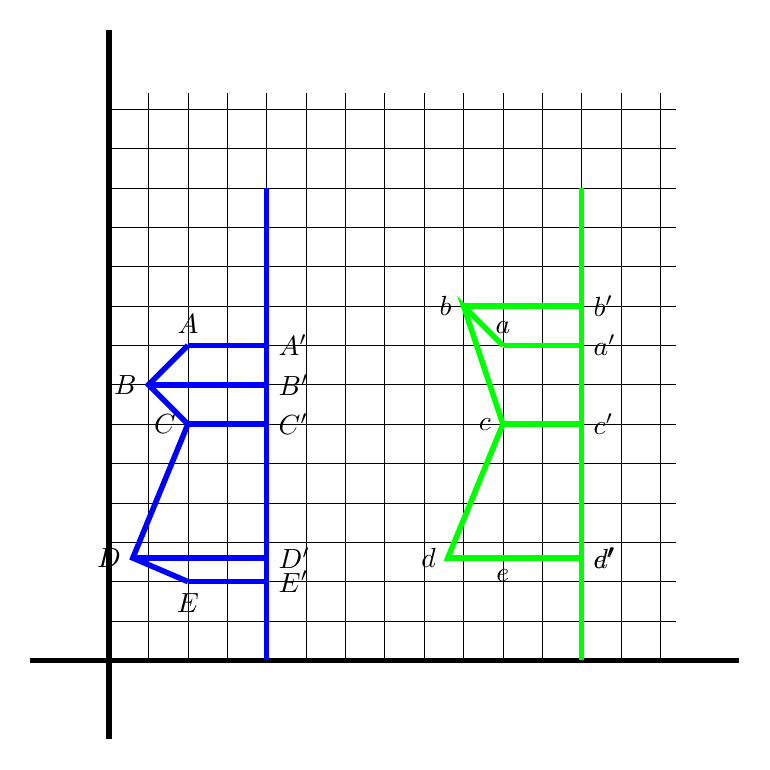
\begin{tikzpicture}[line width=2pt]
\draw (-1,0) -- (8,0);
\draw (0,-1) -- (0,8);
\draw[step=.5cm, very thin] (0,0) grid (7.2,7.2);

\coordinate [label=above:$A$] (A) at (1, 4);
\coordinate [label=left:$B$] (B) at (0.5, 3.5);
\coordinate [label=left:$C$] (C) at (1, 3);
\coordinate [label=left:$D$] (D) at (0.3, 1.3);
\coordinate [label=below:$E$] (E) at (1, 1);

\draw[blue] (A) -- (B) -- (C)  -- (D) -- (E);
\draw[blue] (2, 0) -- (2, 6);

\coordinate [label=right:$A'$] (A') at (2, 4);
\coordinate [label=right:$B'$] (B') at (2, 3.5);
\coordinate [label=right:$C'$] (C') at (2, 3);
\coordinate [label=right:$D'$] (D') at (2, 1.3);
\coordinate [label=right:$E'$] (E') at (2, 1);

\draw[blue] (A) -- (A');
\draw[blue] (B) -- (B');
\draw[blue] (C) -- (C');
\draw[blue] (D) -- (D');
\draw[blue] (E) -- (E');

\coordinate [label=above:$a$] (a) at (5, 4);
\coordinate [label=left:$b$] (b) at (4.5, 4.5);
\coordinate [label=left:$c$] (c) at (5, 3);
\coordinate [label=left:$d$] (d) at (4.3, 1.3);
\coordinate [label=below:$e$] (e) at (5, 1.3);

\draw[green] (a) -- (b) -- (c)  -- (d) -- (e);
\draw[green] (6, 0) -- (6, 6);

\coordinate [label=right:$a'$] (a') at (6, 4);
\coordinate [label=right:$b'$] (b') at (6, 4.5);
\coordinate [label=right:$c'$] (c') at (6, 3);
\coordinate [label=right:$d'$] (d') at (6, 1.3);
\coordinate [label=right:$e'$] (e') at (6, 1.3);

\draw[green] (a) -- (a');
\draw[green] (b) -- (b');
\draw[green] (c) -- (c');
\draw[green] (d) -- (d');
\draw[green] (e) -- (e');
\end{tikzpicture}
\caption{Monotonic polygonal chains}
\label{fig:monotonic_chain}
\end{figure}

\section{表格测试}
\begin{table}[htbp]
  \centering
  \begin{tabular}[htbp]{r|l}
    \toprule
    日期 & 任务 \\
    \midrule
    2011.5 & 完善此份文档 \\
    2011.6 & 完善安装脚本 \\
    \bottomrule
  \end{tabular}
  \caption{表格}
  \label{tab:table1}
\end{table}

\section{源代码高亮测试}

以下是\href{http://acm.zju.edu.cn/onlinejudge/showProblem.do?problemCode=1372}{ZOJ 1372}的解题c++代码:

\begin{lstlisting}[language=c++]
#include <iostream>
#include <string>
using namespace std;
 
const long max_points = 100;
const long infinity = 1000001;
 
int p, r, length, g[max_points][max_points];
bool flag;
 
class vertex
{
public:
    int distance;
    bool visited;
};
 
vertex v[max_points];
 
void initial()
{
    for(int i = 1; i <= p; i++)
        for(int j = 1; j <= p; j++)
            g[i][j] = infinity;
}
 
void prim(int origin)
{
    int temp_min;
    int temp_v = 0;
    int sum = 0;
 
    for(int i = 1; i <= p; i++)
    {
        v[i].distance = g[i][origin];
        v[i].visited = false;
    }
 
    v[origin].distance = 0;
    v[origin].visited = true;
 
    sum++;
 
    while (sum < p)
    {
        temp_min = infinity;
        for(int i = 1; i <= p; i++)
            if(v[i].visited == false && v[i].distance < temp_min)
            {
                temp_min = v[i].distance;
                temp_v = i;
            }
         
        if(temp_min < infinity)
        {
            length += v[temp_v].distance;
            v[temp_v].visited = true;
            sum++;
        }
        else
        {
            flag = true;
            break;
        }
 
        for(int i = 1; i <= p; i++)
        {
            if(v[i].visited == false && v[i].distance > g[i][temp_v])
            {
                v[i].distance = g[i][temp_v];
            }
        }
    }
}
 
int main(int argc, char *argv[])
{
    int a, b, c;
 
    while(cin >> p)
    {
        if(p == 0)
            break;
        cin >> r;
 
        initial();
 
        for(int i = 0; i < r; i++)
        {
            cin >> a >> b >> c;
            if(c < g[a][b])
                g[a][b] = g[b][a] = c;
        }
        length = 0;
        prim(1);
 
        cout << length << endl;
    }
 
    return 0;
} 
\end{lstlisting}

\section{数学公式测试}

著名的爱因斯坦质能方程(\ref{eq:emc2}):

\begin{equation}
  \label{eq:emc2}
  E=mc^2
\end{equation}

计算$f(x)=x^2$的不定积分(\ref{eq:2}):

\begin{equation}
  \label{eq:2}
  \int x^2 dx = \frac{1}{3} x^3
\end{equation}
\section{参考文件测试}
参考文件最好使用bibtex,关于bibtex的使用方法,你可以自行查阅相关文献。

这里是参考文献\cite{c_minigui}

%%%%%%%%%------------------------------------------------------------------------
%%%% 附录

% \appendix    
% \appendixpage
%% 将附录条目添加到contents
% \addappheadtotoc

%%%% 附录结束
%%%%%%%%------------------------------------------------------------------------

%
%%% 加入参考文献支持
%\bibliography{data/main}
%%% 解决目录中没有相应的参考文献的条目问题
%\addcontentsline{toc}{section}{\refname} 
%\end{document}
%%%% 正文部分结束
%%%%%%%%------------------------------------------------------------------------

%\restoregeometry
%\newpage

\tableofcontents

\thispagestyle{empty}
\addcontentsline{toc}{section}{授课计划}
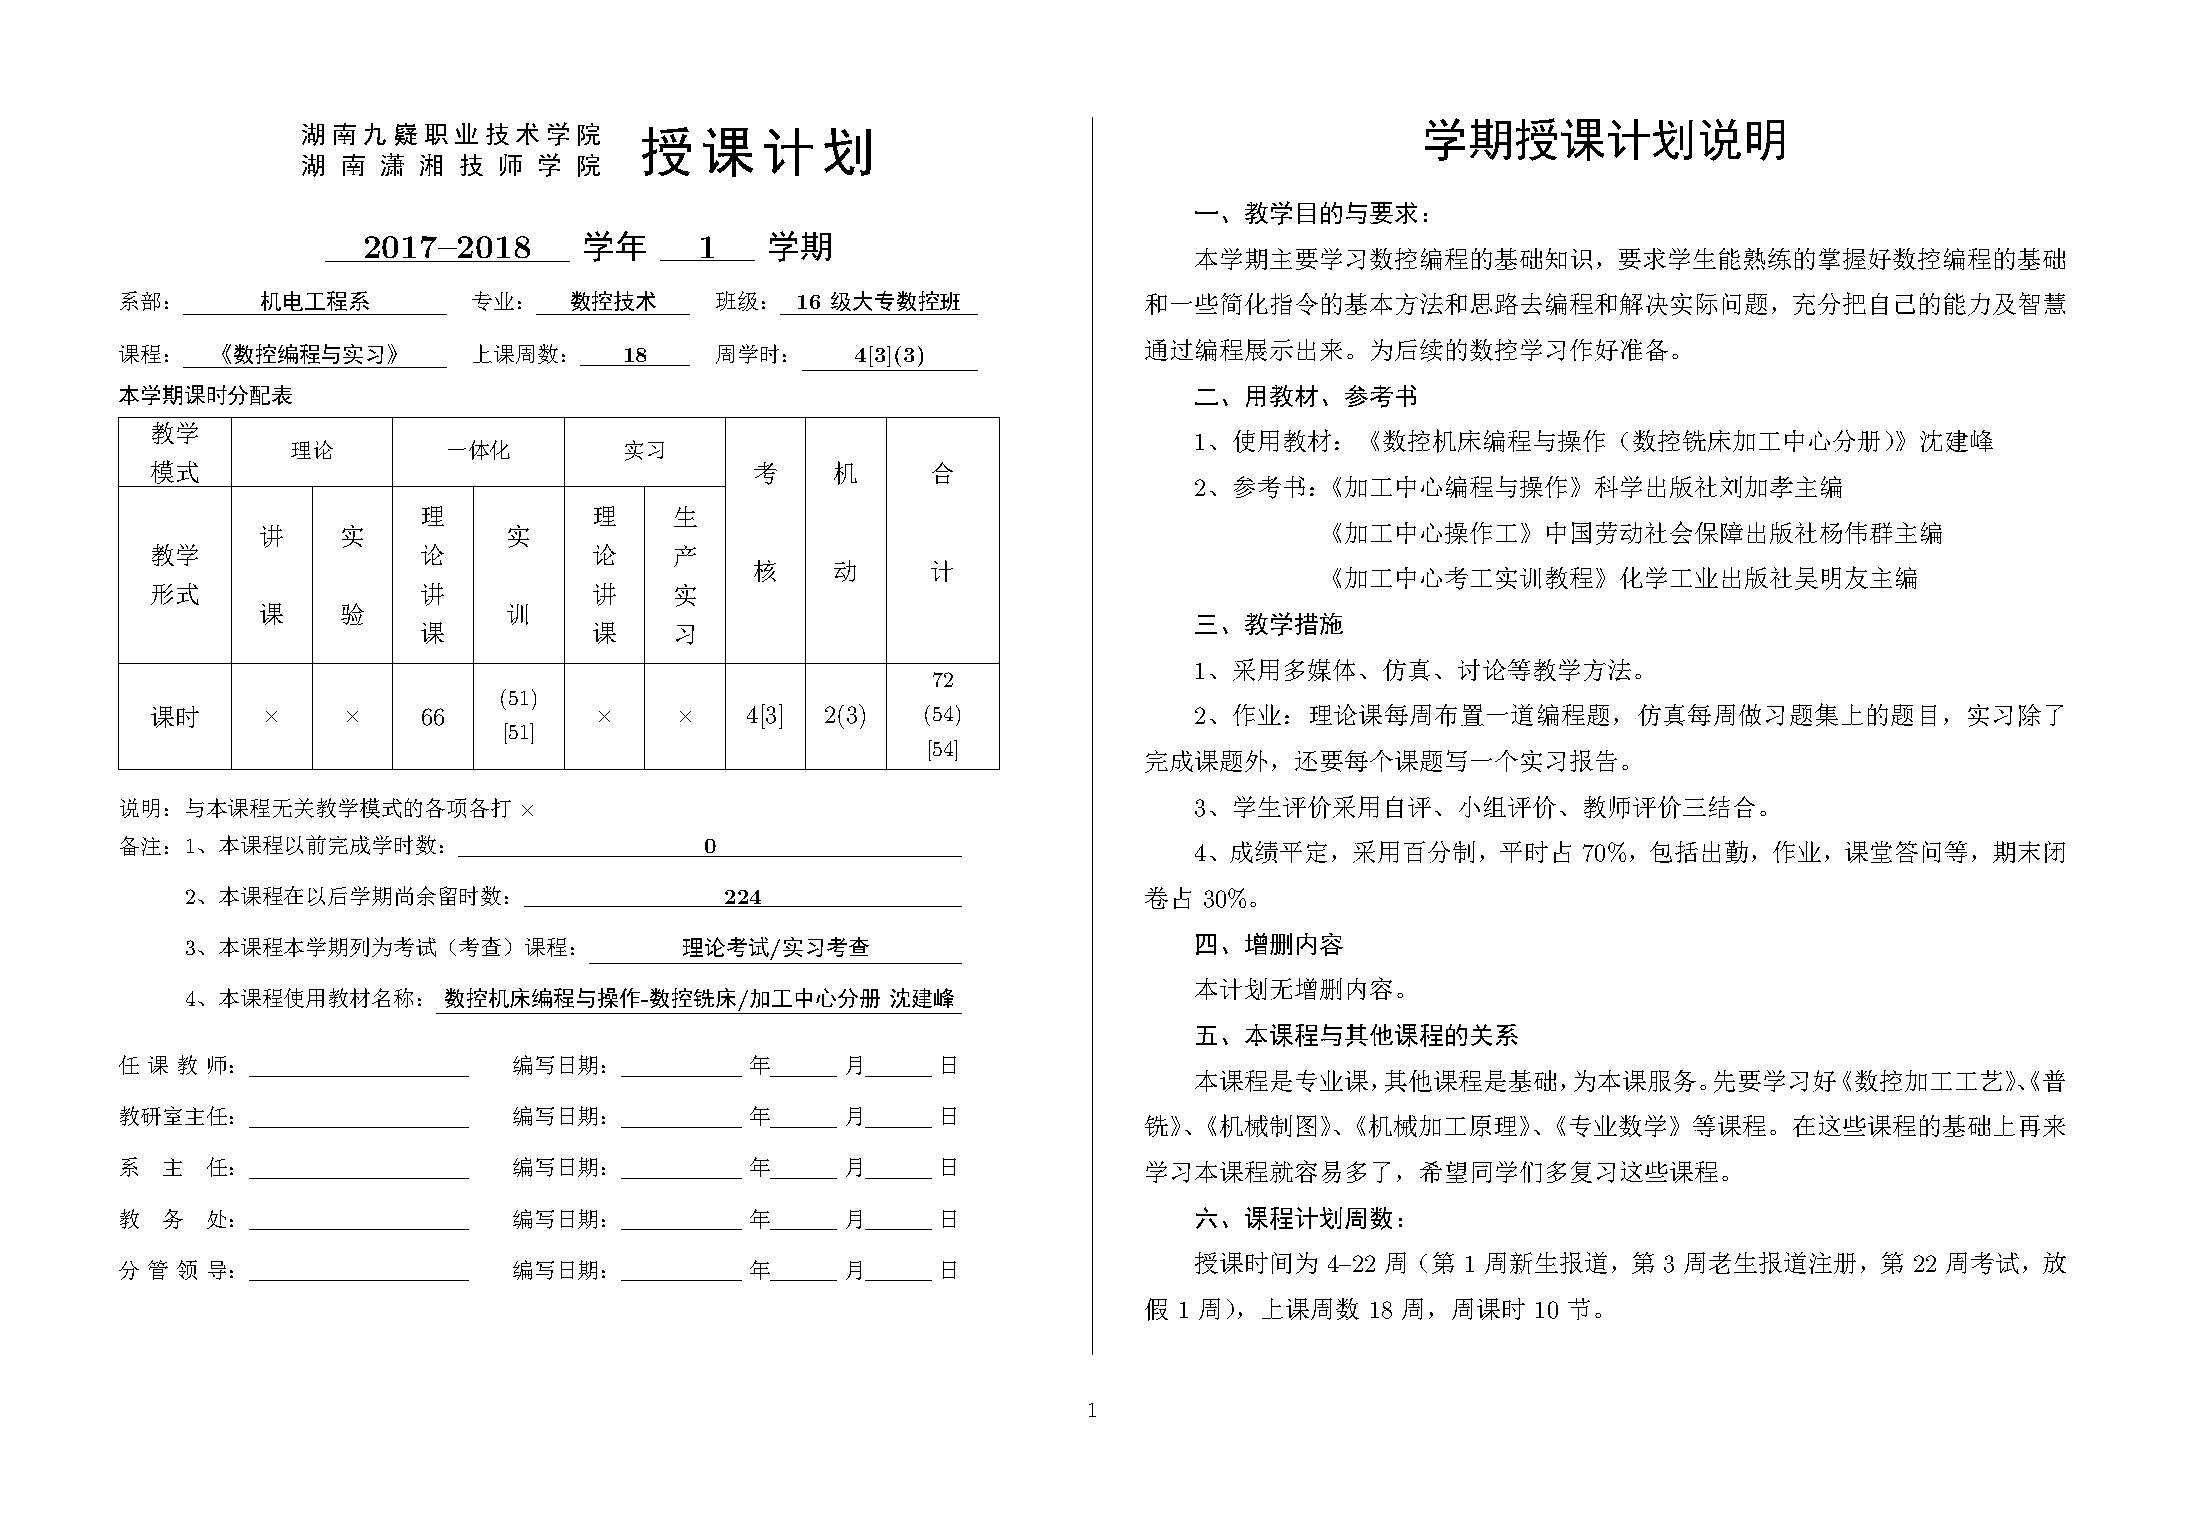
\includepdf[pages={-},landscape=true]{16jdzb-skjh.pdf}

\zihao{4}

\setcounter{page}{1}
\jxhj{%教学后记
	 }
\skrq{%授课日期
	2018年~~9月14日~~1-2节   }
\ktmq{%课题名称
	数控编程概术 }
\jxmb{%教学目标,每行前面要加 \item
	\item 了解数控技术的基本知识;
	\item 掌握数控机床的分类;
	\item 了解制造自动化技术的发展;}
\jxzd{%教学重点,每行前面要加 \item
	\item 了解数控技术的基本知识;
	\item 数控机床的分类;}
\jxnd{%教学难点,每行前面要加 \item
	\item 数控技术的基本知识;}
\jjff{%教学方法
	通过讲述、举例、演示法来说明;}

\makeshouye %制作教案首页

%%%%教学内容
\subsection{组织教学}
\begin{enumerate}[\hspace{2em}1、]
	\setlength{\itemsep}{0pt}
	\item 集中学生注意力;
	\item 清查学生人数;
	\item 维持课堂纪律;
\end{enumerate}
\subsection{复习导入及主要内容}
\begin{enumerate}[\hspace{2em}1、]
\item 自我介绍
\item 企业需要什么样的数控人才:\\
A:人品好:有道德、有理想、乐于助人。\\
B:精神面貌好:胆大心细,勇于思考、
能吃苦,不怕累、不怕脏。\\
C:能干事,有水平、速度快。\\
D:积极上进,乐于创新
\item 学习目标及要求:\\
A:会操作数控机床。快,准、细心。\\
B:能进行简单零件的工艺处理。会、经验积累。 \\
C:能进行简单零件的编程。思路清晰、编程细心、改错准快。\\
\end{enumerate}
跟着老师、多练习(作业)、准备充分、多想多问多看。
\subsection{教学内容及过程}
\subsubsection{制造自动化技术的发展} \marginpar{说明介绍}
1、人工控制——手动操作

2、刚性自动化——在20世纪40~50年代已相当成熟。应用传统的机械设计与制造工艺方法,采用专用机床和组合机床、自动单机或自动化生产线进行大批量生产。其特征是高生产率和刚性结构,很难实现生产产品的改变。引入的新技术包括继电器程序控制、组合机床等。

3、数控加工——包括数控(NC)和计算机数控(CNC)。特点是柔性好、加工质量高,适应于多品种、中小批量(包括单件产品)的生产。引入的新技术包括数控技术、计算机编程技术等。

4、柔性制造——其特征强调制造过程的柔性和高效率,适应于多品种、中小批量的生产。涉及的技术包括成组技术(GT)、计算机直接数控和分布式数控(DNC)、柔性制造单元(FMC)、柔性制造系统(FMS)、柔性加工线(FML)、离散系统理论和方法、仿真技术、车间计划与控制、制造过程监控技术、计算机控制与通信网络等。

5、计算机集成制造系统(CIMS)——其特征是强调全过程的系统性和集成性,以解决现代企业生存与竞争的 TQCS (Time-提供产品的时间,Quality-产品的质量,Cost-产品的成本,Service-产品的服务)问题。CIMS涉及的学科非常广泛,包括现代制造技术、管理技术、计算机技术、信息技术、自动化技术和系统工程等。

6、新的制造自动化模式——如智能制造、敏捷制造、虚拟制造、网络制造、全球制造、绿色制造等。

\subsubsection{数控技术的基本概念} \marginpar{互动提问}
1、数控技术

数控(Numerical Control)技术是用数字化的信息对某一对象进行控制的技术。
控制对象可以是位移、角度、速度等机械量,也可以是温度、压力流量、颜色等物理量,这些量的大小不仅是可以测量的,而且可以经A/D或D/A转换,用数字信号来表示。数控技术是近代发展起来的一种自动控制技术,是机械加工现代化的重要基础与关键技术。

2、数控加工

数控加工是指采用数字信息对零件加工过程进行定义,并控制机床进行自动运行的一种自动化加工方法。

数控加工是20世纪40年代后期为适应加工复杂外形零件而发展起来的一种自动化技术。1947年,美国帕森斯(Parsons)公司为了精确地制作直升机机翼、浆叶和飞机框架,提出了用数字信息来控制机床自动加工外复杂零件的设想。1949年美国空军为了能在短时间内制造出经常变更设计的火箭零件,与帕森斯公司和麻省理工学院(MIT)伺服机构研究所合作,于1952年研制成功世界上第一台数控机床——三坐标立式铣床,可控制铣刀进行连续空间曲面的加工,揭开了,数控加工技术的序幕。

3、数控机床

数控机床就是采用了数控技术的机床。
数控机床将零件加工过程所需的各种操作和步骤以及刀具与工件之间的相对位移量都用数字化的代码来表示,由编程人员编制成规定的加工程序,通过输入介质(磁盘等)送入计算机控制系统,由计算机对输入的信息进行处理与运算,发出各种指令来控制机床的运动,使机床自动地加工出所需要的零件。

特点有:高精度、高柔性、高效率、减轻工人的劳动强度,改善了劳动条件,有良好的经济效益,有利于生产的管理和现代化。

4、数控编程

数控编程(NC Programming)就是生成用数控机床进行零件加工数控程序的过程。
数控程序  是由一系列程序段组成,把零件的加工过程、切削用量、位移数据以及各种辅助操作,按机床的操作和运动顺序,用机床规定的指令及程序格式排列而成的一个有序指令集。如 N10 G00 X200.0 Y-39.0 M03 。

\subsubsection{数控机床的组成与工作过程}
1、数控机床的组成

A、输入输出设备

实现编制程序、输入程序、输入数据以及显示、存储和打印等功能。(如键盘、CRT显示器等)

B、数控系统

是数控机床的“大脑”和“核心”,通常由一台通用或专用计算机构成。它的功能是接受输入装置输入的加工信息,经过数控系统中的系统软件或逻辑电路进行译码、运算和逻辑处理后,发出相应的各种信号和指令给伺服系统,通过伺服系统控制机床的各个运用部件按规定要求动作。

C、伺服系统

伺服系统接收来自数控系统的指令信息,严格按指令信息的要求驱动机床的运动部件动作,以加工出符合要求的零件。伺服系统的伺服精度和动态响应是影响数控机床的加工精度、表面质量和生产率的重要因素之一。

D、机床本体

机床本体是数控机床的主体,包括:床身、立柱等去支承部件;主轴等运动部件;工件台、刀架以及运动执行部件、传动部件;此外还有冷却、润滑、转位和夹紧等辅助装置。

2、数控机床的工作过程

A、准备阶段

根据加工零件的图纸,确定有关加工数据(刀具轨迹坐标点、加工的切削用量、刀具尺寸信息等)根据工艺方案、夹具选用、刀具类型选择等确定有关期货辅助信息。

B、编程阶段

C、准备信息载体

D、加工阶段

加工




\subsubsection{数控机床的种类}
1、按工艺用途分类

A、金属切削类数控机床    数控车床、数控铣床、数控磨床、数控镗床以及加工中心。

B、金属成型类数控机床    数控折弯机、数控组合冲床、数控弯管机、数控回转头压力机等。这类机床起步晚,但目前发展很快。

C、数控特种加工机床    数控线切割机床、数控电火花机床、数控火焰切割机床、数控激光切割机床等。

D、其它类型数机床    数控三坐标测量机等。

2、按运动方式分类

A、点位控制数控机床    刀具点到点

B、直线控制数控机床    刀具平行于某一坐标轴移动

C、轮廓控制数控机床    刀具沿两个或两个以上的坐标轴同时移动。

3、按控制方式分类

A、开环控制系统

B、半闭环控制系统

C、闭环数控系统

4、按数控系统功能水平分类

数控机床按数控系统的功能水平可分为低、中、高三档。不同时期其划分标准也不同:

分辨率和进给速度

伺服进给类型

联运轴数

通信能力

显示功能

内装PLC

主CPU

高速、高效、高精度、高可靠性

模块化、智能化、柔性化和集成化



\subsubsection{数控机床的坐标系}
\subsection{课堂小结}
\begin{enumerate}[1、]
\item 制造自动化的发展;
\item 数控技术的基本概念;
\item 数控机床的组成与工作过程;
\item 数控机床的种类;
\item 数控机床的坐标系。
\end{enumerate}
\subsection{布置作业}
\begin{enumerate}[1、]
\item 简述数控机床的组成部分?
\item 简述数控机床的分类?
\item 数控机床有哪些特点?
\end{enumerate}
\vfill

\jxhj{%教学后记
	}
\skrq{%授课日期
	2018年~~ 9月14日~~3-4节}
\ktmq{%课题名称
	程序的基本结构 }
\jxmb{%教学目标,每行前面要加 \item
	\item 掌握数控程序的组成与结构。;

	\item 掌握数控编程的方法;

	\item 掌握编写数控程序的基本思路;

	\item 了解数控常见指令;}
\jxzd{%教学重点,每行前面要加 \item
	\item 数控程序的组成与结构;

	\item 编写数控程序的基本思路;}
\jxnd{%教学难点,每行前面要加 \item
	\item 数控程序的组成与结构;}
\jjff{%教学方法
	通过讲述、举例、演示法来说明;}

\makeshouye %制作教案首页

%%%%教学内容
\subsection{组织教学}
\begin{enumerate}[1、]
	\item 集中学生注意力;
	\item 清查学生人数;
	\item 维持课堂纪律;
\end{enumerate}
\subsection{复习导入及主要内容}
\begin{enumerate}[1、]
	\item 制造自动化的发展;
	\item 数控技术的基本概念;
	\item 数控机床的组成与工作过程;
	\item 数控机床的种类;
	\item 数控机床的坐标系。
\end{enumerate}
\subsection{教学内容及过程}
\subsubsection{数控编程的坐标系及假设}
\begin{enumerate}[1、]
	\item 数控机床的标准坐标系;
	\subitem A、右手笛卡尔直角坐标系;
	\subitem B、数控机床坐标系的判定方法;
	\subitem C、工件静止刀具移动的假设。 
	\item 机床坐标系/机械坐标系;
	\item 工件坐标系;
	\item 零点偏移;
	\item 局部坐标系;
	\item 极坐标系;
\end{enumerate}
\subsubsection{数控程序的结构}
\begin{enumerate}[1、]
	\item 程序展示;
	\item 程序结构;
	\item 程序;
	\item 程序段;
	\item 地址;
	\item 程序段结束符。
\end{enumerate}
\subsubsection{数控程序的指令}
\begin{enumerate}[1、]
	\item 准备功能;
	\item 辅助功能;
	\item 其他;
	\item 模态指令/非模态指令;
	\item 指令分组。
\end{enumerate}
\subsubsection{数控编程的方式}
\begin{enumerate}[1、]
\item 手工编程
利用一般的计算工具,通过各种数学方法,人工进行刀具轨迹的运算,并进行指令编制。该方式比较简单,容易掌握。适用于中等复杂程度、计算量不大的零件编程,对机床操作人员来讲必须掌握的。

手工编程的步骤:

A、图样分析  包括对零件轮廓形状、有关标注(尺寸公差、形状和位置公差及表面质量要求等)及材料和热处理等项要求进行分析。

B、辅助准备  包括确定机床和夹具、机床坐标系、编程坐标系、对刀方法、对刀点位置及机械间隙值等。

C、工艺处理  其内容包括加工余量与分配、刀具的运动方向与加工路线、切削用量及确定程序编制的允许误差等方面。

D、数学处理  包括尺寸分析与作图、选择处理方法、数值计算及对拟合误差的分析和计算等。

E、填写加工程序单  按照数控系统规定的程序格式和要求,填写零件的加工程序单及加工条件等内容。

F、制备控制介质  数控机床在自动输入加工程序时,必须输入用的控制介质。如穿孔带、磁带或软盘等。

H、程序校验  包括对程序单的填写、控制介质的制备、刀具运动轨迹及等项内容所进行的单项或综合校验工作。

手工编程在目前仍是广泛采用的编程方式,即使在自动编程高速发展的将来,手工编程的重要地位也不可取代。

\item 自动编程  

利用计算机(含外围设备)和相应的前置、后置处理程序对程序对零件源程序进行处理,以得到加工程序单各数控带的一种编程方式。

对于曲线轮廓、三维曲面等复杂型面。一般采用自动编程。

在工作站或个人PC上利用CAD/CAM系统进行零件的设计、分析及加工编程。它适用于各类柔性制造系统(FMS)和计算机集成制造系统(CIMS)。

\end{enumerate}
\subsubsection{编写程序的基本思路}
程序初始化(安全保护)--------辅助准备(换刀,主轴启动,切削液开)--------定位到起刀点--------快速下刀--------工进下刀--------走加工轮廓--------提刀---------快速提刀到安全平面-------程序结束(换刀,主轴停止,切削液关,程序返回等)
\subsection{课堂小结}
\begin{enumerate}[1、]
\item 数控编程的坐标系及假设;

\item 数控程序的结构;
\item 数控程序的指令;
\item 数控编程的方式;
\item 编写程序的基本思路。
\end{enumerate}
\vfill
\subsection{布置作业}
\begin{enumerate}[1、]
	\item 写出数控程序的基本结构。
	\item 数控编程的方式有哪些?
\end{enumerate}
\vfill
\jxhj{%教学后记
	}
\skrq{%授课日期
	2017年9月12日 4-5节}
\ktmq{%课题名称
	基本指令及写程序思路 }
\jxmb{%教学目标,每行前面要加 \item
	\item 掌握手工编程的流程;
    \item 掌握基本指令;
    \item 编写矩形凸台的程序;
    \item 掌握编程基本思路。}
\jxzd{%教学重点,每行前面要加 \item
	\item 掌握G90、G91、G0、G1指令;
	\item 编写数控程序的基本思路;}
\jxnd{%教学难点,每行前面要加 \item
	\item 掌握G90、G91、G0、G1指令;}
\jjff{%教学方法
	通过讲述、举例、演示法来说明;}

\makeshouye %制作教案首页

%%%%教学内容
\subsection{组织教学}
\begin{enumerate}[1、]
	\item 集中学生注意力;
	\item 清查学生人数;
	\item 维持课堂纪律;
\end{enumerate}
\subsection{复习导入及主要内容}
\begin{enumerate}[1、]
    \item 数控编程的坐标系及假设;
    \item 数控程序的结构;
    \item 数控程序的指令;
    \item 数控编程的方式;
    \item 编写程序的基本思路。
\end{enumerate}
\subsection{教学内容及过程}
\subsubsection{案例分析}

在数控铣床或加工中心上加工如图\ref{fig:3-1}所示的零件,试完成程序的编写,已知毛坯为 $\Phi$ 110*30。

\begin{figure}
    \centering
    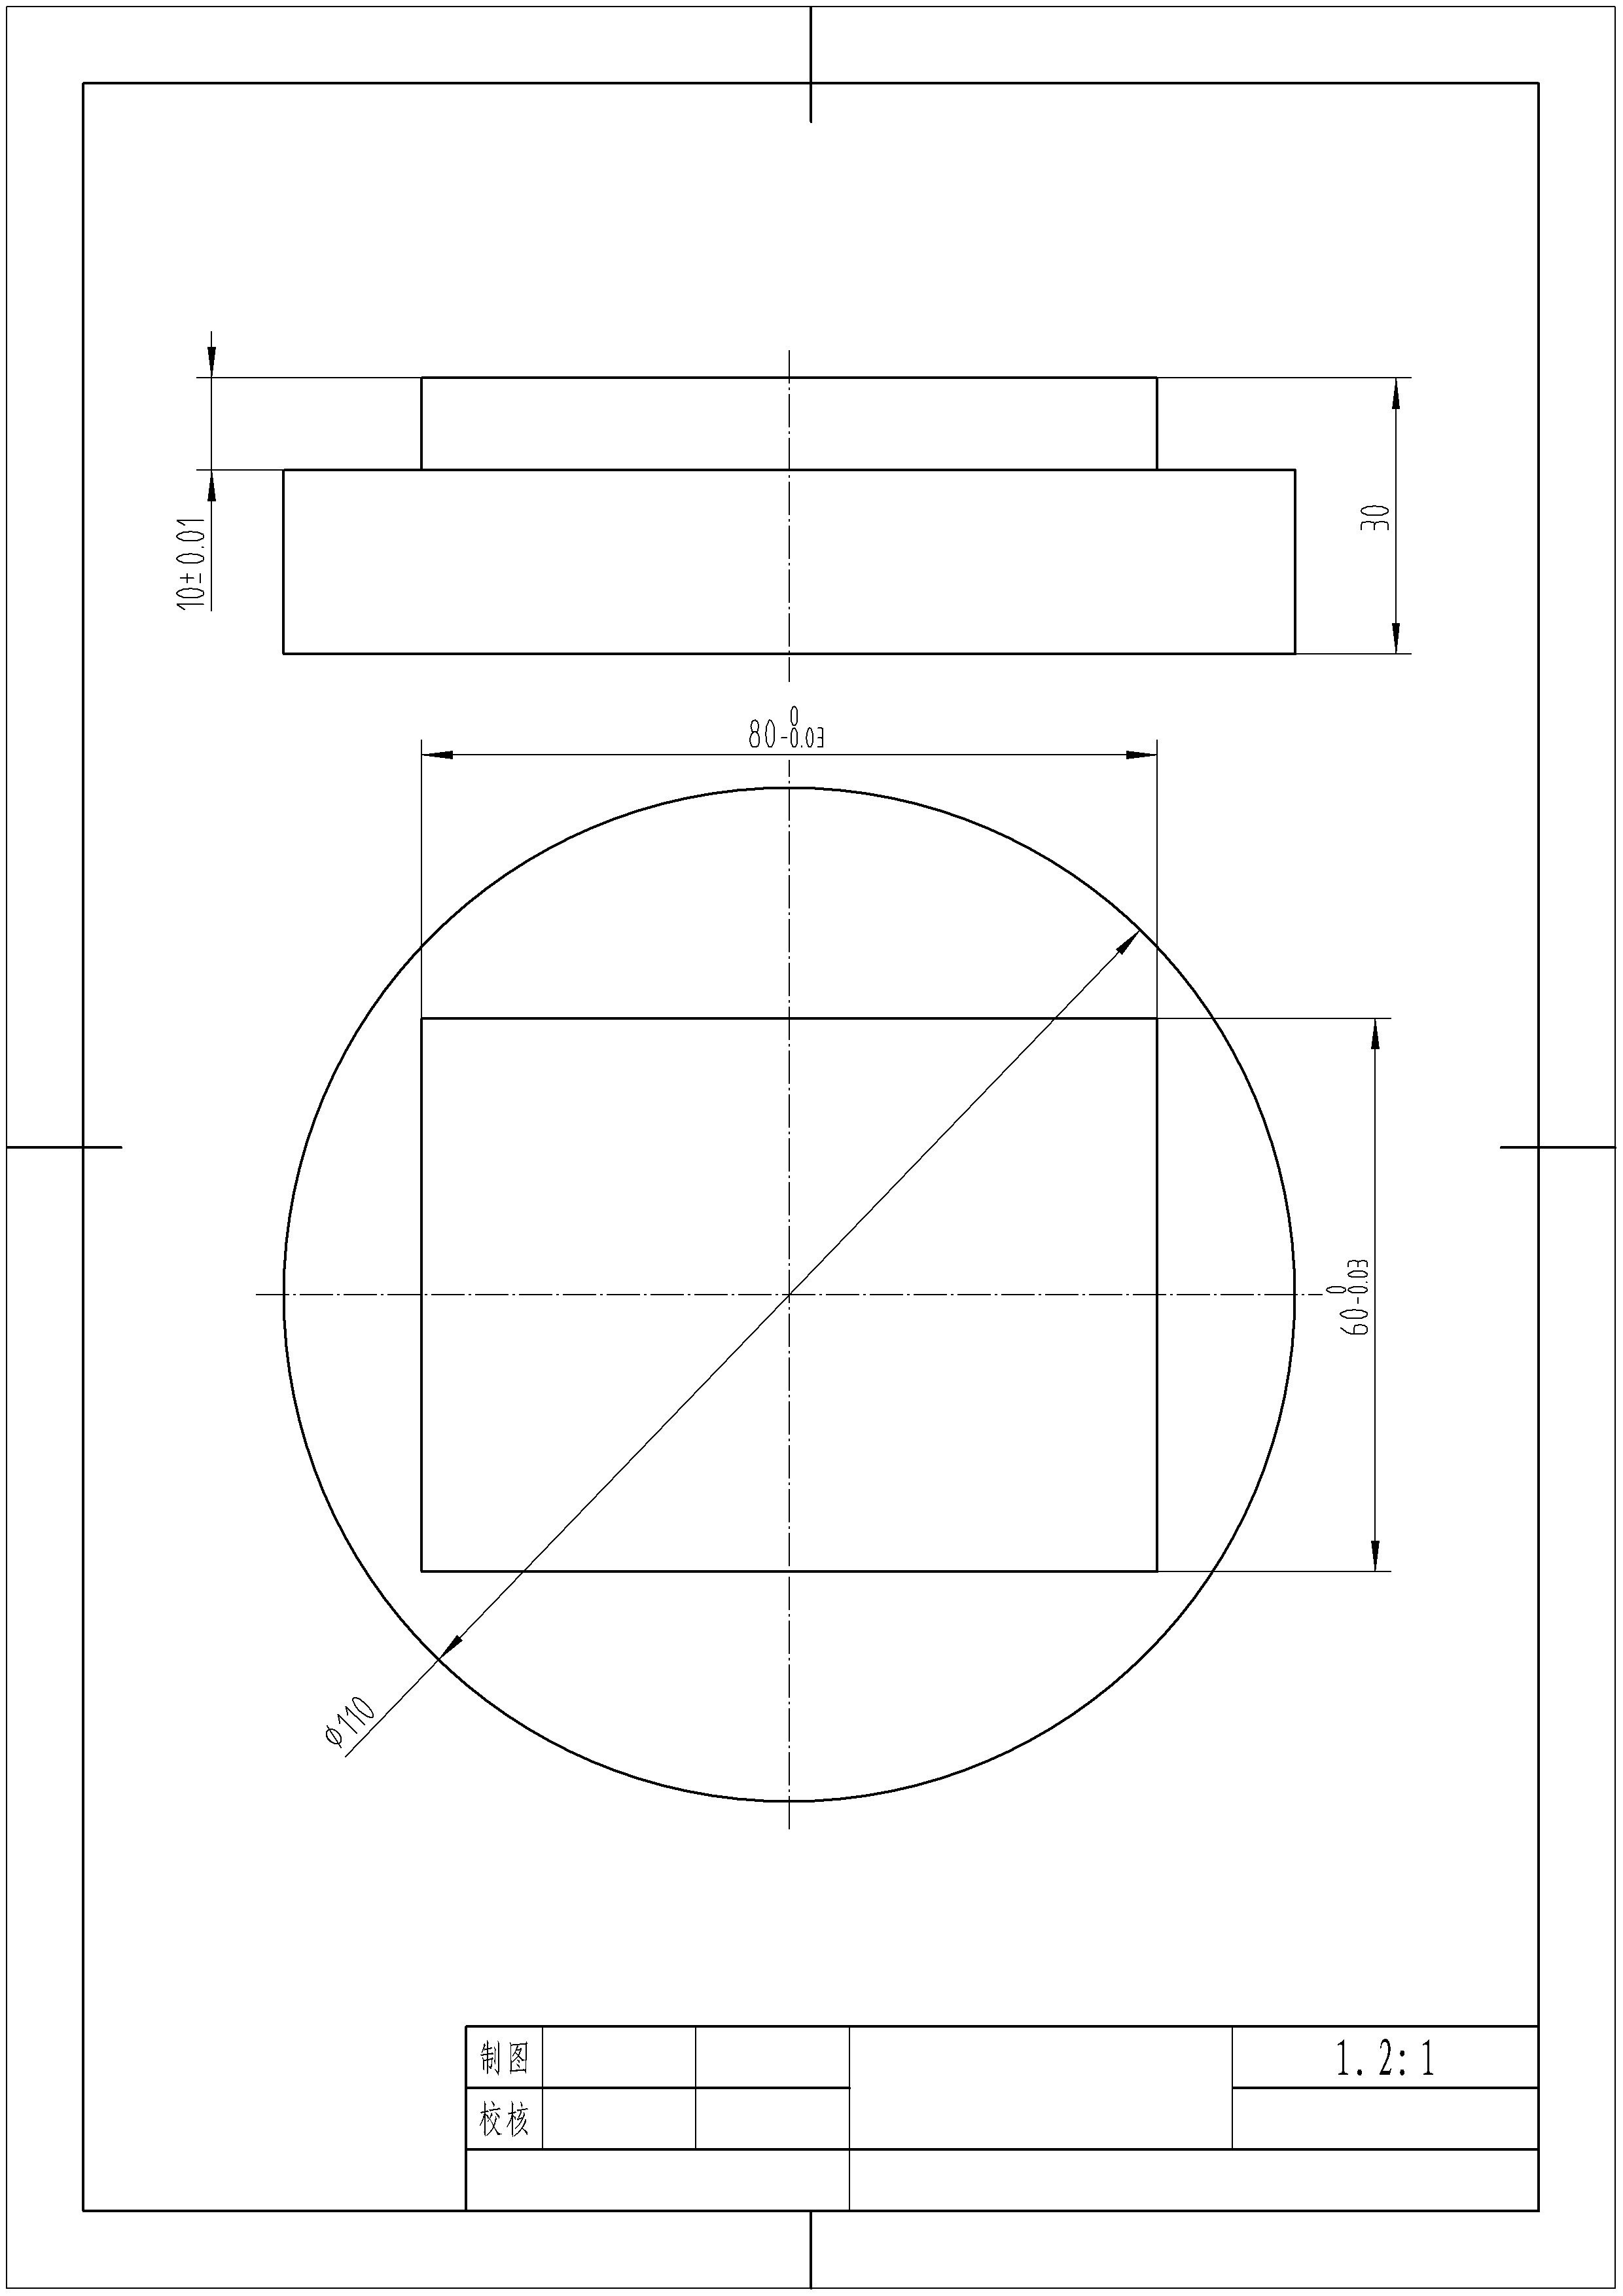
\includegraphics[width=0.8\linewidth,trim=50 150 50 100,clip]{data/image/3-1.jpg}
    \caption{}
    \label{fig:3-1}
\end{figure}

\begin{enumerate}[1、]
    \item 图样分析;
    \item 确定加工内容;
    \item 确定装夹及工件坐标系;
    \item 确定刀具及切削用量;
    \item 确定工序及走刀路线;
    \item 计算点坐标;
    \item 编写程序单。
\end{enumerate}

\subsubsection{程序名}
1、Fanuc的程序号与Siemens的程序名

Fanuc中用程序号区分各程序,程序号由位址O跟4位数字构成;是号,也就是说O0001号与O1号,表示同一个程序。

注意:1-7999为用户区域

8000-8999为加锁用户区域

9000-9999为厂方提供(扩展功能如O9001为换刀程序,也是加锁的)

所以用户最好别用8000-9999这些号码

2、Siemens中用程序名来区分各程序,确定程序名的规则是:

A、开始的两个符号必须是字母

B、其后的符号可以是字母,数字或下划线

C、最多为16个字符

D、不得使用分隔符

\subsubsection{安全注销指令}
1、G54-G59  选用工件坐标系,(后面讲)。

2、G17-G19  加工平面选择:

G17:XY平面 第一轴为X轴

G18:YZ平面 第一轴为Y轴

G19: ZX平面 第一轴为Z轴

圆弧指令、刀具半径补偿指令、钻孔指令等使用之前有设定平面。

3、G40、G49、G80 取消半径补偿、长度补偿、钻孔循环。

4、G90、G91 绝对坐标编程 增量坐标编程

G90指令按绝对坐标方式设定输入坐标,即移动指令终点的坐标值X、Y、Z都是以工件坐标系统坐标原点(程序零点)为基准来计算。

G91指令按增量坐标方式设定输入坐标,即移动指令终点的坐标值X、Y、Z都是以始点为基准来计算,再根据终点相对于始点的方向判断正负,与坐标轴正方向一致则取正,相反取负。

一般用G90,需要时采用G91,用完应立即改成G90。

\subsubsection{主轴正反转}
M3 S\verb|____| 主轴正转,其中S设定主轴转速,单位为r/min.

注意:本学校的机床,只有加工中心可以用S,数控铣床是机械调速,S无效,Siemens上不能使用S,不然机床会一直等主轴到达设定的转速后,才接着执行后面的程序。

\subsubsection{位移指令G0、G1}
定位(G0)

G00指令使刀具以绝对或相对指令快速移到工件系统指定的位置。在绝对指令状态下,编程端点的坐标值。在相对指令状态下编程中刀具移动的距离。

[ 格式 ]

G00 IP\_\_;

IP\_\_ :
对于绝对指令,端点的坐标值。对于相对指令,是指刀具移动的距离。

[ 说明 ]

刀具轨迹通常不是一条直线。

G00指令的快速移动速度是由参数No.1420由机床制造商来设定的。在实际执行G00时,刀具在单节的开始加速到预先指定的速度并在单节的结束减速。在确认到位后执行下一单节。到位的含义是指进给马达在指定的误差范围内。这个范围是由制造商在参数No.1826中设定的。

刀具沿直线移动。

[ 格式 ]

G01 IP\_\_ F\_\_ ;

IP\_\_ : 对于绝对指令,指端点的坐标,相对指令是指刀具移动的距离。

F\_\_ : 刀具进给的速度(进给率)

[ 说明 ]

刀具以指定的进给率F沿直线移动到指定的位置。

进给率F有效直到赋予新值,不需要在每个单节都指定。

F码指定的进给率是沿刀具轨迹测量的。

如果不指定F值,则认为进给率为零。

每个轴的进给率方向如下:

[ 限制 ]

G01 αα ββ γγ ζζ Ff  ;

α轴方向的进给率:Fα=α/L ×f

β轴方向的进给率:Fβ=β/L ×f

γ轴方向的进给率:Fγ=γ/L ×f

ζ轴方向的进给率:Fζ=ζ/L ×f

L2 = α2 + β2 + γ2 + ζ2

[ 举例 ]

■直线插补


\subsubsection{编写程序的基本思路}
程序初始化(安全保护)--------辅助准备(换刀,主轴启动,切削液开)--------定位到起刀点--------快速下刀--------工进下刀--------走加工轮廓--------提刀---------快速提刀到安全平面-------程序结束(换刀,主轴停止,切削液关,程序返回等)
\subsection{课堂小结}
\begin{enumerate}[1、]
\item 案例分析;
\item 指令讲解;
\item 编写程序;
\item 编写程序的基本思路。
\end{enumerate}
\vfill
\subsection{布置作业}
\begin{enumerate}[1、]
	\item 自定尺寸,编写加工一个矩形外形的程序?
\end{enumerate}
\vfill
\jxhj{%教学后记
	}
\skrq{%授课日期
	2017年9月14日 4-5节}
\ktmq{%课题名称
	基本指令(一) }
\jxmb{%教学目标,每行前面要加 \item
	\item 掌握G1与G0的区别。
    \item 掌握G2/G3的基本应用。
    \item 掌握编写数控程序的基本思路。
    \item 了解数控常见指令。}
\jxzd{%教学重点,每行前面要加 \item
	\item 掌握G1与G0的区别;
	\item 掌握G2/G3的基本应用;}
\jxnd{%教学难点,每行前面要加 \item
	\item 掌握G2/G3的基本应用;}
\jjff{%教学方法
	通过讲述、举例、演示法来说明;}

\makeshouye %制作教案首页

%%%%教学内容
\subsection{组织教学}
\begin{enumerate}[1、]
	\item 集中学生注意力;
	\item 清查学生人数;
	\item 维持课堂纪律;
\end{enumerate}
\subsection{复习导入及主要内容}
\begin{enumerate}[1、]
\item 案例分析;
\item 指令讲解;
\item 编写程序;
\item 编写程序的基本思路。
\end{enumerate}


\textbf{G0与G1的区别}

\begin{enumerate}[1、]
\item 指令格式不同:G1使用前必须用F设定进给速度,G0的速度与F无关 
\item 运动轨迹不同:G0为快速定位,其路径可能为直线,也可能为折线。G1为直线插补,其路径为直线。
\item 进给速度不同:G0的速度由机床参数及快速倍率决定,档位少。G1的速度由F及进给倍率决定,可调档位多。
\item 功能用途不同:G0用于加工前的定位及加工后的提刀,G1用于车削加工
\end{enumerate}
注意:

新学的同学用G1 F2000 代替 G0 (可控与不可控)

不要三坐标编程,定位时,先提刀,再定位。

\subsection{教学内容及过程}
\subsubsection{案例分析}

在数控铣床或加工中心上加工如图\ref{fig:4-1}所示的零件,试完成程序的编写,已知毛坯为 $\Phi$ 110*30。

\begin{figure}[h]
    \centering
    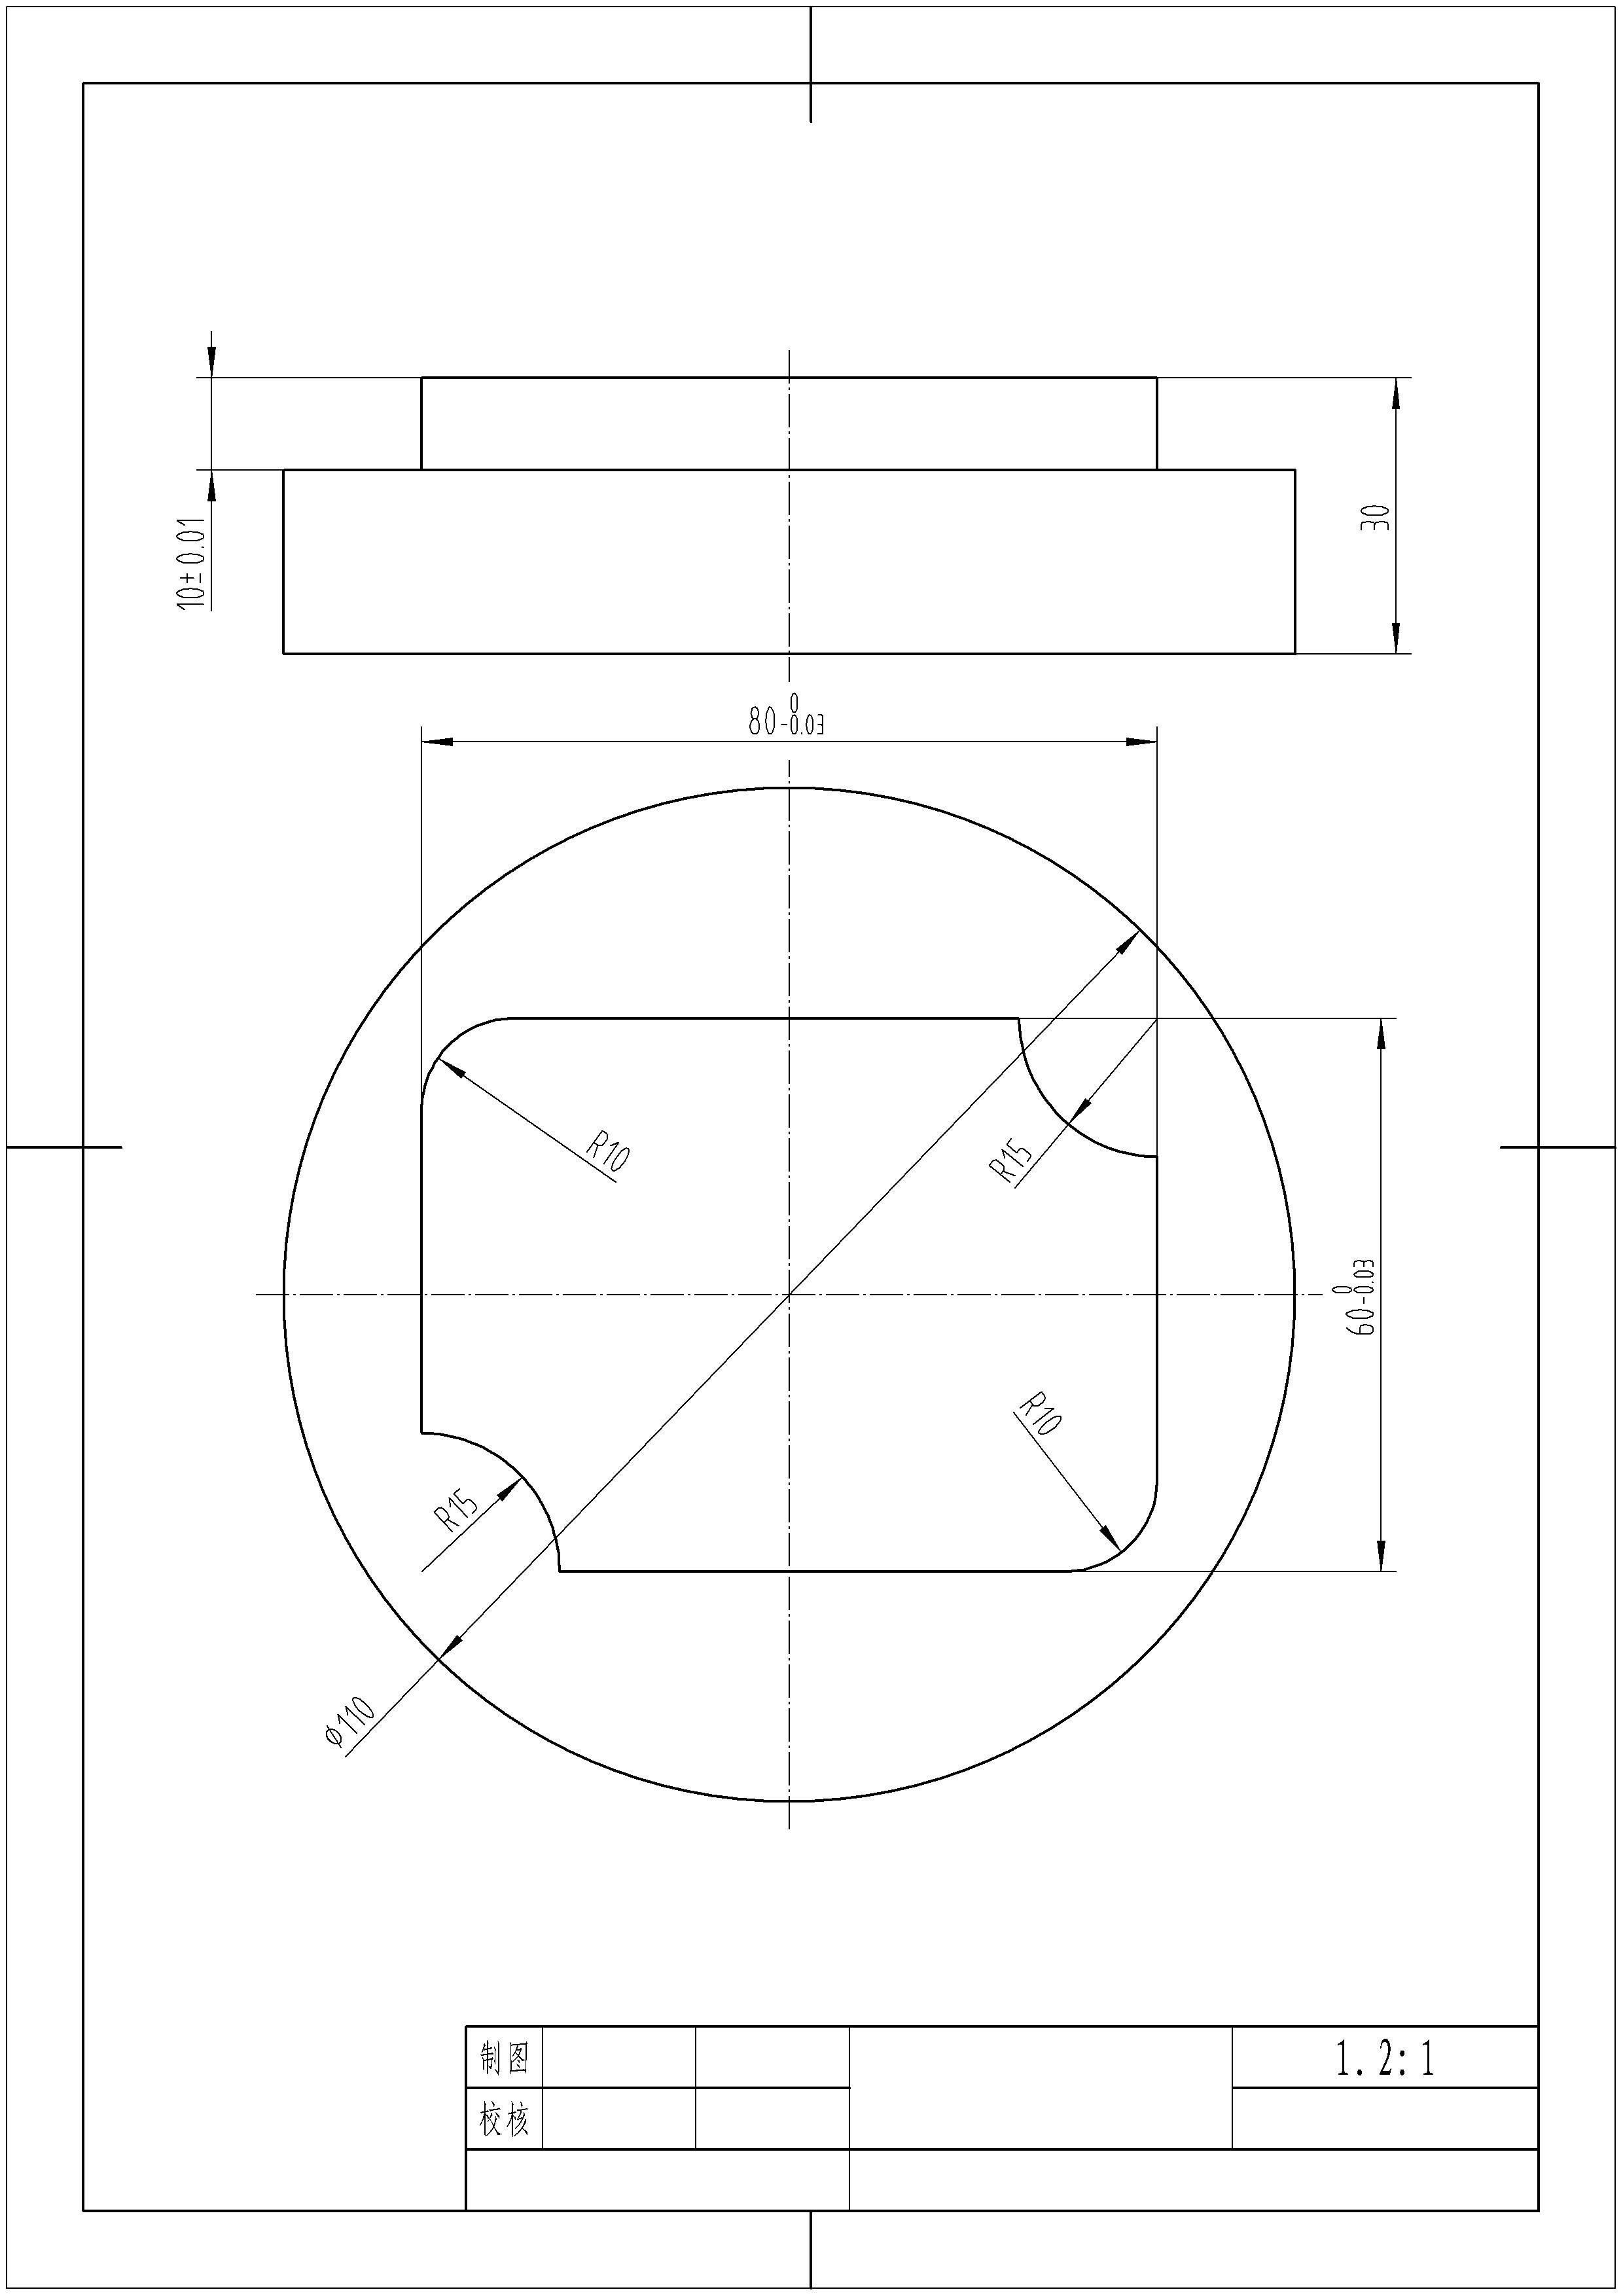
\includegraphics[width=0.8\linewidth,trim=50 150 50 100,clip]{data/image/4-1.jpg}
    \caption{}
    \label{fig:4-1}
\end{figure}

\begin{enumerate}[1、]
    \item 图样分析;
    \item 确定加工内容;
    \item 确定装夹及工件坐标系;
    \item 确定刀具及切削用量;
    \item 确定工序及走刀路线;
    \item 计算点坐标;
    \item 编写程序单。
\end{enumerate}

\subsubsection{G02/G03指令(只讲R编程)}

常见的圆弧标注—— 半径

起点——终点——半径

圆弧插补指令:

1、[格式]
XpYp平面的圆弧   
G17  G2/G3  X\_ Y\_ R\_ F\_
ZpXp平面的圆弧   
G18 G2/G3 Z X R F 
YpZp平面的圆弧   
G19 G2/G3 Y Z R F
对于我们学校的一般用G17平面

指令格式的说明

G17	指定圆弧在XpYp平面

G18	指定圆弧在XpZp平面

G19	指定圆弧在YpZp平面

G02	顺时针方向圆弧插补(CW)

G03	逆时针方向圆弧插补(CCW)

Xp\_\_	X轴或平行于X轴的指令值(由参数No.1022设定)

Yp\_\_	Y轴或平行于Y轴的指令值(由参数No.1022设定)

Zp\_\_	Z轴或平行于Z轴的指令值(由参数No.1022设定)

R\_\_	圆弧半径指定的带符号的圆弧半径

F\_\_	沿圆弧的进给率 



2、圆弧插补的方向

在XpYp平面(ZpXp平面或YpZp平面)“顺时针方向”(G02)和“逆时针方向”(G03)是从笛卡尔坐标系的Zp轴(Yp轴或Xp轴)去看正负方向来决定的,

3、目标点坐标

用位址Xp,Yp,Zp指定的圆弧的端点是根据G90还是G91来表达是绝对值还是相对值。

对于相对值, 终点的距离要从指定圆弧的起点来看。

4、举例:

A-B   G91   G90 

……   ( 学生练习)




\subsubsection{编写程序的基本思路}
程序初始化(安全保护)--------辅助准备(换刀,主轴启动,切削液开)--------定位到起刀点--------快速下刀--------工进下刀--------走加工轮廓--------提刀---------快速提刀到安全平面-------程序结束(换刀,主轴停止,切削液关,程序返回等)
\subsection{课堂小结}
\begin{enumerate}[1、]
\item 案例分析;
\item 指令讲解;
\item 编写程序;
\item 编写程序的基本思路。
\end{enumerate}
\vfill
\subsection{布置作业}
\begin{enumerate}[1、]
	\item 自定尺寸,编写加工一个矩形外形的程序?
\end{enumerate}
\vfill
\jxhj{%教学后记
	}
\skrq{%授课日期
	2017年9月21日 4-5节}
\ktmq{%课题名称
	基本指令(二) }
\jxmb{%教学目标,每行前面要加 \item
	\item 掌握G2/G3半径-R的使用;
    \item 掌握G2/G3圆心编程的使用;
    \item 能用G2/G3进行程序的编写;
    \item 掌握编写数控程序的基本思路。}
\jxzd{%教学重点,每行前面要加 \item
	\item G2/G3半径-R的使用;
	\item G2/G3圆心编程的使用;}
\jxnd{%教学难点,每行前面要加 \item
	\item G2/G3圆心编程的使用;}
\jjff{%教学方法
	通过讲述、举例、演示法来说明;}

\makeshouye %制作教案首页

%%%%教学内容
\subsection{组织教学}
\begin{enumerate}[1、]
	\item 集中学生注意力;
	\item 清查学生人数;
	\item 维持课堂纪律;
\end{enumerate}
\subsection{复习导入及主要内容}
\begin{enumerate}[1、]
\item 案例分析;
\item 指令讲解G2/G3;
\item 编写程序;
\item 编写程序的基本思路。
\end{enumerate}

\textbf{案例分析}

在数控铣床或加工中心上加工如图\ref{fig:5-1}所示的零件,试完成程序的编写,已知毛坯为 $\Phi$ 110*30。

\begin{figure}[h]
    \centering
    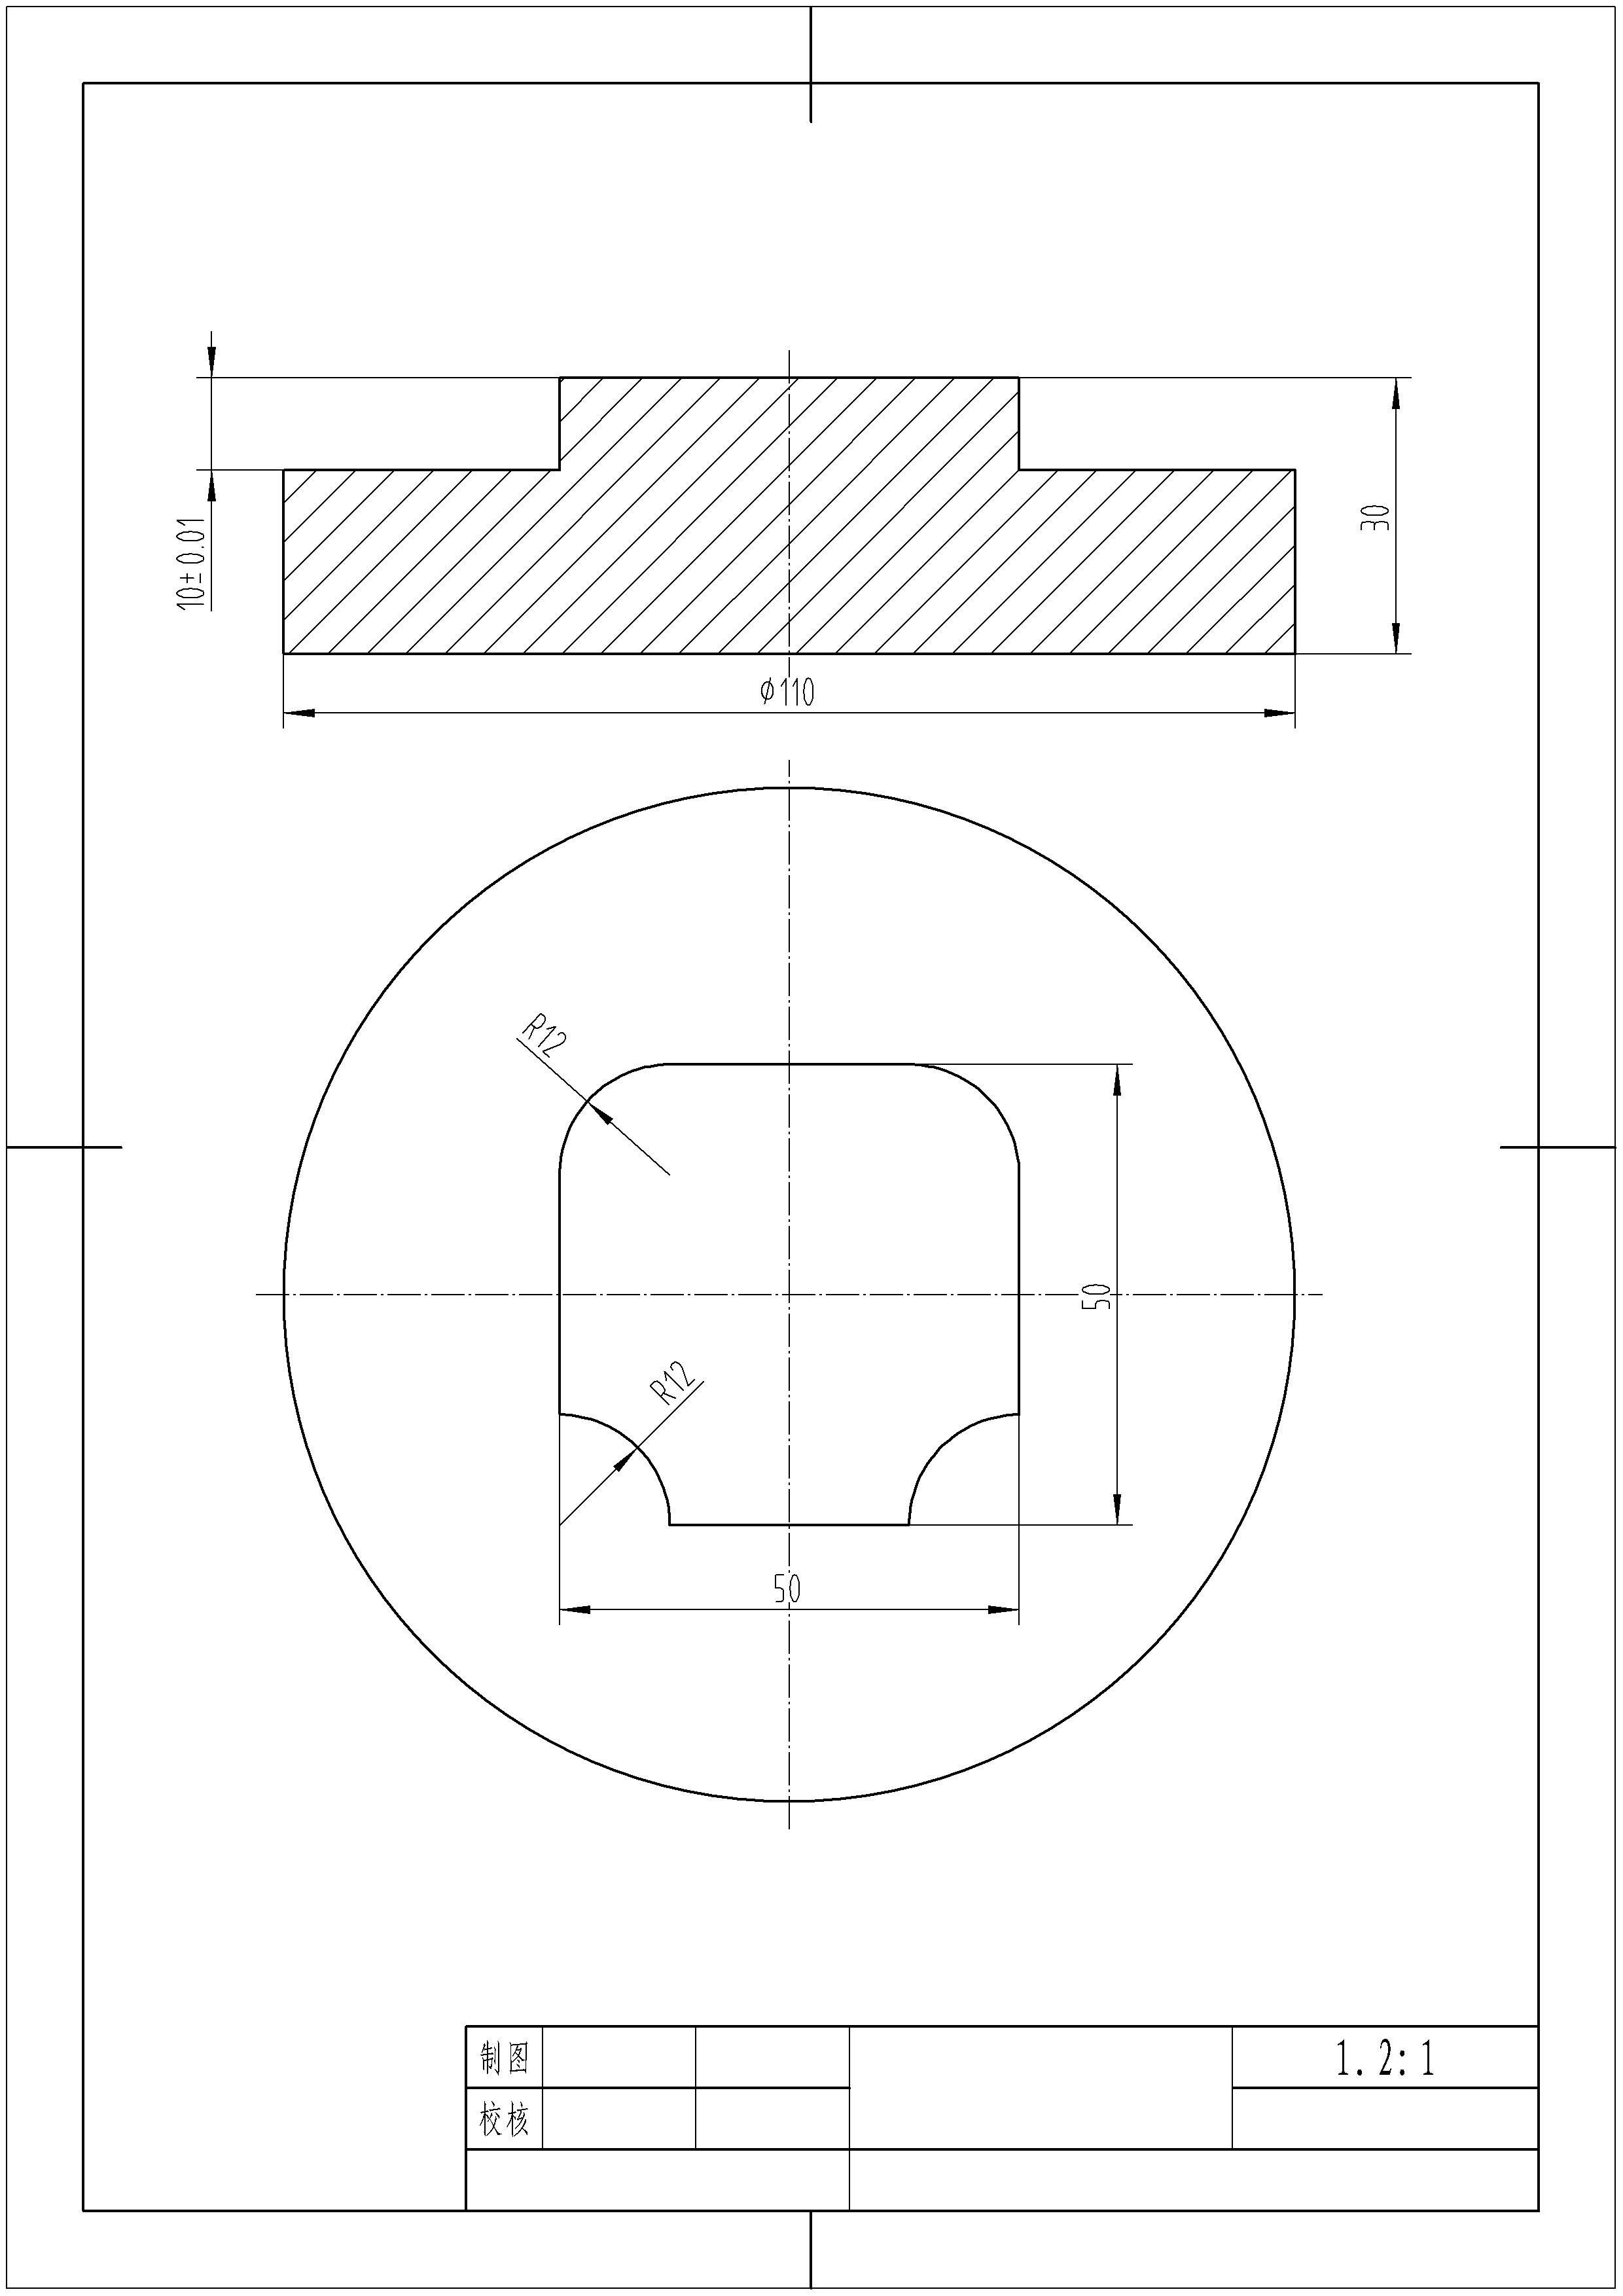
\includegraphics[width=0.8\linewidth,trim=50 150 50 100,clip]{data/image/5-1.jpg}
    \caption{}
    \label{fig:5-1}
\end{figure}

\begin{enumerate}[1、]
    \item 图样分析;
    \item 确定加工内容;
    \item 确定装夹及工件坐标系;
    \item 确定刀具及切削用量;
    \item 确定工序及走刀路线;
    \item 计算点坐标;
    \item 编写程序单。
\end{enumerate}

\subsection{教学内容及过程}

\subsubsection{案例分析}

在数控铣床或加工中心上加工如图\ref{fig:4-1}所示的零件,试完成程序的编写,已知毛坯为 $\Phi$ 110*30。

\begin{figure}[h]
    \centering
    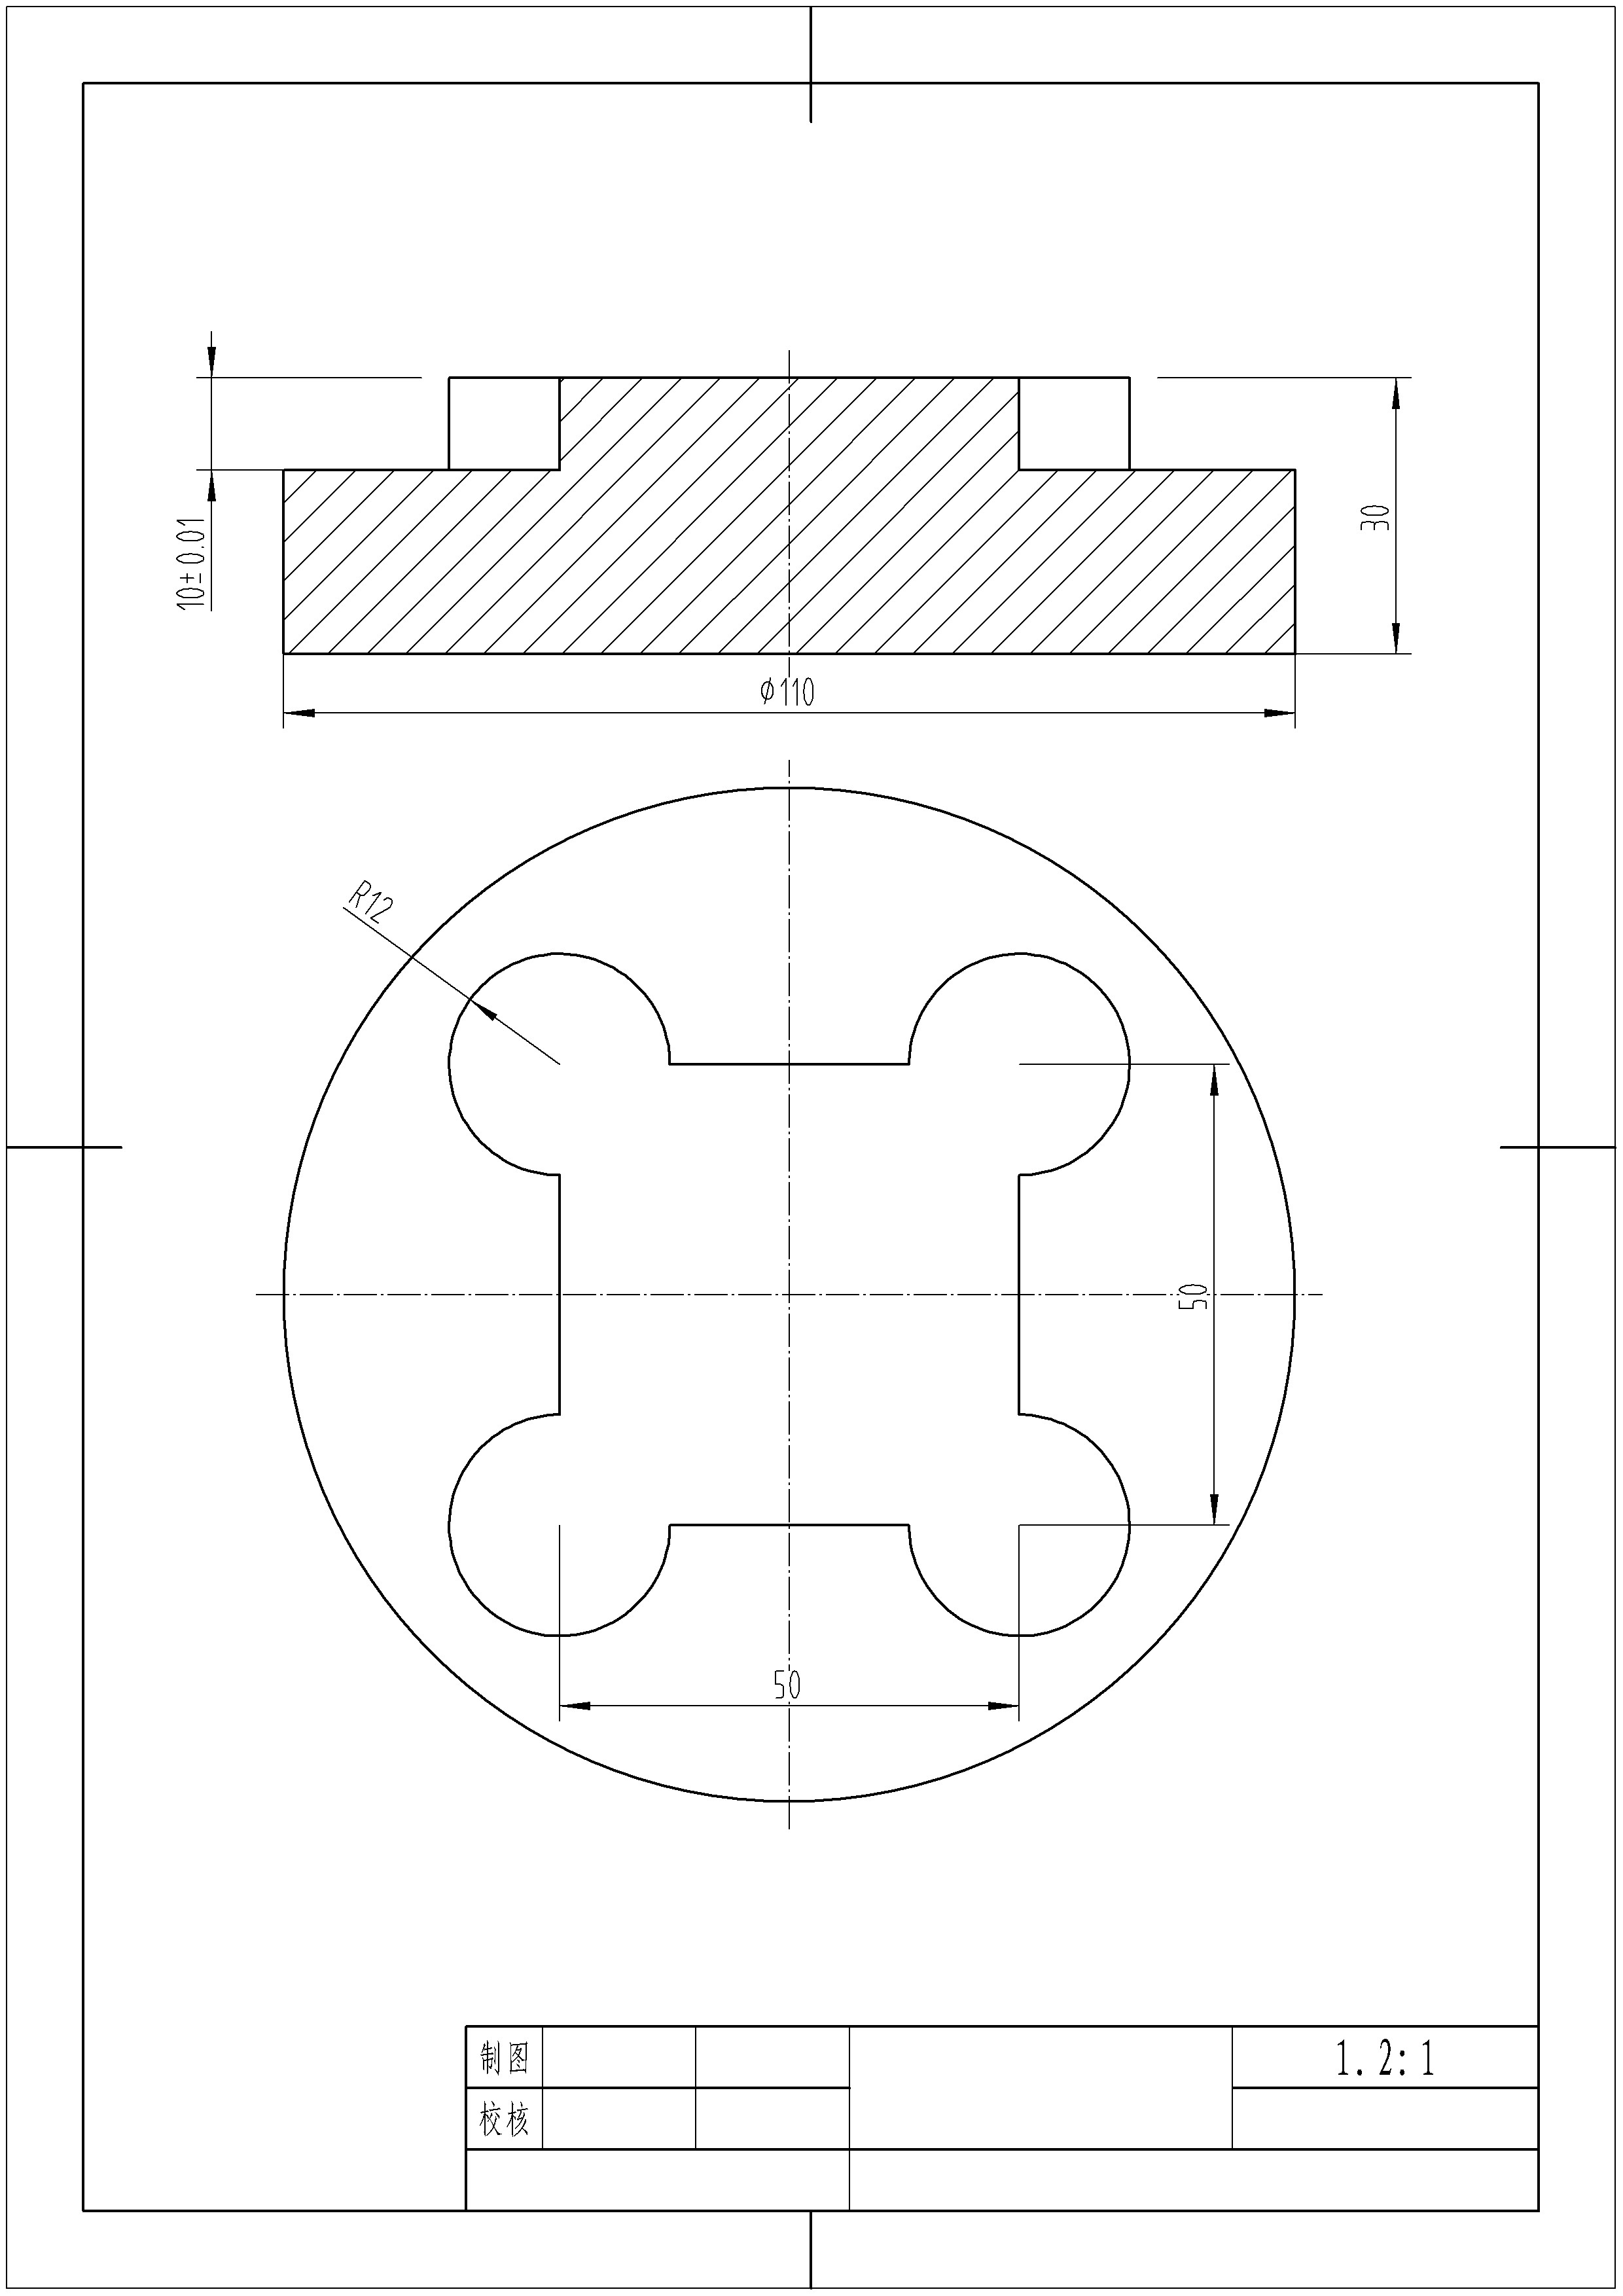
\includegraphics[width=0.8\linewidth,trim=50 150 50 100,clip]{data/image/5-2.jpg}
    \caption{}
    \label{fig:5-2}
\end{figure}

\begin{enumerate}[1、]
    \item 图样分析;
    \item 确定加工内容;
    \item 确定装夹及工件坐标系;
    \item 确定刀具及切削用量;
    \item 确定工序及走刀路线;
    \item 计算点坐标;
    \item 编写程序单。
\end{enumerate}


路径特点:

圆弧的圆心角大于180度,显然不能直接用前面的程序。

解决方法:解决方法:



1、把圆弧分成多个圆心角小于180度的圆弧。

2、掌握圆心角大于180度圆弧指令的使用。

当圆心角大于180度时,用负的半径值来表示。

当圆心角小于180度时,用正的半径值来表示。

Siemens上用CR= 正负规则一样。



\subsubsection{整圆编程}
在数控铣床或加工中心上用整圆的路径进行面铣,面铣深度为1mm,试完成加工成型的编写。
\begin{figure}[h]
    \centering
    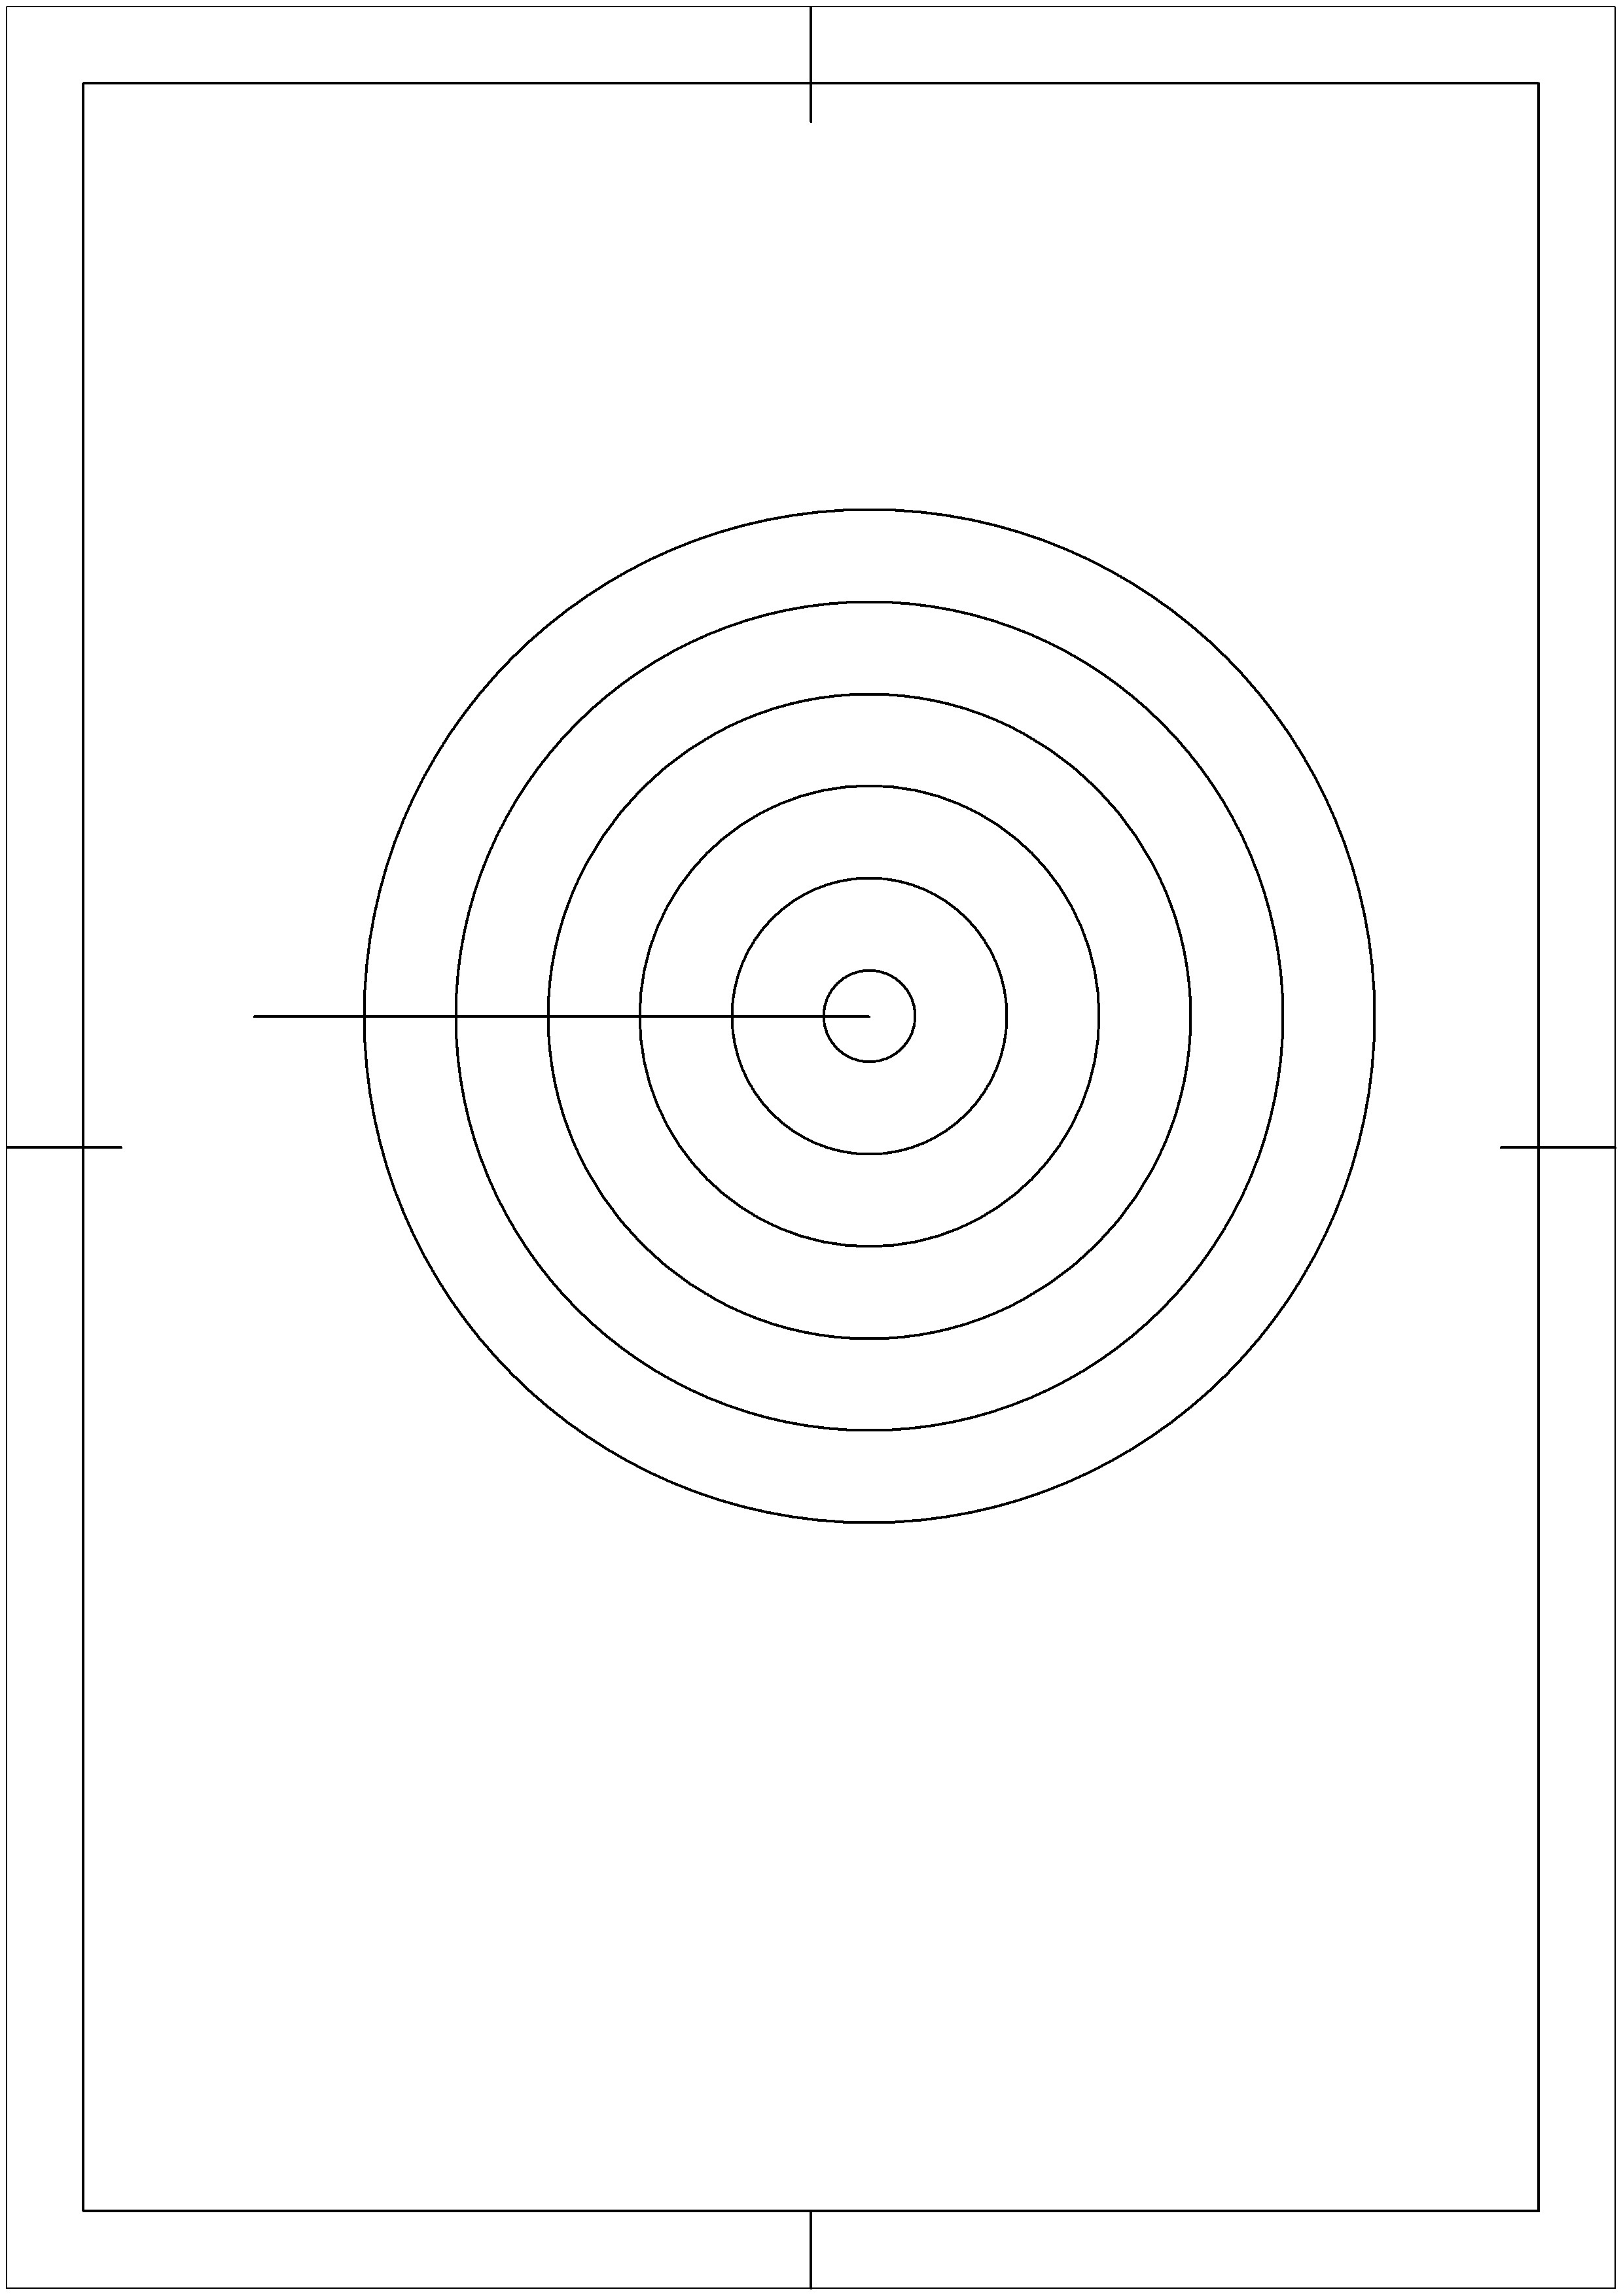
\includegraphics[width=0.8\linewidth,trim=50 150 50 100,clip]{data/image/5-3.jpg}
    \caption{}
    \label{fig:5-3}
\end{figure}

整圆路径也可以分成多个圆弧。

一个整圆路径可以用IJK圆心来编程。

不能用半径来编写一个整圆。


I、J、K表示圆心相对于起点的坐标。即:

I=X圆心-X起点

J=Y圆心-Y起点

K=Z圆心-Z起点

I、J、K与G90/G91无关,只与整圆的起点有关。

如: G17 G90 G2 X-50.0 Y-50.0 I50.0 J0;

参考程序:

\begin{lstlisting}
O0001;
G54G17G90;
M3S500;
G1Z30.0F2000;
X-65.Y0;
Z5.0;
Z-1.0F200;
X-55.0;
G2X-55.0Y0I55.0;
G1X-45.0;
G2I45.0;
G1X-35.0;
G2I-35.0;
G1X-25.0;
G2I-25.0;
G1X-15.0;
G2I-15.0;
G1X-5.0;
G2I5.0;
G1Z5.0;
Z30.0F2000;
M5;
M30;
\end{lstlisting}

\subsubsection{I、J、K的应用}
在数控铣床或加工中心上加工如图所示的零件,试用I、J、K完成程序的编写。
\begin{figure}[h]
    \centering
    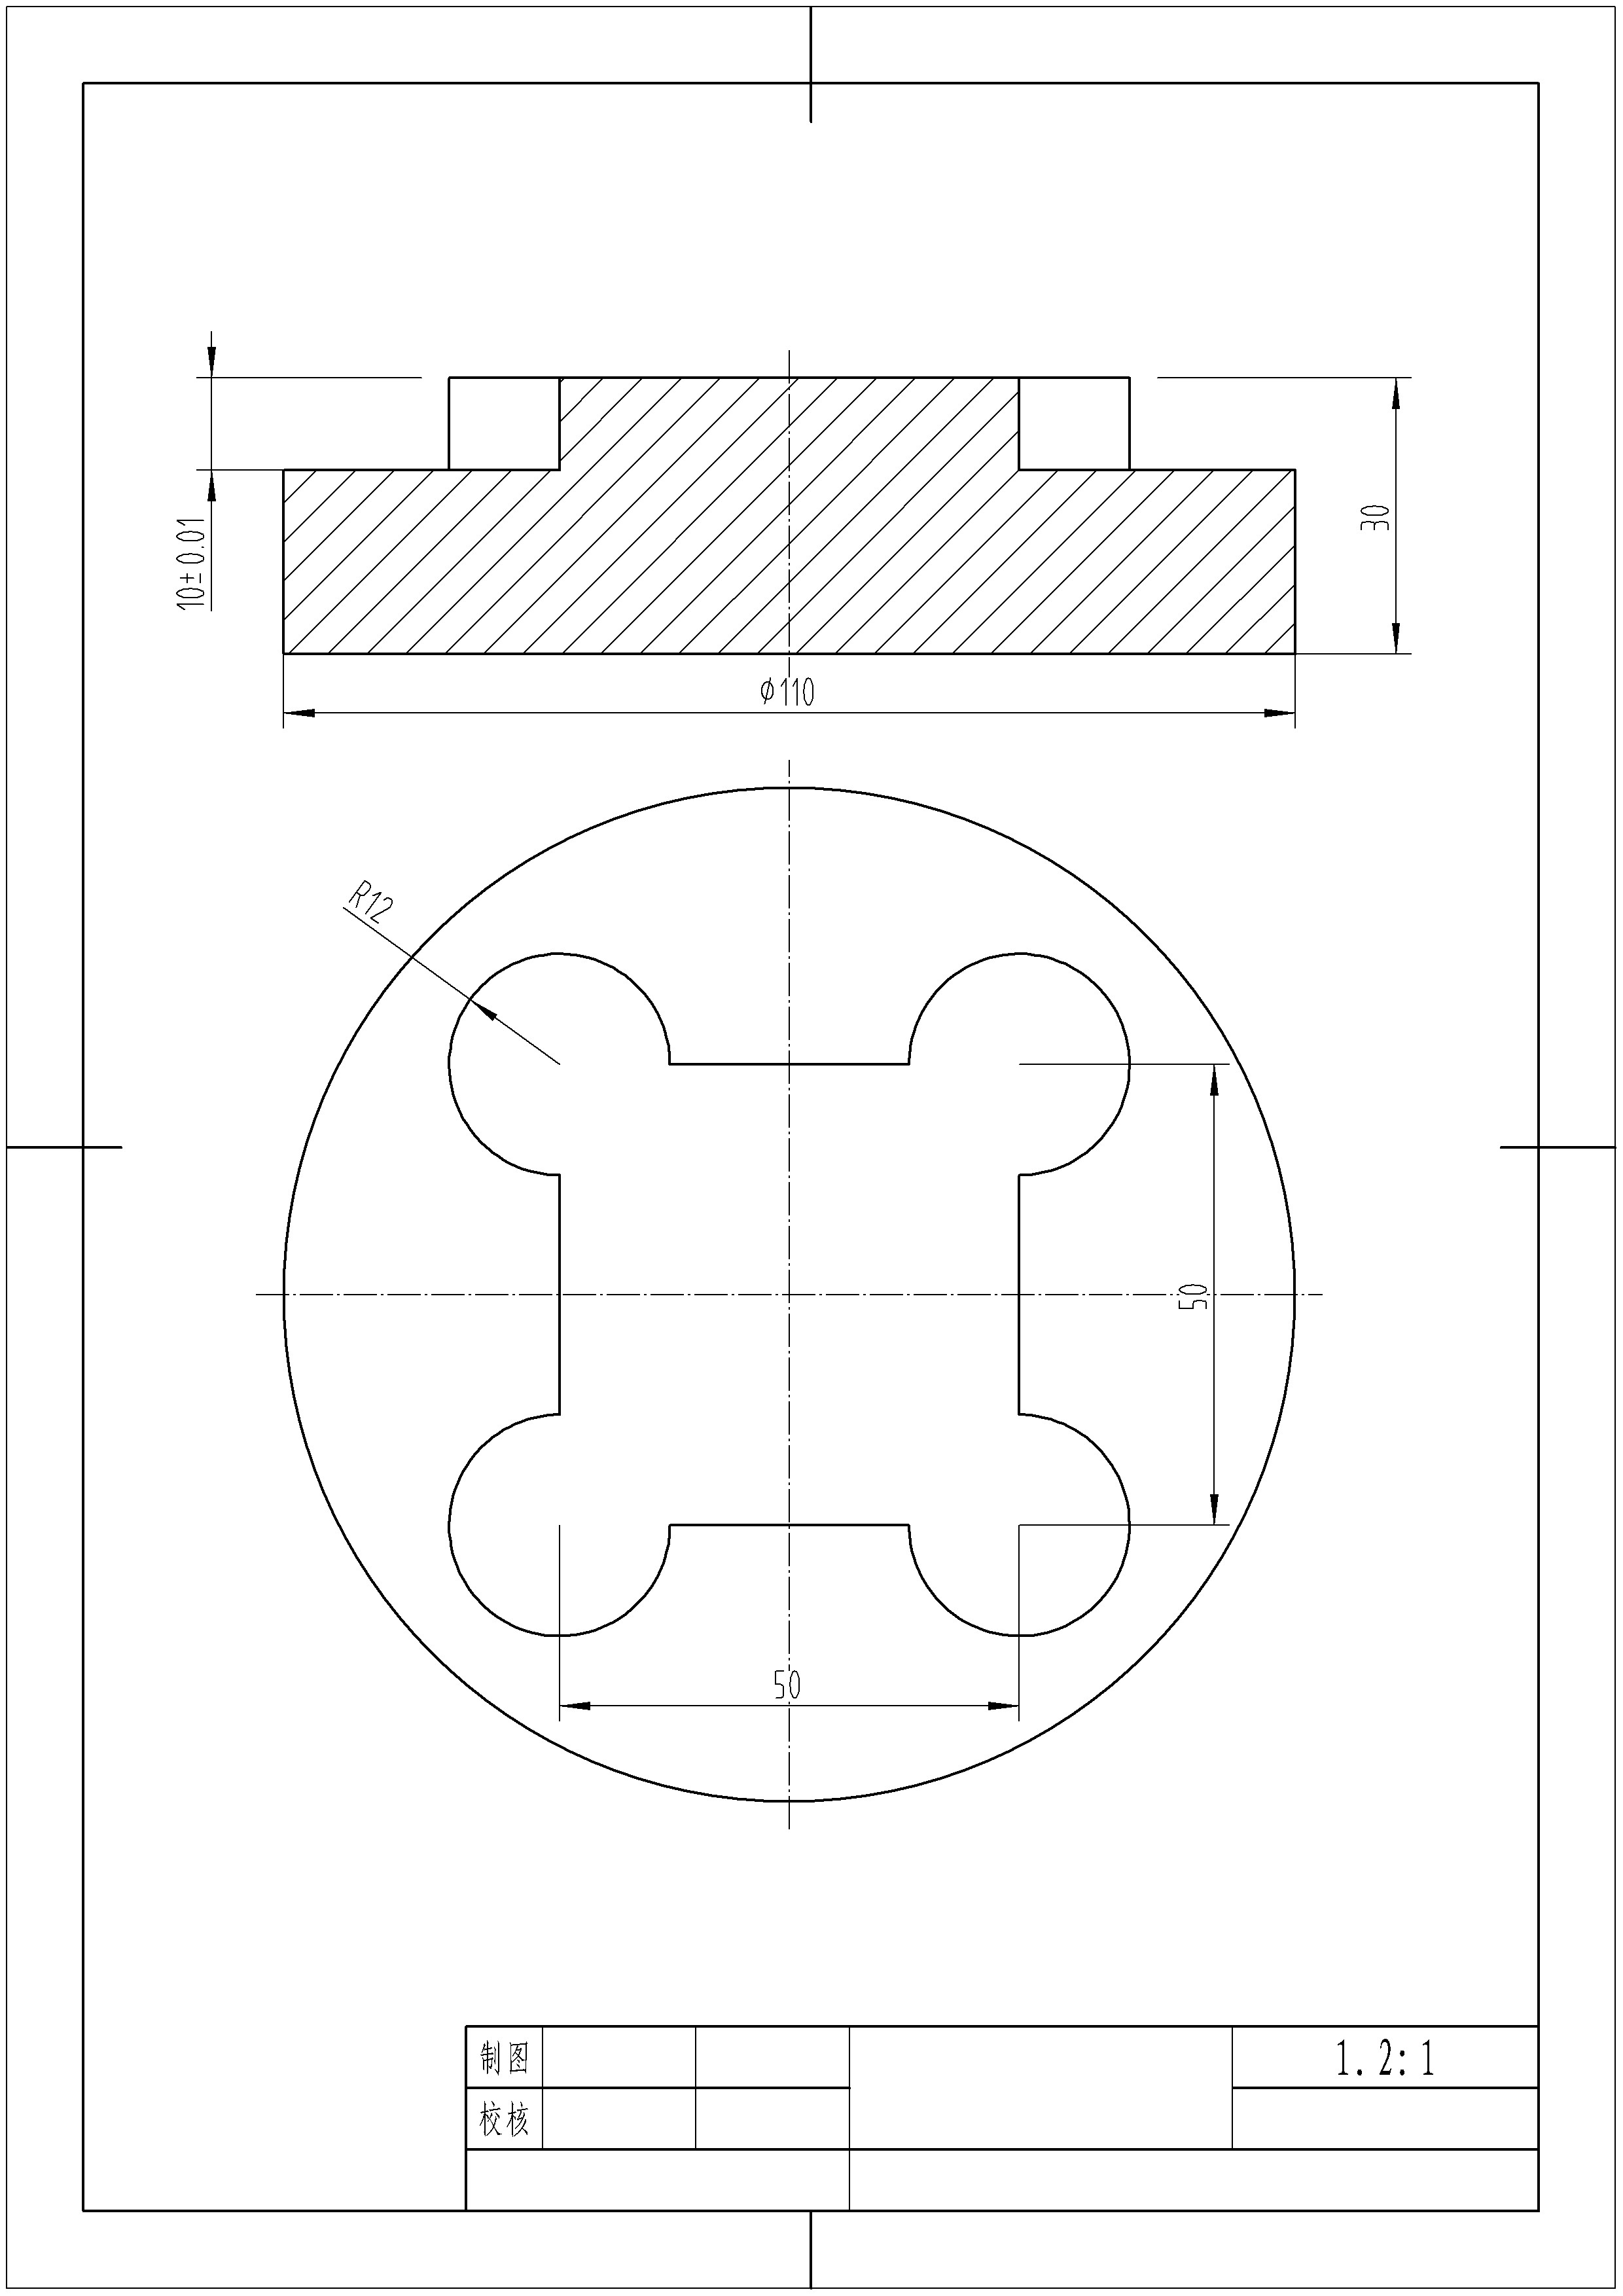
\includegraphics[width=0.8\linewidth,trim=50 150 50 100,clip]{data/image/5-4.jpg}
    \caption{}
    \label{fig:5-4}
\end{figure}
参考程序:

\begin{lstlisting}
O0001;
G54G17G90;
M3S500;
G1Z30.0F2000;
X-65.0Y0;
Z5.0;
Z-10.0F2000;
X-25.0;
Y13.0;
G2X-13.0Y25.0J13.0;
G1X13.0;
G2X25.0Y13.OJ-13.0;
….
\end{lstlisting}






手工编程中,能用半径编程就用半径编程,一般零件图标的是半径,也不容易出错。

自动编程,可以输出I、J、K以增加程序在不同机床通用性。


\subsubsection{编写程序的基本思路}
程序初始化(安全保护)--------辅助准备(换刀,主轴启动,切削液开)--------定位到起刀点--------快速下刀--------工进下刀--------走加工轮廓--------提刀---------快速提刀到安全平面-------程序结束(换刀,主轴停止,切削液关,程序返回等)
\subsection{课堂小结}
\begin{enumerate}[1、]
\item 案例分析;
\item 指令讲解;
\item 编写程序;
\item 编写程序的基本思路。
\end{enumerate}
\vfill
\subsection{布置作业}
\begin{enumerate}[1、]
	\item 自定尺寸,编写加工一个矩形外形的程序?
\end{enumerate}
\vfill
\jxhj{%教学后记
}
\skrq{%授课日期
	2017年9月26日 4-5节}
\ktmq{%课题名称
	基本指令(三) }
\jxmb{%教学目标,每行前面要加 \item
	\item 掌握G2/G3半径-R的使用;
	\item 掌握G2/G3圆心编程的使用;
	\item 能用G2/G3进行程序的编写;
	\item 掌握编写数控程序的基本思路。}
\jxzd{%教学重点,每行前面要加 \item
	\item G2/G3半径-R的使用;
	\item G2/G3圆心编程的使用;}
\jxnd{%教学难点,每行前面要加 \item
	\item G2/G3圆心编程的使用;}
\jjff{%教学方法
	通过讲述、举例、演示法来说明;}

\makeshouye %制作教案首页

%%%%教学内容
\subsection{组织教学}
\begin{enumerate}[1、]
	\item 集中学生注意力;
	\item 清查学生人数;
	\item 维持课堂纪律;
\end{enumerate}
\subsection{复习导入及主要内容}
\begin{enumerate}[1、]
	\item 案例分析;
	\item 指令讲解G2/G3;
	\item 编写程序;
	\item 编写程序的基本思路。
\end{enumerate}

\textbf{案例分析}

在数控铣床或加工中心上加工如图\ref{fig:6-1}所示的零件,试完成程序的编写,已知毛坯为 $\Phi$ 110*30。

\begin{figure}[h]
	\centering
	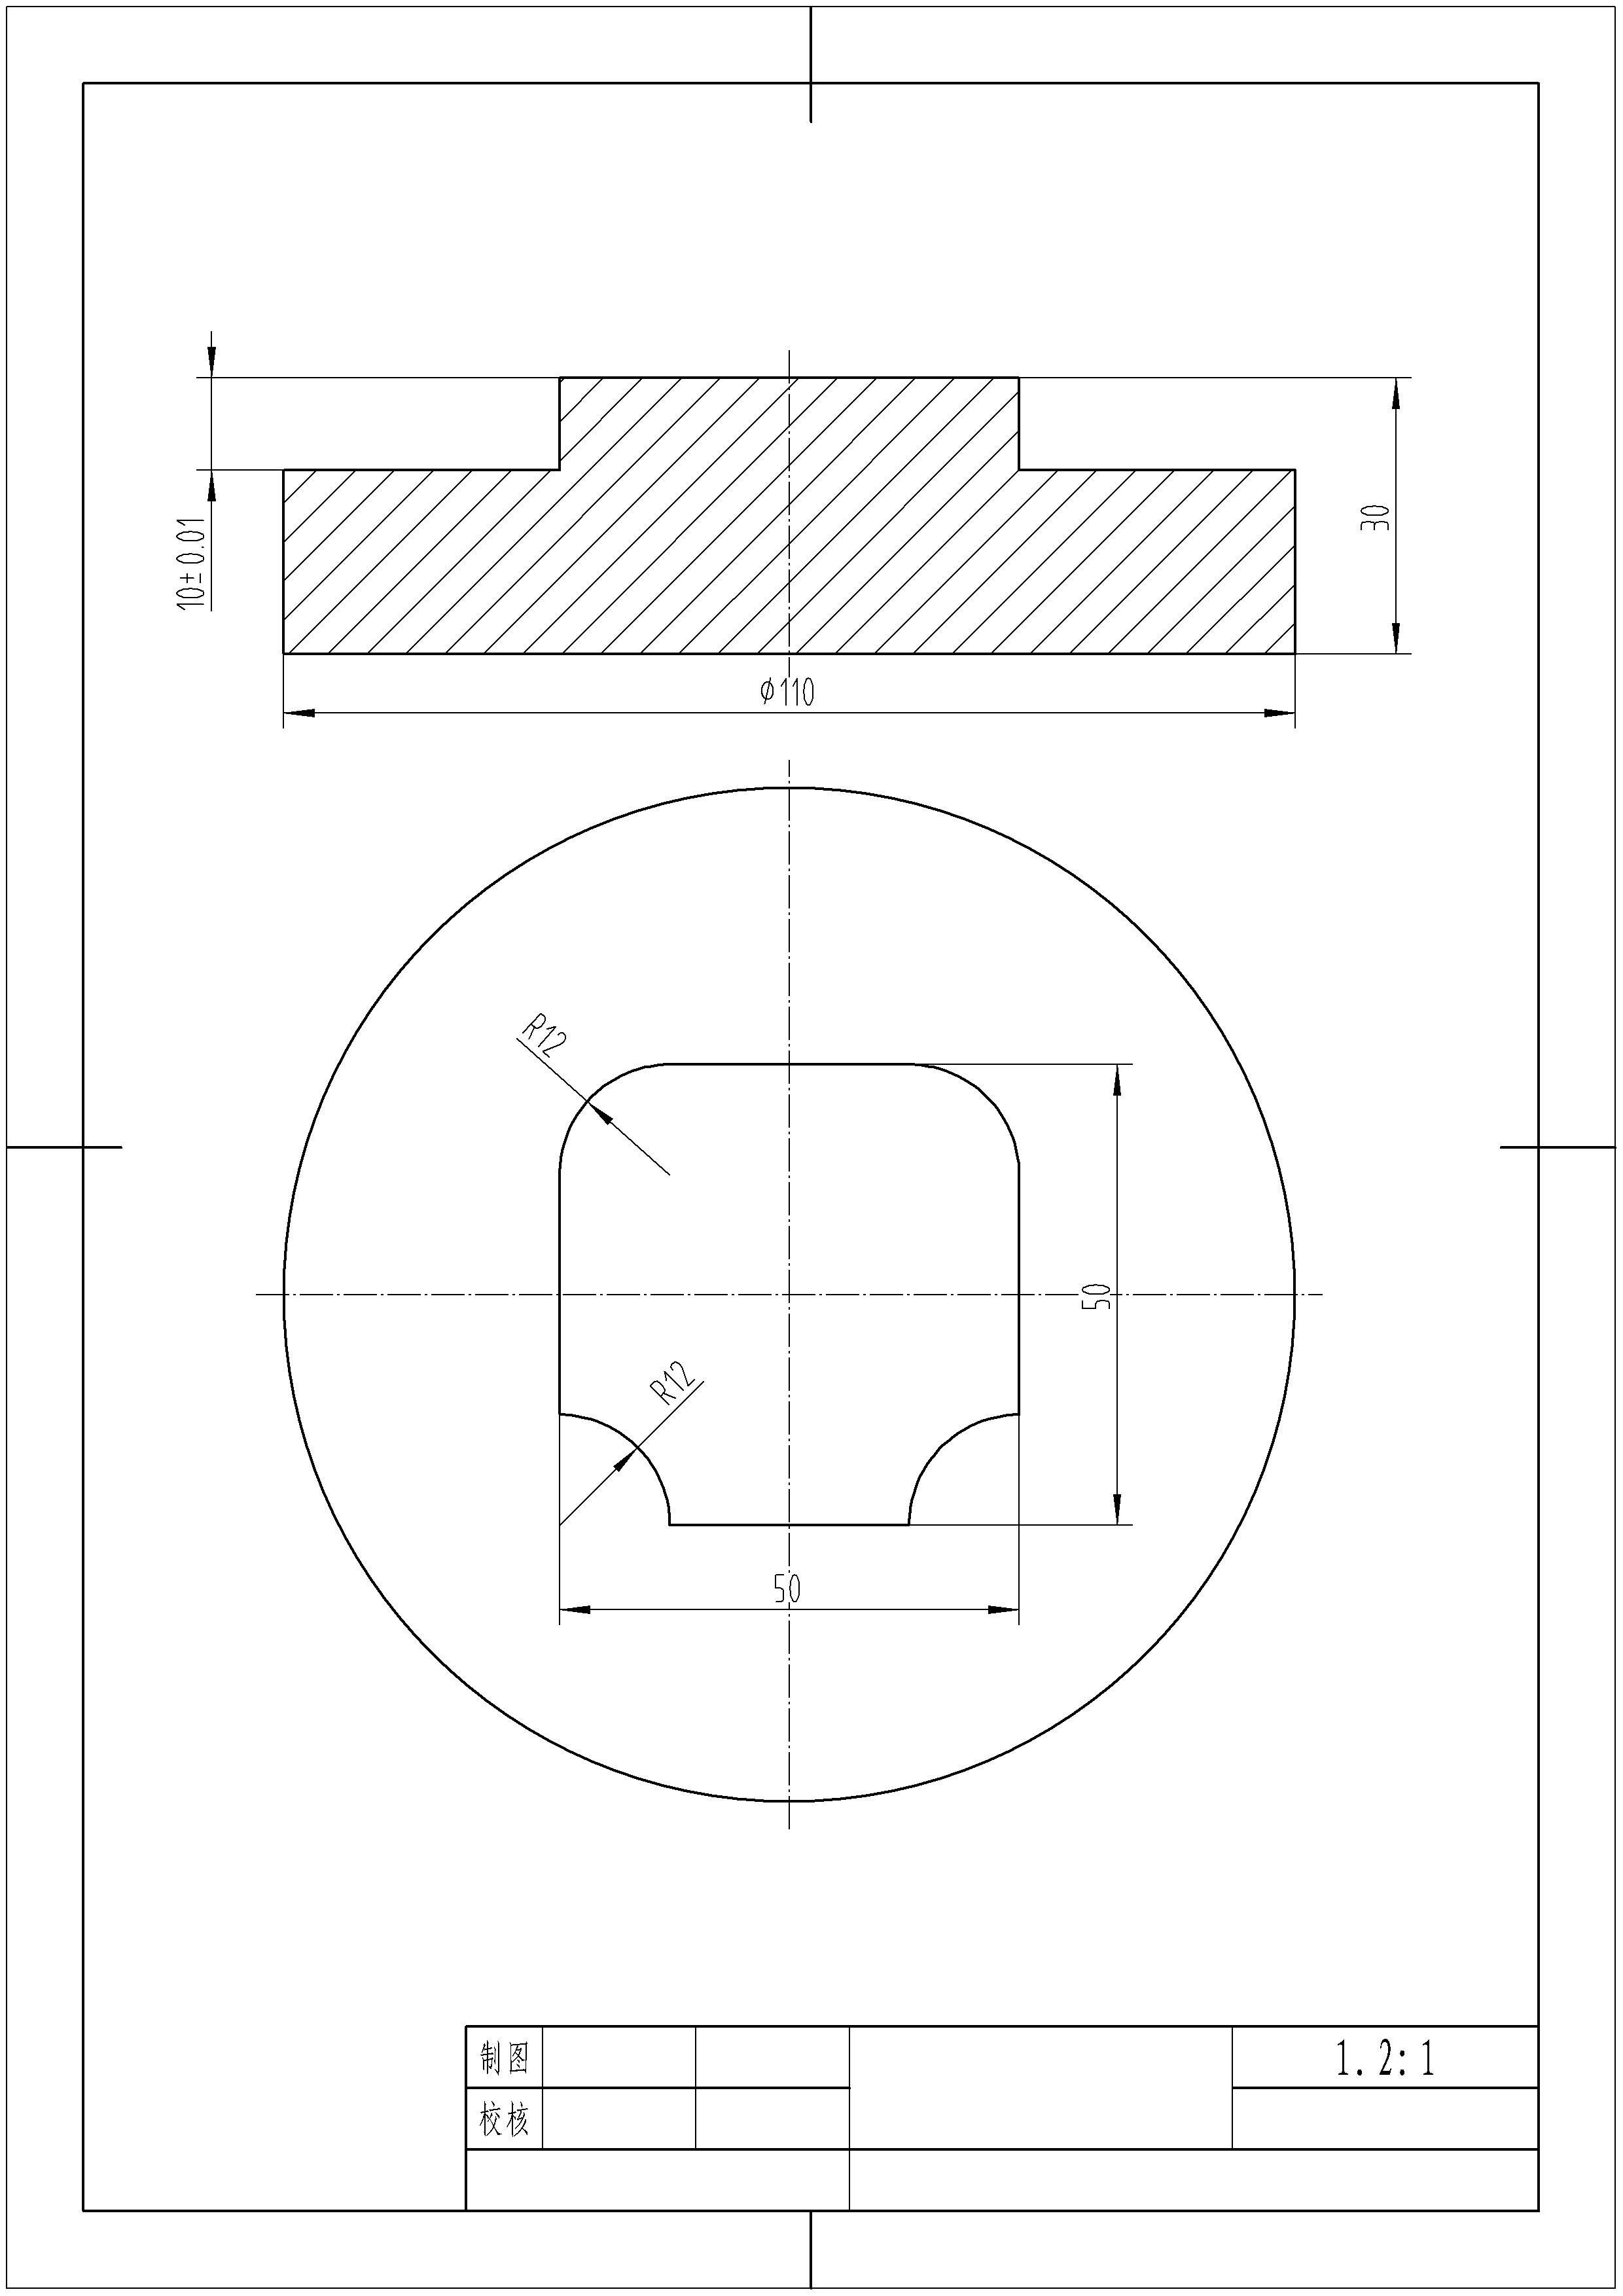
\includegraphics[width=0.8\linewidth,trim=50 150 50 100,clip]{data/image/5-1.jpg}
	\caption{}
	\label{fig:6-1}
\end{figure}

\begin{enumerate}[1、]
	\item 图样分析;
	\item 确定加工内容;
	\item 确定装夹及工件坐标系;
	\item 确定刀具及切削用量;
	\item 确定工序及走刀路线;
	\item 计算点坐标;
	\item 编写程序单。
\end{enumerate}

\subsection{教学内容及过程}

\subsubsection{案例分析}

在数控铣床或加工中心上加工如图\ref{fig:6-2}所示的零件,试完成程序的编写,已知毛坯为 $\Phi$ 110*30。

\begin{figure}[h]
	\centering
	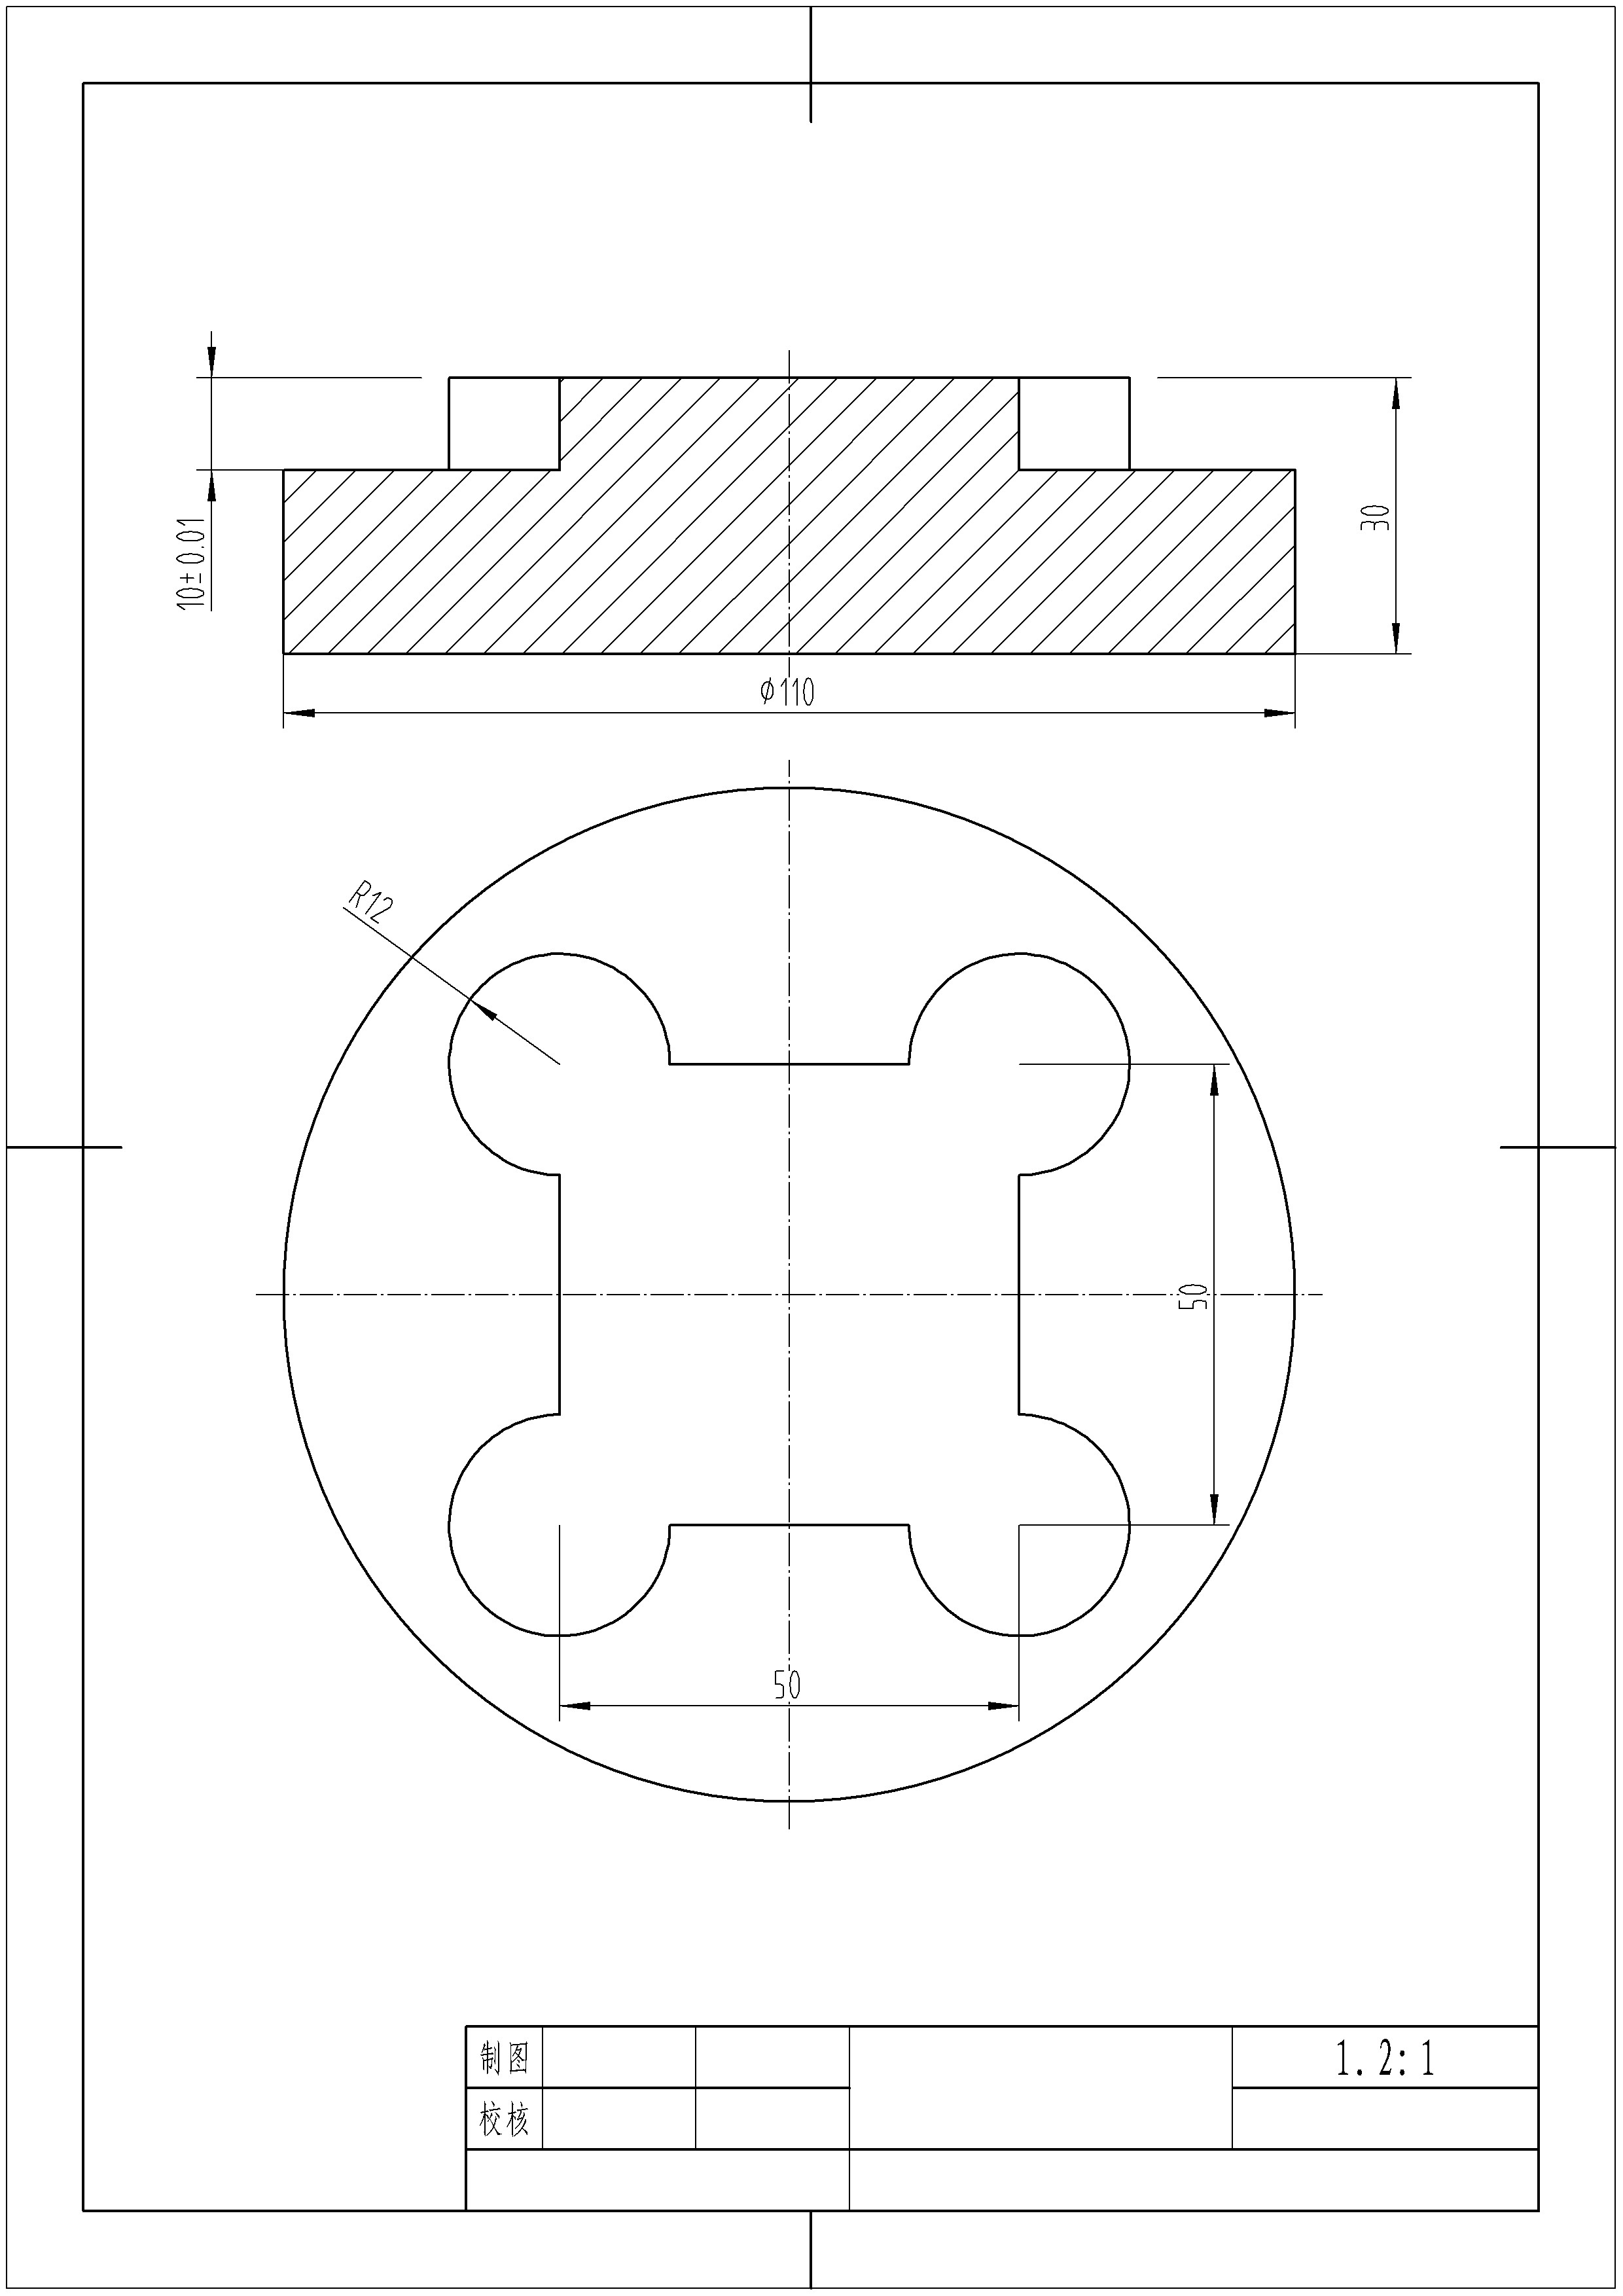
\includegraphics[width=0.8\linewidth,trim=50 150 50 100,clip]{data/image/5-2.jpg}
	\caption{}
	\label{fig:6-2}
\end{figure}

\begin{enumerate}[1、]
	\item 图样分析;
	\item 确定加工内容;
	\item 确定装夹及工件坐标系;
	\item 确定刀具及切削用量;
	\item 确定工序及走刀路线;
	\item 计算点坐标;
	\item 编写程序单。
\end{enumerate}


路径特点:

圆弧的圆心角大于180度,显然不能直接用前面的程序。

解决方法:解决方法:



1、把圆弧分成多个圆心角小于180度的圆弧。

2、掌握圆心角大于180度圆弧指令的使用。

当圆心角大于180度时,用负的半径值来表示。

当圆心角小于180度时,用正的半径值来表示。

Siemens上用CR= 正负规则一样。



\subsubsection{整圆编程}
在数控铣床或加工中心上用整圆的路径进行面铣,面铣深度为1mm,试完成加工成型的编写。
\begin{figure}[h]
	\centering
	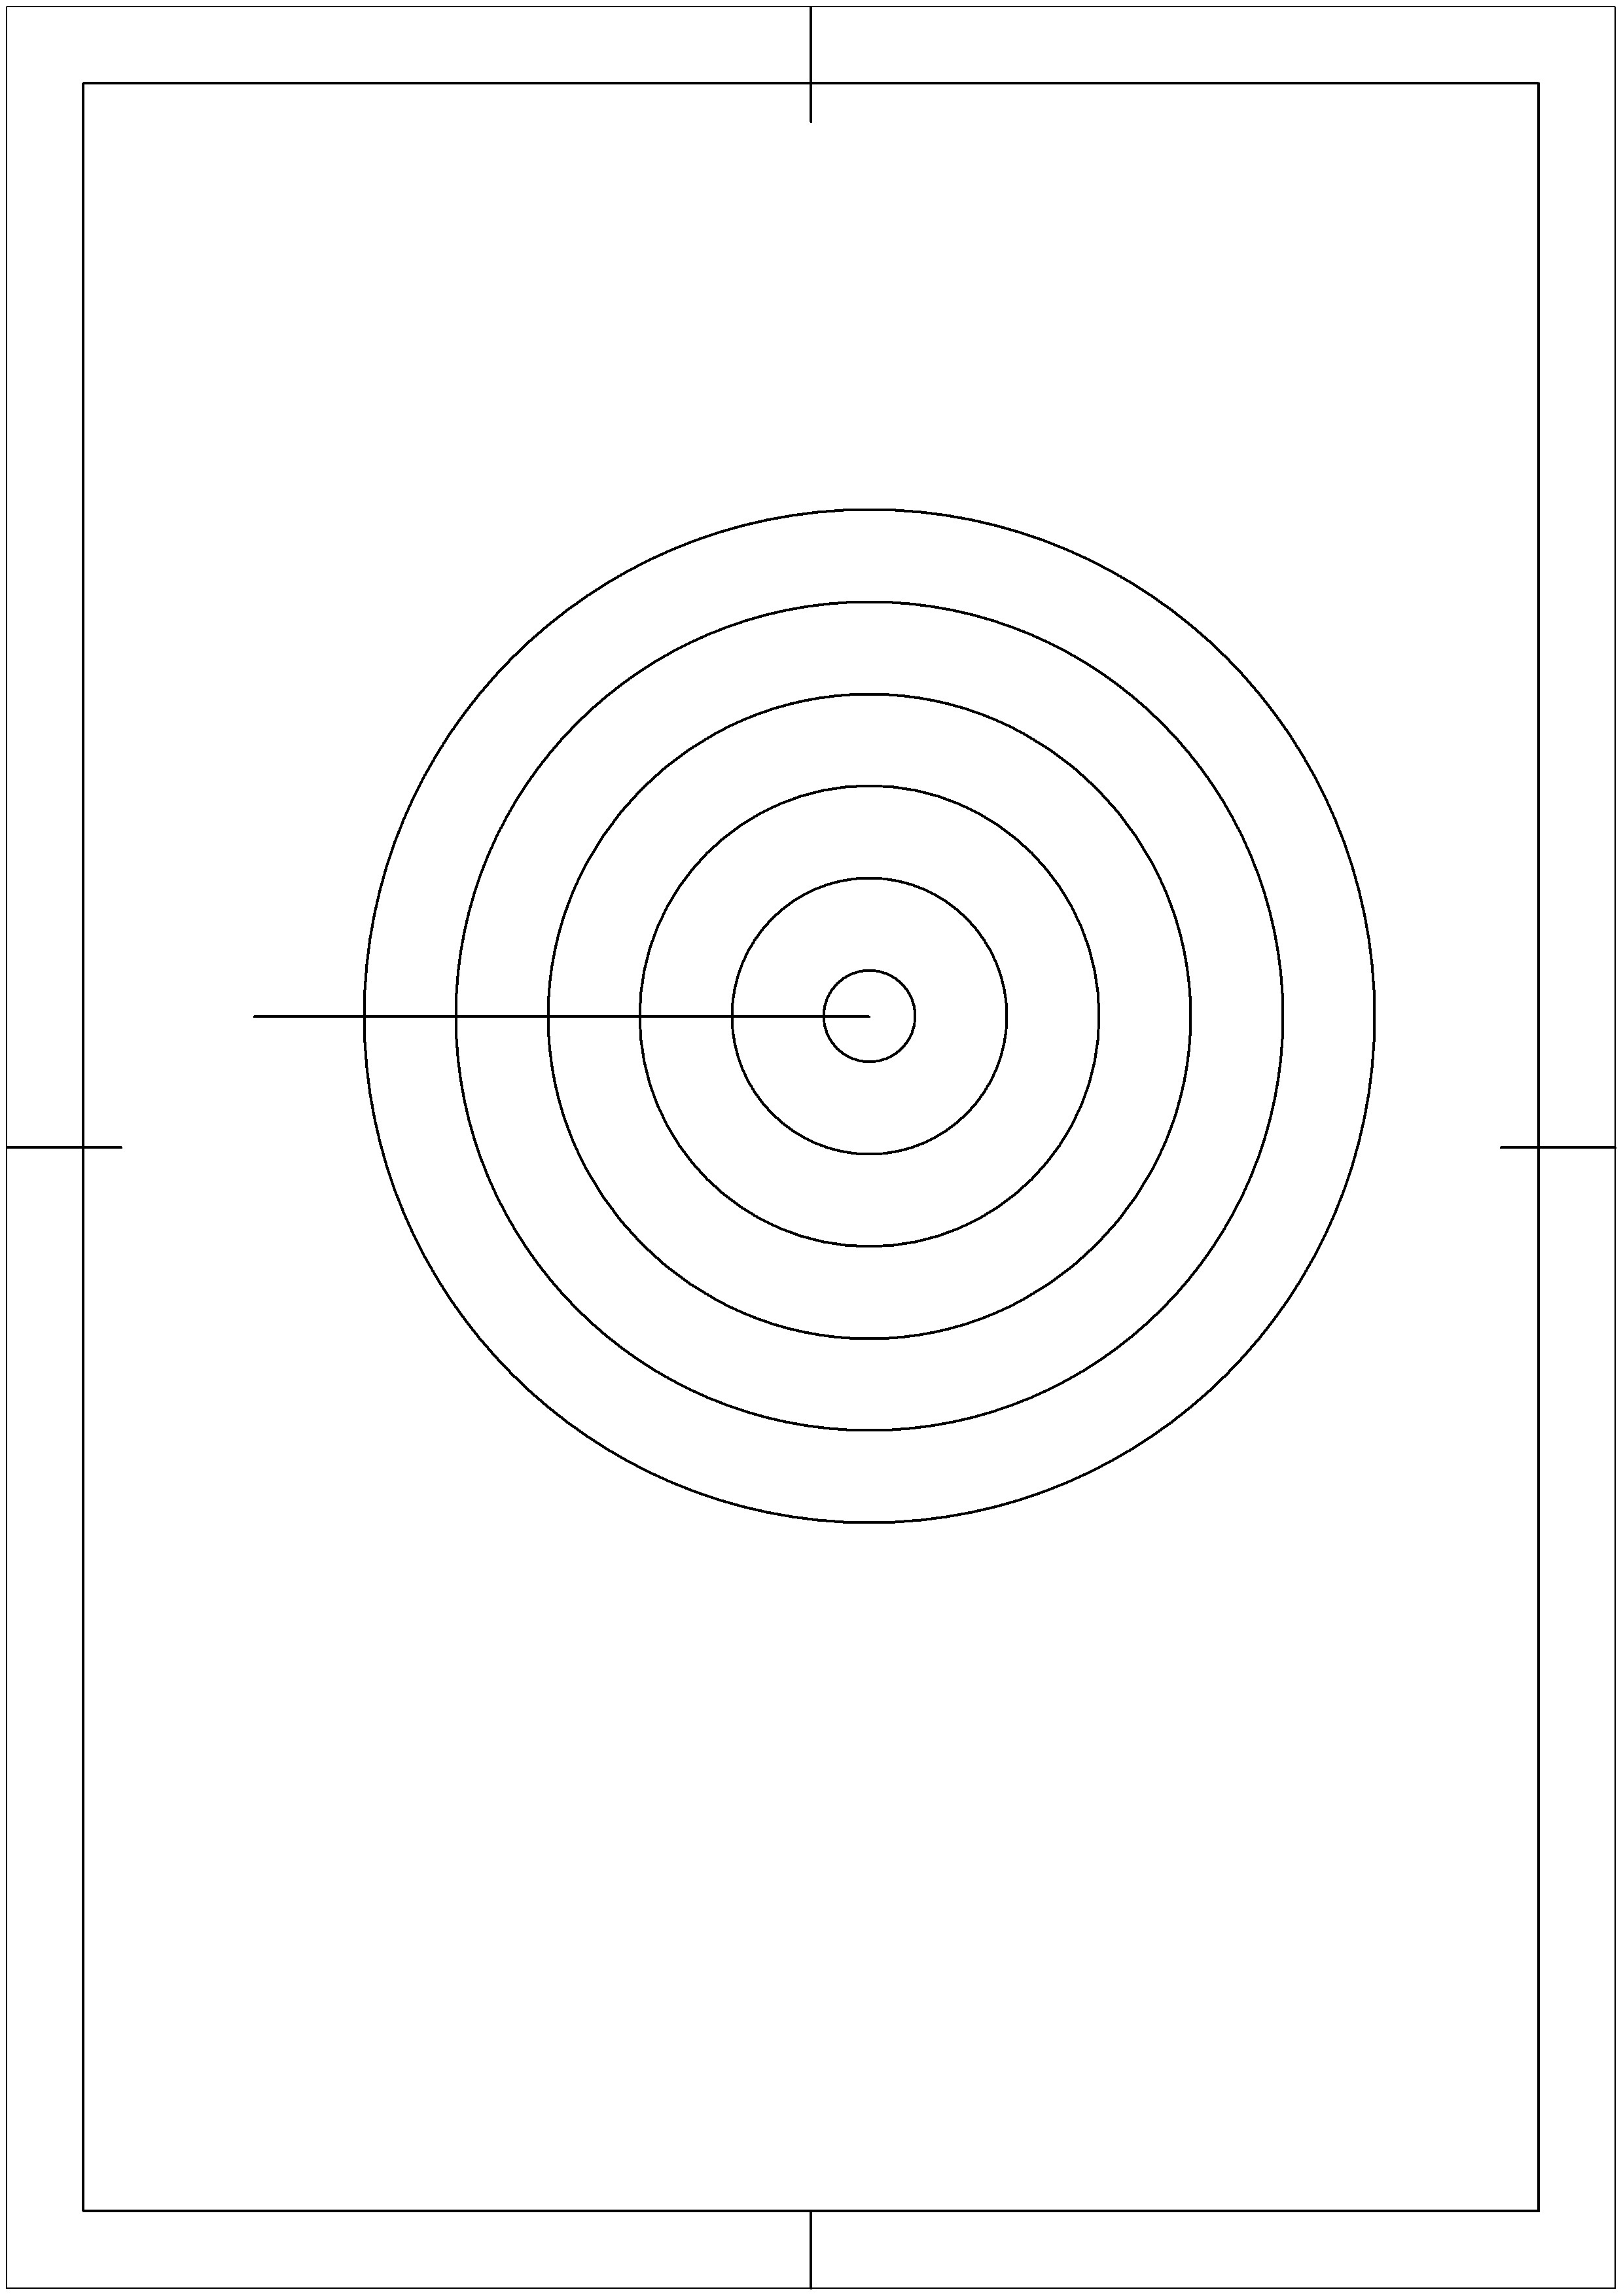
\includegraphics[width=0.8\linewidth,trim=50 150 50 100,clip]{data/image/5-3.jpg}
	\caption{}
	\label{fig:6-3}
\end{figure}

整圆路径也可以分成多个圆弧。

一个整圆路径可以用IJK圆心来编程。

不能用半径来编写一个整圆。


I、J、K表示圆心相对于起点的坐标。即:

I=X圆心-X起点

J=Y圆心-Y起点

K=Z圆心-Z起点

I、J、K与G90/G91无关,只与整圆的起点有关。

如: G17 G90 G2 X-50.0 Y-50.0 I50.0 J0;

参考程序:

\begin{lstlisting}
O0001;
G54G17G90;
M3S500;
G1Z30.0F2000;
X-65.Y0;
Z5.0;
Z-1.0F200;
X-55.0;
G2X-55.0Y0I55.0;
G1X-45.0;
G2I45.0;
G1X-35.0;
G2I-35.0;
G1X-25.0;
G2I-25.0;
G1X-15.0;
G2I-15.0;
G1X-5.0;
G2I5.0;
G1Z5.0;
Z30.0F2000;
M5;
M30;
\end{lstlisting}

\subsubsection{I、J、K的应用}
在数控铣床或加工中心上加工如图所示的零件,试用I、J、K完成程序的编写。
\begin{figure}[h]
	\centering
	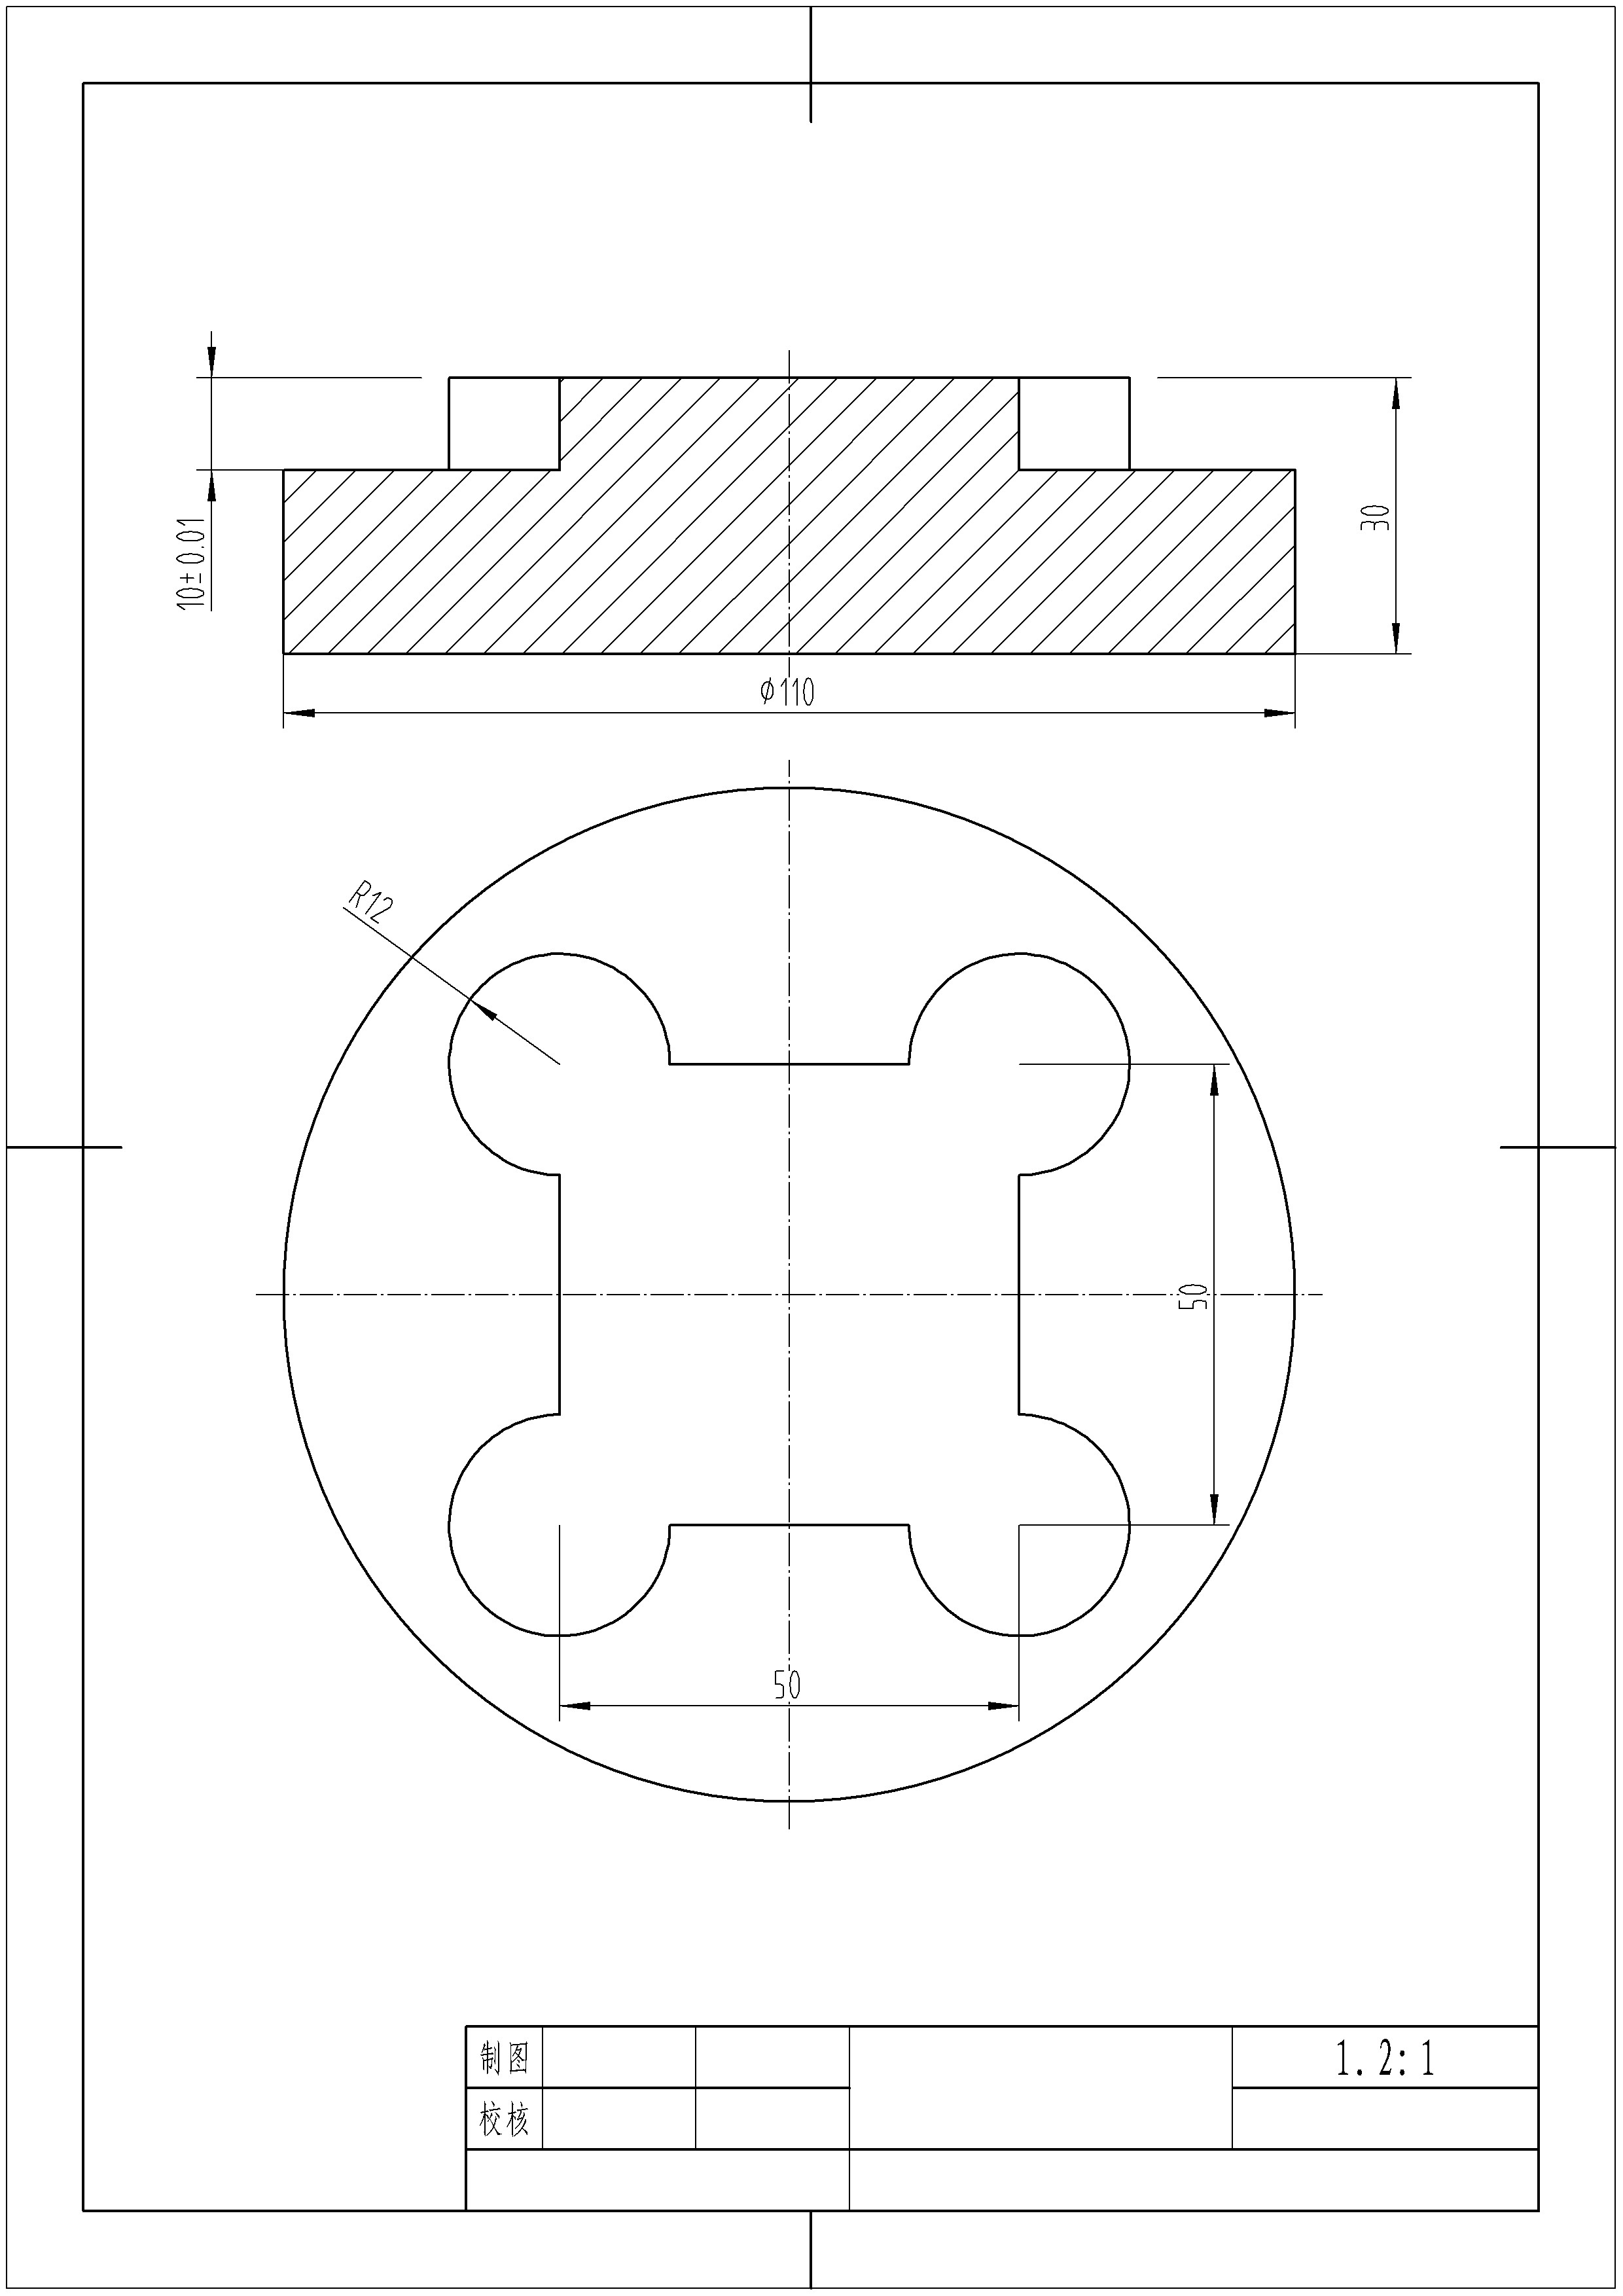
\includegraphics[width=0.8\linewidth,trim=50 150 50 100,clip]{data/image/5-4.jpg}
	\caption{}
	\label{fig:6-4}
\end{figure}
参考程序:

\begin{lstlisting}
O0001;
G54G17G90;
M3S500;
G1Z30.0F2000;
X-65.0Y0;
Z5.0;
Z-10.0F2000;
X-25.0;
Y13.0;
G2X-13.0Y25.0J13.0;
G1X13.0;
G2X25.0Y13.OJ-13.0;
….
\end{lstlisting}






手工编程中,能用半径编程就用半径编程,一般零件图标的是半径,也不容易出错。

自动编程,可以输出I、J、K以增加程序在不同机床通用性。


\subsubsection{编写程序的基本思路}
程序初始化(安全保护)--------辅助准备(换刀,主轴启动,切削液开)--------定位到起刀点--------快速下刀--------工进下刀--------走加工轮廓--------提刀---------快速提刀到安全平面-------程序结束(换刀,主轴停止,切削液关,程序返回等)
\subsection{课堂小结}
\begin{enumerate}[1、]
	\item 案例分析;
	\item 指令讲解;
	\item 编写程序;
	\item 编写程序的基本思路。
\end{enumerate}
\vfill
\subsection{布置作业}
\begin{enumerate}[1、]
	\item 自定尺寸,编写加工一个矩形外形的程序?
\end{enumerate}
\vfill
\jxhj{%教学后记
	}
\skrq{%授课日期
	2017年9月28日 4-5节}
\ktmq{%课题名称
	刀具半径补偿 }
\jxmb{%教学目标,每行前面要加 \item
	\item 了解补偿的意义;
	\item 掌握G41/G42刀具半径补偿指令的使用;
	\item 会用G41/G42刀具半径指令编写程序;
	\item 了解常用切入切出的方法。
}
\jxzd{%教学重点,每行前面要加 \item
	\item 掌握G41/G42刀具半径补偿指令的使用;
	\item 会用G41/G42刀具半径指令编写程序;}
\jxnd{%教学难点,每行前面要加 \item
	\item 会用G41/G42刀具半径指令编写程序;}
\jjff{%教学方法
	通过讲述、举例、演示法来说明;}

\makeshouye %制作教案首页

%%%%教学内容
\subsection{组织教学}
\begin{enumerate}[1、]
	\item 集中学生注意力;
	\item 清查学生人数;
	\item 维持课堂纪律;
\end{enumerate}
\subsection{复习导入及主要内容}
\begin{enumerate}[1、]
\item 在数控铣床或加工中心上加工如图所示的零件,试完成程序的编写。(试用I、J、K编写,凸台高5mm)

\begin{figure}[h]
	\centering
	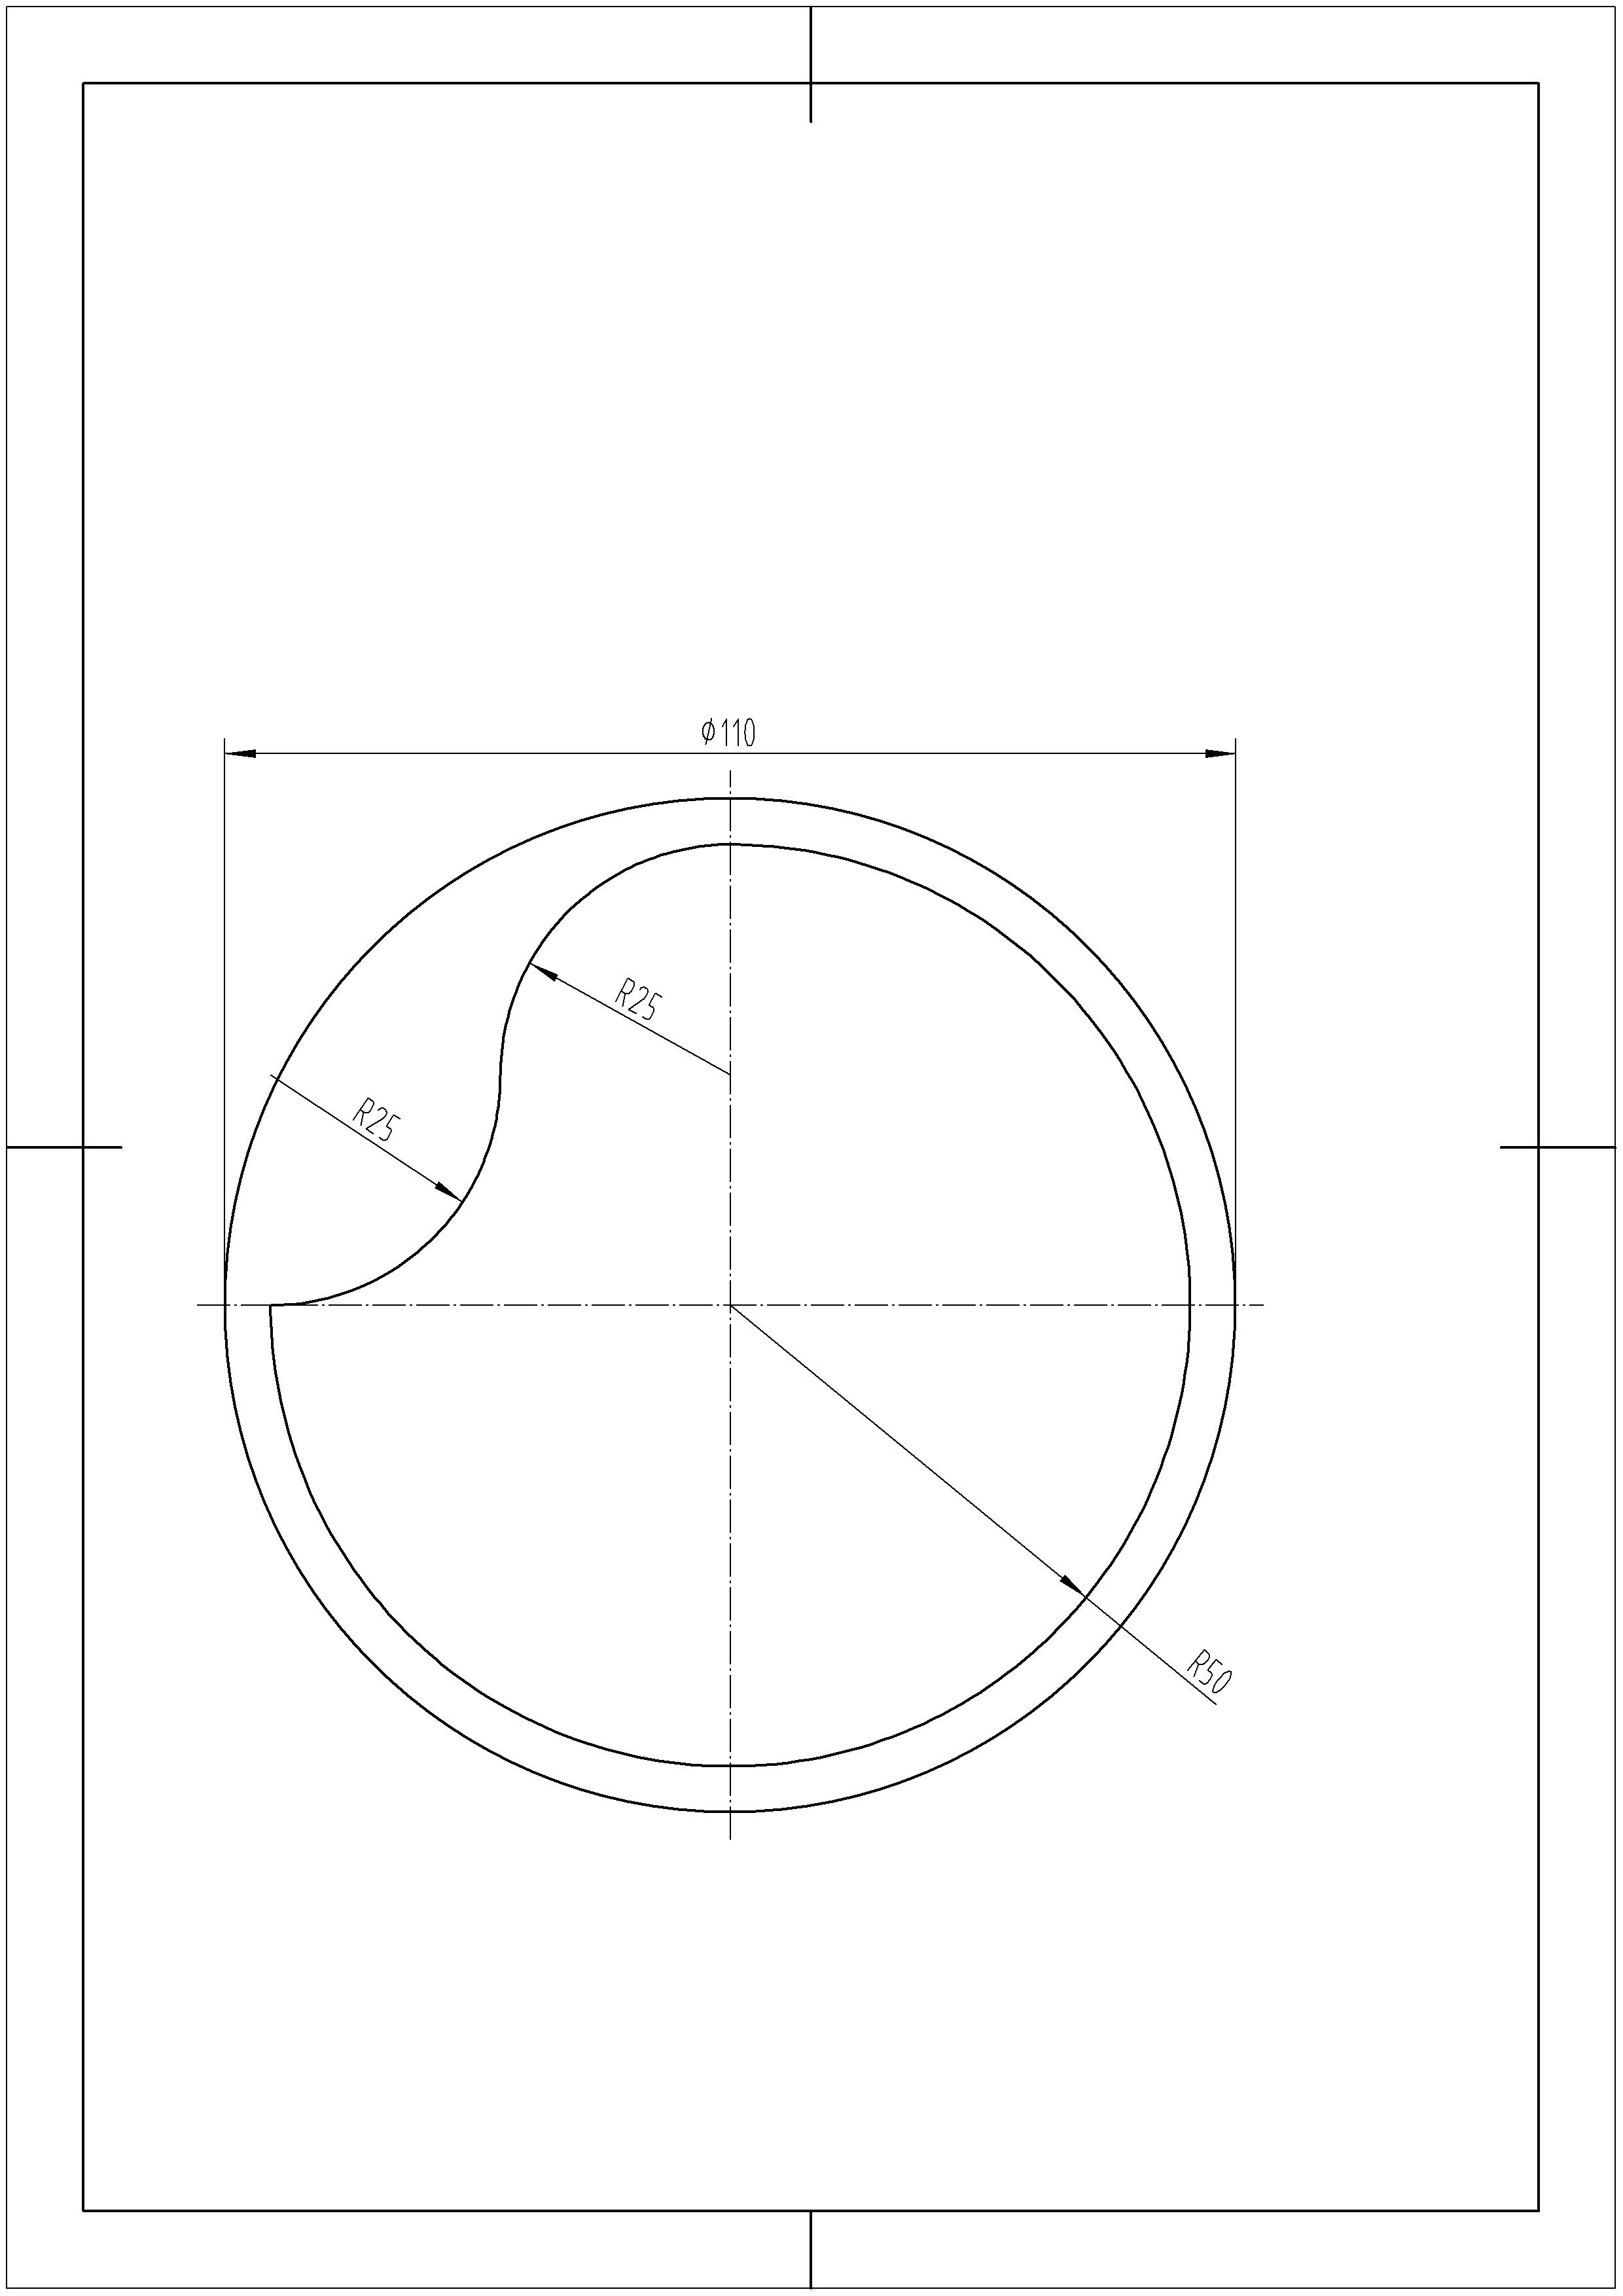
\includegraphics[width=0.8\linewidth,trim=40 150 70 220,clip]{data/image/7-1.jpg}
	\caption{复习题}
	\label{fig:7-1}
\end{figure}

\item G2/G3指令半径编程;
\item G2/G3指令圆心编程;
\item 编写程序的基本思路。
\end{enumerate}

\subsection{教学内容及过程}

\subsubsection{加工尺寸的分析}

由于加工刀具存在一个尺寸,故加工出来的尺寸值会每边少一个刀具半径。

解决方法:

1、更改加工刀路,使其偏移一个刀具半径(粗加工及去残料)。

2、使用刀具半径补偿指令进行编程。

例子:

\begin{lstlisting}
O0001;
G54G71G40G90;
M3S500;
G1Z30.F200O;
X70.YO;
Z5.;
Z-5.F200;
X66.Y10.;
G3X56.Y0R10.;
G2X-56.I-56.;
G2X-50.Y6.0.I6.0;(中间的过度)
G3X-31.Y25.J19.;
G2X0Y56.I31.;
X56.YOJ-56.;
G3X66.Y-10.I10.;
G1Z5.0;
Z30.F2000;
M5;
M30;
\end{lstlisting}
(麻烦,但有时必须这么做)


\subsubsection{刀具半径补偿}

由CNC系统内部使刀具在加工时,自动偏移一个刀具半径。
简化编程的难度。

指令G40、G41/G42

1、补偿方向的确定:

ISO 标准规定,当刀具中心轨迹在编程轨迹前进方向的左边时,称为左刀补,用G41表示;刀具中心轨迹在编程轨迹前进方向的右边时,称为右刀补,用G42表示;注销刀具半径补偿时用G40表示。

\begin{figure}[h]
	\centering
    
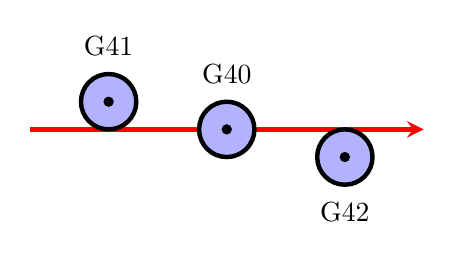
\begin{tikzpicture}[ultra thick]
\draw[->,red,>=stealth]  (0,0) -- (5,0);
\draw[fill=blue!30] (1,10pt) circle (10pt) circle (1pt);
\draw[fill=blue!30] (2.5,0) circle (10pt) circle (1pt);
\draw[fill=blue!30] (4,-10pt) circle (10pt) circle (1pt);
\node at (1,30pt) {G41};
\node at (2.5,20pt) {G40};
\node at (4,-30pt) {G42};
\end{tikzpicture}

\caption{刀补位置}
\label{fig:7-5}
\end{figure}

2、补偿值的设定:

通过参数进行设定:

[OfFset]---[补偿]----[位置号]----[D形状+D磨shen损]

3、指令的格式:

在开始刀补的位置,结合G1指令设定补偿方向及补偿值位置号,在结束的位置,用G40结合G1指令即可:

G41/G42 G1 X\_ Y\_  D\_;

……

G40 G1 X\_ Y\_;

4、补偿平面

可以在G18及G19平面上进行刀具半径补偿,(常用于球头刀)

5、补偿过程分析:

1)刀具半径补偿建立:当输入BS缓冲器的程序段包含有G41/G42命令时,系统认为此时已进入刀补建立状态。当以下条件成立时,加工中心以移动坐标轴的形式开始补偿动作。 

a. 有G41或G42被指定; 

b. 在补偿平面内有轴的移动; 

c. 指定了一个补偿号或已经指定一个补偿号但不能是D00;
 
d. 偏置(补偿)平面被指定或已经被指定; 

e. G00或G01模式有效。 

2) 补偿模式:在刀具补偿进行期间,刀具中心轨迹始终偏离编程轨迹一个刀具半径值的距离。此时半径补偿在G00、G01、G02、G03情况下均有效。 

3) 取消补偿:使用G40指令消去程序段偏置值,使刀具撤离工件,回到起始位置,从而使刀具中心与偏程轨迹重合。当以下两种情况之一发生时加工中心补偿模式被取消。

①给出G40同时要有补偿平面内坐标轴移动。

②刀具补偿号为D00。

4)不同平面内的半径补偿 

刀具半径补偿用G17、G18、G19命令在被选择的工作平面内进行补偿。即当G18命令执行后,刀具半径补偿仅影响X、Z移动,而对Y轴没有作用。


\subsubsection{注意事项}
1、G41/G42必须与G1/G0结合使用,不可在G2/G3圆弧指令下使用。

2、刀具必须在加工平面内有移动。

3、使用与取消必须成对使用。

4、加工前必须设定其补偿值。

5、切入前指定、切出后取消。


\subsubsection{编程实例}
1、在数控铣床或加工中心上加工如图\ref{fig:7-2}所示的零件,试完成程序的编写。
\begin{figure}[h]
	\centering
	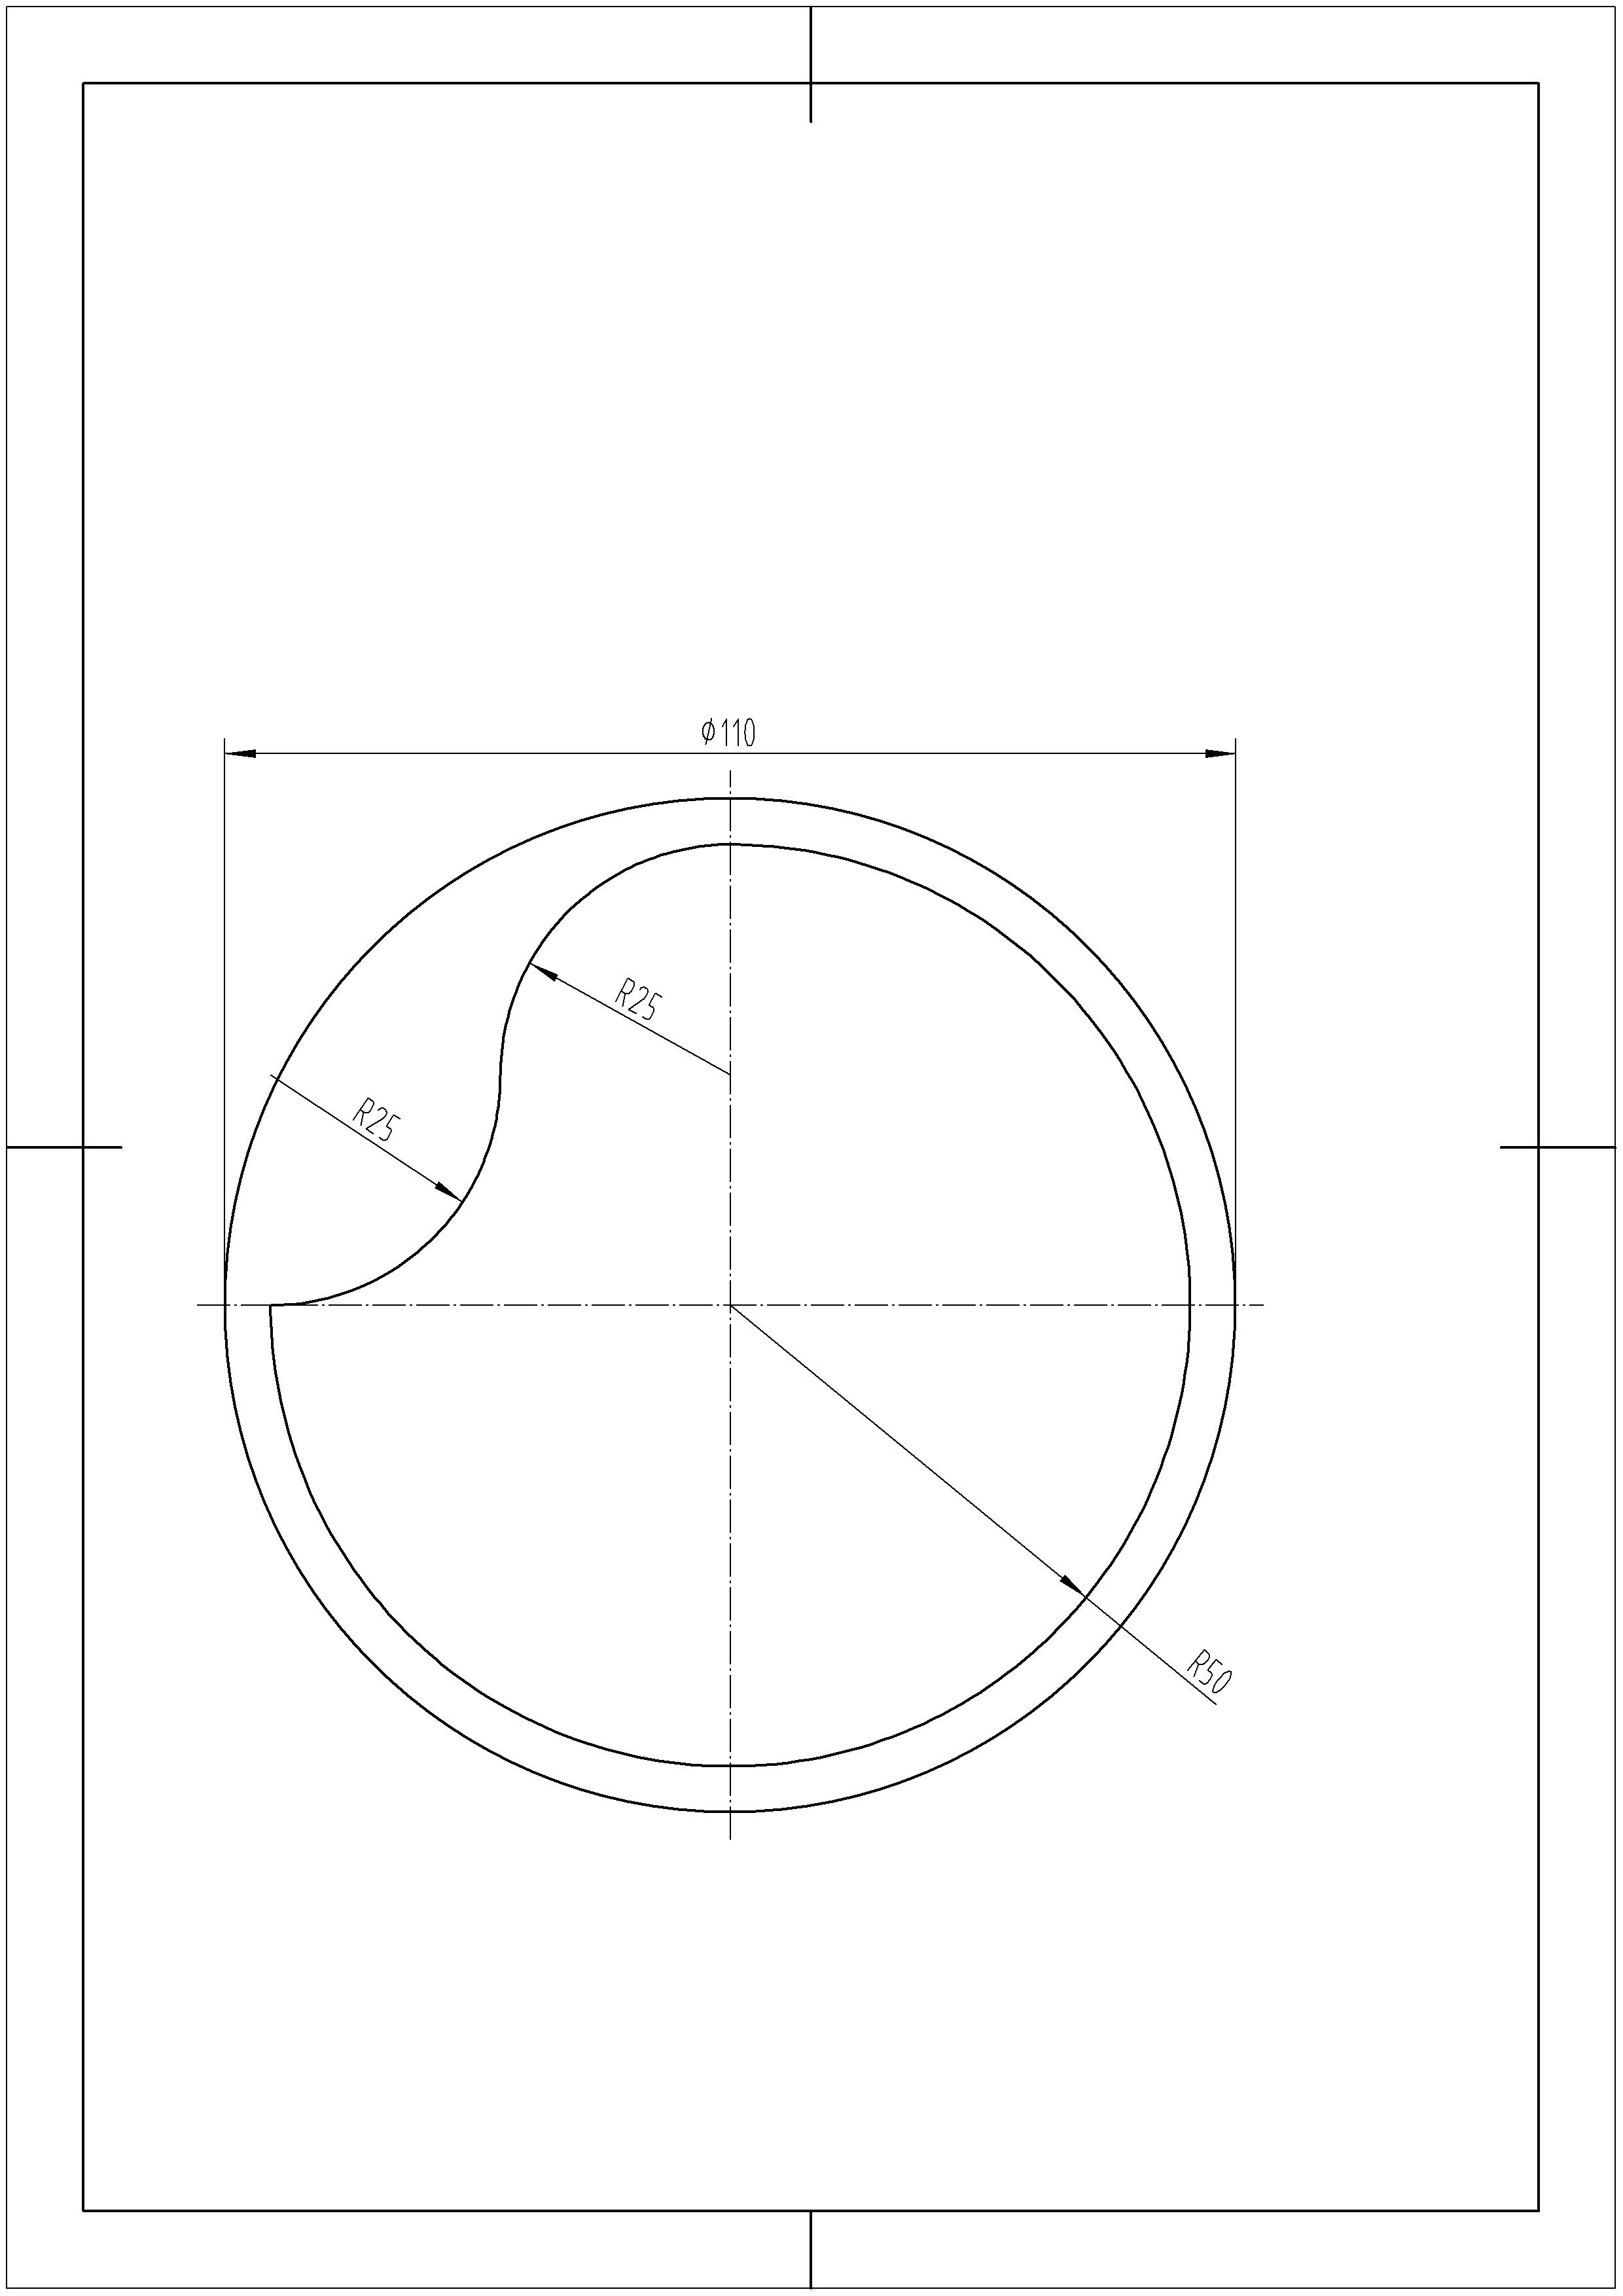
\includegraphics[width=0.8\linewidth,trim=40 150 70 220,clip]{data/image/7-1.jpg}
	\caption{刀补实例1}
	\label{fig:7-2}
\end{figure}

2、在数控铣床或加工中心上加工如图\ref{fig:7-3}所示的零件,试完成程序的编写。

\begin{figure}[h]
	\centering
	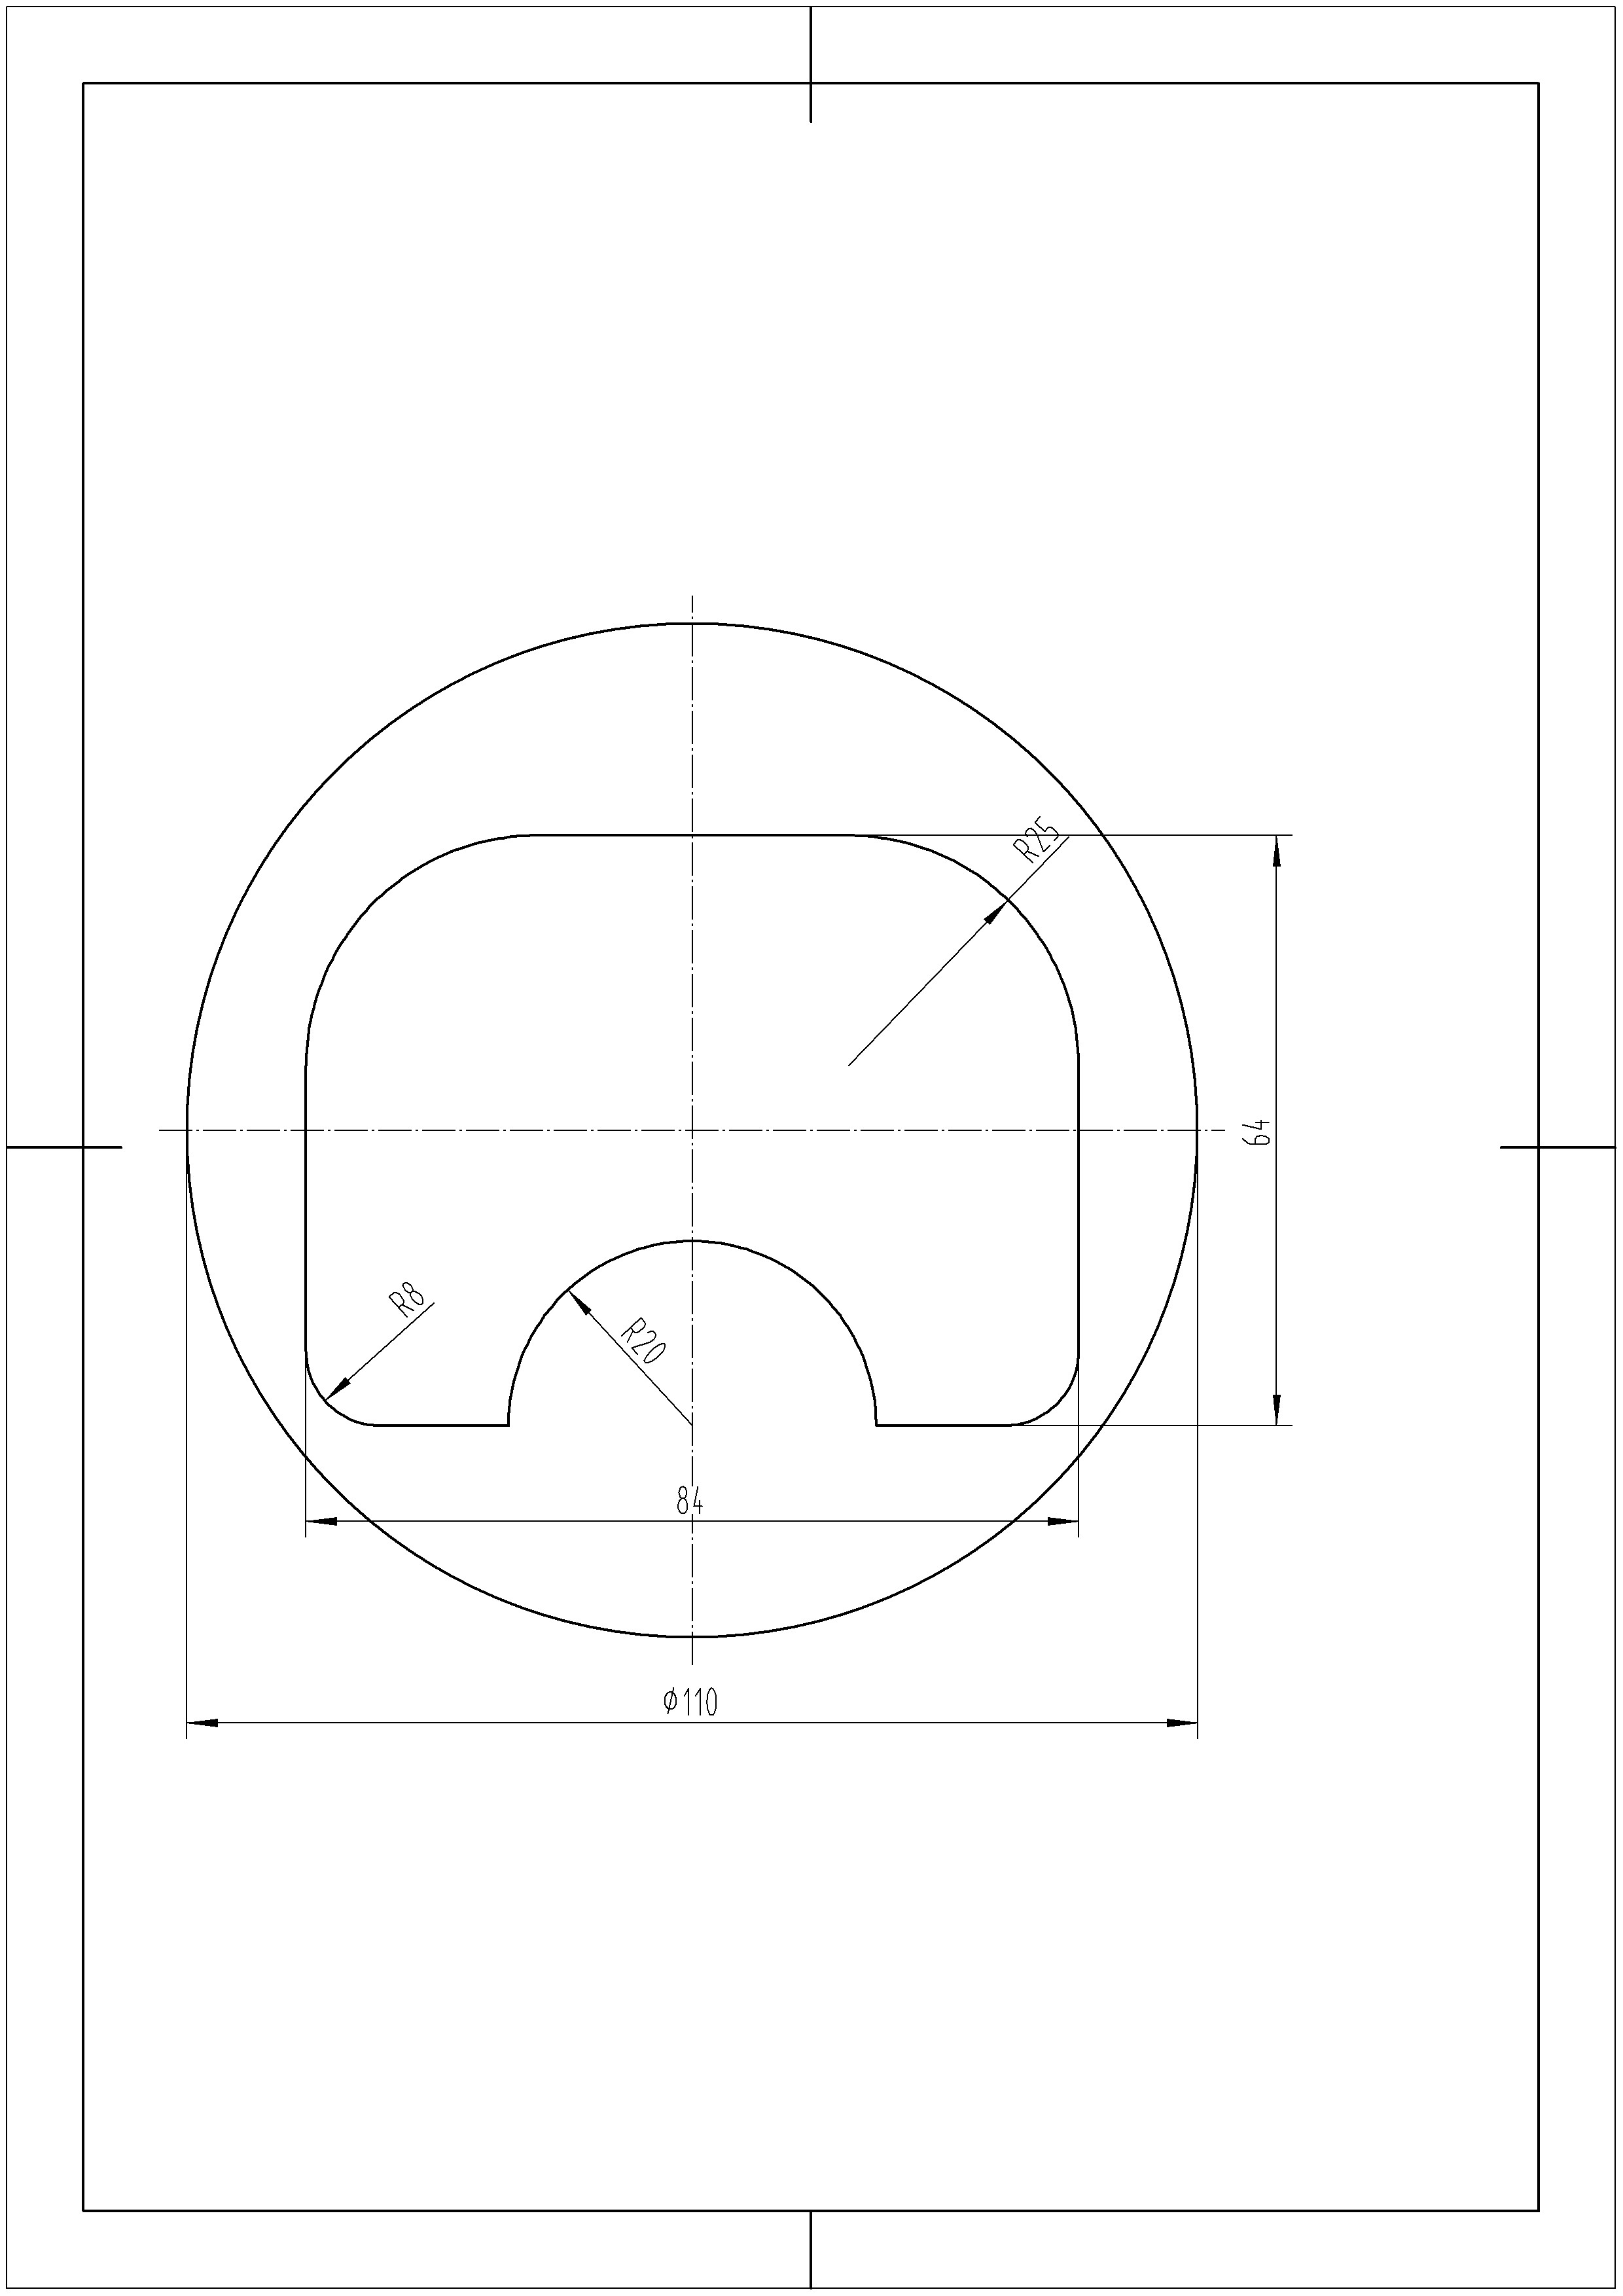
\includegraphics[width=0.8\linewidth,trim=40 150 70 220,clip]{data/image/7-2.jpg}
	\caption{刀补实例2}
	\label{fig:7-3}
\end{figure}


\subsection{课堂小结}
\begin{enumerate}[1、]
\item 刀补的概念
\item G40、G41/G42指令的使用;
\item 注意事项;
\item 刀补的编程;
\end{enumerate}

\vfill
\subsection{布置作业}
\begin{enumerate}[1、]
	\item 写出上面的程序。
	\item 习题集。
\end{enumerate}
\vfill
\jxhj{%教学后记
	}
\skrq{%授课日期
	2017年10月10日 4-5节}
\ktmq{%课题名称
	 刀具半径补偿的应用(一)}
\jxmb{%教学目标,每行前面要加 \item
	\item 掌握用刀补进行精加工;
	\item 掌握刀补值的计算;
	\item 会用G41/G42刀具半径指令编写程序;
	\item 了解常用切入切出的方法。
 }
\jxzd{%教学重点,每行前面要加 \item
	\item 用刀补进行精加工;
	\item 刀补值的计算。 }
\jxnd{%教学难点,每行前面要加 \item
	\item 刀补值的计算。 }
\jjff{%教学方法
	通过讲述、举例、演示、分析法来说明;}

\makeshouye %制作教案首页

%%%%教学内容
\subsection{组织教学}
\begin{enumerate}[\hspace{2em}1、]
	\item 集中学生注意力;
	\item 清查学生人数;
	\item 维持课堂纪律;
\end{enumerate}
\subsection{复习导入及主要内容}
\begin{enumerate}[1、]
\item 刀补的概念
\item G40、G41/G42指令的使用;
\item 注意事项;
\item 刀补的编程;
\item 在数控铣床或加工中心上加工如图\ref{fig:8-1}所示的零件,试完成程序的编写。(试用I、J、K编写,凸台高5mm)

\begin{figure}[h]
	\centering
	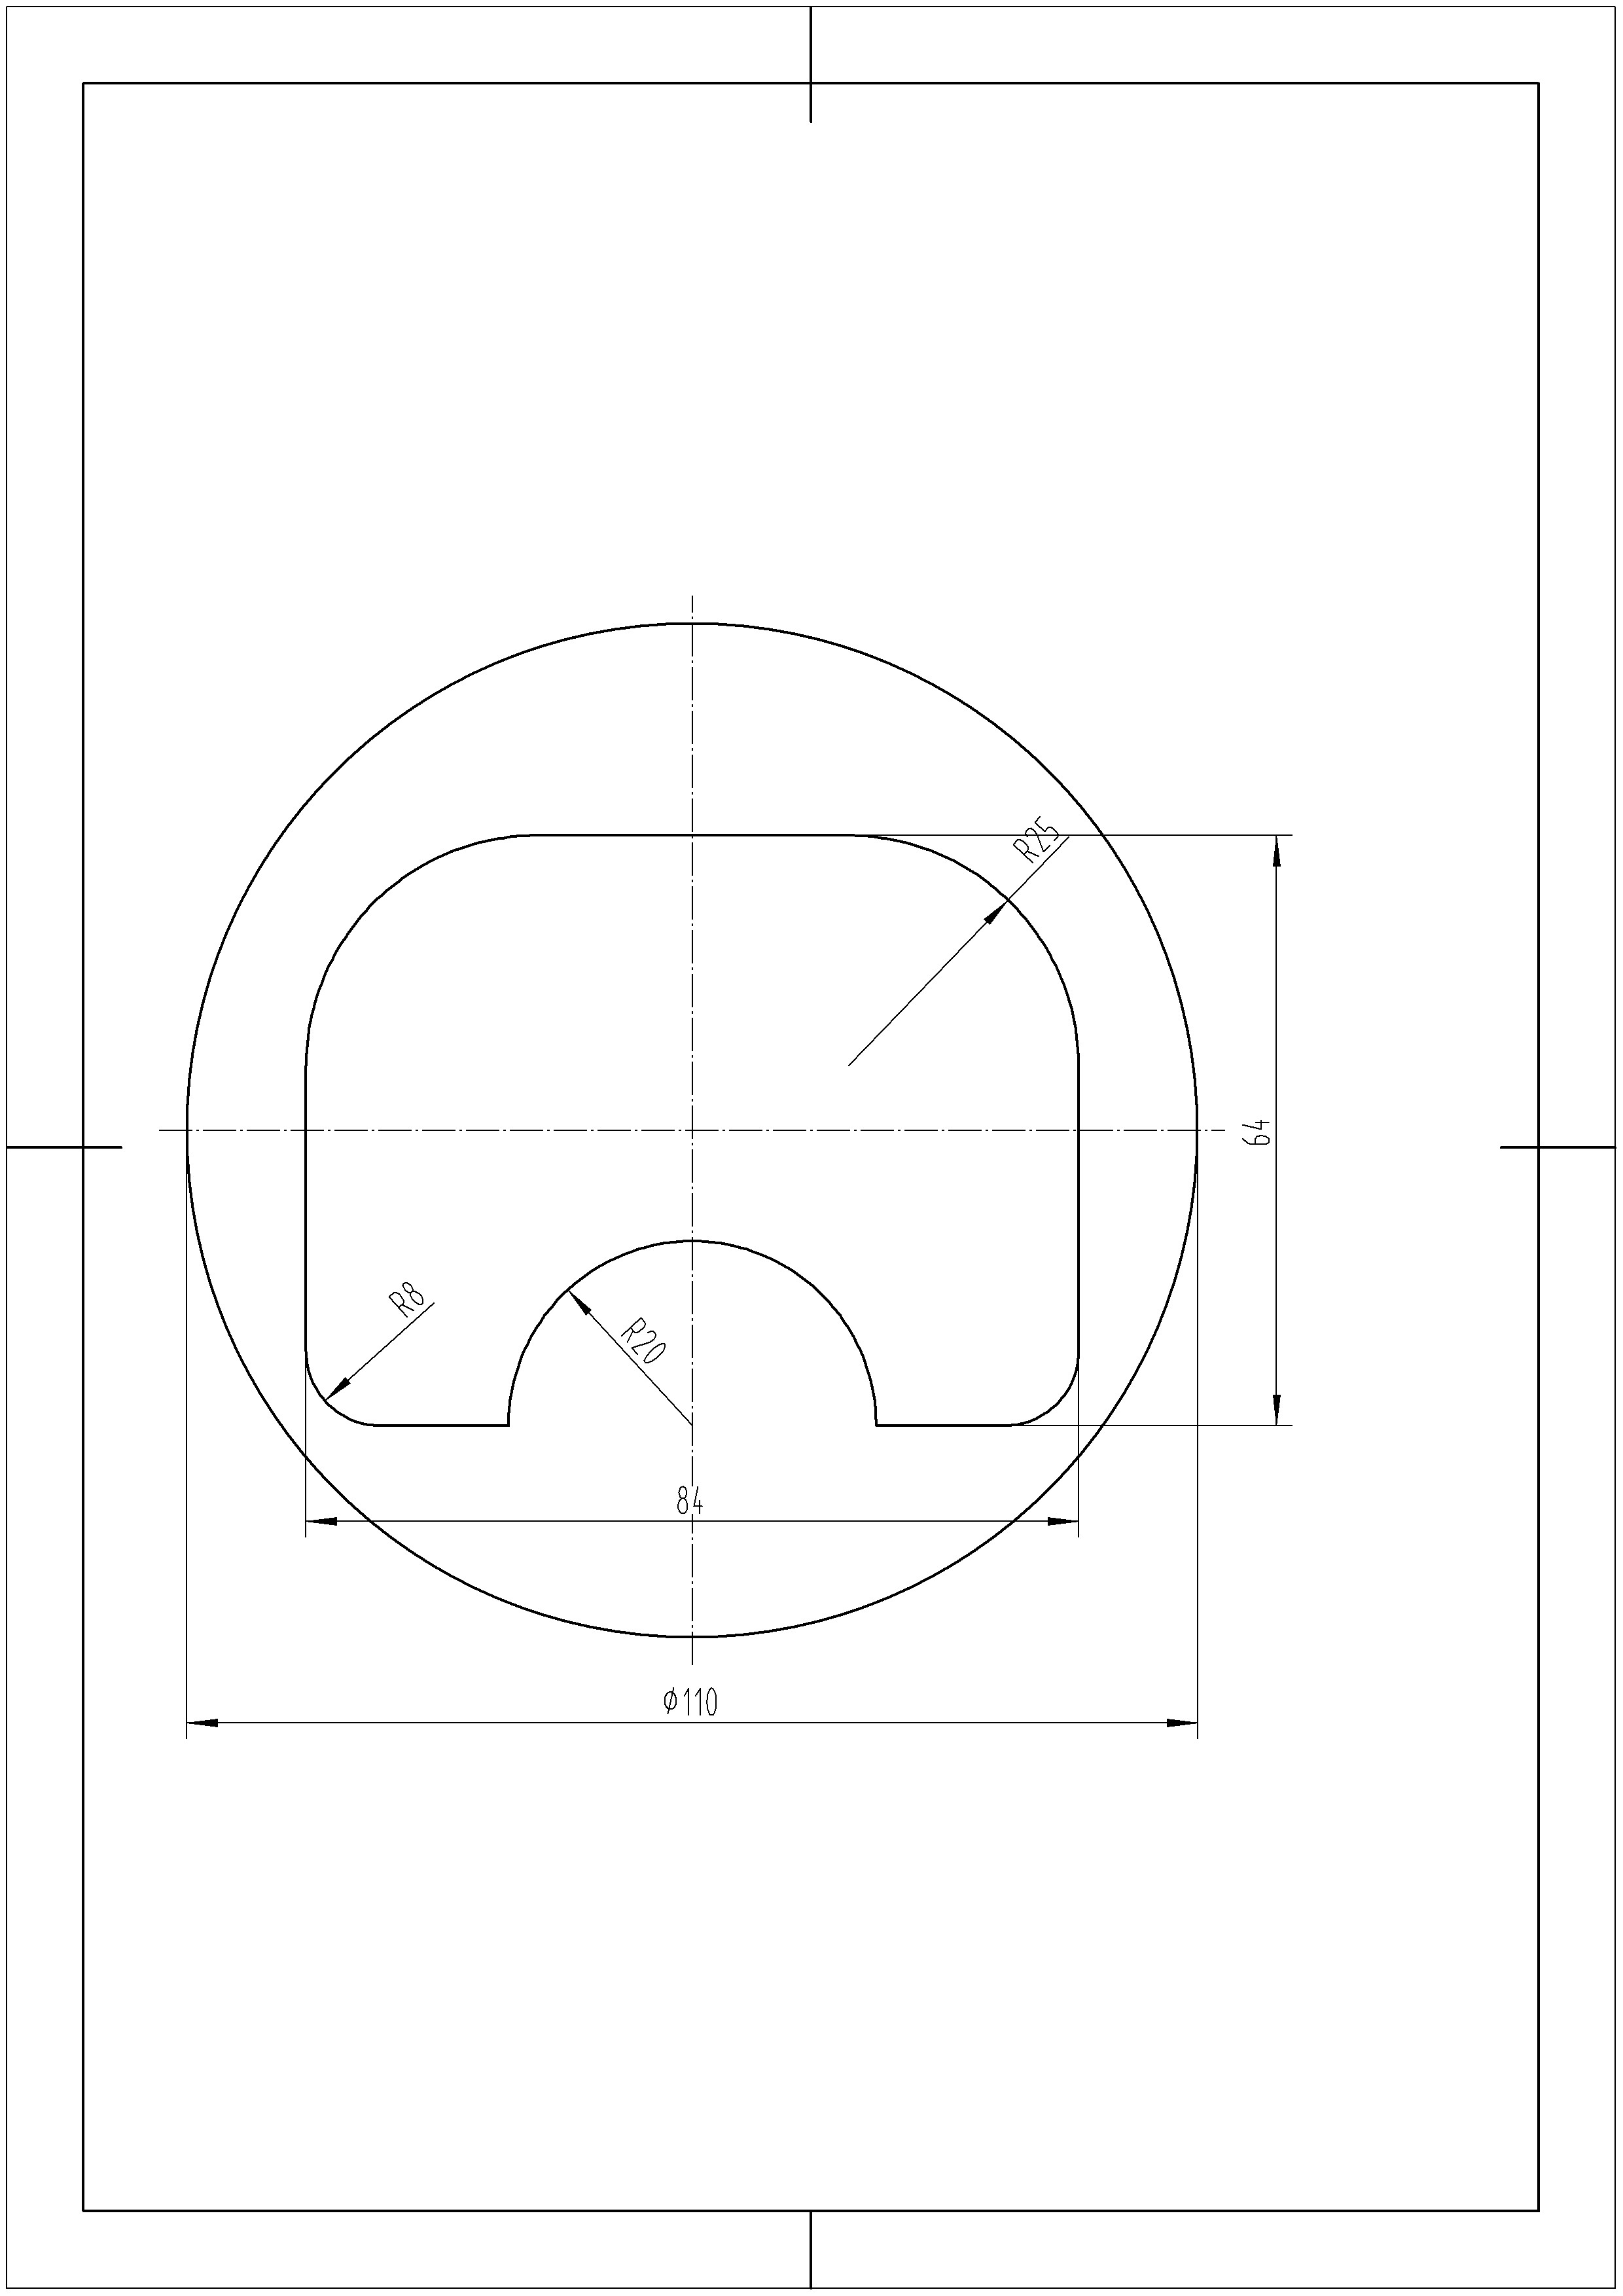
\includegraphics[width=0.8\linewidth,trim=40 150 70 220,clip]{data/image/7-2.jpg}
	\caption{复习实例2}
	\label{fig:8-1}
\end{figure}
\end{enumerate}


\subsection{教学内容及过程}

\subsubsection{刀具半径补偿}

由CNC系统内部使刀具在加工时,自动偏移一个刀具半径。
简化编程的难度。

指令G40、G41/G42

1、补偿方向的确定:

ISO 标准规定,当刀具中心轨迹在编程轨迹前进方向的左边时,称为左刀补,用G41表示;刀具中心轨迹在编程轨迹前进方向的右边时,称为右刀补,用G42表示;注销刀具半径补偿时用G40表示。

\begin{figure}[h]
	\centering
	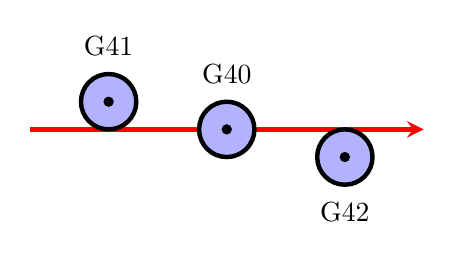
\begin{tikzpicture}[ultra thick]
	\draw[->,red,>=stealth]  (0,0) -- (5,0);
	\draw[fill=blue!30] (1,10pt) circle (10pt) circle (1pt);
	\draw[fill=blue!30] (2.5,0) circle (10pt) circle (1pt);
	\draw[fill=blue!30] (4,-10pt) circle (10pt) circle (1pt);
	\node at (1,30pt) {G41};
	\node at (2.5,20pt) {G40};
	\node at (4,-30pt) {G42};
	\end{tikzpicture}
	\caption{刀补位置}
	\label{fig:8-1}
\end{figure}

2、补偿值的设定:

通过参数进行设定:

[OfFset]---[补偿]----[位置号]----[D形状+D磨shen损]

3、指令的格式:

在开始刀补的位置,结合G1指令设定补偿方向及补偿值位置号,在结束的位置,用G40结合G1指令即可:

G41/G42 G1 X\_ Y\_  D\_;

……

G40 G1 X\_ Y\_;

4、补偿平面

可以在G18及G19平面上进行刀具半径补偿,(常用于球头刀)

5、补偿过程分析:

1)刀具半径补偿建立:当输入BS缓冲器的程序段包含有G41/G42命令时,系统认为此时已进入刀补建立状态。当以下条件成立时,加工中心以移动坐标轴的形式开始补偿动作。 

a. 有G41或G42被指定; 

b. 在补偿平面内有轴的移动; 

c. 指定了一个补偿号或已经指定一个补偿号但不能是D00;

d. 偏置(补偿)平面被指定或已经被指定; 

e. G00或G01模式有效。 

2) 补偿模式:在刀具补偿进行期间,刀具中心轨迹始终偏离编程轨迹一个刀具半径值的距离。此时半径补偿在G00、G01、G02、G03情况下均有效。 

3) 取消补偿:使用G40指令消去程序段偏置值,使刀具撤离工件,回到起始位置,从而使刀具中心与偏程轨迹重合。当以下两种情况之一发生时加工中心补偿模式被取消。

①给出G40同时要有补偿平面内坐标轴移动。

②刀具补偿号为D00。

4)不同平面内的半径补偿 

刀具半径补偿用G17、G18、G19命令在被选择的工作平面内进行补偿。即当G18命令执行后,刀具半径补偿仅影响X、Z移动,而对Y轴没有作用。


\subsubsection{注意事项}
1、G41/G42必须与G1/G0结合使用,不可在G2/G3圆弧指令下使用。

2、刀具必须在加工平面内有移动。

3、使用与取消必须成对使用。

4、加工前必须设定其补偿值。

5、切入前指定、切出后取消。

\subsubsection{加工实例}
毛坯:φ110*35

刀具:φ12立铣刀

加工路径:如图\ref{fig:8-2}所示:

\begin{figure}[h]
	\centering
	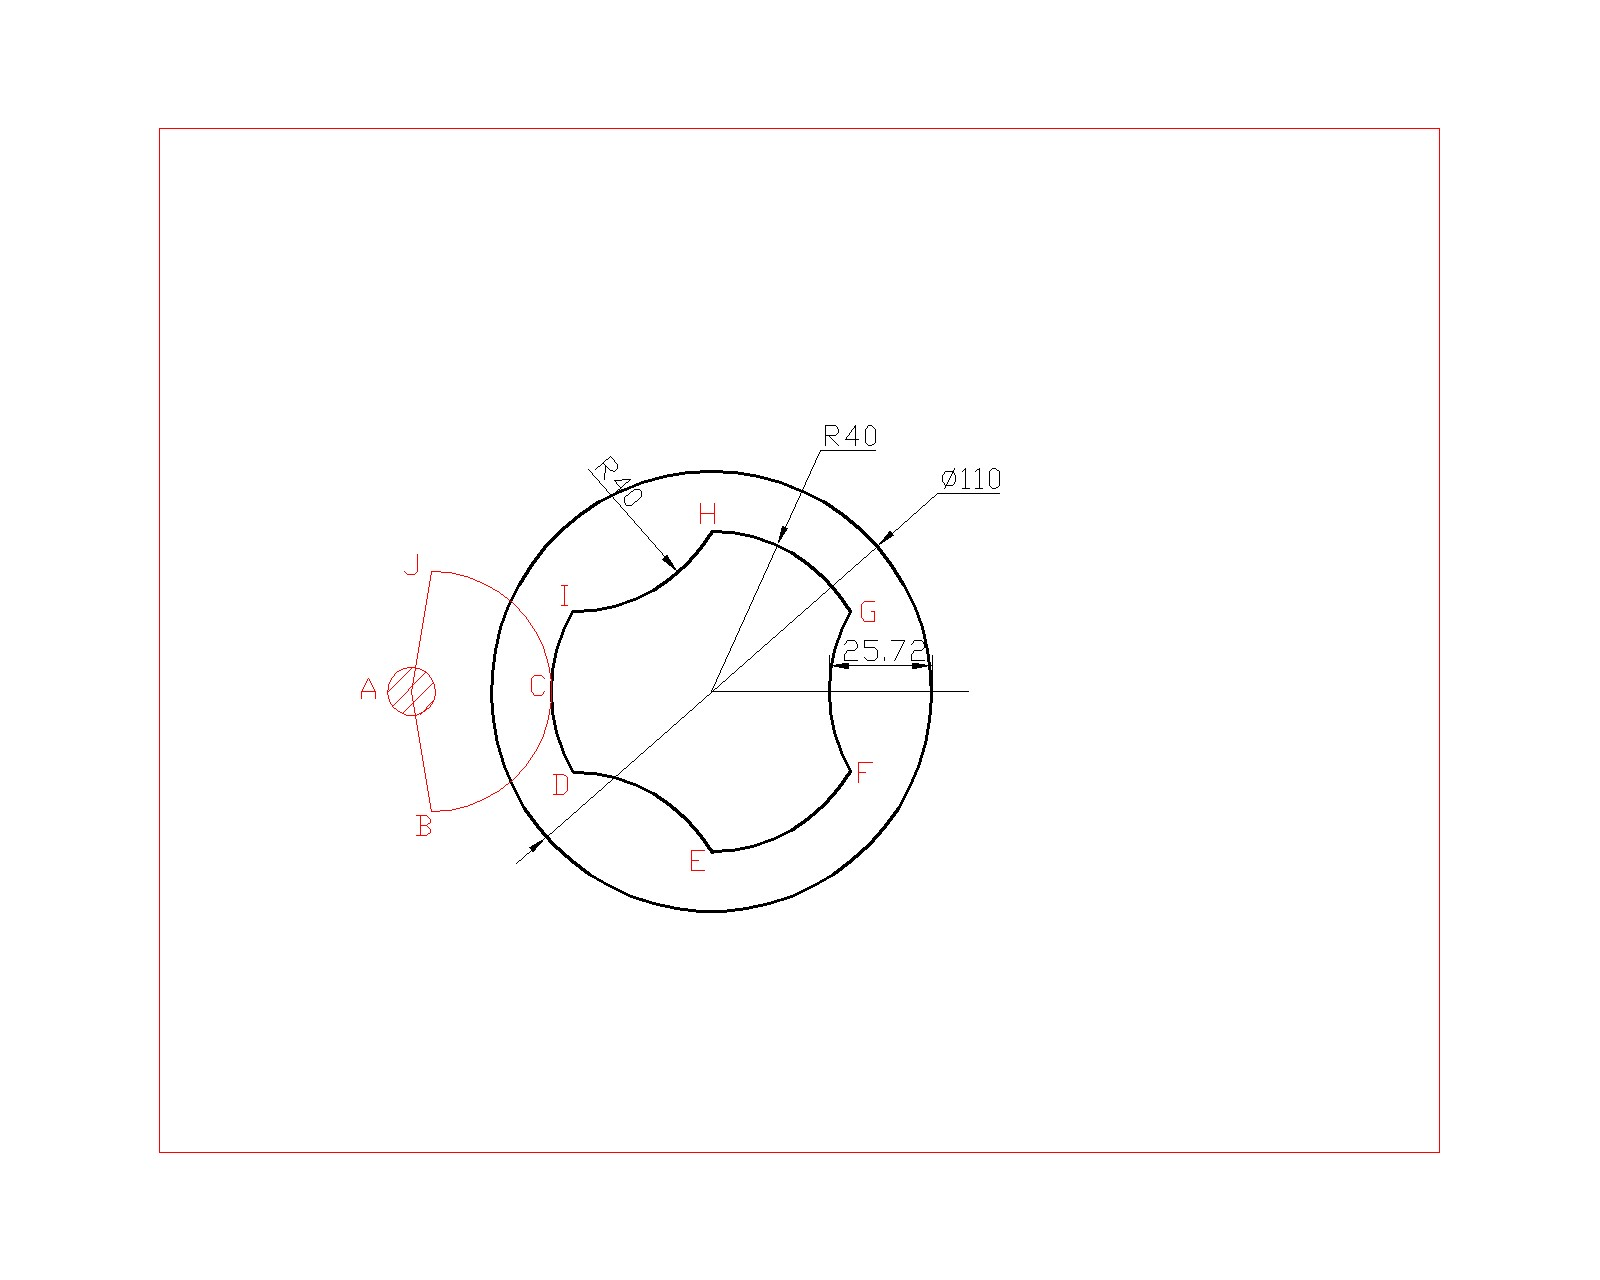
\includegraphics[width=0.8\linewidth,trim=280 250 430 280,clip]{data/image/8-2.jpg}
	\caption{刀补实例}
	\label{fig:8-2}
\end{figure}

参考程序:
\begin{lstlisting}
G54G17G40G49G90
M03 S300
G0 X-70.0 Y0
Z5.0
G01 Z-5.0 F500
G41 G01 X-60 Y-20 D01
G03 X-40.0 Y0 R20.0
G02 X-34.641 Y20.0 R40.0
G03 X0 Y40.0 R40.0
G02 X34.641 Y20 R40.0
G03 Y-20.0 R40.0
G02 X0 Y-40.0 R40.0
G03 X-34.641 Y-20 R40.0
G02 X-40 Y0 R40.0
G03 X-60 Y0 R20.0
G40 G01 X-70 Y0
G0 Z30
M05
M30
\end{lstlisting}

\subsubsection{刀具半径补偿值的确定}

1、粗加工:

为半精/精加留余量:0.2-0.6 (单边)

Offset=D/2+余量

2、半精加工:

为精加留余量:0.1-0.2 (单边)

Offset=D/2+余量

3、精加工:

Offset= Offset (上次)+修正

修正=(理论值-测量值)双边/2 

4、处多余材料:

Offset值不能太大



\subsection{课堂小结}
\begin{enumerate}[1、]
\item 刀补的概念
\item G40、G41/G42指令的使用;
\item 注意事项;
\item 刀补的编程;
\item 刀补值的计算。
\end{enumerate}

\vfill
\subsection{布置作业}
\begin{enumerate}[1、]
	\item 写出上面的程序。
\item 习题集。
\end{enumerate}
\vfill
\jxhj{%教学后记
	}
\skrq{%授课日期
	2017年10月12日 4-5节}
\ktmq{%课题名称
	 刀具半径补偿的应用(二)}
\jxmb{%教学目标,每行前面要加 \item
	\item 掌握用刀补去残料。
	\item 掌握去材料刀补的计算;
	\item 掌握多个刀补的编程;
	\item 巩固粗/精加工刀补值的确定。
 }
\jxzd{%教学重点,每行前面要加 \item
	\item 用刀补去残料;
	\item 去材料刀补的计算。 }
\jxnd{%教学难点,每行前面要加 \item
	\item 去材料刀补的计算。 }
\jjff{%教学方法
	通过讲述、举例、演示法来说明;}

\makeshouye %制作教案首页

%%%%教学内容
\subsection{组织教学}
\begin{enumerate}[\hspace{2em}1、]
	\item 集中学生注意力;
	\item 清查学生人数;
	\item 维持课堂纪律;
\end{enumerate}
\subsection{复习导入及主要内容}
\begin{enumerate}[1、]
\item 刀补的概念
\item G40、G41/G42指令的使用;
\item 注意事项;
\item 刀补的编程;
\item 刀补值的计算。
\end{enumerate}



\subsection{教学内容及过程}

\subsubsection{去残料刀补的计算}
步骤

1、计算最大残料值

以实际毛坯尺寸来计算

2、根据刀具直径确定粗加工刀补值

刀具半径+单边余量(0.2-0.6)

3、根据刀具直径确定加工宽度

刀具直径的50\%-80\%

也可: (残料-粗加工刀补)/次数

4、刀补值的计算:

去残料刀补=粗加工刀补+加工宽度×次数

5、判断残料是否去完

最大刀补+刀具半径>最大残料  表示已去完

6、其他:

根据最大刀补确定切入切出半径

最大刀补不能大于最小内凹圆弧半径

\subsubsection{去残料刀补的计算}

\begin{figure}[h]
	\centering
	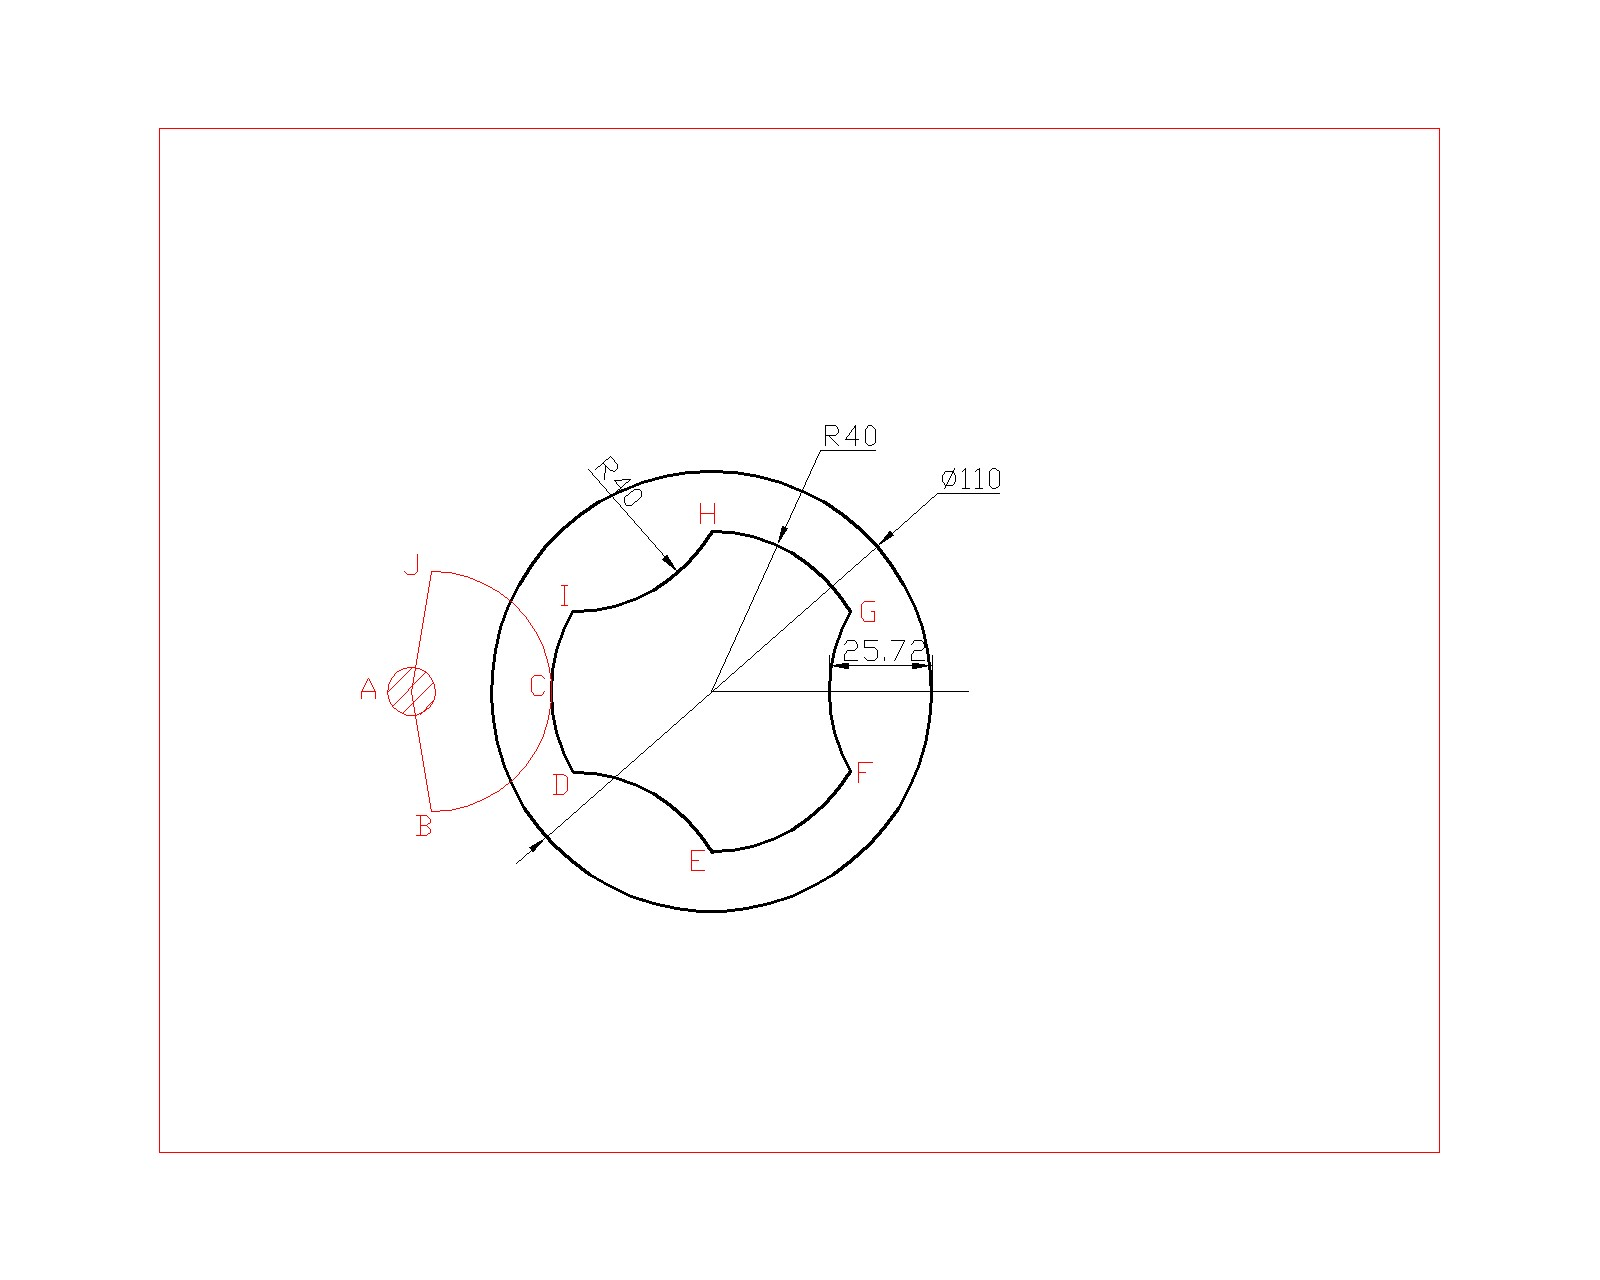
\includegraphics[width=0.8\linewidth,trim=280 250 430 280,clip]{data/image/8-2.jpg}
	\caption{刀补实例}
	\label{fig:9-1}
\end{figure}

1、计算最大残料值

以实际毛坯尺寸来计算  25.72

2、根据刀具直径确定粗加工刀补值

刀具半径+单边余量(0.2-0.6)

直径为12的立铣刀   6.5

3、根据刀具直径确定加工宽度

刀具直径的50\%-80\%   取10.

也可: (残料-粗加工刀补)/次数

4、刀补值的计算:

去残料刀补=粗加工刀补+加工宽度×次数

D2 16.5

D1 26.5

5、判断残料是否去完

最大刀补+刀具半径>最大残料  表示已去完

6、切入切出半径:

取R30

7、参考程序:
\begin{lstlisting}
O0001 (粗加工)
G54G17G40G49G90
M3S500
G1Z30.0F2000
X-75.0Y0
Z5.0
Z-5.0F200
G41X-70.Y-30.D1    (D1=26.5)
G3X-40.Y0R30.
G2X-34.64Y20.R40.
G3X0Y40.R40.
G2X34.64Y20.R40.
G3Y-20.R40.
G2X0Y-40.R40.
G3X-34.64Y-20.R40.
G2X-40.Y0R40.
G3X-70.Y30.R30.
G40G1X-75.Y0
G41X-70.Y-30.D1      (D2=16.5)
G3X-40.Y0R30.
G2X-34.64Y20.R40.
G3X0Y40.R40.
G2X34.64Y20.R40.
G3Y-20.R40.
G2X0Y-40.R40.
G3X-34.64Y-20.R40.
G2X-40.Y0R40.
G3X-70.Y30.R30.
G40G1X-75.Y0
G41X-70.Y-30.D1      (D3=6.5)
G3X-40.Y0R30.
G2X-34.64Y20.R40.
G3X0Y40.R40.
G2X34.64Y20.R40.
G3Y-20.R40.
G2X0Y-40.R40.
G3X-34.64Y-20.R40.
G2X-40.Y0R40.
G3X-70.Y30.R30.
G40G1X-75.Y0
M5
M30
\end{lstlisting}
精加工程序另写

\subsection{课堂小结}
\begin{enumerate}[1、]
	\item 去残料刀补的计算;
	\item 程序的编写
	
\end{enumerate}

\vfill
\subsection{布置作业}
\begin{enumerate}[1、]
	\item 写出上面的程序。
\item 习题集。 
\end{enumerate}
\vfill
\jxhj{%教学后记
	}
\skrq{%授课日期
	2017年10月17日 4-5节}
\ktmq{%课题名称
	 子程序概述及Z向分层}
\jxmb{%教学目标,每行前面要加 \item
	\item 掌握子程序的概念;
	\item 掌握子程序命令的使用;
	\item 掌握使用子程序进行Z向分层的思路;
	\item 掌握掌握子程序的编程。 }
\jxzd{%教学重点,每行前面要加 \item
	\item Z向分层的思路;
	\item 子程序命令的使用。 }
\jxnd{%教学难点,每行前面要加 \item
	\item Z向分层的思路。 }
\jjff{%教学方法
	通过讲述、举例、演示法来说明;}

\makeshouye %制作教案首页

%%%%教学内容
\subsection{组织教学}
\begin{enumerate}[\hspace{2em}1、]
	\item 集中学生注意力;
	\item 清查学生人数;
	\item 维持课堂纪律;
\end{enumerate}
\subsection{复习导入及主要内容}
\begin{enumerate}[1、]
	\item 用刀补去残料的思路。
\item 去材料刀补的计算;
\item 多个刀补的编程;
\item 巩固粗/精加工刀补值的确定。
\end{enumerate}

\subsection{教学内容及过程}

\subsubsection{Fanuc上子程序的格式及调用}
[ 格式 ]
■子程序构成

O55; 子程序名

G1 ...

.

.

.

M99;子程序结束


■	子程序呼叫

M98P55L1

[ 说明 ]

当主程序呼叫子程序时,它是一重子程序呼叫。因此,子程序可以做四重呼叫,。                                                 

一个单个呼叫指令可以重复呼叫子程序最多到9999次。

对于兼容的编程装置,在第一个单节里,Nxxxx可以代替子程序O(或:)跟着的数字。在N后面的顺序号被认为是子程序号。

[ 注意 ]
1.	M98和M99信号不输出到机床。
2.	不到位址指定的子程序号,输出报警(No. 078)。

[ 举例 ]

☆M98 P51002;

这条指令指定“呼叫子程序(程序号1002)5次”。

子程序呼叫指令(M98P\_\_\_)可以在移动指令单节中指定。

☆X1000.0 M98 P1200;

这个例子在X轴移动之后呼叫子程序(子程序号 1200)。

☆从主程序呼叫子程序的执行顺序

主程序                   子程序

N0010 O;               N0010 O;   
      
N0020 O;               N0020 O;    
     
N0030 M98 P21010;      N0030 M98 P21010; 
                
N0040 O;               N0040 O;
             
N0050 O;               N0050 O;

子程序可以象主程序呼叫子程序一样呼叫另一个子程序。

[ 特殊用途 ]
 
■主程序中使用M99

如果在主程序中执行M99,控制返回主程序开头。

举例说,/M99放在程序中并执行M99;

在主程序的适当位置设定选择性单节跳跃功能,在执行主程序时关掉。

当执行M99时,控制返回到主程序的开头,然后主程序从头开始重复执行。

当选择性单节跳跃功能设定关时,重复执行程序。当选择性单节跳跃功能设定开时,/M99单节被跳过;控制进入下一个单节继续执行。

二、使用子程序的场合:

1、同一零件上有重复加工的部位

2、批量加工,一次加工多个相同的工件

3、同一个零件上有多个不同形状的加工轮廓

可使程序看起来方便,简单

不使用的场合:

自动编程不用子程序:


1、多程序传输不方便

2、自动编程子程序完成后,修改的内容多,

三、编程实例

方形:

\begin{lstlisting}
O0001
G54G17G40G49G90
M3S500
G1Z30.F2000
X-50.Y0
Z5.0
Z0F200
D1M98P40002
G1Z30.F2000
M4
M30
O0002
G91G1Z-5.0
G90G41X-40.Y0
G3X-30.Y0R10.
G1Y30.
….
M99
\end{lstlisting}

\subsection{课堂小结}
\begin{enumerate}[1、]
	\item 子程序的概念;
	\item 子程序的组成;
	\item 子程序的调用;
	\item 子程序的使用。
\end{enumerate}

\vfill
\subsection{布置作业}
\begin{enumerate}[1、]
	\item 运用子程序编写一个程序。 
\end{enumerate}
\vfill
\jxhj{%教学后记
	}
\skrq{%授课日期
	2017年10月19日 4-5节}
\ktmq{%课题名称
	 子程序的XY向分层}
\jxmb{%教学目标,每行前面要加 \item
	\item 掌握子程序指令的使用;
	\item 掌握用子程序编程;
	\item 掌握用子程序及刀补实现XY向分层;
	\item 掌握子程序的嵌套调用。 }	
\jxzd{%教学重点,每行前面要加 \item
	\item 用子程序及刀补实现XY向分层;
	\item 子程序的嵌套调用。 }
\jxnd{%教学难点,每行前面要加 \item
	\item 用子程序及刀补实现XY向分层。 }
\jjff{%教学方法
	通过讲述、举例、演示法来说明;}

\makeshouye %制作教案首页

%%%%教学内容
\subsection{组织教学}
\begin{enumerate}[\hspace{2em}1、]
	\item 集中学生注意力;
	\item 清查学生人数;
	\item 维持课堂纪律;
\end{enumerate}
\subsection{复习导入及主要内容}
\begin{enumerate}[1、]
	\item 子程序的概念;
\item 子程序的组成;
\item 子程序的调用;
\item 子程序的使用。
\end{enumerate}


\subsection{教学内容及过程}

\subsubsection{加工实例分析}

如图\ref{fig:11-1}所示:加工凸台零件,高12mm。

\begin{figure}[h]
	\centering
	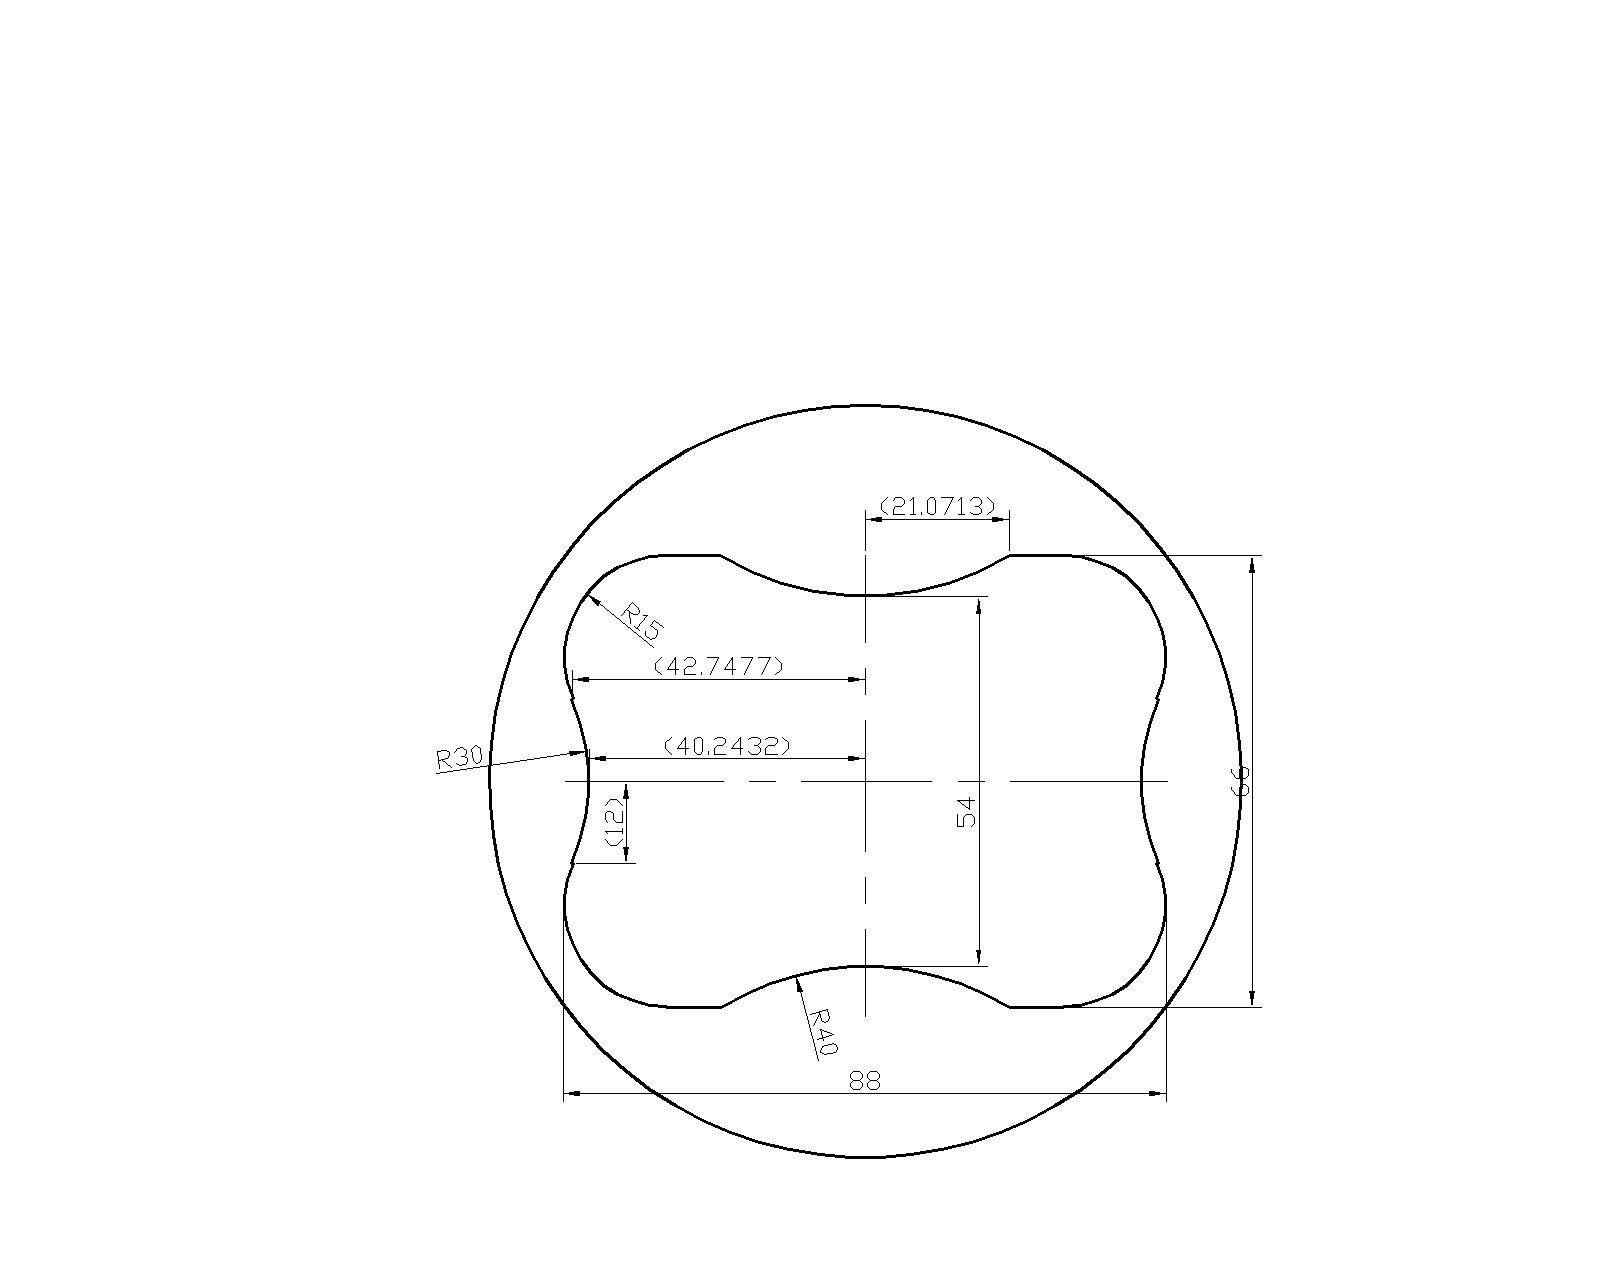
\includegraphics[width=0.7\linewidth,trim=250 50 150  250,clip]{data/image/11-1.jpg}
	\caption{刀补实例}
	\label{fig:11-1}
\end{figure}

毛坯:\diameter 110*35

刀具:\diameter 12立铣刀

1、Z向分层加工:

高12mm     3mm*4次     深度等分下刀

用G91 G01 Z-3.0 F300; Z方向要先定好位

是Z方向

2、XY向分层,平面上的等分铣削:

方法:用不同的刀具半径值:

A、刀具补偿值的确定:(由小到大确定)

大=较大+B

较大=小+B

小=D/2+(0.2-0.6)

B=50-80\% *D 

判断是否把多余材料去完

B、切入/切出圆弧半径:

R>最大的刀补值

C、XY平面内的定位

第一次铣削后,刀具位置应回到原来位置

3、参考程序:

主程序:


\begin{lstlisting}
O0001
G54 G17 G40 G49 G90
M03 S300
G01 X0 Y75.0 F800
Z0
M98 P40002
G01 Z30.0
M05
M30
\end{lstlisting}

下刀子程序
\begin{lstlisting}
O0002
G91 G01 Z-3.0 
G90
D1 M98 P3
D2 M98 P3
D3 M98 P4
M99
\end{lstlisting}
轮廓子程序
\begin{lstlisting}
O0003
G41 G01 X-40.0 Y67.0
G03 X21.071 Y33.0 R40.0
G1 X39
G03 X42.748 Y12.0 R15.0
G02 Y-12.0 R30.0
G03 X39 Y-33.0 R15.0
G01 X21.071
G03 X-21.071 R40.0
G01 X-39.0
G03 X-42.748 Y-12.0 R15.0
G02 Y12.0 R30.0
G03 X-39.0 Y33.0 R15.0
G01 X-21.071 
G03 X40.0 Y67.0 R40.0
G40 G01 X0 Y75.0
M99
\end{lstlisting}

\subsubsection{使用子程序的场合}
1、同一零件上有重复加工的部位

2、批量加工,一次加工多个相同的工件

3、同一个零件上有多个不同形状的加工轮廓

可使程序看起来方便,简单

不使用的场合:

自动编程不用子程序:

1、多程序传输不方便

2、自动编程子程序完成后,修改的内容多。

\subsection{课堂小结}
\begin{enumerate}[1、]
	\item 子程序Z向分层;
	\item 子程序XY向分层;
	\item 子程序的应用。	
\end{enumerate}

\vfill
\subsection{布置作业}
\begin{enumerate}[1、]
	\item 用子程序编写一个Z向分层+XY向分层的程序。 
\end{enumerate}
\vfill
\jxhj{%教学后记
	}
\skrq{%授课日期
	2017年10月24日 4-5节}
\ktmq{%课题名称
	 siemens编程应用}
\jxmb{%教学目标,每行前面要加 \item
	\item 掌握Siemens上子程序指令的使用;
	\item 掌握Siemens上的编程;
	\item 掌握Siemens上的半径补偿;
	\item 掌握相关注意事项。 }
\jxzd{%教学重点,每行前面要加 \item
	\item Siemens上的编程;
	\item Siemens上的半径补偿。 }
\jxnd{%教学难点,每行前面要加 \item
	\item Siemens上的半径补偿。 }
\jjff{%教学方法
	通过讲述、举例、演示法来说明;}

\makeshouye %制作教案首页

%%%%教学内容
\subsection{组织教学}
\begin{enumerate}[\hspace{2em}1、]
	\item 集中学生注意力;
	\item 清查学生人数;
	\item 维持课堂纪律;
\end{enumerate}
\subsection{复习导入及主要内容}
\begin{enumerate}[1、]
\item 子程序Z向分层;
\item 子程序XY向分层;
\item 子程序的应用。
\end{enumerate}

\subsection{教学内容及过程}

\subsubsection{Siemens上的程序名}
Fanuc: O+四位数值 为程序号,

即1号和0001号为同一个程序。

0-7999: 用户使用。不能加密。

8000-8999: 机床生产商和用户使用,可加密。

9000-9999: 系统开发商使用,可加密。

主程号与子程序号不区分。

Siemens:  前两位为字母,后面任意。不能与系统已有的字
重名。

GX03  AAA  BBB   可以

GOTO10  CYCLE81   不可以

字程序:   L+四位数值组成

也可以与主程序使用一样的规格。

主程序的扩展名为  MPF

子程序的扩展名为  SPF

\subsubsection{Siemens上的G指令}
1、G1    G2/G3

Siemens  使用CR=\_\_表示半径。

Siemens上还有其他使用格式。

2、G4  暂停时间

Fanuc: G4 X\_\_/P—  X表示秒,P表示毫秒。

Sienem: G4 F\_\_   F表示秒。

3、G17  G18  G19

4、G20  G21    fanuc上 表示 英制 与公制

G70  G71   Siemens上 表示 英制 与公制

5、G27 G28 G29  Fanuc 表现 回参考点检查  回参考点  从参考点返回。

G74  回参考点

6、G40  G41  G42

补偿号   在Siemens上称为刀沿号

每一把刀具可以有9个切削刀沿。

7、G43 G44  G49  Fanuc 刀具长度补偿

T1D1  Siemens 上自动补偿。

8、G53 G54-G59

\subsubsection{Siemens上其他问题}

1、子程序结束 RET M17

2、子程序的调用 

子程序名  P\_\_ 调用次数

子程序的调用必须单独占用一个程序段。

\subsubsection{Siemens编程实例}
如图: 在数控机床上加工如图所示的零件,试用siemens
格式编程。

程序:
\begin{lstlisting}
GX01   粗加工
G54G17G40G90
T1D1
M3S500
G1Z30.F2000
X-55.Y0
Z5.
Z0F200
L1 P4
Z0
L2 P2
Z3.
Z30.F2000
M5
M2	
\end{lstlisting}

\begin{lstlisting}
L1   方形轮廓子程序
G91Z-2.5
G90
G41G1X-45.Y0
G3X-35.Y0CR=10.
G1Y35.
X35.
Y-35.
X-35.
Y0
G3X-45.Y10.CR=10.
G40G1X-55.Y0
M17
\end{lstlisting}

\begin{lstlisting}
L2  圆形轮廓子程序
G91G1Z-2.5
G90
G41G1X-40.Y-10.
G3X-30.Y0CH=10.
G2I30.
G3X-40.Y10.CH=10.
G40G1X-55Y0
RET
\end{lstlisting}

\begin{lstlisting}
GX01   精加工
G54G17G40G90
T2D1
M3S800
G1Z30.F2000
X-55.Y0
Z5.
Z-7.6F100  
L1 
Z-2.5
L2 
Z3.
Z30.F2000
M5
M2
\end{lstlisting}

\subsection{课堂小结}
\begin{enumerate}[1、]
	\item Siemens上的程序名;
	\item Siemens上的G指令;
	\item Siemen上的子程序;
	\item Siemens编程实例。
\end{enumerate}

\vfill
\subsection{布置作业}
\begin{enumerate}[1、]
	\item 用Siemens格式编程一个程序。
\end{enumerate}
\vfill
\jxhj{%教学后记
	}
\skrq{%授课日期
	2017年10月26日 4-5节}
\ktmq{%课题名称
	 平面及斜面加工工艺}
\jxmb{%教学目标,每行前面要加 \item
	\item 掌握平面的加工方法;
	\item 掌握斜面的加工方法;
	\item 掌握平面及斜面的编程;
	\item 掌握精度的保证。 }
\jxzd{%教学重点,每行前面要加 \item
	\item 平面及斜面的编程;
	\item 斜面的加工方法。 }
\jxnd{%教学难点,每行前面要加 \item
	\item 平面及斜面的编程。 }
\jjff{%教学方法
	通过讲述、举例、演示法来说明;}

\makeshouye %制作教案首页

%%%%教学内容
\subsection{组织教学}
\begin{enumerate}[\hspace{2em}1、]
	\item 集中学生注意力;
	\item 清查学生人数;
	\item 维持课堂纪律;
\end{enumerate}

\subsection{复习导入及主要内容}
\begin{enumerate}[1、]
\item Siemens上的程序名;
\item Siemens上的G指令;
\item Siemen上的子程序;
\item Siemens编程实例。
\end{enumerate}

\subsection{教学内容及过程}
\subsubsection{平面加工工艺}
1、平面的类型  

一般平面(即没有边界限制,没有壁)

有简单的壁

有复杂的壁(铣外形)

2、平面加工精度

尺寸精度 

形位精度:  平面度   垂直度

倾斜度(斜面)

表面质量:  表面粗糙度值

3、平面加工刀具

面铣刀, 直径大 ,上面使用硬质合金可转位刀片
加工效率高,质量好,加工中心上有ϕ63的面铣刀两个

小直径立铣刀:数控铣床上用,
效率低,走刀路径长等。

4、走刀路径

A、往复走刀(效率高,有顺铣、也有逆铣)
常用于粗加工

B、单向走刀(效率低,只有顺铣)用于精加工。

C、跟随部件或周边(程序长)

5、加工精度高的平面

往复走刀进行粗加工,留0.2mm的精加工余量
单向走刀进行精加工,转速高,切削速度小

6、坐标系的设定,一般设置加工后的表面上。

7、编程:

已有:  走圆  往复走

例子:
\begin{lstlisting}
O5
M3
N10G91G1X100.F200
Y10.
X-100.
Y10.
GOTO10  /  M99
\end{lstlisting}
次数控制。

A、调用子程序 :在MDI或新程序中   M98 P5

B、宏程序控制:

\begin{lstlisting}
O5                         Siemens
M3
#1=0                       R1=0
N10#1=#1+1                 R1=R1+1
G91G1X100.F200              
Y10.
X-100.
Y10.
IF[#1lt5]GOTO10             IF R1<5 goto10
M30                         M2
\end{lstlisting}

有简单壁时

可以从壁处开始加工,

单向走刀编程

8、铣长方体(保证质量)

铣削顺序

工件的安装位置。

\subsubsection{斜面的加工工艺}

1、把斜面使用正弦规或打表装平,按平面加工方法进行加工。

2、沿斜面走刀

粗加工:往复走刀,加工宽度 50-80\%刀具直径。

当斜度大时 可以水平走刀。

当深度大时, 可以分层走刀。

精加工:单向走刀,加工宽度由表面质量决定

3、走刀路径要延长。

计算方法: 已知斜度按等比计算

已知角度按三角函数计算

例子:

4、斜面类型及编程:

A、垂直G8平面的斜面

B、垂直G19平面斜面

C、任意斜面

编程

5、  
如图所示,加工外形及斜面,试编程。

\subsubsection{形位公差}
见后面的图

\begin{figure}[h]
	\centering
	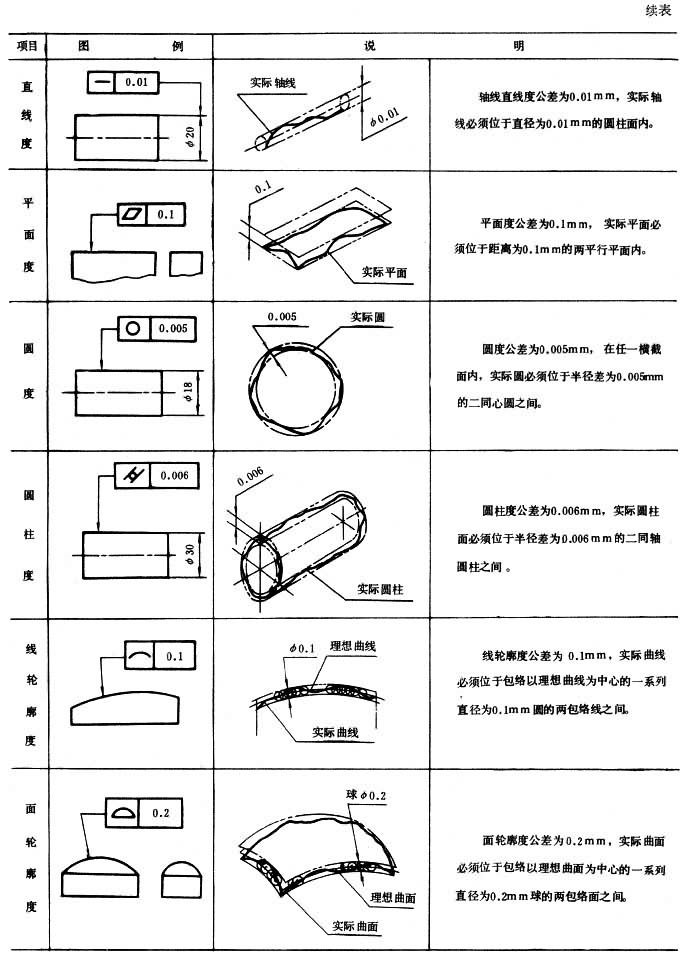
\includegraphics[width=0.9\linewidth]{data/image/13-1}
	\caption{}
%	\label{fig:13-1}
\end{figure}

\begin{figure}[h]
	\centering
	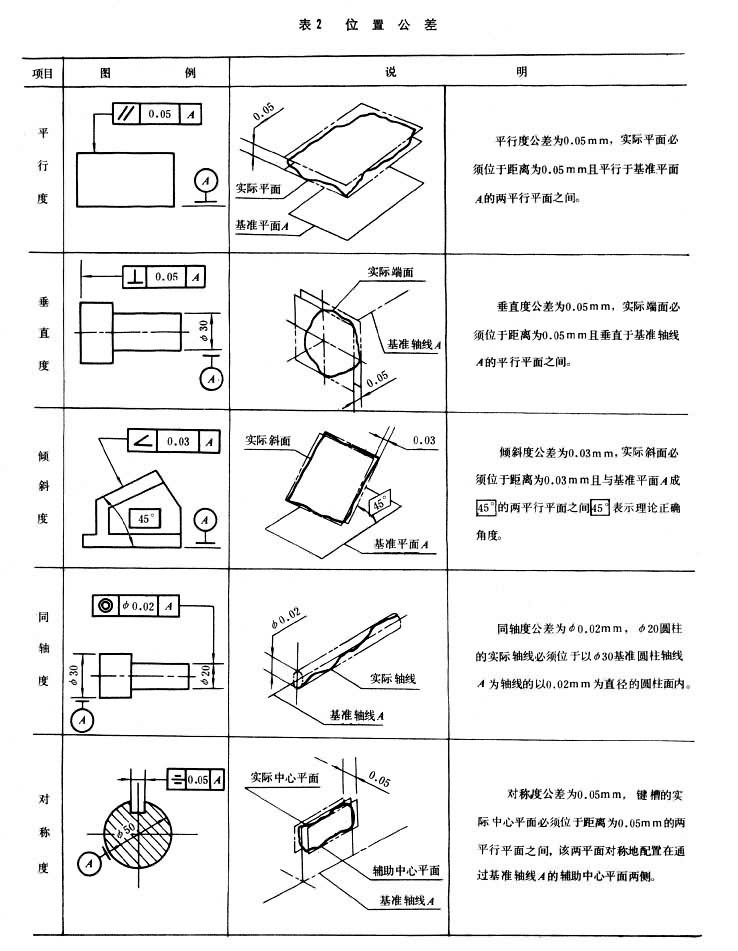
\includegraphics[width=0.9\linewidth]{data/image/13-2}
	\caption{}
%	\label{fig:13-2}
\end{figure}

\begin{figure}[h]
	\centering
	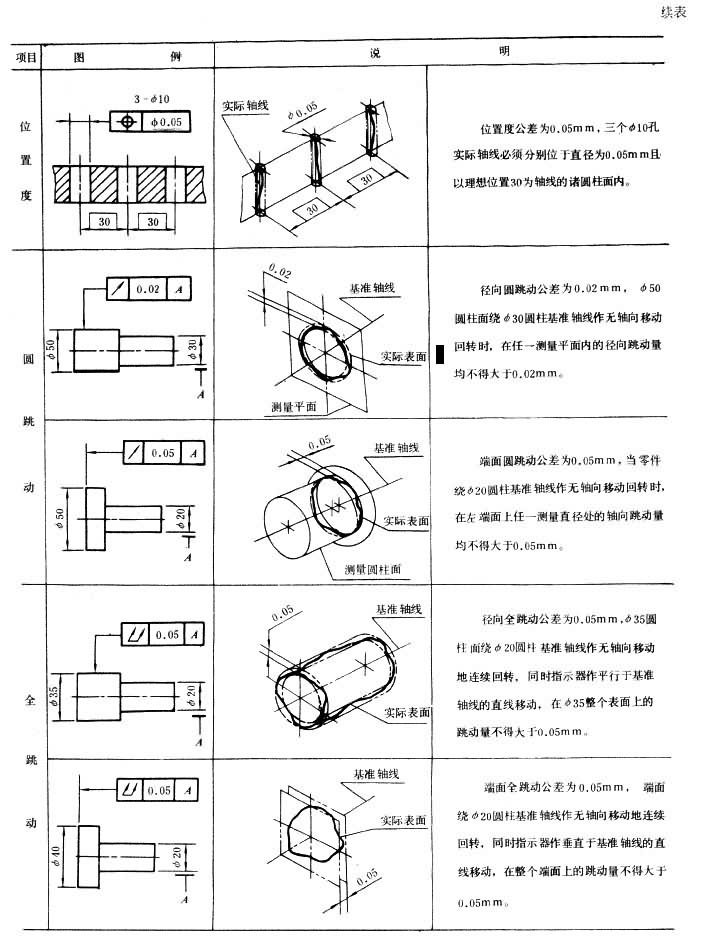
\includegraphics[width=0.9\linewidth]{data/image/13-3}
	\caption{}
%	\label{fig:13-3}
\end{figure}

\subsection{课堂小结}
\begin{enumerate}[1、]
	\item 平面的加工工工艺;
	\item 斜面的加工工艺;
	\item 形位公差;
	\item 编程实例。
\end{enumerate}

\vfill
\subsection{布置作业}
\begin{enumerate}[1、]
	\item 编写斜面的程序。
\end{enumerate}
\vfill
\jxhj{%教学后记
	}
\skrq{%授课日期
	2017年10月31日 4-5节}
\ktmq{%课题名称
	 外轮廓加工}
\jxmb{%教学目标,每行前面要加 \item
	\item 掌握增加刀路去残料的思路;
	\item 掌握增加刀路的方法;
	\item 掌握相关点的计算;
	\item 会合理的增加刀路	。 }
\jxzd{%教学重点,每行前面要加 \item
	\item 增加刀路去残料的思路;
	\item 增加刀路的方法。 }
\jxnd{%教学难点,每行前面要加 \item
	\item 相关点的计算。 }
\jjff{%教学方法
	通过讲述、举例、演示法来说明;}

\makeshouye %制作教案首页

%%%%教学内容
\subsection{组织教学}
\begin{enumerate}[\hspace{2em}1、]
	\item 集中学生注意力;
	\item 清查学生人数;
	\item 维持课堂纪律;
\end{enumerate}

\subsection{复习导入及主要内容}
\begin{enumerate}[1、]
\item 平面的加工工工艺;
\item 斜面的加工工艺;
\item 形位公差;
\item 编程实例。
\end{enumerate}

\subsection{教学内容及过程}
\subsubsection{加工实例}
在数控机床上加工如图\ref{fig:14-1}所示的零件,试完成加工工艺的分析与加工程序的编写,并完加成零件的加工。

\begin{figure}[h]
	\centering
	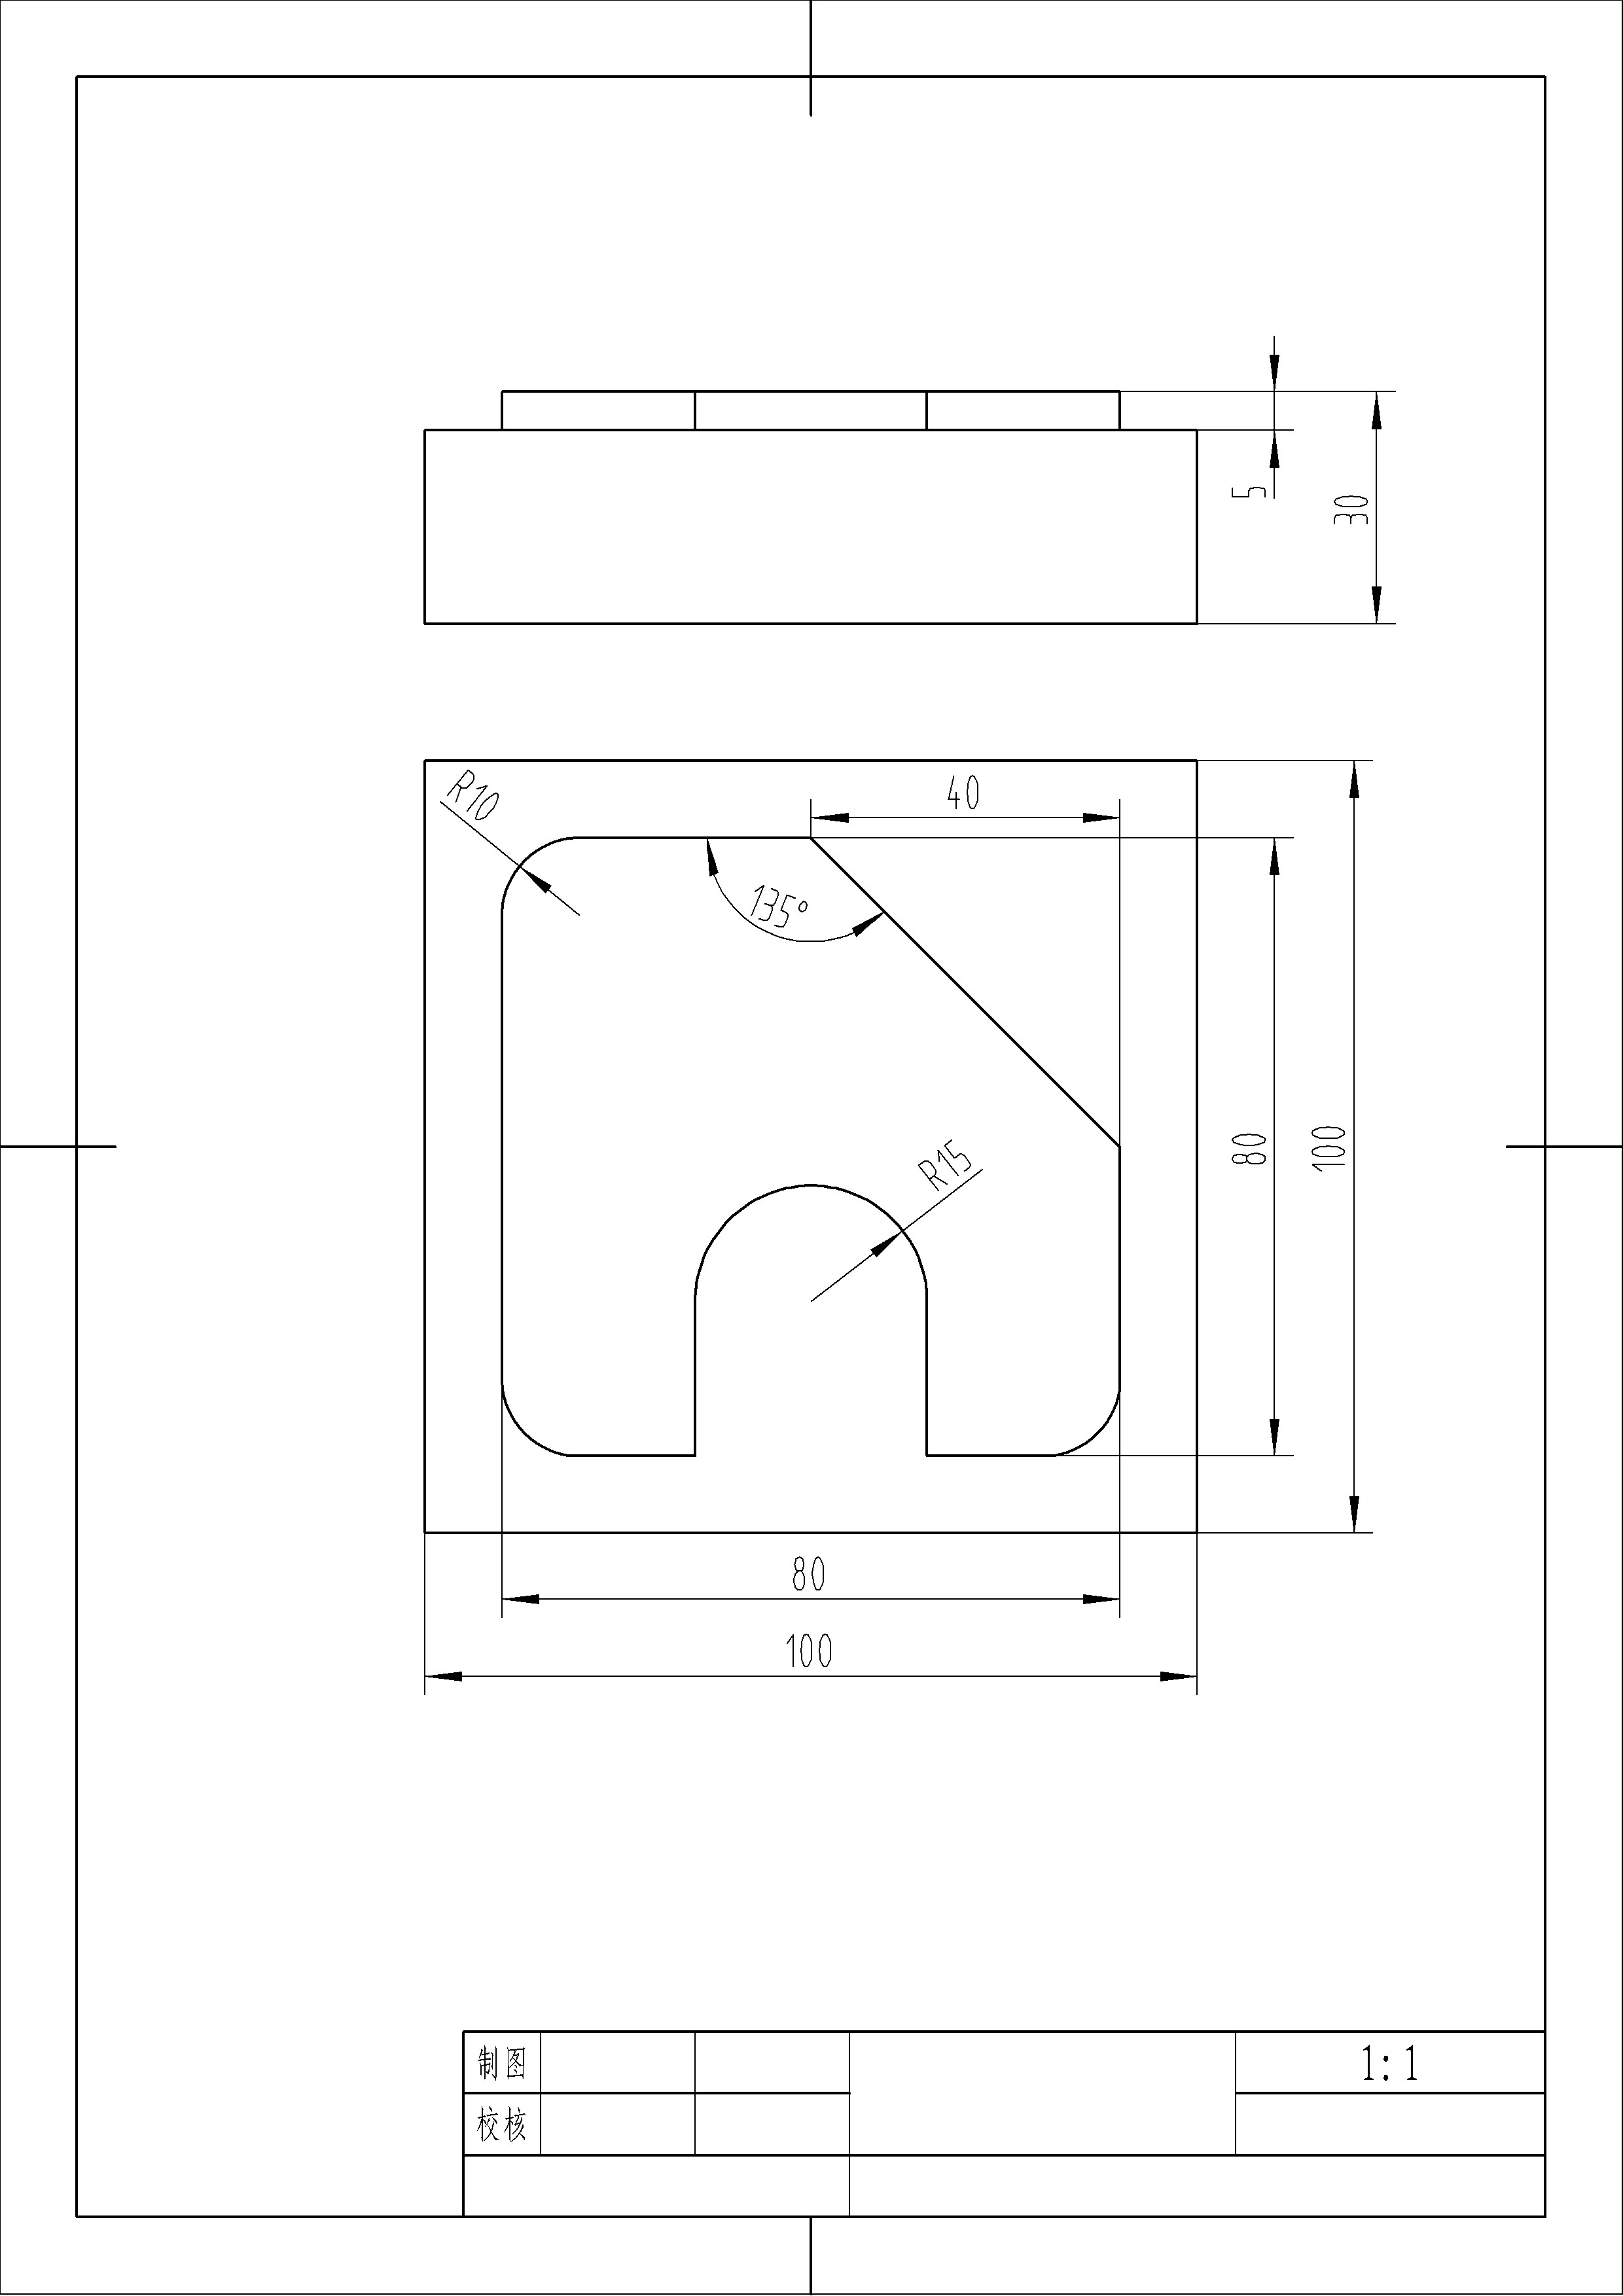
\includegraphics[width=0.8\linewidth,trim=130 200 80  120,clip]{data/image/14-1.jpg}
	\caption{刀补实例}
	\label{fig:14-1}
\end{figure}

1、残料计算:

三个角处的残料为 $20\sqrt{2}-10=18.28$

大角处的残料为  $50\sqrt{2}-20\sqrt{2}=30\sqrt{2}=42.42$

则无论用多大的刀具,此处的残料都不能用刀具半径补偿功能进行去残料。

2、增加刀路去残料:

适合所有类型的去残料,

难点:刀路怎么设计,相关点的计算

基本要求:不能过切,粗加工后能把所有残料去完

自动编程软件:自动计算:

平行往复走刀

沿部件平行环切

沿毛坯平行环切

螺旋高速切削

手工编程:选计算较简单的方法

常用去残料刀路设计:


角

大圆

3、刀路设计:

刀具:铣平面及粗加工:\diameter 12立铣刀

加工宽度10mm

精加工\diameter 10立铣刀

去残料刀路:

角点坐标:

R10--R16.5(粗加工)--R26.5($18.5-16.5=2$)残料去完--改成直线(切线)

$20\sqrt{2}-26.5=2.32$

两边的长:$2.32\sqrt{2} =3.28$

点A(50,-46.)  B(46,-50)

其余根据对称点进行计算

G1 X50. Y-46. 

X46. Y-50.

中间下面的半圆槽:

直线:$C(0,-60) D(0,-20)$


大角:   

$28.28+6.5$ (粗加工) 

$28.28+16.5=44.78$(相当于刀补16.5)

坐标 $ X=50-(70.7-44.78)\sqrt{2} 
=13.349$

$28.28+26.5=54.78 $(相当于刀补26.5)

$X=50-(70.7-54.78)\sqrt{2} 
=27.489$

$28.28+36.6=64.78$(相当于刀补36.5)$+6=42.5$去完

$X=50-(70.7-64.78) \sqrt{2}
=41.629$

G1 X50 Y50

X41.629

X50 Y41.629

Y27.489

X27.489Y50

X13.349

X50 Y13.349

4、程序编写
\begin{lstlisting}

O1(粗加工主程序)
G54G17G40G49G90
M3S500
G1Z20.F2000
X70.Y70.
Z3.0
Z-5. F200
M98P2(去残料)
Z5.0
X0Y60.
Z-5.0
D1M98P3
G1Z30.F2000
M5 
M30
\end{lstlisting}

\begin{lstlisting}
O2(去残料子程序)
N1 G1 X50 Y50
X41.629
X50 Y41.629
Y27.489
X27.489Y50
X13.349
X50 Y13.349
X60.
N2 Y-46.
X50.
X46.Y-50.
Y-60
N3X-46.
Y-50.
X-50.Y-46.
Y-60.
N4 Y46.
X-50
X-46.Y50.
Y60.
M99;
\end{lstlisting}

\begin{lstlisting}
O3(轮廓子程序)
G1X-10.Y50.
G3X0Y40.R10.
G1X40.Y0
G1Y-30.
...

...

\end{lstlisting}












\begin{lstlisting}
O4(精加工主程序)
G54G17G40G49G90
M3S800
G1Z20.F2000
X0.Y60.
Z3.0
Z-5. F200
Z-5.0
D1M98P3
G1Z30.F2000
M5 
M30
\end{lstlisting}




\subsection{课堂小结}
\begin{enumerate}[1、]
	\item 增加刀路去残料;
	\item 加工实例;
	\item 相关计算。
\end{enumerate}

\vfill
\subsection{布置作业}
\begin{enumerate}[1、]
	\item 编写上面的程序。
\end{enumerate}
\vfill
\jxhj{%教学后记
	}
\skrq{%授课日期
	2017年11月2日 4-5节}
\ktmq{%课题名称
	 期中考试}
\jxmb{%教学目标,每行前面要加 \item
	\item 期中考试}
\jxzd{%教学重点,每行前面要加 \item
	\item 期中考试。}
\jxnd{%教学难点,每行前面要加 \item
	\item 期中考试。}
\jjff{%教学方法
	期中考试;}

\makeshouye %制作教案首页

%%%%教学内容
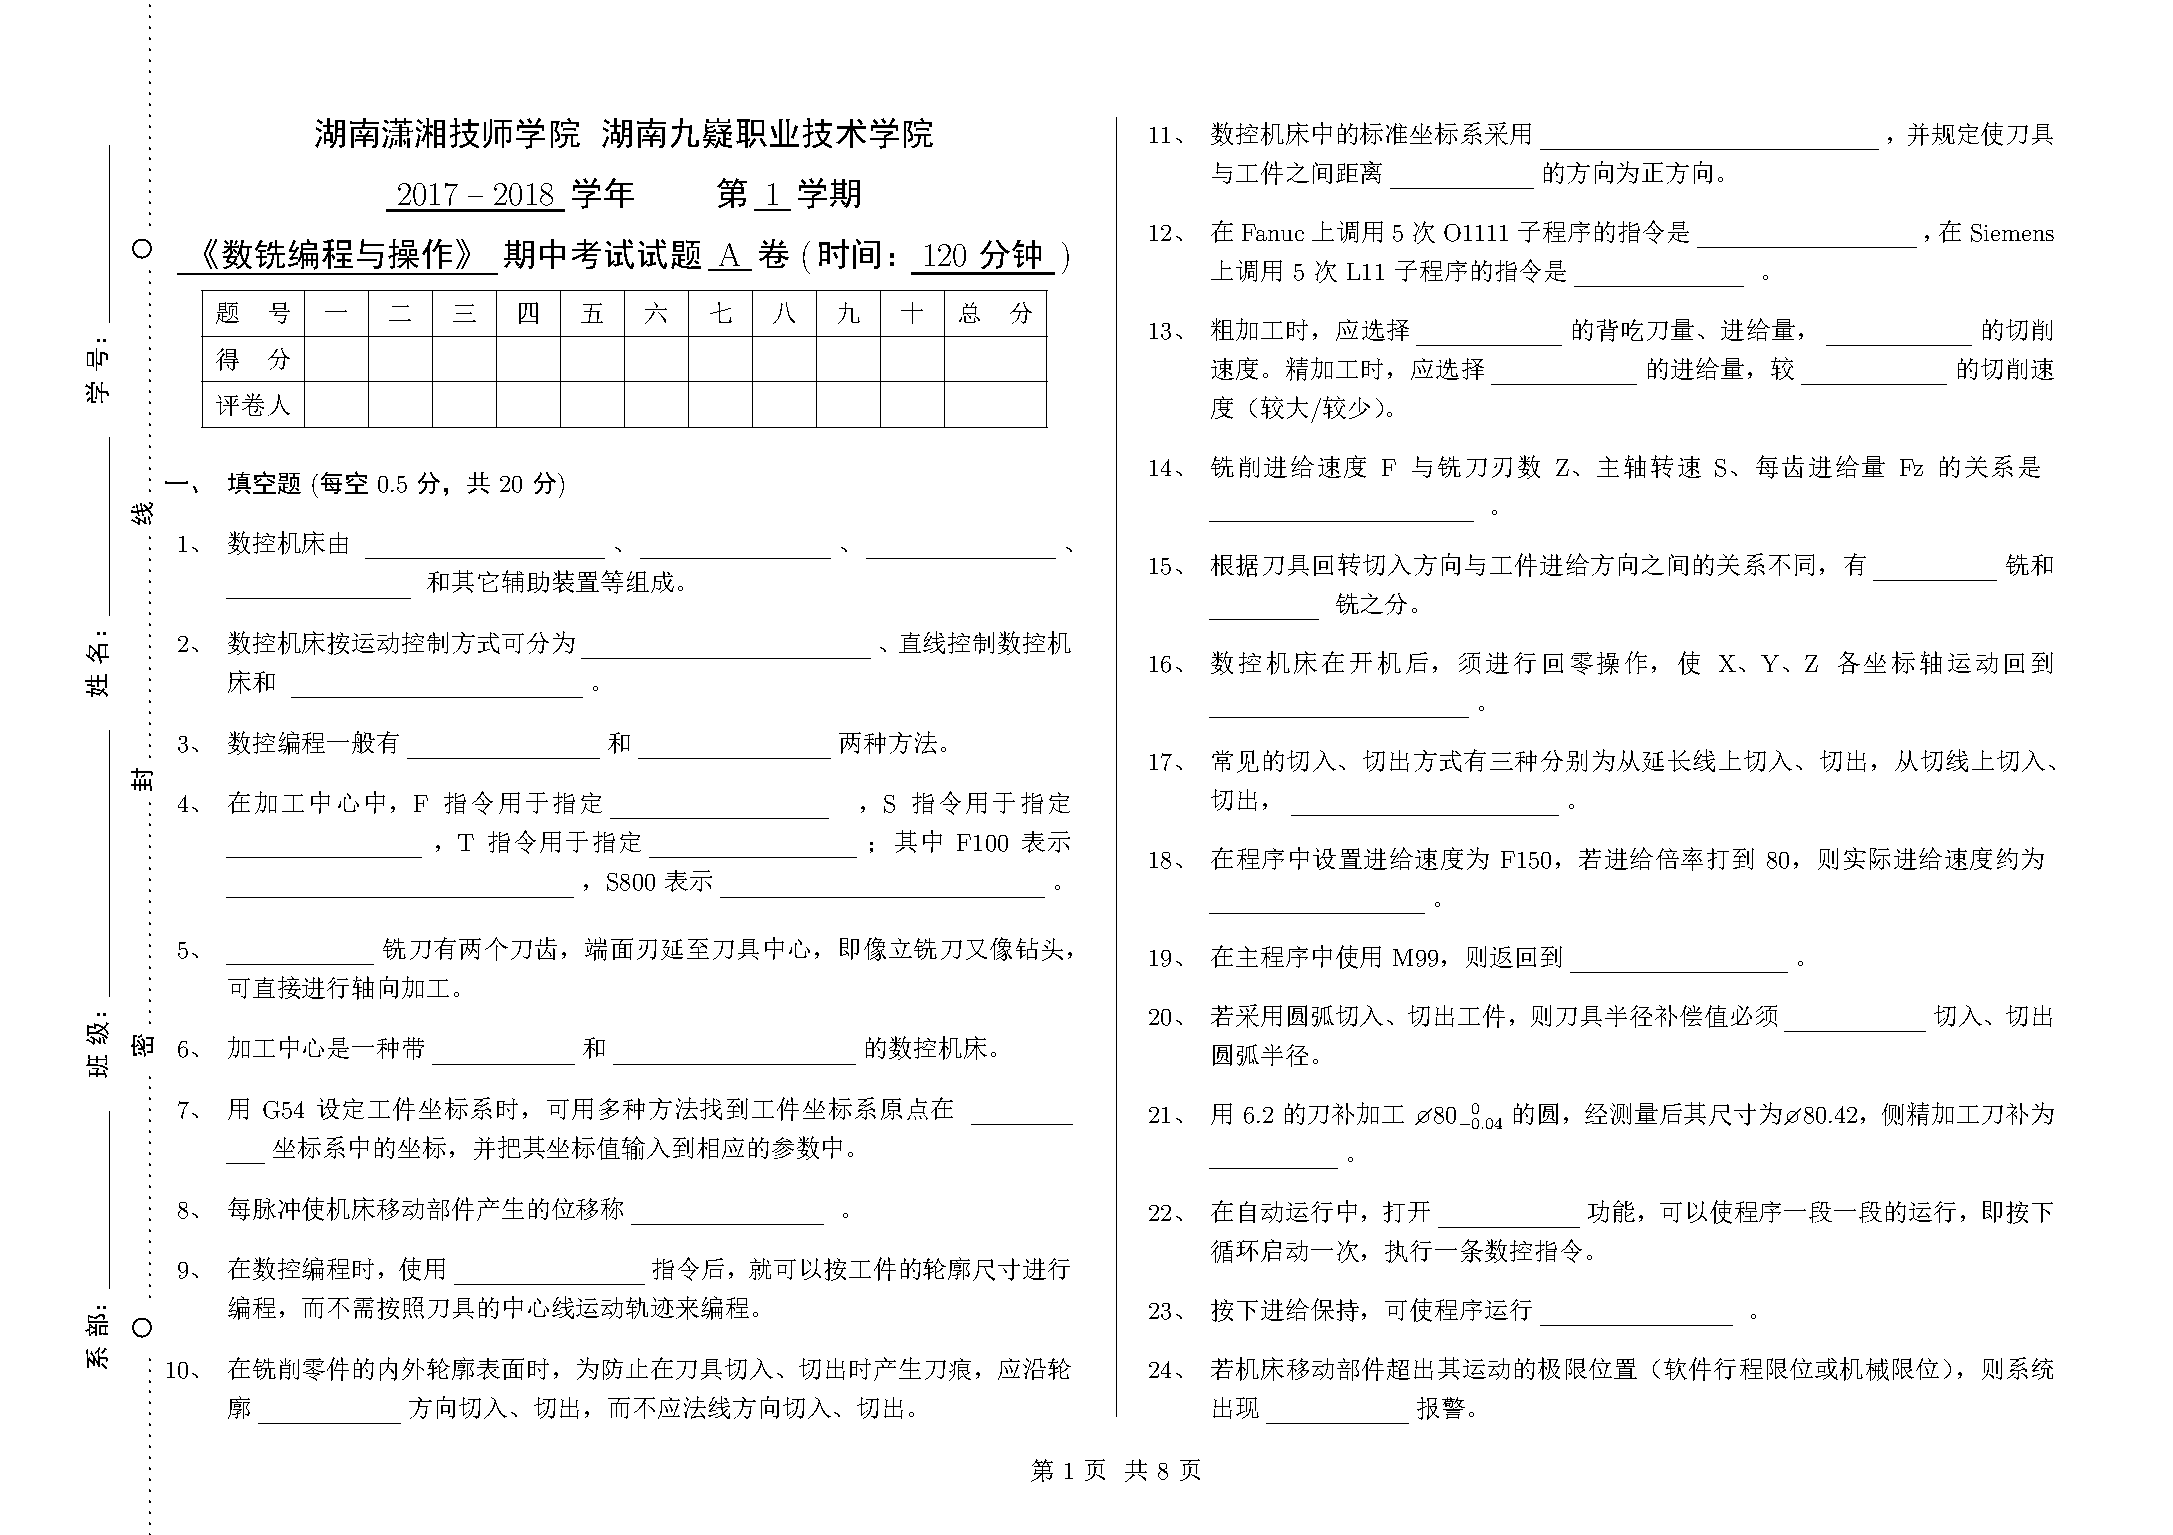
\includepdf[pages={-},landscape=true]{shijuan.pdf}
\jxhj{%教学后记
	}
\skrq{%授课日期
	2017年11月7日 4-5节}
\ktmq{%课题名称
	 期中考试讲解}
\jxmb{%教学目标,每行前面要加 \item
	\item 复习巩固}
\jxzd{%教学重点,每行前面要加 \item
	\item 复习巩固。}
\jxnd{%教学难点,每行前面要加 \item
	\item 复习巩固。}
\jjff{%教学方法
	复习巩固;}

\makeshouye %制作教案首页

%%%%教学内容
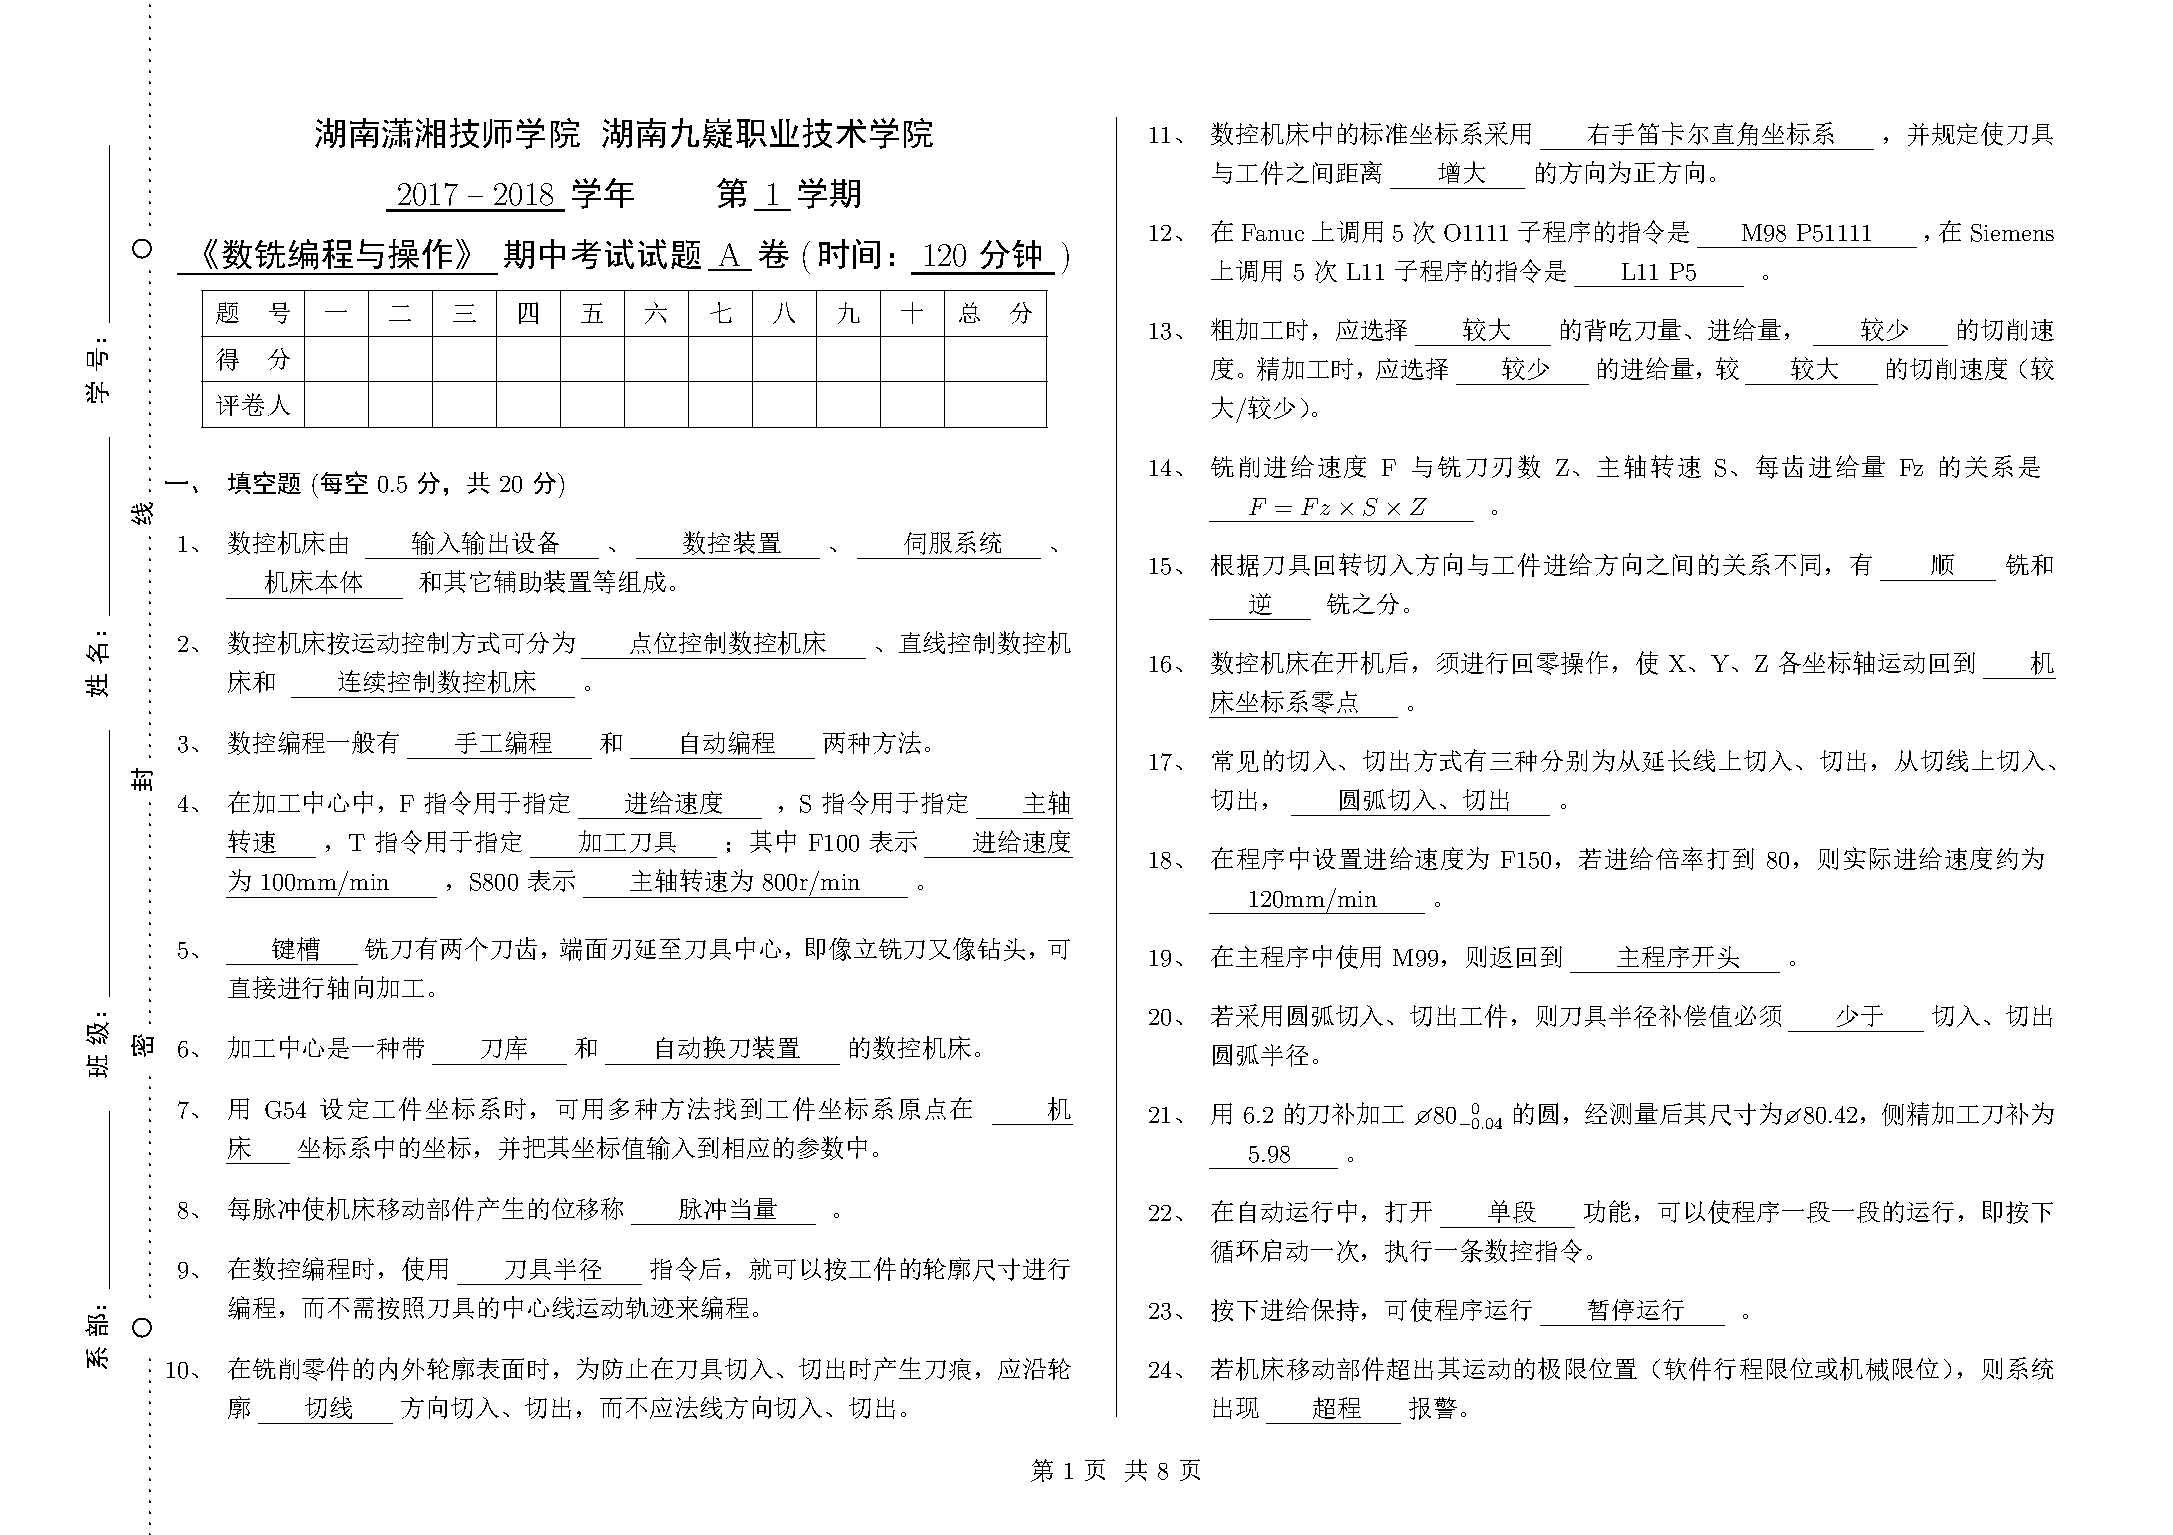
\includepdf[pages={-},landscape=true]{shijuan-daan.pdf}
\jxhj{%教学后记
	}
\skrq{%授课日期
	2017年11月9日 4-5节}
\ktmq{%课题名称
	 型腔加工}
\jxmb{%教学目标,每行前面要加 \item
	\item 掌握挖槽加工的工艺;
	\item 掌握挖槽加工的下刀方式;
	\item 会写简单的挖槽程序。}
\jxzd{%教学重点,每行前面要加 \item
	\item 挖槽加工的工艺;
	\item 写简单的挖槽程序。 }
\jxnd{%教学难点,每行前面要加 \item
	\item 写简单的挖槽程序。 }
\jjff{%教学方法
	通过讲述、举例、演示法来说明;}

\makeshouye %制作教案首页

%%%%教学内容
\subsection{组织教学}
\begin{enumerate}[\hspace{2em}1、]
	\item 集中学生注意力;
	\item 清查学生人数;
	\item 维持课堂纪律;
\end{enumerate}

\subsection{复习导入及主要内容}
\begin{enumerate}[1、]
\item 增加刀路去残料;
\item 加工实例;
\item 相关计算。
\end{enumerate}

\subsection{教学内容及过程}
\subsubsection{刀具的选择}
要求:有底刃和侧刃(即键槽铣刀)两条侧刃

但粗加工还是可以用立铣刀,(要先加工工艺孔)

\subsubsection{下刀方式}
1、直接下刀:一轴移动(预钻孔) 

G01 Z\_\_ F(10-20);

2、斜线下刀:两轴移动(狭长地带)

G01 Z\_\_ X\_\_ / Y\_\_ F(30-40)

3、螺线下刀:三轴移动(空间较大)

G17 G02/G03 X\_\_ Y\_\_ Z\_\_ I\_\_ J\_\_ / R\_\_ F\_\_

指令要写全,不能省。

\subsubsection{斜线下刀}

1、坡度3°\~ 5°

即:移动10mm下刀约1mm

2、长度不够:

可采用Z字形下刀

3、斜坡铣削:

G01 X\_\_ Z\_\_ F\_\_

X\_\_  (返回)

\subsubsection{去材料方式}

1、往复铣削(如铣长方形)

2、环形(如铣圆形,正方形)

3、少用刀补来去材料

\subsubsection{圆形槽铣削}

利用数控铣床加在\diameter 110*35的毛坯上加工\diameter 100*5的槽。毛坯材料为45号钢,上表面未加工。按图样要求完成零件的节点、基点、辅助点计算。设定工件坐标系,制定正确的工艺方案(包括定位,夹紧方案和工艺路线),选择合理的刀具和切削工艺参数,编写数控加工程序。

1、工艺分析:

零件简单,尺寸精度均达到IT8-IT7级

采用机用平口钳装夹,两侧面先工艺平面用于装夹

工件坐标系原点设在铣好的上表面中心

工序:平面

挖槽:

2、刀具选择:

平面用\diameter 80可转位铣刀,

挖槽:粗加工用\diameter 14三刃立铣刀

精加工用\diameter 12四刃立铣刀

3、刀削参数的选择:

{\noindent
    
     \begin{figure}[!hbtp]
        \centering
        \footnotesize
        %\hspace{-3.4ex}
        \renewcommand\arraystretch{1.9}
\begin{tabu}to 0.6\textwidth{|c|c|c|c|c|c|c|c|}
    \hline 
    序号 & 加工 & 刀具类型 & 刀具 & 主轴 & 进给& 长度 & 半径 \\ 
    & 内容 &  & 材料 & 转速 & 速度 & 补偿 & 补偿 \\
    \hline 
    1 & 粗加工上表面 & \diameter 可转位铣刀 & 硬质合金 & 500 & 250 &  &  \\ 
    \hline 
    2&精加工上表面& \diameter 可转位铣刀  & 硬质合金 &800  &160  &  &  \\ 
    \hline 
    3&粗加工槽  & \diameter 14立铣刀 &高速钢  &500  &80  &  &7.2  \\ 
    \hline 
    4&精加工槽  & \diameter 12立铣刀 &高速钢  &800  &80  &  &5.985  \\ 
    \hline 
\end{tabu} 
\end{figure}}

4、走刀路径

粗加工刀补:7.2  R0=42.8

去残料圆半径   R1=35

R2=27

R3=19

R4=11

5、参考程序

\begin{lstlisting}
O0001;(粗加工)
G54 G17 G40 G49 G90;
M03 S500;
G01 Z30.0 F100;
X-42.8 Y0;
Z0.5;
G01 X42.8 Z-5.0 F40;
X-42.8 F80;
X-11.0;
G02 I11.0;
G01 X-19.0;
G02 I19.0;
G01 X-27.0;
G02 I-27.0;
G01 X-35;
G02 I35.0;
G01 X-42.8; 
G02 I42.8;
G0 Z30.0;
M05;
M30;
\end{lstlisting}

\begin{lstlisting}
O0002;(精加工)
G54 G17 G40 G49 G90
M03 S800
G01 Z30.0 F100
XO Y0
Z-5.0
G01 G41 X40.0 Y-10.0 D1 
G03 X50.0 Y0 R10.0
G03 I50.0
G03 X40.0 Y10.0 R10.0
G40 G01 X0 Y0
Z30.0
M05
M30
\end{lstlisting}

\subsection{课堂小结}
\begin{enumerate}[1、]
	\item 刀具的选择;
	\item 下刀方式;
	\item 斜线下刀;
    \item 去残料方式;
    \item 圆形槽铣削加工实例。
\end{enumerate}

\vfill
\subsection{布置作业}
\begin{enumerate}[1、]
	\item 编写圆形槽的程序。
\end{enumerate}
\vfill
\jxhj{%教学后记
	}
\skrq{%授课日期
	2017年11月14日 4-5节}
\ktmq{%课题名称
	 型腔加工}
\jxmb{%教学目标,每行前面要加 \item
	\item 掌握型腔加工的下刀方式;
    \item 掌握矩形槽去残料的方式;
    \item 会用G91斜线下刀及Z向分层;
    \item 会编写矩形槽的程序。}
\jxzd{%教学重点,每行前面要加 \item
	\item 用G91斜线下刀及Z向分层;
	\item 编写矩形槽的程序。 }
\jxnd{%教学难点,每行前面要加 \item
	\item 编写矩形槽的程序。 }
\jjff{%教学方法
	通过讲述、举例、演示法来说明;}

\makeshouye %制作教案首页

%%%%教学内容
\subsection{组织教学}
\begin{enumerate}[\hspace{2em}1、]
	\item 集中学生注意力;
	\item 清查学生人数;
	\item 维持课堂纪律;
\end{enumerate}

\subsection{复习导入及主要内容}
\begin{enumerate}[1、]
\item 刀具的选择;
\item 下刀方式;
\item 斜线下刀;
\item 去残料方式;
\item 圆形槽铣削加工实例。
\end{enumerate}

\subsection{教学内容及过程}
\subsubsection{方形槽铣削}
利用数控铣床加在\diameter 110*35的毛坯上加工80*60深5mm的方槽。毛坯材料为45号钢,上表面未加工。按图样要求完成零件的节点、基点、辅助点计算。设定工件坐标系,制定正确的工艺方案(包括定位,夹紧方案和工艺路线),选择合理的刀具和切削工艺参数,编写数控加工程序。

\begin{figure}[h]
	\centering
	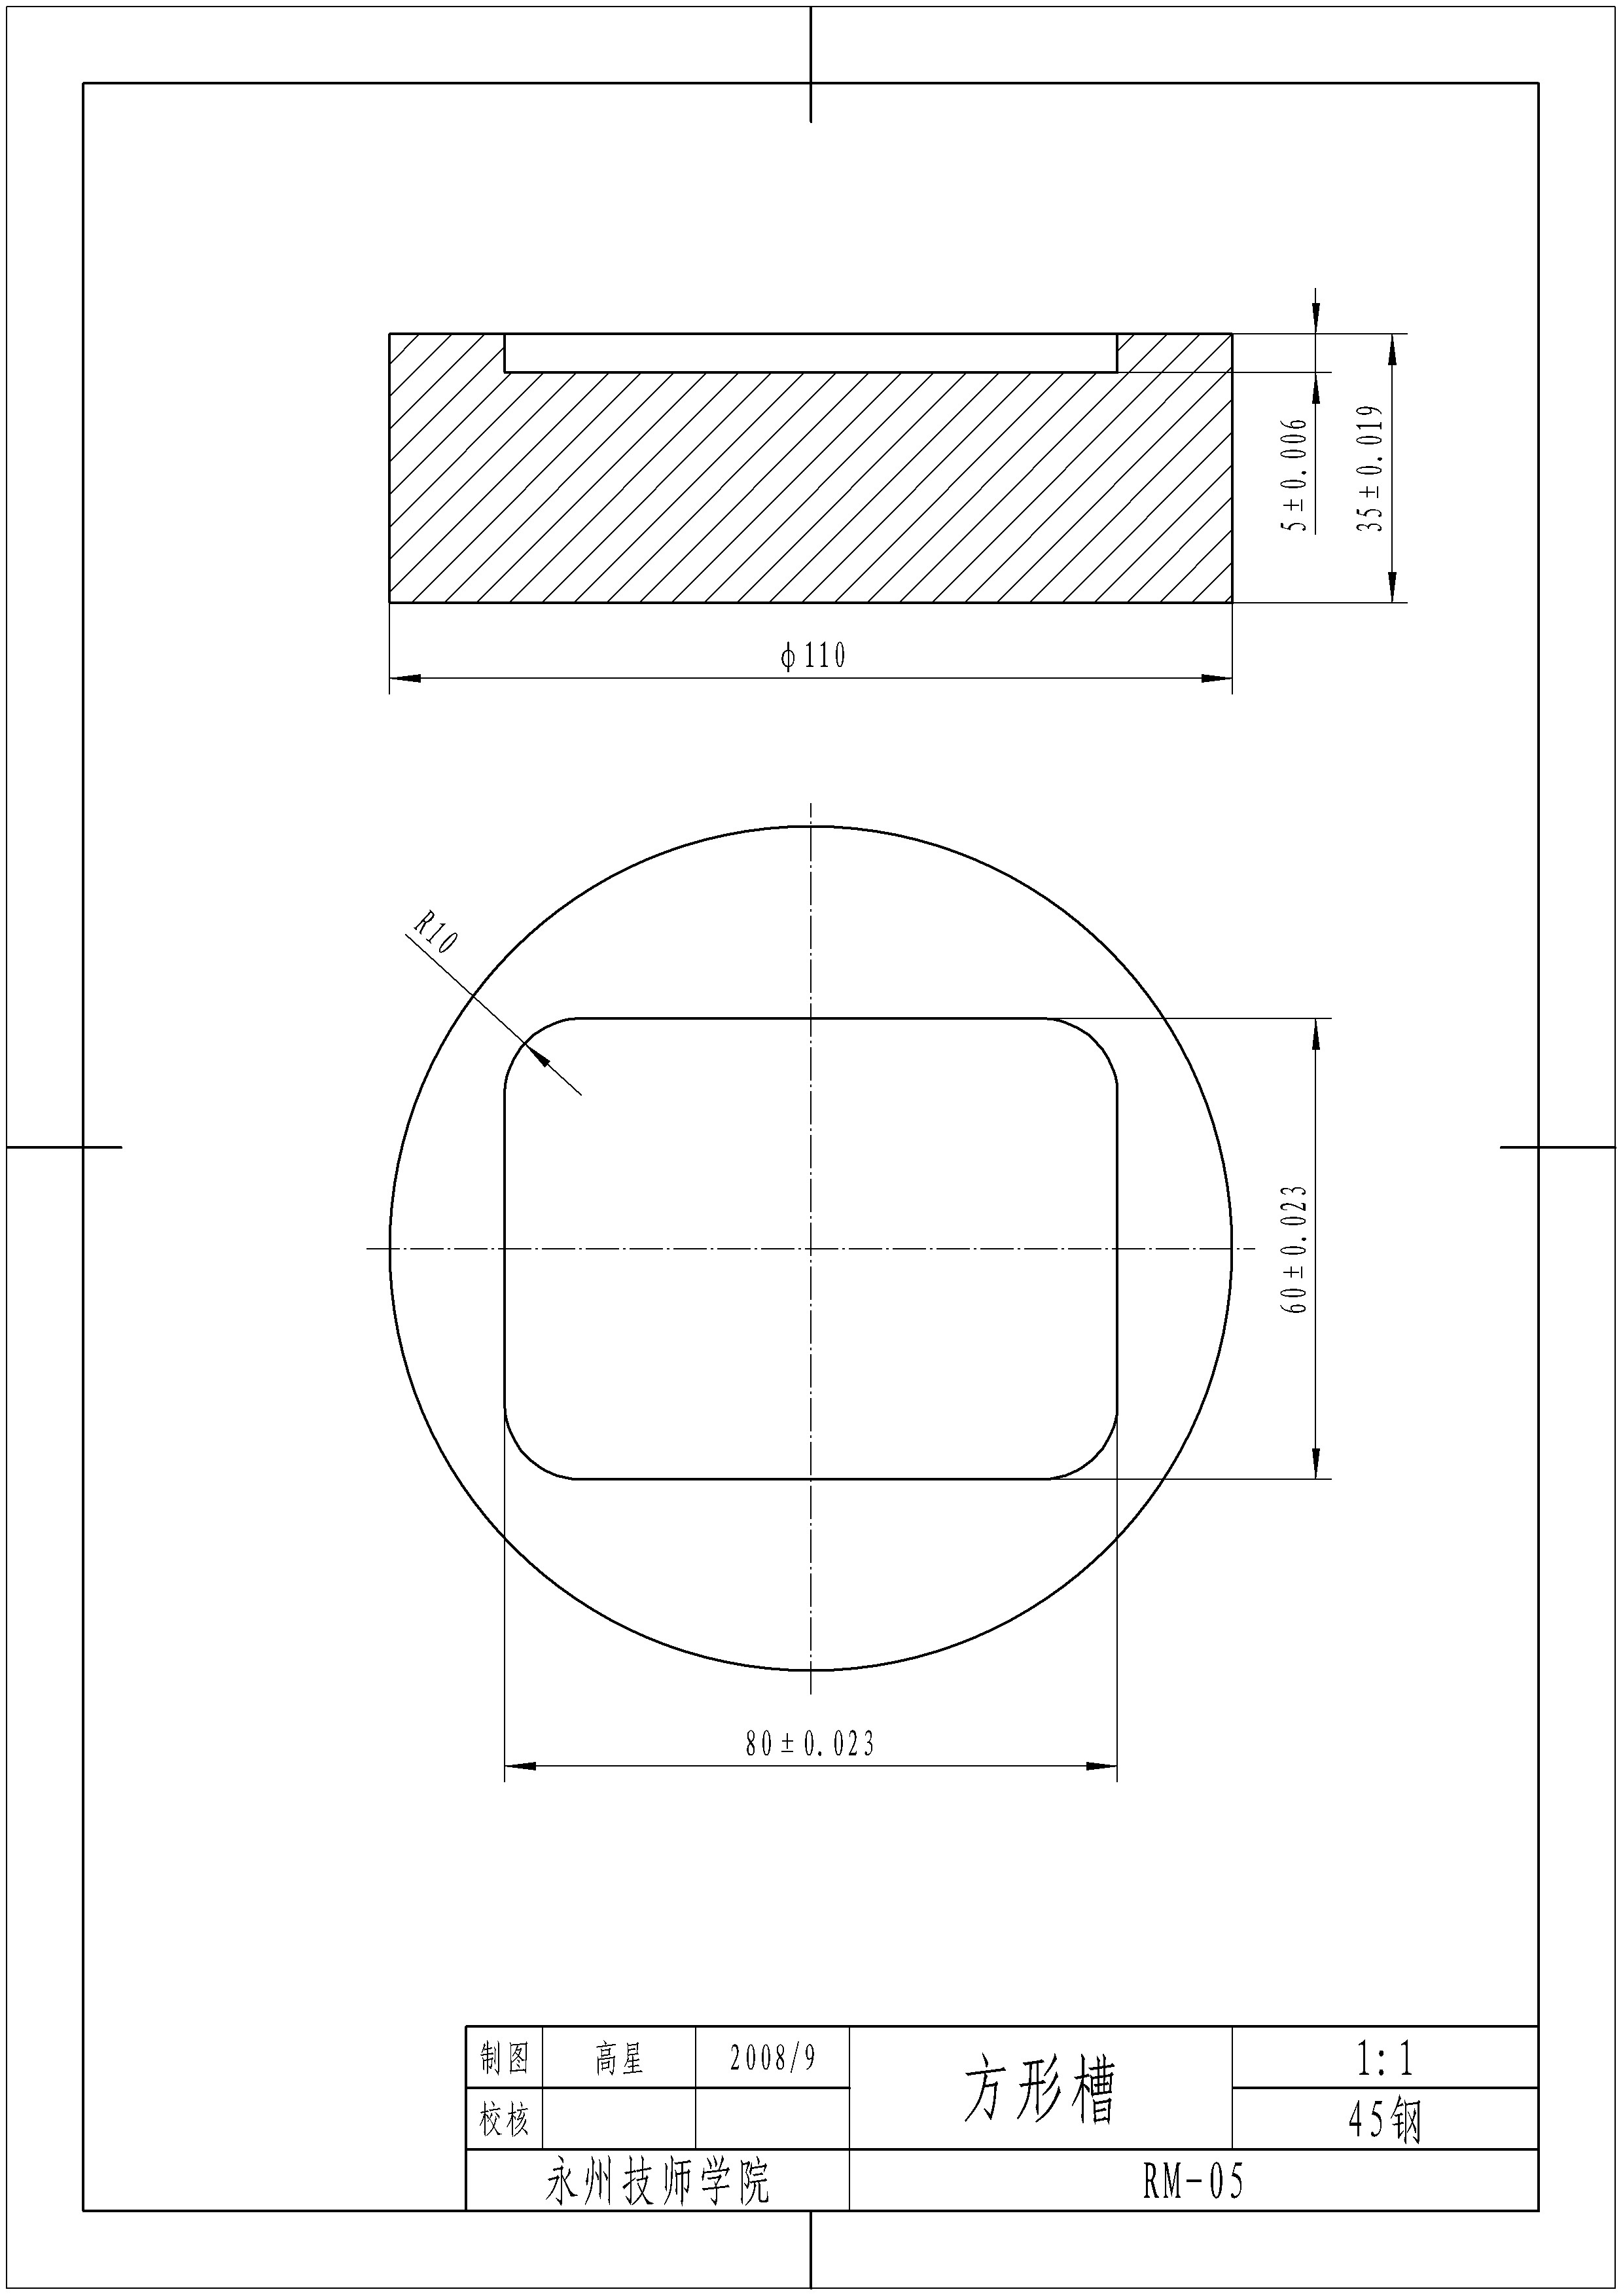
\includegraphics[width=0.8\linewidth,trim=130 180 80  120,clip]{data/image/18-1.jpg}
	\caption{方形槽铣削}
	\label{fig:18-1}
\end{figure}

1、工艺分析:

零件简单,尺寸精度均达到IT8-IT7级

采用机用平口钳装夹,两侧面先工艺平面用于装夹

工件坐标系原点设在铣好的上表面中心

工序:平面

挖槽:

2、刀具选择:

平面用\diameter 80可转位铣刀,

挖槽:粗加工用\diameter 14三刃立铣刀

精加工用\diameter 12四刃立铣刀

3、刀削参数的铣铣择:

{\noindent
    
    \begin{figure}[!hbtp]
        \centering
        \footnotesize
        %\hspace{-3.4ex}
        \renewcommand\arraystretch{1.9}
        \begin{tabu}to 0.6\textwidth{|c|c|c|c|c|c|c|c|}
            \hline 
            序号 & 加工 & 刀具类型 & 刀具 & 主轴 & 进给& 长度 & 半径 \\ 
            & 内容 &  & 材料 & 转速 & 速度 & 补偿 & 补偿 \\
            \hline 
            1 & 粗加工上表面 & \diameter 可转位铣刀 & 硬质合金 & 500 & 250 &  &  \\ 
            \hline 
            2&精加工上表面& \diameter 可转位铣刀  & 硬质合金 &800  &160  &  &  \\ 
            \hline 
            3&粗加工槽  & \diameter 14立铣刀 &高速钢  &500  &80  &  &7.2  \\ 
            \hline 
            4&精加工槽  & \diameter 12立铣刀 &高速钢  &800  &80  &  &5.985  \\ 
            \hline 
        \end{tabu} 
\end{figure}}

4、走刀路径

粗加工刀补:7.2  

5、参考程序

\begin{lstlisting}
O1;
G54G17G90G40;
M3S400;
G1Z100.0F2000;
X-30.0Y20.0;
Z5.0;
G1Z0F150.0;
M98P2;
G1Z100.0F2000;
M5;
M30;
\end{lstlisting}

\begin{lstlisting}
O2;
G91G1X60.0Z-5.0F40;
X-60.0F150;
M98P200;
G90G1X25.0Y0
D1M98P2000
G1X-30.0Y20.0
M99
\end{lstlisting}
\begin{lstlisting}
O200;
G91G1Y-12.0
X60.0
Y-12.0
X-60.0
Y-12.0
X60.0;
Y-4.0
X-60.0
M99
\end{lstlisting}
\begin{lstlisting}
O2000;
G1G41X30.0Y10.0
G3X40.0Y0R10.0
G1Y20.0
G3X30.0Y30.0R10.0
G1Y-20.0
G3X-30.0Y-30.0R10.0
G1X30.0
G3X40.0Y-20.0
G1Y0
G3X30.0Y10.0R10.0
G1G40X25.0Y0
M99
\end{lstlisting}
课堂练习:
如果加工深度为12mm,怎样写程序:
\begin{figure}[h]
    \centering
    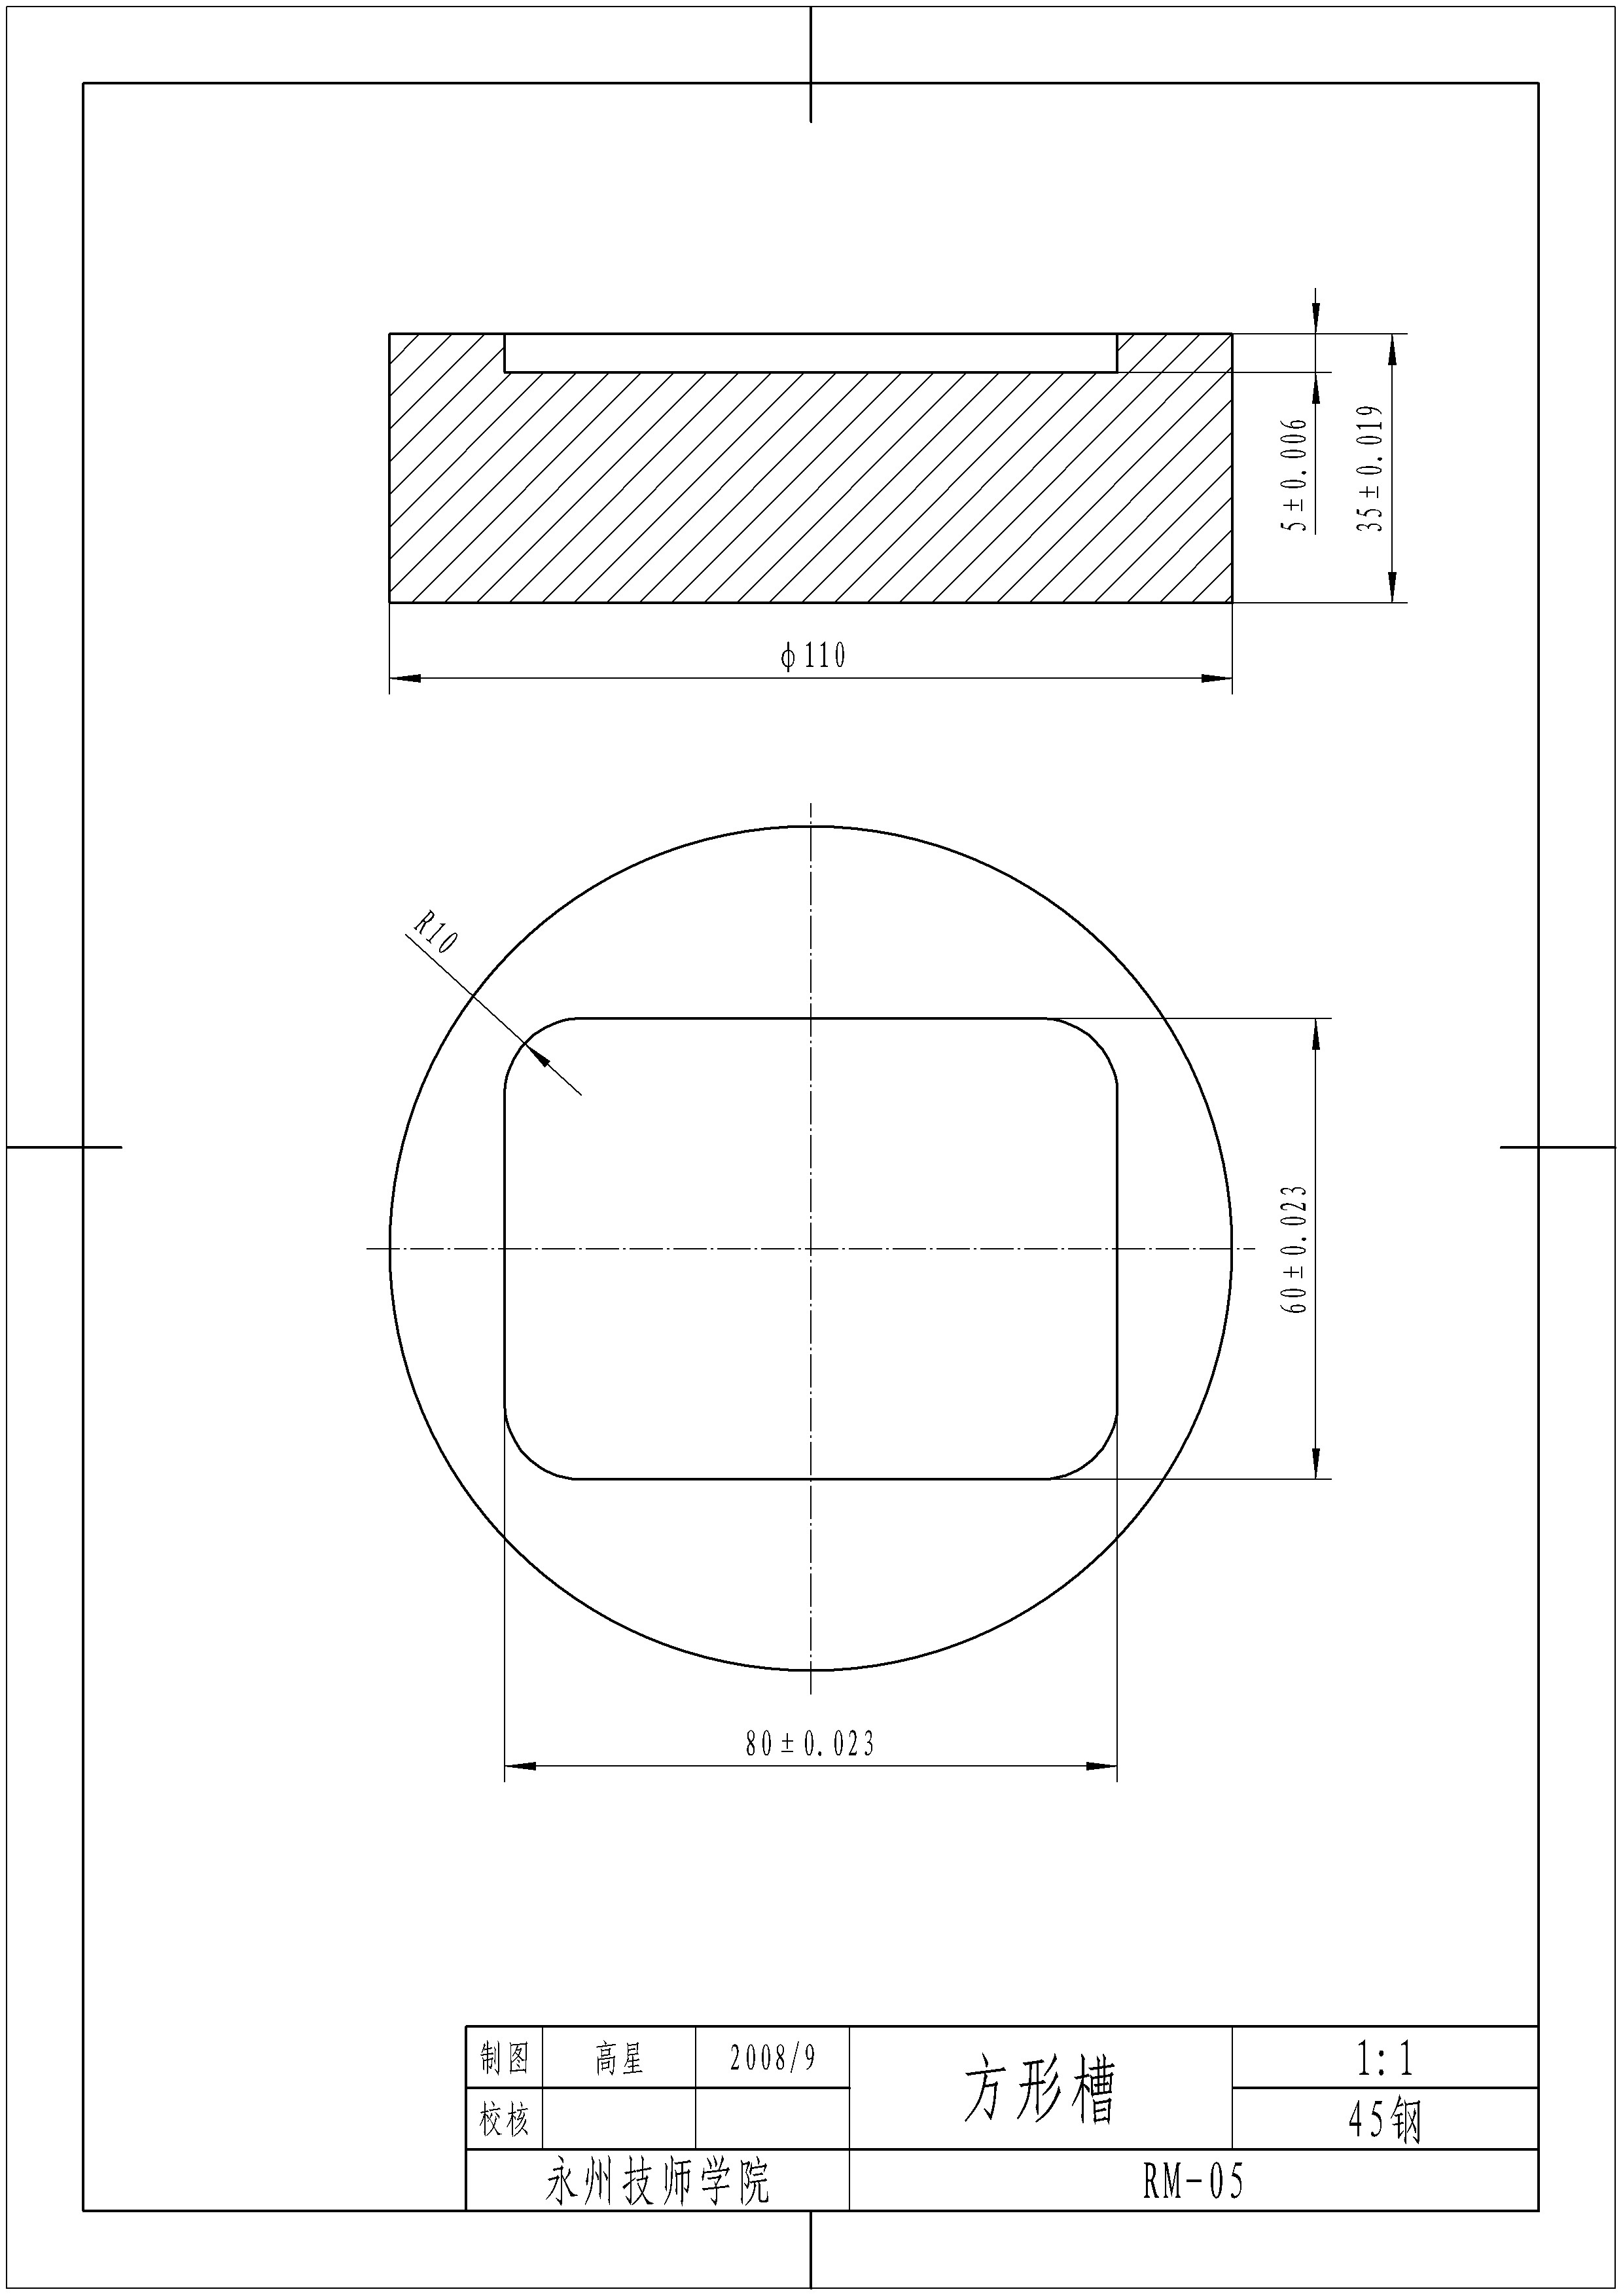
\includegraphics[width=0.8\linewidth,trim=130 180 80  120,clip]{data/image/18-1.jpg}
    \caption{方形槽铣削,深度改为12mm}
    \label{fig:18-2}
\end{figure}


\subsection{课堂小结}
\begin{enumerate}[1、]
\item 刀具的选择;
\item 下刀方式;
\item 斜线下刀;
\item 去残料方式;
\item 方槽铣削加工实例。
\end{enumerate}

\vfill
\subsection{布置作业}
\begin{enumerate}[1、]
	\item 编写上面的程序。
\end{enumerate}
\vfill
\jxhj{%教学后记
	}
\skrq{%授课日期
	2017年11月16日 4-5节}
\ktmq{%课题名称
	 岛屿型腔加工}
\jxmb{%教学目标,每行前面要加 \item
	\item 掌握岛屿型腔加工的下刀方式;
    \item 掌握岛屿槽去残料的方式;
    \item 会用G91螺线下刀及Z向分层;
    \item 会编写岛屿型腔的程序。}
\jxzd{%教学重点,每行前面要加 \item
	\item 编写岛屿型腔的程序;
	\item G91螺线下刀及Z向分层。 }
\jxnd{%教学难点,每行前面要加 \item
	\item 编写岛屿型腔的程序。 }
\jjff{%教学方法
	通过讲述、举例、演示法来说明;}

\makeshouye %制作教案首页

%%%%教学内容
\subsection{组织教学}
\begin{enumerate}[\hspace{2em}1、]
	\item 集中学生注意力;
	\item 清查学生人数;
	\item 维持课堂纪律;
\end{enumerate}

\subsection{复习导入及主要内容}
\begin{enumerate}[1、]
\item 刀具的选择;
\item 下刀方式;
\item 斜线下刀;
\item 去残料方式;
\item 方槽铣削加工实例。
\end{enumerate}

\subsection{教学内容及过程}
\subsubsection{加工实例}
实例:用数控铣完成如图10-1所示零件的加式工。零件材料为45号钢,毛坯为\diameter 110×35mm。按图样要求完成零件基点及辅助点的计算,设定工件坐标系,制定正确的工艺方案(包括定位、夹紧方案和工艺路线),选择合理的刀具和切削工艺参数,编制数控加工程序。

\begin{figure}[h]
	\centering
	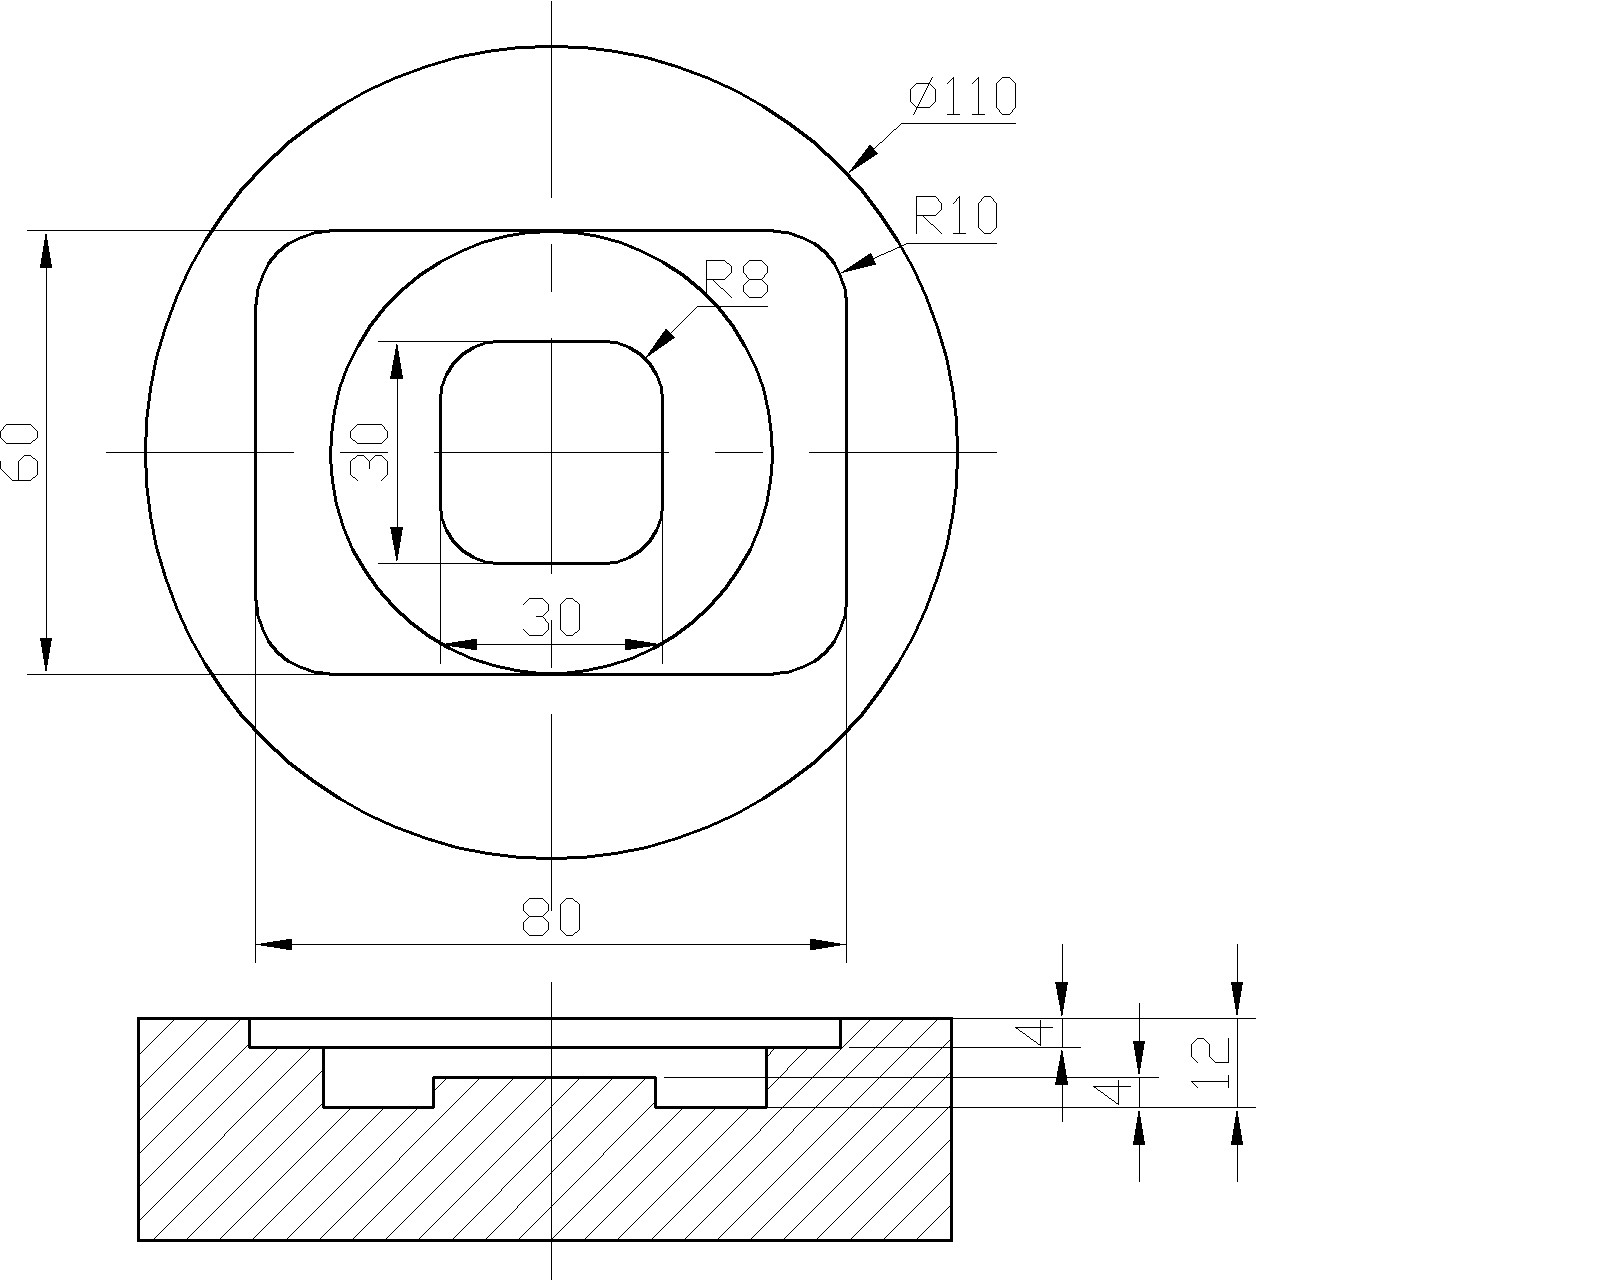
\includegraphics[width=0.8\linewidth,trim=0 0 150  0,clip]{data/image/19-1.jpg}
	\caption{岛屿型腔加工}
	\label{fig:19-1}
\end{figure}

\subsubsection{刀具选择及工艺路线}
1、工艺分析

此工件毛坯加工完成,只要进行槽的加工,且所有精度一样,没有其它要求。零件的装夹采用平口钳装夹。将工件坐标系G54建立在工件上表面、零件的对称中心。针对零件图样要求给出加工工序为:

(1)用Z向分两层加工φ60*8的槽

(2)加工中间的岛屿

(3)用刀补加工长方形的槽。

2、刀具的选择

最小内凹圆弧半径为R10,且岛屿间的最小间距约为12mm,故粗加工用φ10的立铣刀。精加工用φ10的立铣刀。

3、切削参数的选择

粗加工   S500   F100

精加工   S800   F80

粗加工补 D1=5.5

精加工补 D2=(计算所得)

4、加工路径:

(1)螺旋下刀:

为使岛屿共用一个下刀,用R24的圆弧螺旋下刀,如图所示:

\begin{figure}[h]
    \centering
    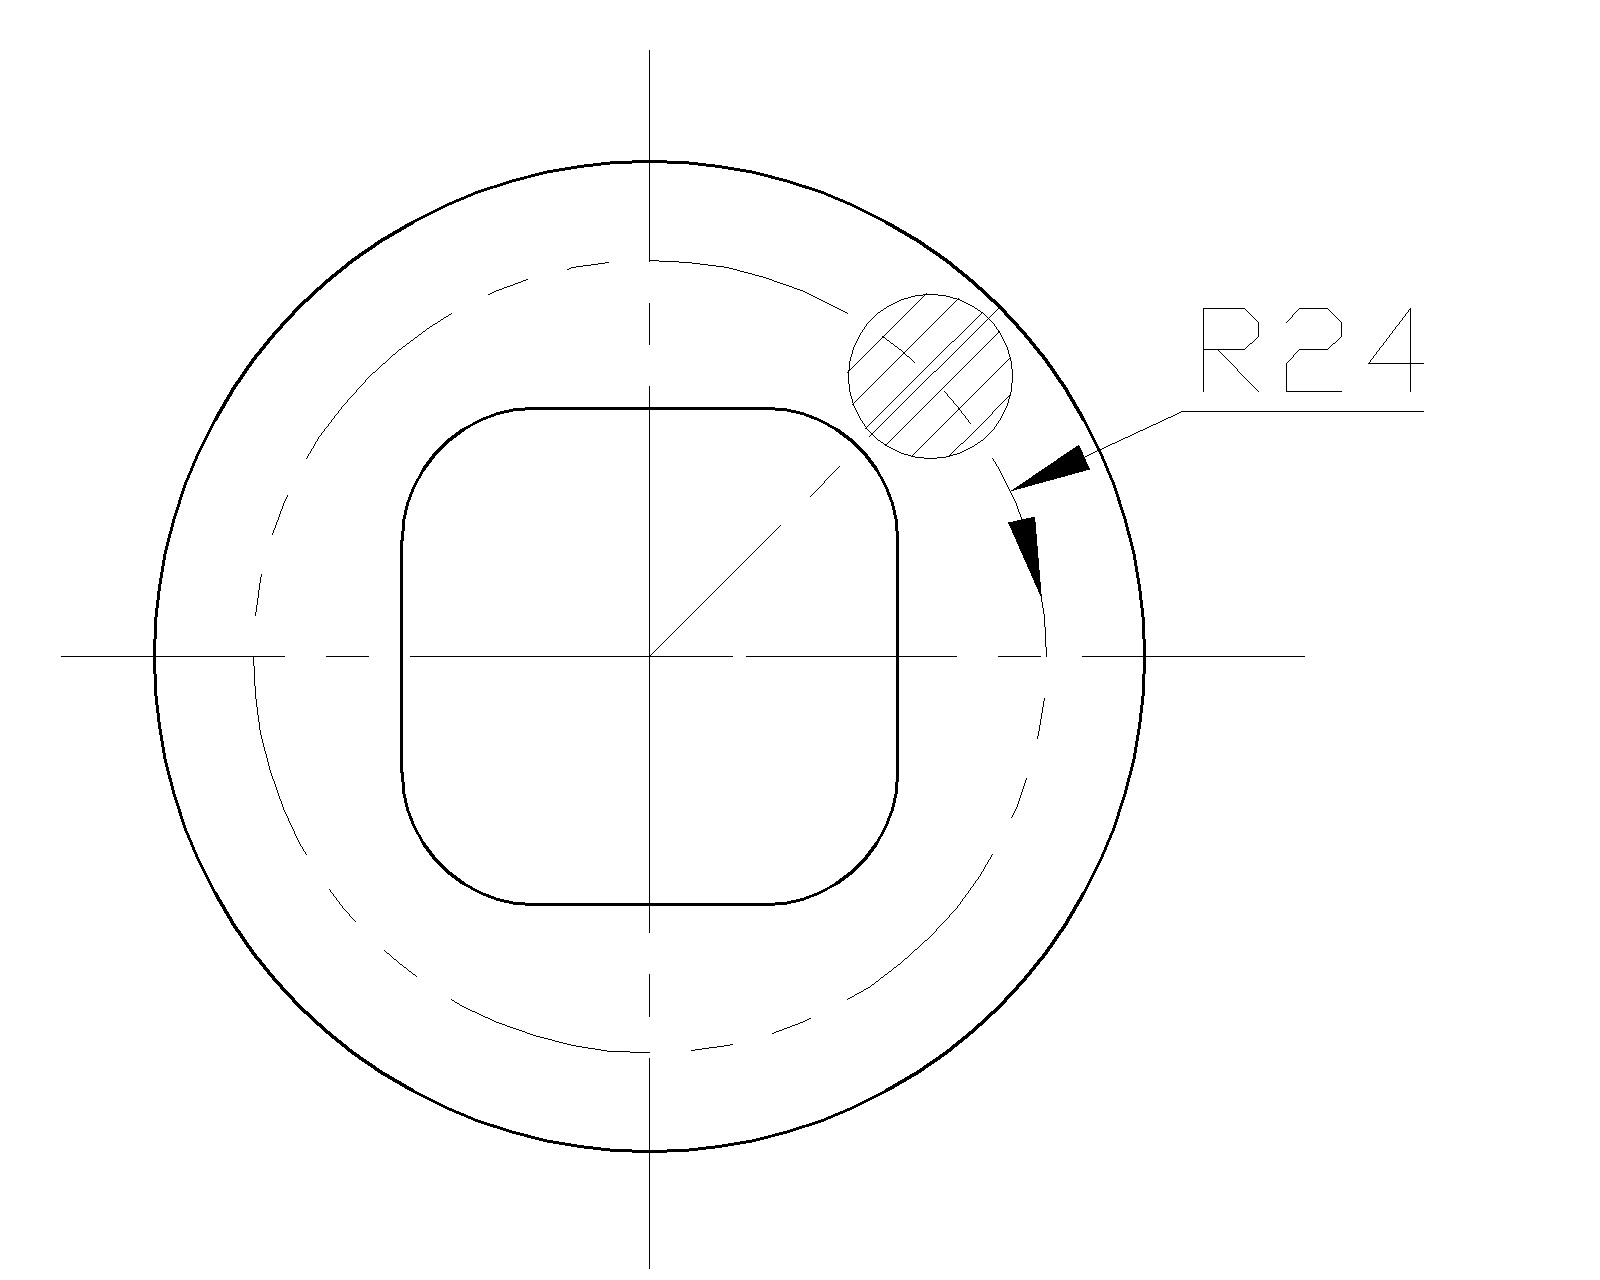
\includegraphics[width=0.6\linewidth,trim=0 0 120  0,clip]{data/image/19-2.jpg}
    \caption{}
    \label{fig:19-2}
\end{figure}

(2)圆形\diameter 60的槽:

路径如图所示:R18、R8

\begin{figure}[h]
    \centering
    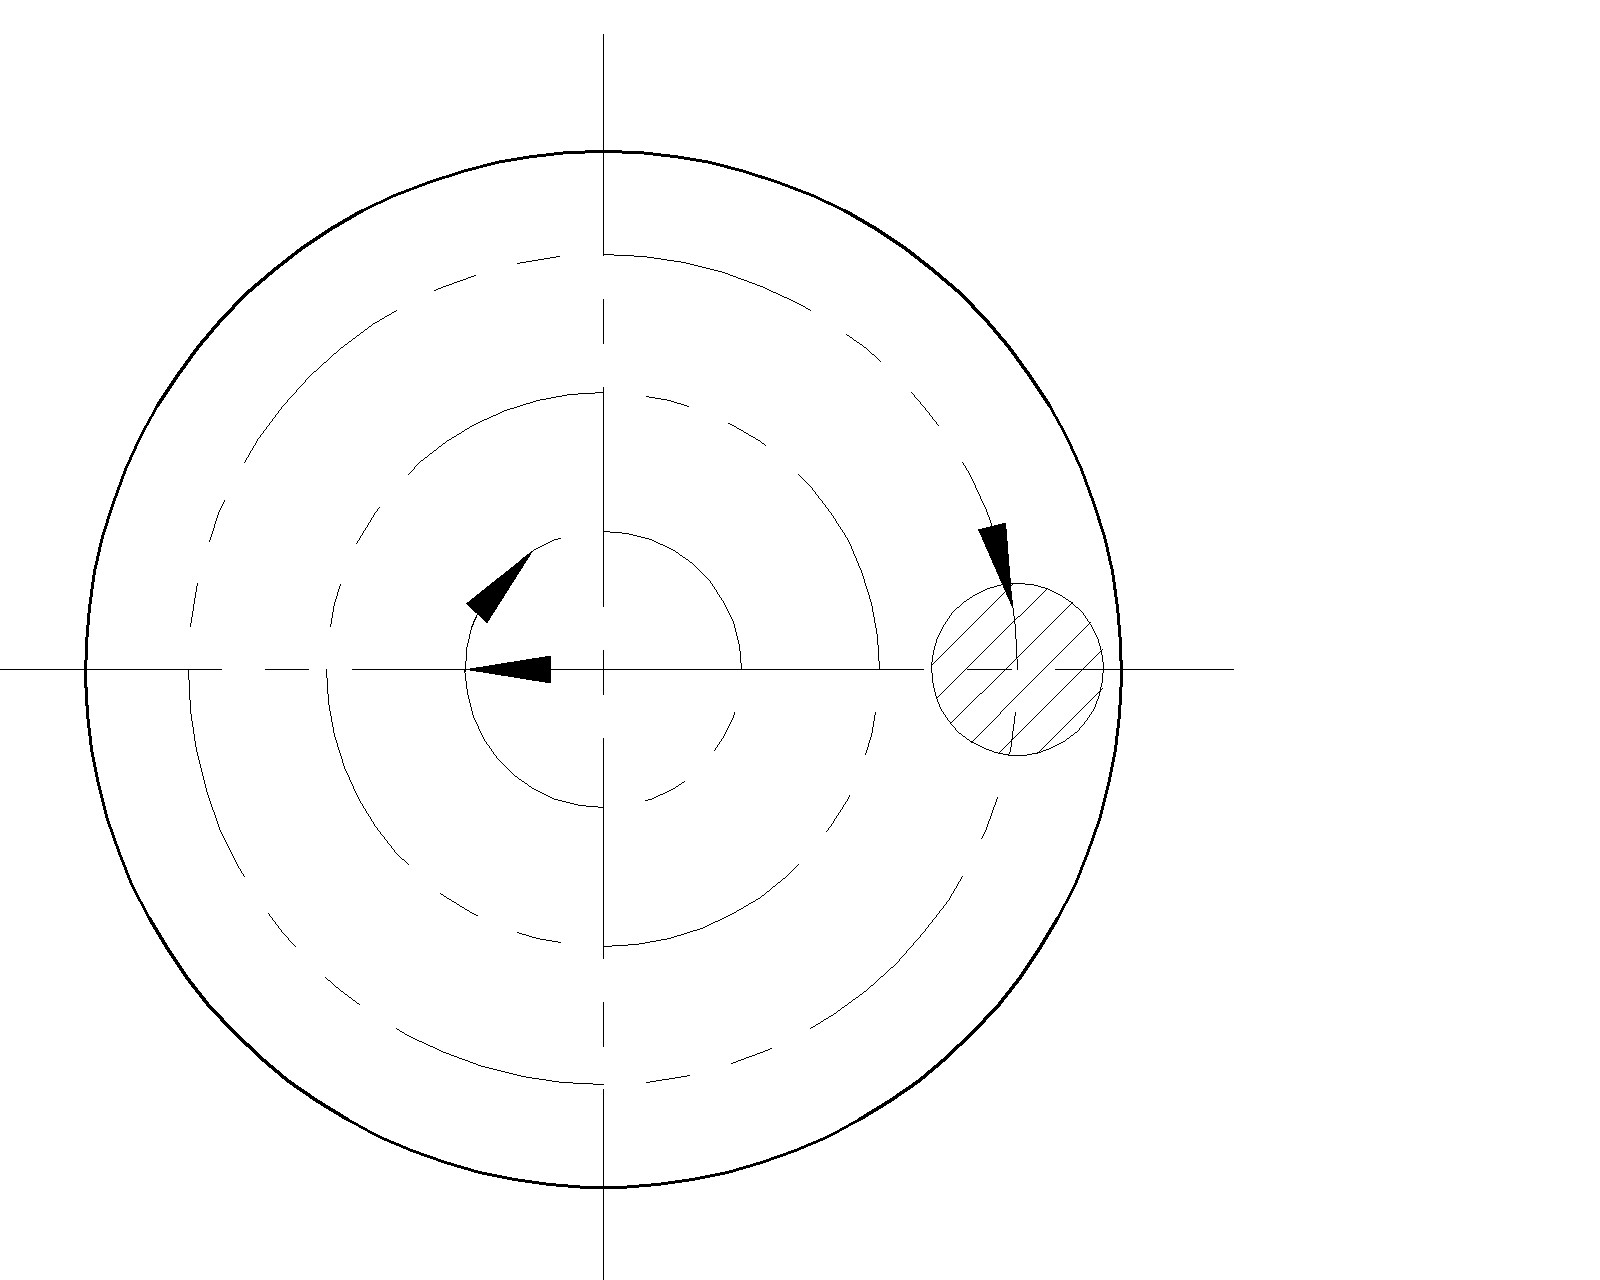
\includegraphics[width=0.6\linewidth,trim=0 0 130  0,clip]{data/image/19-3.jpg}
    \caption{}
    \label{fig:19-3}
\end{figure}

(3)圆形精加工路径

如图所示,要注意不能有干涉,采用顺铣。

\begin{figure}[h]
    \centering
    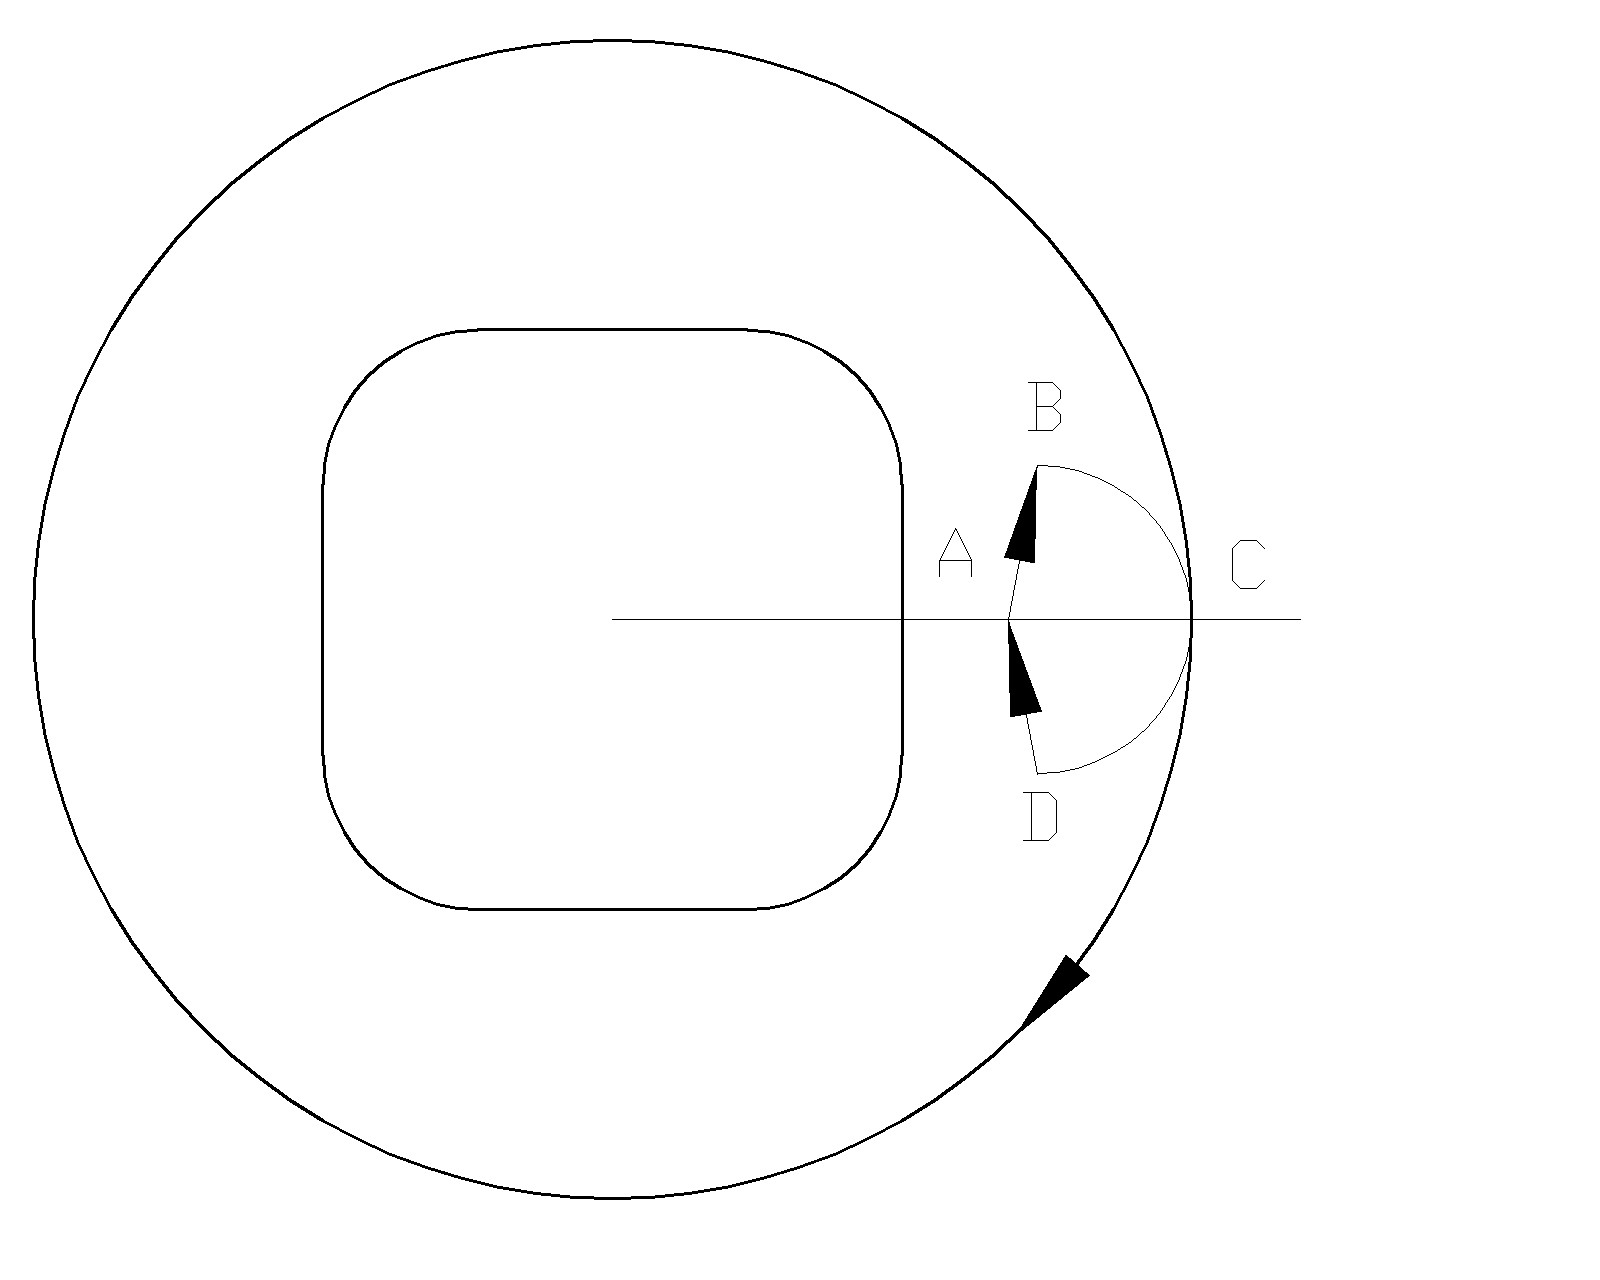
\includegraphics[width=0.6\linewidth,trim=0 0 130  0,clip]{data/image/19-4.jpg}
    \caption{}
    \label{fig:19-4}
    坐标:A(20.5,0)B(22,8)C(30,0)D(22,-8)
\end{figure}


(4)岛屿精加工路径

同上,如图所示:
\begin{figure}[h]
    \centering
    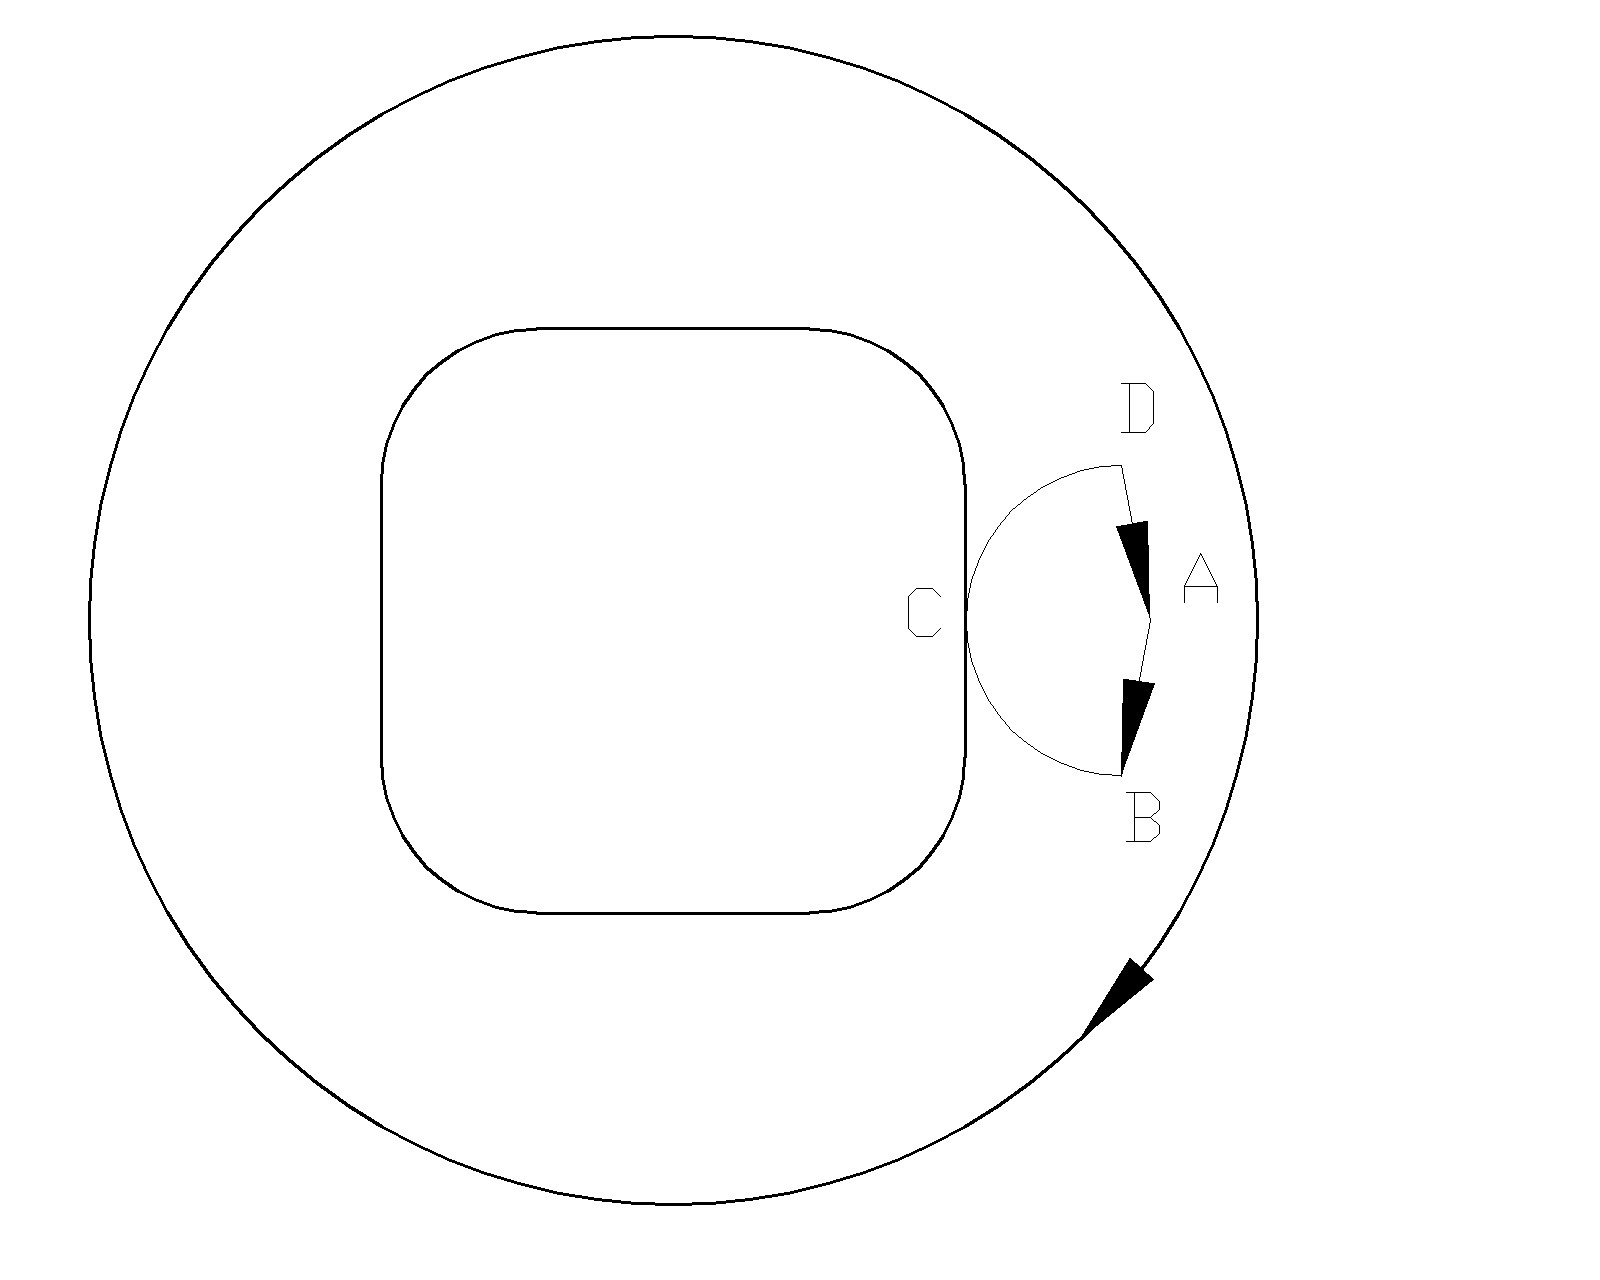
\includegraphics[width=0.6\linewidth,trim=0 0 130  0,clip]{data/image/19-5.jpg}
    \caption{}
    \label{fig:19-5}
    坐标A(24.5,0)B(23,-8)C(15,0)D(23,8)
\end{figure}



(5)方形精加工路径

如图所示:
\begin{figure}[h]
    \centering
    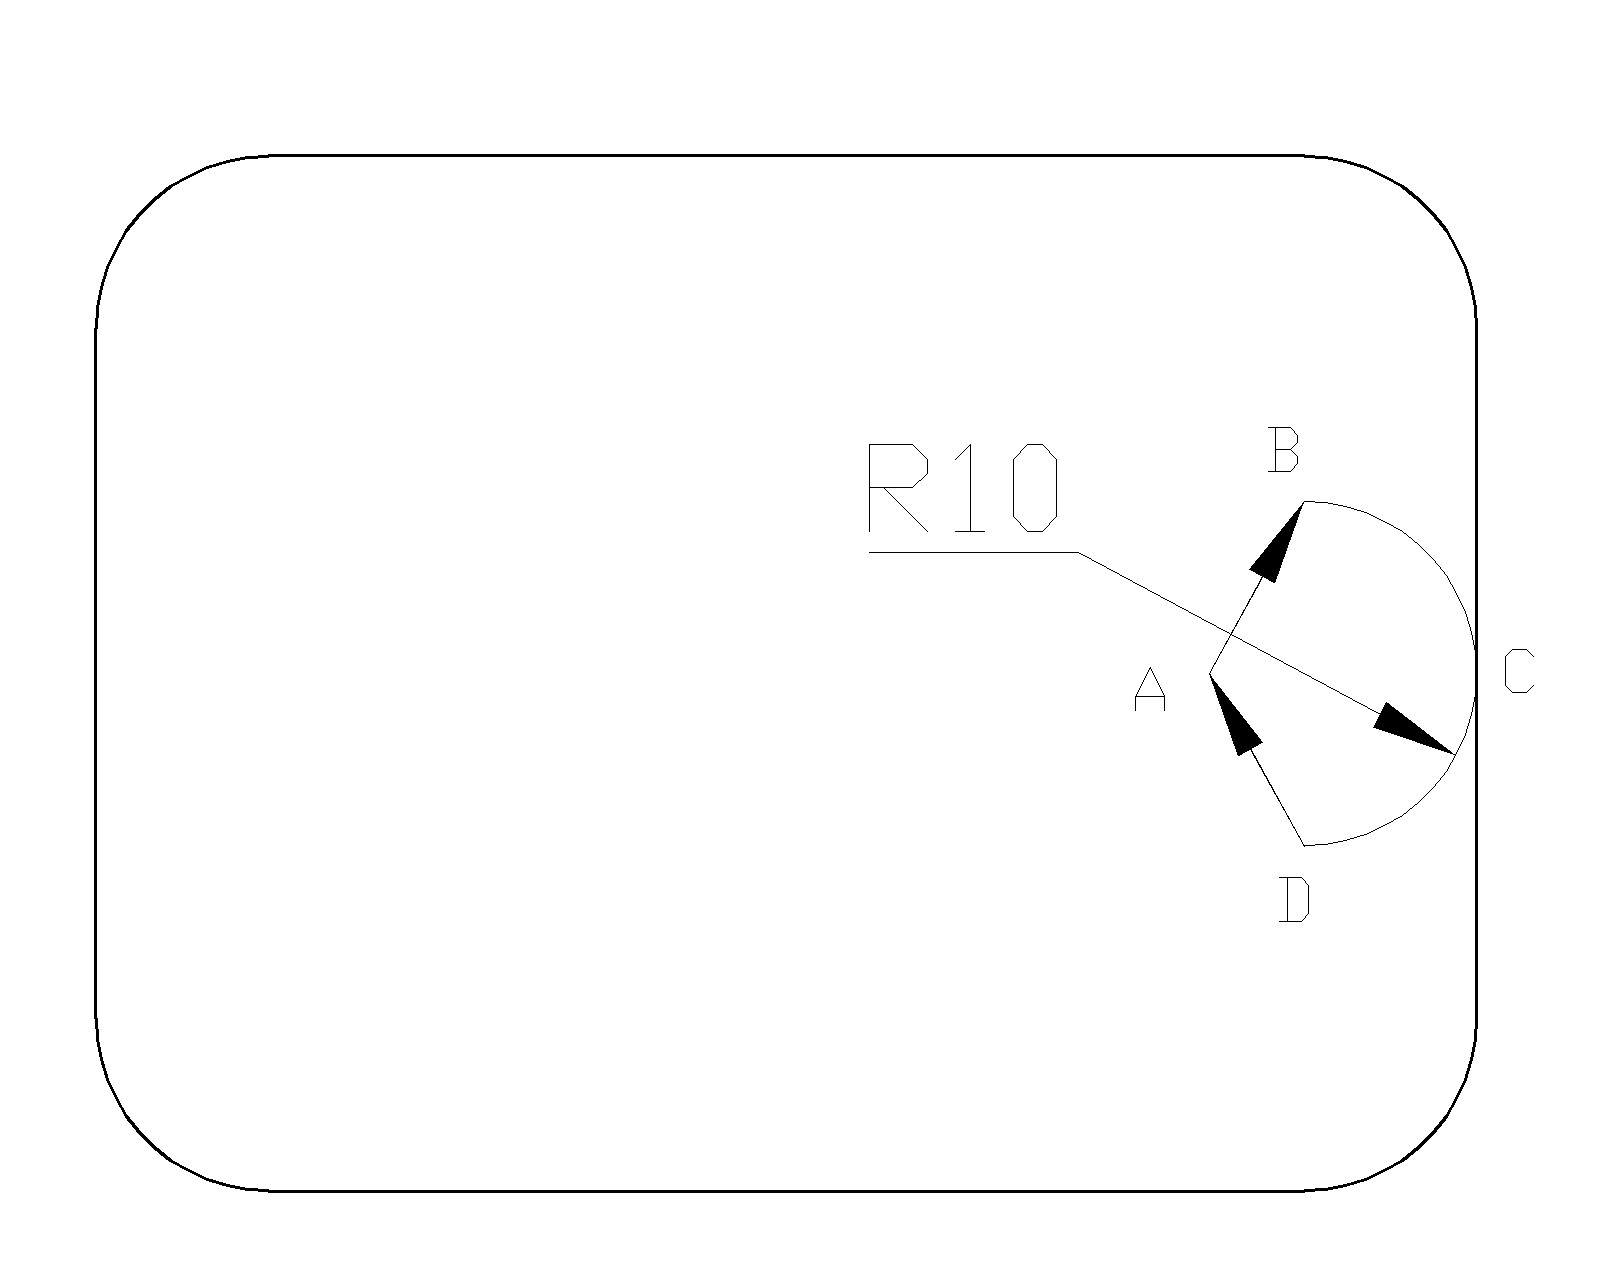
\includegraphics[width=0.6\linewidth,trim=0 0 130  0,clip]{data/image/19-6.jpg}
    \caption{}
    \label{fig:19-6}
    坐标 A(24.5,0)B(30,10)C(40,0)D(30,-10)
\end{figure}

5、Fanuc上的参考程序:
\begin{lstlisting}
O0001;(粗加工主程序)
G54 G17 G40 G49 G90;
M3 S500;
G0 Z30.0;
X24.0 Y0;
Z2.0;
G1 Z0 F100.0;
M98 P20002;    圆形槽
G2 X24.0 Y0 Z-12.0 I-24 J0;   
G2 I-24.0 J0;
G1 X20.5 Y0;    定位到圆形槽A点
D1 M98 P3;     粗加工圆 
G1 X24.5 Y0;    定位到岛屿路径A点
D1 M98 P4;     粗加工岛屿      
G1 Z-4.0;
G1 X27.0 Y0    加工方形槽
Y-17.0
X-27.0
Y17.0
X27.0 
Y0
X24.5 Y0    
D1 M98 P5;   粗加工方形槽
G0 Z30.0;
M5;
M30;
\end{lstlisting}

\begin{lstlisting}
O0002;            粗加工圆形槽
G91 G02 X0 Y0 Z-4.0 I-24.0 J0
G90 G02 I-24.0 J0
G1X-8.0 Y0
G2 I8.0 J0
G1 X-16.0 Y0
G2 I16.0 J0
G1 X20.5 Y0
D1 M98 P3
G1 X24.0 Y0
M99
\end{lstlisting}

\begin{lstlisting}
O0003        圆形槽轮廓子程序
G42 G1 X22.0 Y8.0
G2 X30.0 Y0 R8.0
G2 I-30.0 J0
G2 X22.0 Y-8.0 R8.0
G40 G1 X20.5 Y0
M99
\end{lstlisting}

\begin{lstlisting}
O0004      岛屿轮廓子程序
G42 G1 X23.0 Y-8.0 
G2 X15.0 Y0 R8.0
G1 Y7.0
G3 X7.0 Y15.0 R8.0
G1 X-7.0 
G3 X-15.0 Y7.0 R8.0
G1 Y-7.0 
G3 X-7.0 Y-15.0 R8.0
G1 X7.0 
G3 X15.0 Y-7.0 R8.0
G1 Y0
G2 X23.0 Y8.0 R8.0
G40 G1 X24.5 Y0
M99
\end{lstlisting}

\begin{lstlisting}
O0005        方形槽轮廓子程序
G42 G1 X30.0 Y10.0
G2 X40.0 Y0 R10.0
G1 Y-20.0 
G2 X30.0 Y-30.0 R10.0
G1 X-30.0 
G2 X-40.0 Y-20.0 R10.0
G1 Y20.0 
G2 X-30.0 Y30.0 R10.0
G1 X30.0 
G2 X40.0 Y20.0 R10.0
G1 Y0 
G2 X30.0 Y-10.0 R10.0
G40 G1 X24.5 Y0
M99
\end{lstlisting}

\begin{lstlisting}
O0006       精加工子程序
G54 G17 G40 G49 G90 
M3 S800
G0 Z30.0
X20.5 Y0
Z2.0
G1 Z-12.0 F80
D2 M98 P3
G1 X24.5 Y0
D2 M98 P4
G1 Z-4.0
D2 M98 P5
G0 Z30.0
M99
\end{lstlisting}



\subsection{课堂小结}
\begin{enumerate}[1、]
\item 岛屿型腔加工的下刀方式;
\item 岛屿槽去残料的方式;
\item 用G91螺线下刀及Z向分层;
\item 编写岛屿型腔的程序。
\end{enumerate}

\vfill
\subsection{布置作业}
\begin{enumerate}[1、]
	\item 编写上面的程序。
\end{enumerate}
\vfill
\jxhj{%教学后记
	}
\skrq{%授课日期
	2017年11月21日 4-5节}
\ktmq{%课题名称
	 孔加工概述}
\jxmb{%教学目标,每行前面要加 \item
	\item 掌握孔加工的加工工艺;
	\item 掌握孔加工的六个动作;
	\item 了解用子程序进行孔加工的编程;
	\item 掌握G90/G91在孔加工中的区别。}
\jxzd{%教学重点,每行前面要加 \item
	\item 孔加工的六个动作;
	\item G90/G91在孔加工中的区别。 }
\jxnd{%教学难点,每行前面要加 \item
	\item 用子程序进行孔加工的编程。 }
\jjff{%教学方法
	通过讲述、举例、演示法来说明;}

\makeshouye %制作教案首页

%%%%教学内容
\subsection{组织教学}
\begin{enumerate}[\hspace{2em}1、]
	\item 集中学生注意力;
	\item 清查学生人数;
	\item 维持课堂纪律;
\end{enumerate}

\subsection{复习导入及主要内容}
\begin{enumerate}[1、]
\item 岛屿型腔加工的下刀方式;
\item 岛屿槽去残料的方式;
\item 用G91螺线下刀及Z向分层;
\item 编写岛屿型腔的程序。
\end{enumerate}

\subsection{教学内容及过程}
\subsubsection{孔加工工艺}
1、钻孔

刀具:中心钻(φ3、φ5)

结构形状

钻削深度:

2、钻孔

刀具:直柄麻花钻、锥柄麻花钻、群钻(各种直径)
钻削深度:超出量,0.3倍刀具直径。

3、扩孔

刀具:

4、镗孔:镗刀

5、铰孔加工

刀具:机用绞刀

超出量:刀具值 一般2mm

6、攻丝:

柔性攻丝、刚性攻丝




\subsubsection{孔加工的三个平面及六个动作}
1、三个平面:

初始平面

R点平面

孔底平面

2、六个动作:

XY向快速定位

Z向快速下刀到R点平面

Z向慢速下刀切削

孔底动作

返回到R点平面

快速返回的初始平面

\subsubsection{加工实例}

在数控机床上加工如图所示的零件,是完成孔加工的程序编写。共四个孔,横向间距为80mm,纵向间距为60mm。孔的直径为10H7,有效深度为20mm。

1、刀具的选择:

\diameter 3的中心钻、\diameter9.8的直柄麻花钻、\diameter10H7的机用绞刀。

2、加工工序

3、加工程序


\begin{lstlisting}
02
G54G17G40G90
M3S1200
G1Z30.F2000
X-40.Y30.
M98P21
X40
M98P21
Y-30
M98P21
X-40
M98P21
G1Z30.F2000
M5
M99
\end{lstlisting}
\begin{lstlisting}
O21(G90方式)
G1Z5.0F2000
Z-6.0F80
Z5.0
Z30.F2000
M99
\end{lstlisting}
\begin{lstlisting}
O21(G91方式)
G91G1Z-25.0F2000
Z-11.F80
Z11.
Z25.F2000
G90
M99
\end{lstlisting}

\begin{lstlisting}
O3
G55G17G40G90
M3S500
G1Z30.F2000
X-40.Y30.
M98P31
X40
M98P31
Y-30
M98P31
X-40
M98P31
G1Z30.F2000
M5
M99
\end{lstlisting}

\begin{lstlisting}
O4
G56G17G40G90
M3S500
G1Z30.F2000
X-40.Y30.
M98P41
X40
M98P41
Y-30
M98P41
X-40
M98P41
G1Z30.F2000
M5
M99
……
\end{lstlisting}

\subsubsection{孔加工固定循环}

G99/G98 G90/G91 G81-G89 X Y Z R Q P L


\subsection{课堂小结}
\begin{enumerate}[1、]
\item 孔加工刀具;
\item 孔加工方式;
\item 铣孔与钻孔;
\item 孔加工编程。
\end{enumerate}

\vfill
\subsection{布置作业}
\begin{enumerate}[1、]
	\item 编写上面的程序。
\end{enumerate}
\vfill
\jxhj{%教学后记
	}
\skrq{%授课日期
	2017年11月24日 4-5节}
\ktmq{%课题名称
	 Fanuc上的孔加工指令(一)}
\jxmb{%教学目标,每行前面要加 \item
	\item 掌握孔加工的加工工艺;
	\item 掌握Fanuc上的孔加工指令的选用;
	\item 掌握Fanuc上孔加工指令的使用;
	\item 会进行孔加工程序的编写。}
\jxzd{%教学重点,每行前面要加 \item
	\item Fanuc上孔加工指令的使用;
	\item 进行孔加工程序的编写。 }
\jxnd{%教学难点,每行前面要加 \item
	\item 进行孔加工程序的编写。 }
\jjff{%教学方法
	通过讲述、举例、演示法来说明;}

\makeshouye %制作教案首页

%%%%教学内容
\subsection{组织教学}
\begin{enumerate}[\hspace{2em}1、]
	\item 集中学生注意力;
	\item 清查学生人数;
	\item 维持课堂纪律;
\end{enumerate}

\subsection{复习导入及主要内容}
\begin{enumerate}[1、]
\item 孔加工刀具;
\item 孔加工方式;
\item 铣孔与钻孔;
\item 孔加工编程。
\end{enumerate}

\subsection{教学内容及过程}
\subsubsection{孔加工固定循环指令}
为了简化编程,节省存储空间,把孔加工过程做成固定循环,存储在CNC系统中。Fanuc上的固定循环有G73、G74、G76、G81-G89,其指令格式如下:

\[ 
\left\lbrace 
\begin{array}{c}
G90 \\ G91
\end{array} 
\right\rbrace 
\left\lbrace 
\begin{array}{c}
G99 \\ G98
\end{array} 
\right\rbrace  
 G\_ X\_ Y\_ Z\_ R\_ Q\_ K\_ F\_    \]

说明:

(1)G90/G91:绝对值与增量值,如图11-2,左G90,右G91

(2)G98/G99:返回平面选择

G98返回初始平面

G99返回R点平面

(3)G:孔加工方式

(4)X、Y:孔加工的位置

(5)Z:孔底平面的位置(G91时是R点到孔底的增量值)

(6)R:R点平面的位置(G91时是初始平面到孔
R点平面的增量值,G90时是R点平面Z向绝对坐标)

(7)参数Q:G73、G74深孔中每次Z向进刀量,G76、G87镗孔中的偏移量

(8)参数P:有孔底暂停的暂停时间

(9)参数F:孔加工中的切削速度

(10)参数K、L:固定循环重复次数,结合G91功能更大。

\begin{figure}[h]
	\centering
	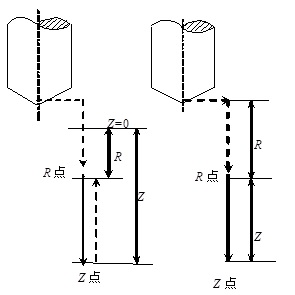
\includegraphics[width=0.7\linewidth]{data/image/21-1}
	\caption{孔加式中的G90与G91}
	\label{fig:21-1}
\end{figure}

注意:孔加工固定循环指令为模态指令,要用G80或01组的指令取消。孔加工参数(重复次数KL除外)也是模态的,在被改变和取消之前一直保持,即使是孔加工方式被改变,也保持。



\subsubsection{孔加工方式其参数}
G81 X\_ Y\_ Z\_ R\_ F\_;用于浅孔,中心孔

G82 X\_ Y\_ Z\_ R\_ P\_ F\_;用于钻孔、锪孔等 

G73 X\_ Y\_ Z\_ R\_ Q\_ F\_;用于深孔(把深孔当作几个浅孔)

G85 X\_ Y\_ Z\_ R\_ F\_;用于铰孔(与G81不同的是慢速提刀)

G84 X\_ Y\_ Z\_ R\_ P\_ F\_;用于右螺纹攻丝

其它:

G74 X\_ Y\_ Z\_ R\_ P\_ F\_;用于左螺纹攻丝

G76 X\_ Y\_ Z\_ R\_ P\_ Q\_ F\_;用于精镗孔

G83 X\_ Y\_ Z\_ R\_ Q\_ F\_;用于深孔、小孔(可排屑)

G86 X\_ Y\_ Z\_ R\_ F\_;用于镗孔(孔底主轴停)

G87 X\_ Y\_ Z\_ R\_ P\_ Q\_ F\_;反向镗孔

G86 X\_ Y\_ Z\_ R\_ F\_;有手动返回的镗孔

G89 X\_ Y\_ Z\_ R\_ P\_ F\_;镗孔(与G85不同的是有孔底暂停)


\subsubsection{加工实例}

加工如\ref{fig:21-2}所示的零件,其中孔的有效深度为30mm。

\begin{figure}
	\centering
	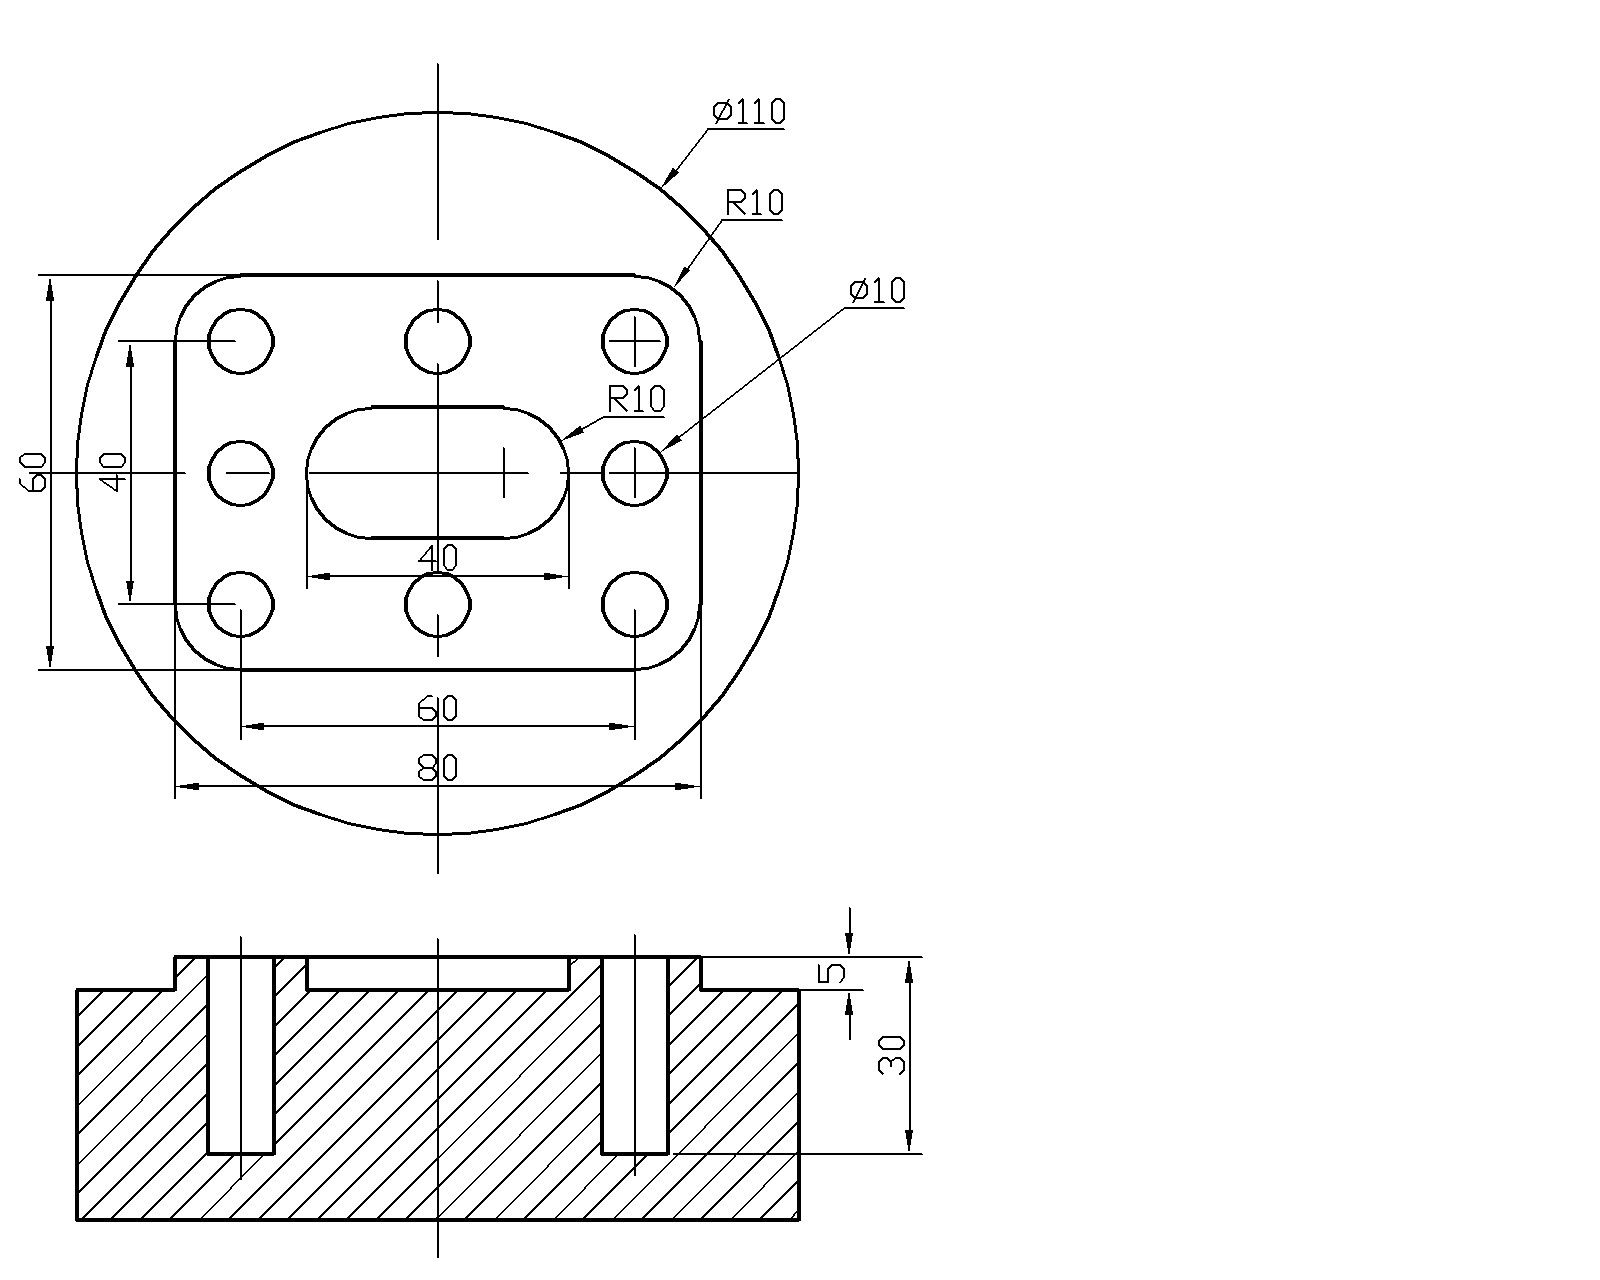
\includegraphics[width=0.5\linewidth,trim=0 0 450  0,clip]{data/image/21-2}
	\caption{孔加工实例}
	\label{fig:21-2}
\end{figure}

1、孔加工方法:钻中心孔、钻孔、铰孔

2、刀具:

$\varnothing $3中心钻(切削刃长10mm,加工深度6-8mm,粗对刀即可)S1200 F120 Z-6.0

$\varnothing $9.8麻花钻 S550 F80.0 Z-35.0 (比32多3mm)

$\varnothing $10机用铰刀 S300 F50 Z-32.0 (比30多2mm)

4、参考程序:
\begin{lstlisting}

O0001;(钻中心孔)
G54 G17 G40 G49 G90;
M3 S1200;
G0 Z30.0;
G99 G81 X-30.0 Y-20.0 Z-6.0 R5.0 F120;
X0
X30.0
Y0
X0
X-30.0
Y20.0
X0
G98 X30.0
M5
M30

\end{lstlisting}

\begin{lstlisting}

O0001;(钻孔)
G55 G17 G40 G49 G90;
M3 S500;
G0 Z30.0;
G99 G83 X-30.0 Y-20.0 Z-6.0 R5.0 Q5.0 F60;
X0
X30.0
Y0
X0
X-30.0
Y20.0
X0
G98 X30.0
M5
M30
\end{lstlisting}


\subsection{课堂小结}
\begin{enumerate}[1、]
\item Fanuc孔加工指令;
\item Fanuc 孔加工应用;
\item Fanuc 孔加工编程;
\item 编程实例。
\end{enumerate}

\vfill
\subsection{布置作业}
\begin{enumerate}[1、]
	\item 综合习题一。
\end{enumerate}
\vfill
\jxhj{%教学后记
	}
\skrq{%授课日期
	2017年11月28日 4-5节}
\ktmq{%课题名称
	 Fanuc上的孔加工指令(二)}
\jxmb{%教学目标,每行前面要加 \item
	\item 掌握孔加工的加工工艺;
	\item 掌握Fanuc上孔加工指令的使用;
	\item 会进行孔加工程序的编写
	\item 掌握孔系的编程。}
\jxzd{%教学重点,每行前面要加 \item
	\item Fanuc上孔加工指令的使用;
	\item 孔系的编程。 }
\jxnd{%教学难点,每行前面要加 \item
	\item 孔系的编程。 }
\jjff{%教学方法
	通过讲述、举例、演示法来说明;}

\makeshouye %制作教案首页

%%%%教学内容
\subsection{组织教学}
\begin{enumerate}[\hspace{2em}1、]
	\item 集中学生注意力;
	\item 清查学生人数;
	\item 维持课堂纪律;
\end{enumerate}

\subsection{复习导入及主要内容}
\begin{enumerate}[1、]
\item Fanuc孔加工指令;
\item Fanuc 孔加工应用;
\item Fanuc 孔加工编程;
\item 编程实例。
\end{enumerate}

\subsection{教学内容及过程}
\subsubsection{一行孔的编程}
加工如图 所示六个孔Ф10,深度为30mm。
\begin{figure}[h]
	\centering
	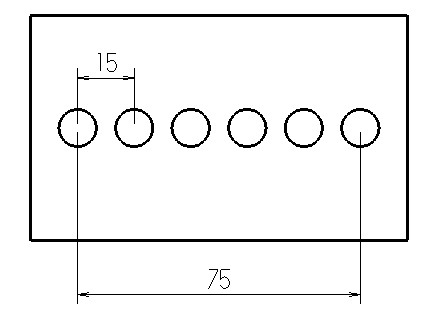
\includegraphics[width=0.7\linewidth]{data/image/22-1}
	\caption{线性均布孔实例}
	\label{fig:22-1}
\end{figure}

分析:

图中六个孔分布在同一条线上,且间距均为15mm,为了减少程序量,可以使用重复次数指令L\_\_编程。工件坐标系设置于工件上表面中心处。
加工程序如下:
\begin{lstlisting}
O21
G54G17G40G49G80
G01Z100F2000
M03S400
Z20                      
G00X-52.5Y0              定位于最左侧孔的左侧
G99G73Z-30R5Q6F80L0      定义孔加工参数的方式及相关参数
G91X15L6                 从左往右依次加工六个孔
G80
M05
M30
\end{lstlisting}

\subsubsection{一列孔的编程}
\begin{lstlisting}
O21
G54G17G40G49G80
G01Z100F2000
M03S400
Z20                      
G00X-52.5Y0              定位于最左侧孔的左侧
G99G73Z-30R5Q6F80L0      定义孔加工参数的方式及相关参数
G91Y-15L6                 从左往右依次加工六个孔
G80
M05
M30
\end{lstlisting}

\subsubsection{斜线孔系的编程}
\begin{lstlisting}
O21
G54G17G40G49G80
G01Z100F2000
M03S400
Z20                      
G00X-52.5Y0              定位于最左侧孔的左侧
G99G73Z-30R5Q6F80L0      定义孔加工参数的方式及相关参数
G91Y-15X10L6                 从左往右依次加工六个孔
G80
M05
M30
\end{lstlisting}

\subsubsection{多行孔系的编程}
\begin{lstlisting}
O21
G54G17G40G49G80
G01Z100F2000
M03S400
Z20                      
G00X-52.5Y0              定位于最左侧孔的左侧
M98 P10 L10                从左往右依次加工六个孔
G80
M05
M30

O10
G99G73Z-30R5Q6F80L0      定义孔加工参数的方式及相关参数
G91X15L6 
G1X-15Y10
M99
\end{lstlisting}


\subsection{课堂小结}
\begin{enumerate}[1、]
\item 一行孔的编程;
\item 一列孔的编程;
\item 斜线孔系的编程;
\item 多行孔系的编程。
\end{enumerate}

\vfill
\subsection{布置作业}
\begin{enumerate}[1、]
	\item 综合习题一。
\end{enumerate}
\vfill
\jxhj{%教学后记
	}
\skrq{%授课日期
	2017年11月30日 4-5节}
\ktmq{%课题名称
	 Siemens上的孔加工指令}
\jxmb{%教学目标,每行前面要加 \item
	\item 掌握孔加工的加工工艺;
	\item 掌握Siemens上的孔加工指令的选用;
	\item 掌握Siemens上孔加工指令的使用;
	\item 会进行孔加工程序的编写。}
\jxzd{%教学重点,每行前面要加 \item
	\item Siemens上孔加工指令的使用;
	\item 进行孔加工程序的编写。 }
\jxnd{%教学难点,每行前面要加 \item
	\item 进行孔加工程序的编写。 }
\jjff{%教学方法
	通过讲述、举例、演示法来说明;}

\makeshouye %制作教案首页

%%%%教学内容
\subsection{组织教学}
\begin{enumerate}[\hspace{2em}1、]
	\item 集中学生注意力;
	\item 清查学生人数;
	\item 维持课堂纪律;
\end{enumerate}

\subsection{复习导入及主要内容}
\begin{enumerate}[1、]
\item 一行孔的编程;
\item 一列孔的编程;
\item 斜线孔系的编程;
\item 多行孔系的编程。
\end{enumerate}

\subsection{教学内容及过程}
\subsubsection{SIEMENS 孔加工循环概述}
SIEMENS上的固定循环就是一些工艺子程序,分为钻削循环
、钻孔样式循环和铣削循环。

名称如下:

\begin{enumerate}
	\item 钻孔循环 
\begin{itemize}
\item 	CYCLE81    钻孔,中心钻孔 
\item CYCLE82    中心钻孔 
\item CYCLE83    深度钻孔 
\item CYCLE84    刚性攻丝 
\item CYCLE840   带补偿卡盘攻丝 
\item CYCLE85    铰孔1(镗孔1) 
\item CYCLE86    镗孔(镗孔2) 
\item CYCLE87    铰孔2(镗孔3) 
\item CYCLE88    镗孔时可以停止1(镗孔4) 
\item CYCLE89    镗孔时可以停止2(镗孔5)

\end{itemize}
\vspace{10pt}

\item 钻孔样式循环  
\begin{itemize}
	\item HOLES1    加工一排孔 
\item HOLES2    加工一圈孔  
\end{itemize}
\vspace{10pt}
\item 铣削循环 
\begin{itemize}
	\item CYCLE71    端面铣削 
\item CYCLE72    轮廓铣削 
\item CYCLE76    矩形过渡铣削 
\item CYCLE77    圆弧过渡铣削 
\item LONGHOLE   槽 
\item SLOT1    圆上切槽 
\item SLOT2    圆周切槽 
\item POCKET3    矩形凹槽 
\item POCKET4    圆形凹槽 
\item CYCLE90    螺纹铣削
\end{itemize}

\end{enumerate}
\vspace{10pt}
编程器中图形循环支持,根据图形直观的输入参数。

\subsubsection{孔加工固定循环指令}

钻孔,中心孔-CYCLE81

格式:CYCLE81(RTP,RFP,SDIS,DP,DPR)

RTP 后退平面(绝对) 

RFP 参考平面(绝对) 

SDIS 安全间隙(无符号输入) 

DP 最后钻孔深度(绝对) 

DPR相当于参考平面的最后钻孔深度(无符号输入)

\begin{figure}[h]
	\centering
	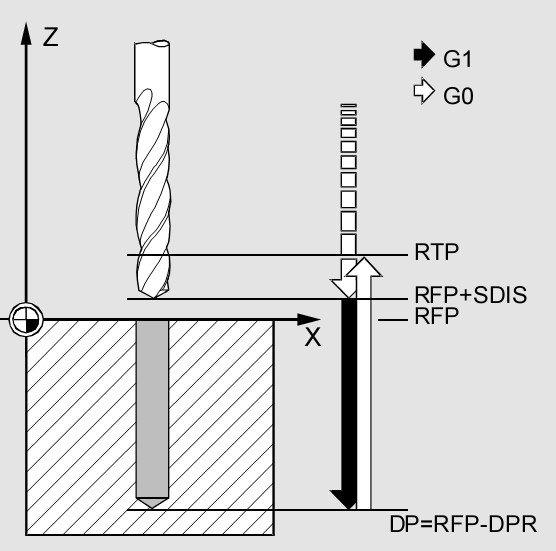
\includegraphics[width=0.7\linewidth]{data/image/23-1}
	\caption{动作顺序}
	\label{fig:23-1}
\end{figure}

如果一个值同时输入给DP和DPR,最后钻孔深度则来自DPR。

CYCLE82(RTP,RFP,SDIS,DP,DPR,DTB)

RTP Real 后退平面(绝对)

RFP Real 参考平面(绝对) 

SDIS Real 安全间隙(无符号输入) 

DP Real 最后钻孔深度(绝对)
 
DPR Real 相当于参考平面的最后钻孔深度(无符号输入) 

DTB Real 最后钻孔深度时的停顿时间(断屑)

\begin{figure}[h]
	\centering
	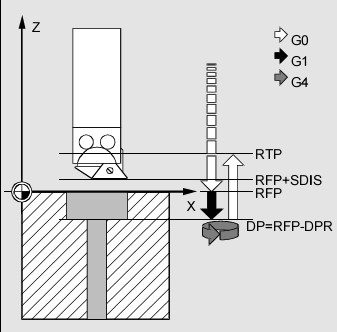
\includegraphics[width=0.7\linewidth]{data/image/23-2}
	\caption{动作顺序}
	\label{fig:23-2}
\end{figure}

CYCLE85(RTP,RFP,SDIS,DP,DPR,DTB,FFR,RFF)

RTP Real 退回平面(绝对值) 

RFP Real 参考平面(绝对值) 

SDIS Real 安全间隙(无符号输入) 

DP Real 最后钻孔深度(绝对值) 

DPR Real 相对于参考平面的最后钻孔深度(无符号输入) 

DTB Real 最后钻孔深度时的停顿时间(断屑) 

FFR Real 进给率 

RFF Real 退回进给率

\begin{figure}[h]
	\centering
	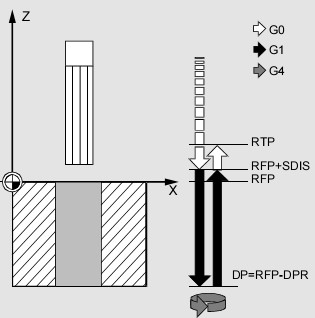
\includegraphics[width=0.7\linewidth]{data/image/23-3}
	\caption{动作顺序}
	\label{fig:23-3}
\end{figure}

注意: 循环调用前设定好率,主轴转速和和转向,
循环调用前必须使刀具到达钻孔位置,
之前的G功能,之后还有效。

\subsubsection{模态调用}

在有MCALL指令的程序段中调用子程序,如果其后的程序段中含有轨迹运行,则子程序会自动调用。该调用一直有效,直到调用下一个程序段。 

用MCALL指令模态调用子程序的程序段以及模态调用结束指令均需要一个独立的程序段。

比如可以使用MCALL指令来方便地加工各种排列形状的孔。

N10 MCALL CYCLE82(…)      ;钻削循环82 

N20 HOLES1(…)    ;行孔循环,在每次到达孔位置之
后,使用传送参数执行CYCLE82(…)循环 

N30 MCALL    ;结束CYCLE82(…)的模态调用

\subsubsection{加工实例}

加工如\ref{fig:21-2}所示的零件,其中孔的有效深度为30mm。

\begin{figure}
	\centering
	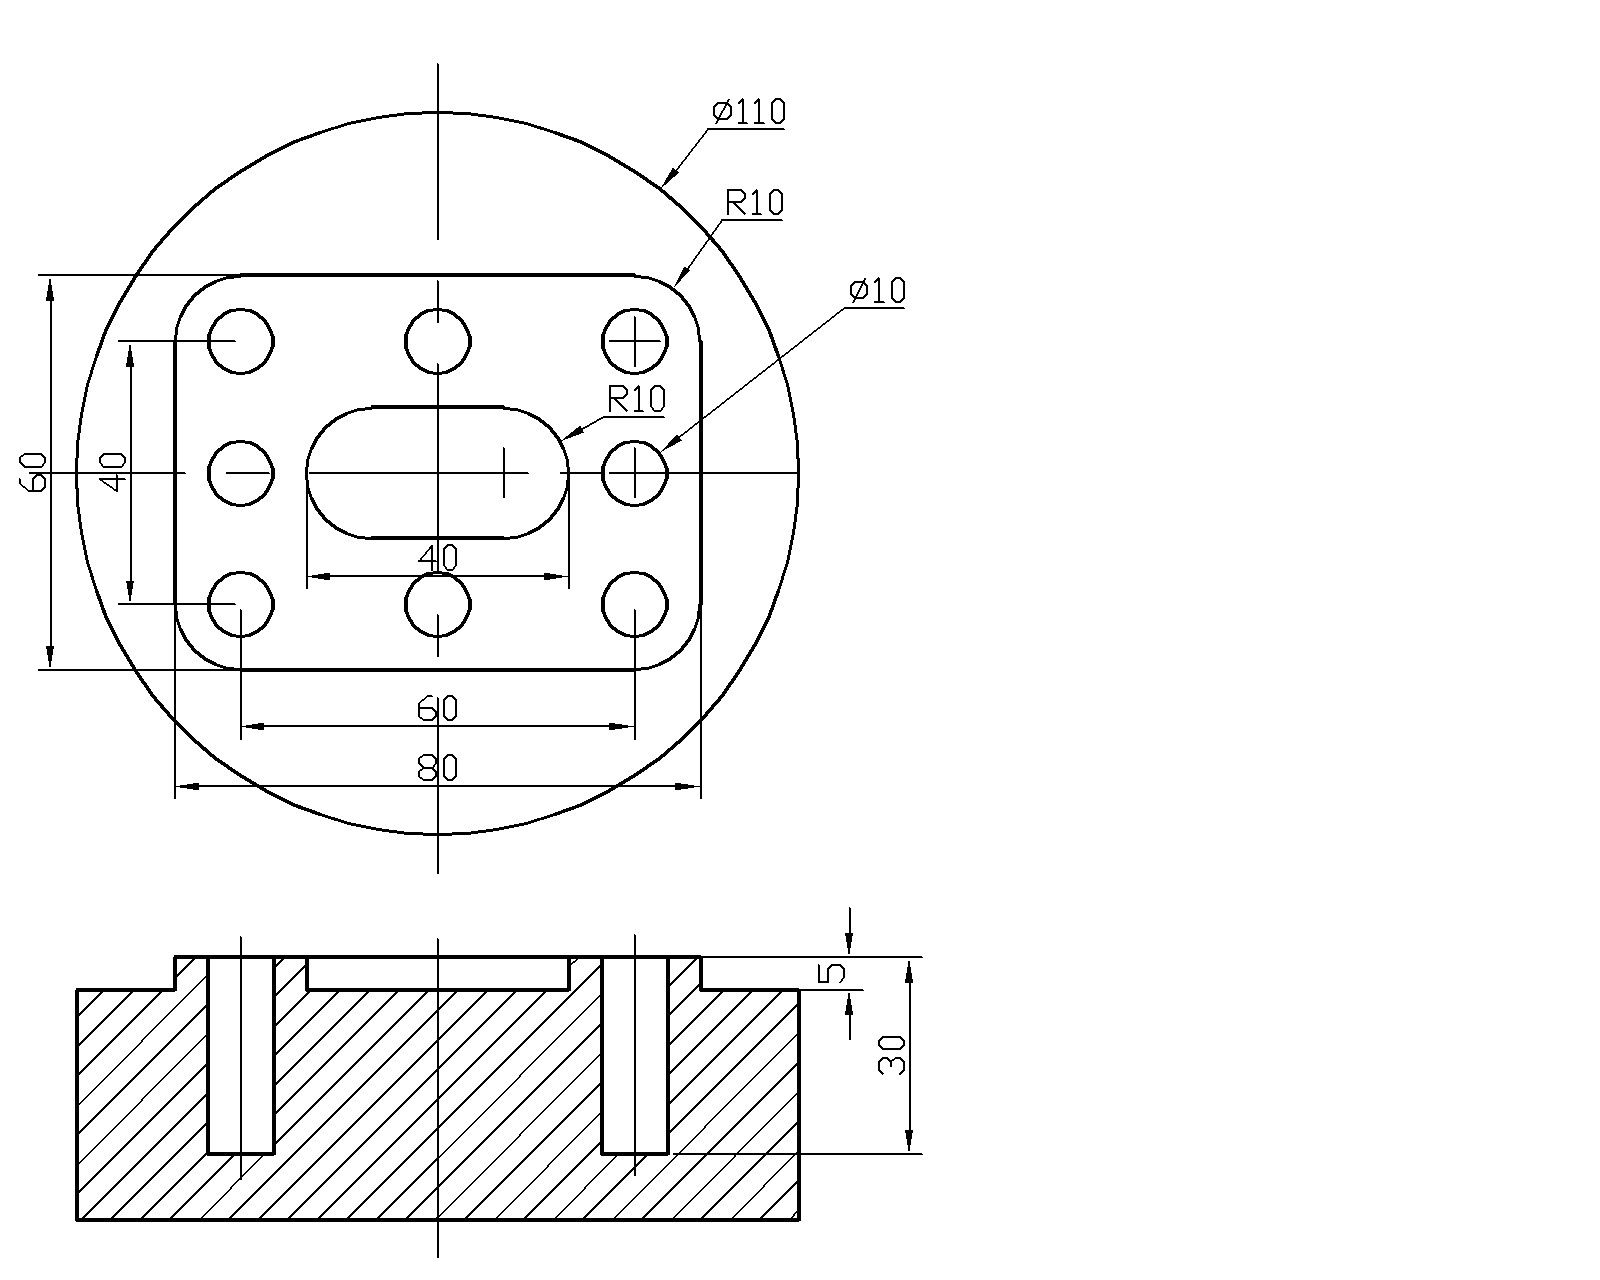
\includegraphics[width=0.5\linewidth,trim=0 0 450  0,clip]{data/image/21-2}
	\caption{孔加工实例}
	\label{fig:21-2}
\end{figure}

1、孔加工方法:钻中心孔、钻孔、铰孔

2、刀具:

$\varnothing $ 3中心钻(切削刃长10mm,加工深度6-8mm,粗对刀即可)S1200 F120 Z-6.0

$\varnothing $ 9.8麻花钻 S550 F80.0 Z-35.0 (比32多3mm)

$\varnothing $ 10机用铰刀 S300 F50 Z-32.0 (比30多2mm)

4、参考程序:
\begin{lstlisting}
GX01
G54G17G40G90
M3S1000
G1Z30.F2000
F60
MCALL CYCLE81(30,0,3,-8,8)
G0X-30Y20
X0
Y20
X30
Y0
Y-20
X0
X-30
Y0
MCALL
M5
M2
\end{lstlisting}



\subsection{课堂小结}
\begin{enumerate}[1、]
\item Siemens孔加工循环概述;
\item 孔加工固定循环指令;
\item 模态调用;
\item 加工实例。
\end{enumerate}

\vfill
\subsection{布置作业}
\begin{enumerate}[1、]
	\item 综合习题一。
\end{enumerate}
\vfill
\jxhj{%教学后记
	}
\skrq{%授课日期
	2017年12月5日 4-5节}
\ktmq{%课题名称
	 长度补偿概述}
\jxmb{%教学目标,每行前面要加 \item
	\item 掌握G43、G44、G49指令的格式;
	\item 掌握刀具相对长度的测量;
	\item 掌握刀具长度补偿的编程思路。
}
\jxzd{%教学重点,每行前面要加 \item
	\item 掌握G43、G44、G49指令的格式;
	\item 掌握刀具长度补偿的编程思路。 }
\jxnd{%教学难点,每行前面要加 \item
	\item 掌握刀具相对长度的测量。 }
\jjff{%教学方法
	通过讲述、举例、演示法来说明;}

\makeshouye %制作教案首页

%%%%教学内容
\subsection{组织教学}
\begin{enumerate}[\hspace{2em}1、]
	\item 集中学生注意力;
	\item 清查学生人数;
	\item 维持课堂纪律;
\end{enumerate}

\subsection{复习导入及主要内容}
\begin{enumerate}[1、]
\item Siemens孔加工循环概述;
\item 孔加工固定循环指令;
\item 模态调用;
\item 加工实例。
\end{enumerate}

\subsection{教学内容及过程}

加工中心或铣床在加工中都要使用很多刀具,但每把刀具的长度都不同,这样在加工时要进行长度补偿后,才能每把刀加工出来的深度都正确。

\subsubsection{补偿长度}
具安装在刀柄上,如图\ref{fig:24-1}所示,刀具安装的深度不同其补偿长度也就不同,故长度包括刀具和刀柄上的两个部分,一般就取刀具安装到主轴上后,刀具参考点到刀位点的距离,补偿长度一般就用刀具之间的相对长度。

绝对长度:刀具安装在刀柄上的整体长度,一般取刀具参考点到刀位点的距离。只用G43,无基准刀。

相对长度:待测刀相对于基准刀的长度,有正有负。

\begin{figure}[h]
	\centering
	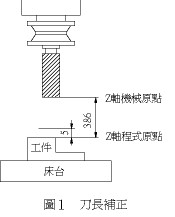
\includegraphics[width=0.7\linewidth]{data/image/24-1}
	\caption{补偿长度}
	\label{fig:24-1}
\end{figure}

\subsubsection{长度补偿方向的确定}

刀具长度补偿有G43、G44、G49三个指令:

G43为刀具长度的正补偿

G44为刀具长度的负补偿

G49为刀具取消刀具长度补偿

有两种用法:

(1)只用G43和G49指令,补偿值取正负

(2)补偿值只取正值,正负由G43及G44确定

如图\ref{fig:24-2}所示:(T1般预留)

T2设为基准刀具,相对长度为0

T3比T2短,应向Z负方向补偿,即用G44负补偿5mm;

T4比T2长,应向Z正方向补偿,即用G43正补偿7mm;

T2相对长度为0,用G49取消长度补偿。

其中,T3也可用G43正补偿-5mm。

即,只用G43和G49指令时,补偿长度的计算如下:

补偿长度=待测刀长-基准刀长 

注意:有正有负;

\begin{figure}[h]
	\centering
	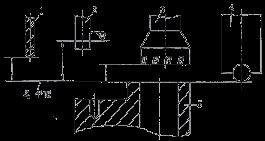
\includegraphics[width=0.7\linewidth]{data/image/24-2}
	\caption{补偿长度}
	\label{fig:24-2}
\end{figure}
\subsubsection{长度补偿值的确定}

绝对长度:刀具长度测量仪

相对长度:刀具长度测量仪

机内对刀测量法

机内自动对刀法(用G31及G10来实现)

1、用刀具长度测量仪



2、用自动对刀仪结合G31自动测量

略

3、手动的用机内对刀法测量:

A安装基准刀,将其移动到一个确定的位置,将Z向的相对坐标设置为0

B、安装待测刀,将其移动到相同的位置,记录Z向的相对坐标,这个值就是长度补偿值,有正有负。

如图\ref{fig:24-3}所示:
\begin{figure}[h]
	\centering
	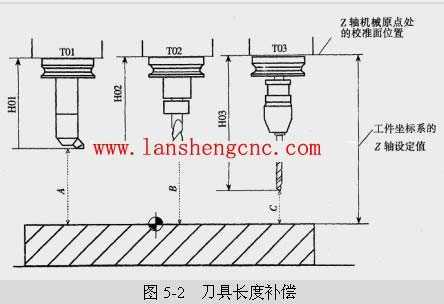
\includegraphics[width=0.7\linewidth]{data/image/24-3}
	\caption{补偿长度}
	\label{fig:24-3}
\end{figure}

\subsubsection{换刀}
数控铣床上换刀时,可在程序中加入:
\begin{lstlisting}:
G0 Z50.0
M05;
M00;
:
\end{lstlisting}
加工中心上换刀:
\begin{lstlisting}:
:
G28G91Z0;第一次换刀前要回零。

G90;
Tn M6;
G90 G1 Z100.0 G43 Hn F__;
M3 S500;
:
G0 Z____;
G49 G1 Z100.0;
M5
G0Z30.0
Tn M6
G90G43G1X
M03 S500;
\end{lstlisting}



\subsection{课堂小结}
\begin{enumerate}[1、]
\item 长度补偿概述;
\item 长度补偿方向的确定;
\item 长度补偿值的确定;
\item 换刀指令。
\end{enumerate}

\vfill
\subsection{布置作业}
\begin{enumerate}[1、]
	\item 综合习题一。
\end{enumerate}
\vfill
\jxhj{%教学后记
	}
\skrq{%授课日期
	2017年12月7日 4-5节}
\ktmq{%课题名称
	 长度补偿应用}
\jxmb{%教学目标,每行前面要加 \item
	\item 掌握Fanuc上的长度补偿指令;
	\item 掌握Fanuc长度补偿的执行过程;
	\item 掌握Fanuc长度补偿的编程;
	\item 会进行各种长度补偿的使用。}
\jxzd{%教学重点,每行前面要加 \item
	\item Fanuc长度补偿的执行过程;
	\item 长度补偿的编程。 }
\jxnd{%教学难点,每行前面要加 \item
	\item 进行各种长度补偿的使用。 }
\jjff{%教学方法
	通过讲述、举例、演示法来说明;}

\makeshouye %制作教案首页

%%%%教学内容
\subsection{组织教学}
\begin{enumerate}[\hspace{2em}1、]
	\item 集中学生注意力;
	\item 清查学生人数;
	\item 维持课堂纪律;
\end{enumerate}

\subsection{复习导入及主要内容}
\begin{enumerate}[1、]
\item 长度补偿概述;
\item 长度补偿方向的确定;
\item 长度补偿值的确定;
\item 换刀指令。
\end{enumerate}

\subsection{教学内容及过程}
\subsubsection{长度补偿的执行过程}
	
	过程一:
	
	补偿时,先进行补偿,后进行定位
	
	取消时,先取消补偿,后进行定位
	
	注意安全问题:
	
	程序启动前,要求刀具工件表面有足够的补偿空间。
	
	取消之前,先提刀,保证有足够的取消空间
	
	过程二:
	
	补偿时,补偿与定位计算,直接一次移动到位。
	
	取消时,取消与定位计算,直接一次移动到位。
	
	这种方法使用安全
	
\subsubsection{安全使用长度补偿}
	
	1、程序启动前,要求刀具到工件表面的距离大于最大的刀具长度补偿。
	
	2、程序中取消刀补,要求先提刀到一个较高的位置,在取消。
	
	即使用及取消刀具长度补偿要有足够的空间。
	
	3、编程要求
	
	G43G1Z150.H1 (Z150大于最大的刀具半径补偿)
	
	……
	
	G1Z100.F2000 (提刀到一个较高的位置)
	
	G49G1Z150.
	
	……
	
\subsubsection{三种补偿值的比较}
	
	1、相对长度:
	
	容易理解,但基准刀攷变时,所有的补偿要重新设置,
	
	补偿值有正有负,为正时不安全。
	
	用基准刀对刀,对刀方便。
	
	2、绝对长度:
	
	使用刀具的绝对长度,补偿值不变,补偿值始终为正,使用不太安全
	。对刀要考虑刀具的长度,
	
	3、空间移动距离
	
	即在绝对长度的基础上,把补偿值变换为负值。
	方法,把坐标系往上提高一个距离,刀具向负方向补偿一个距离。
	
\subsubsection{编程实例}
	
	在数控机床上加工如图所示的零件,试按加工中心机床进行零件的工艺分析及程序的编写。
	
	综合加工,如图9-5所示。毛坯:80*80*45。要求:
	
	(1)面铣:保证厚度为44 
	     
	(2)轮廓铣:粗/精加工(内凸台高15mm、外凸台高15mm)    
	  
	(3)型腔铣:粗/精加工(矩形深5mm,圆形深10mm) 
	    
	(4)孔加工:$\varnothing $8H7(深25mm)
	
	刀具:面铣$\varnothing $80         粗加工$\varnothing $16、$\varnothing $12   
	   
	精加工$\varnothing $8        孔$\varnothing $5、$\varnothing $7.8   $\varnothing $8H7
	
	\begin{figure}[h]
		\centering
		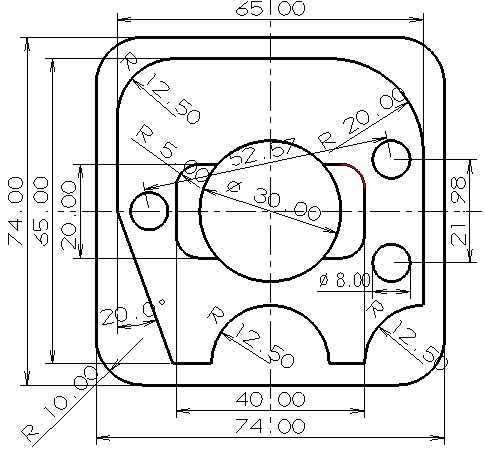
\includegraphics[width=0.7\linewidth]{data/image/25-1}
		\caption{编程实例}
		\label{fig:25-1}
	\end{figure}
	
	1、图形分析
	
	2、坐标系及装夹
	
	3、刀具及工序标
	
	A 铣上表面  $\varnothing$80面铣刀 T1H1 S400 F200 
	
	B 粗铣外形  $\varnothing$16立铣刀 T2H2 S500 F200 D1=8.5
	
	C 粗铣槽    $\varnothing$12 立铣刀 T3H3 S500 F200 D2=6.5
	
	D 精加工    $\varnothing$8立铣刀  T4H4  S800 F100 D3=6.2
	
	E 钻中心空  $\varnothing$3中心钻   T5H5 S1000 F60
	
	F 钻孔     $\varnothing$7.8麻花钻 T6H6 S500  F80
	
	H 铰孔      $\varnothing$8H7机用铰刀  T7H7 S300 F30
	
	
	4、参考程序
	\begin{lstlisting}
	O1
	G28G91ZO
	T1M6
	M98P2 (铣平面)
	G28G91Z0
	T2M6
	M98P3 (铣方)
	M98P4  (铣外形)
	G28G91Z0
	T3M6
	M98P5  (铣槽)
\end{lstlisting}

\subsection{课堂小结}
\begin{enumerate}[1、]
\item Fanuc长度补偿的执行过程;
\item 安全使用长度补偿;
\item 三种补偿值的比较;
\item 编程实例。
\end{enumerate}

\vfill
\subsection{布置作业}
\begin{enumerate}[1、]
	\item 综合习题一。
\end{enumerate}
\vfill
\jxhj{%教学后记
	}
\skrq{%授课日期
	2017年12月12日 4-5节}
\ktmq{%课题名称
	 Siemens上的长度补偿}
\jxmb{%教学目标,每行前面要加 \item
	\item 掌握Siemens上的换刀指令;
\item 掌握Siemens上的长度补偿;
\item 掌握Siemens长度补偿编程。}
\jxzd{%教学重点,每行前面要加 \item
	\item Siemens上的长度补偿;
	\item 掌握加工中心编程。 }
\jxnd{%教学难点,每行前面要加 \item
	\item Siemens上的长度补偿。 }
\jjff{%教学方法
	通过讲述、举例、演示法来说明;}

\makeshouye %制作教案首页

%%%%教学内容
\subsection{组织教学}
\begin{enumerate}[\hspace{2em}1、]
\item 集中学生注意力;
\item 清查学生人数;
\item 维持课堂纪律;
\end{enumerate}

\subsection{复习导入及主要内容}
\begin{enumerate}[1、]
\item Fanuc长度补偿的执行过程;
\item 安全使用长度补偿;
\item 三种补偿值的比较;
\item 编程实例。
\end{enumerate}

\subsection{教学内容及过程}

\subsubsection{Siemen上的换刀}
M5

TnD1

M3……

此语句包括换刀及刀具长度补偿

补偿值的确定与Fanuc中的G43指令中的长度补偿值的确定一样。

基准刀: 补偿长度为0

其它刀具:待测刀长-基准刀长

(有正有负)

\subsubsection{加工实例}

在Siemens的加工中心上加工如图所示的零件。完成工艺分及加工程序的编写:


\begin{figure}[h]
	\centering
	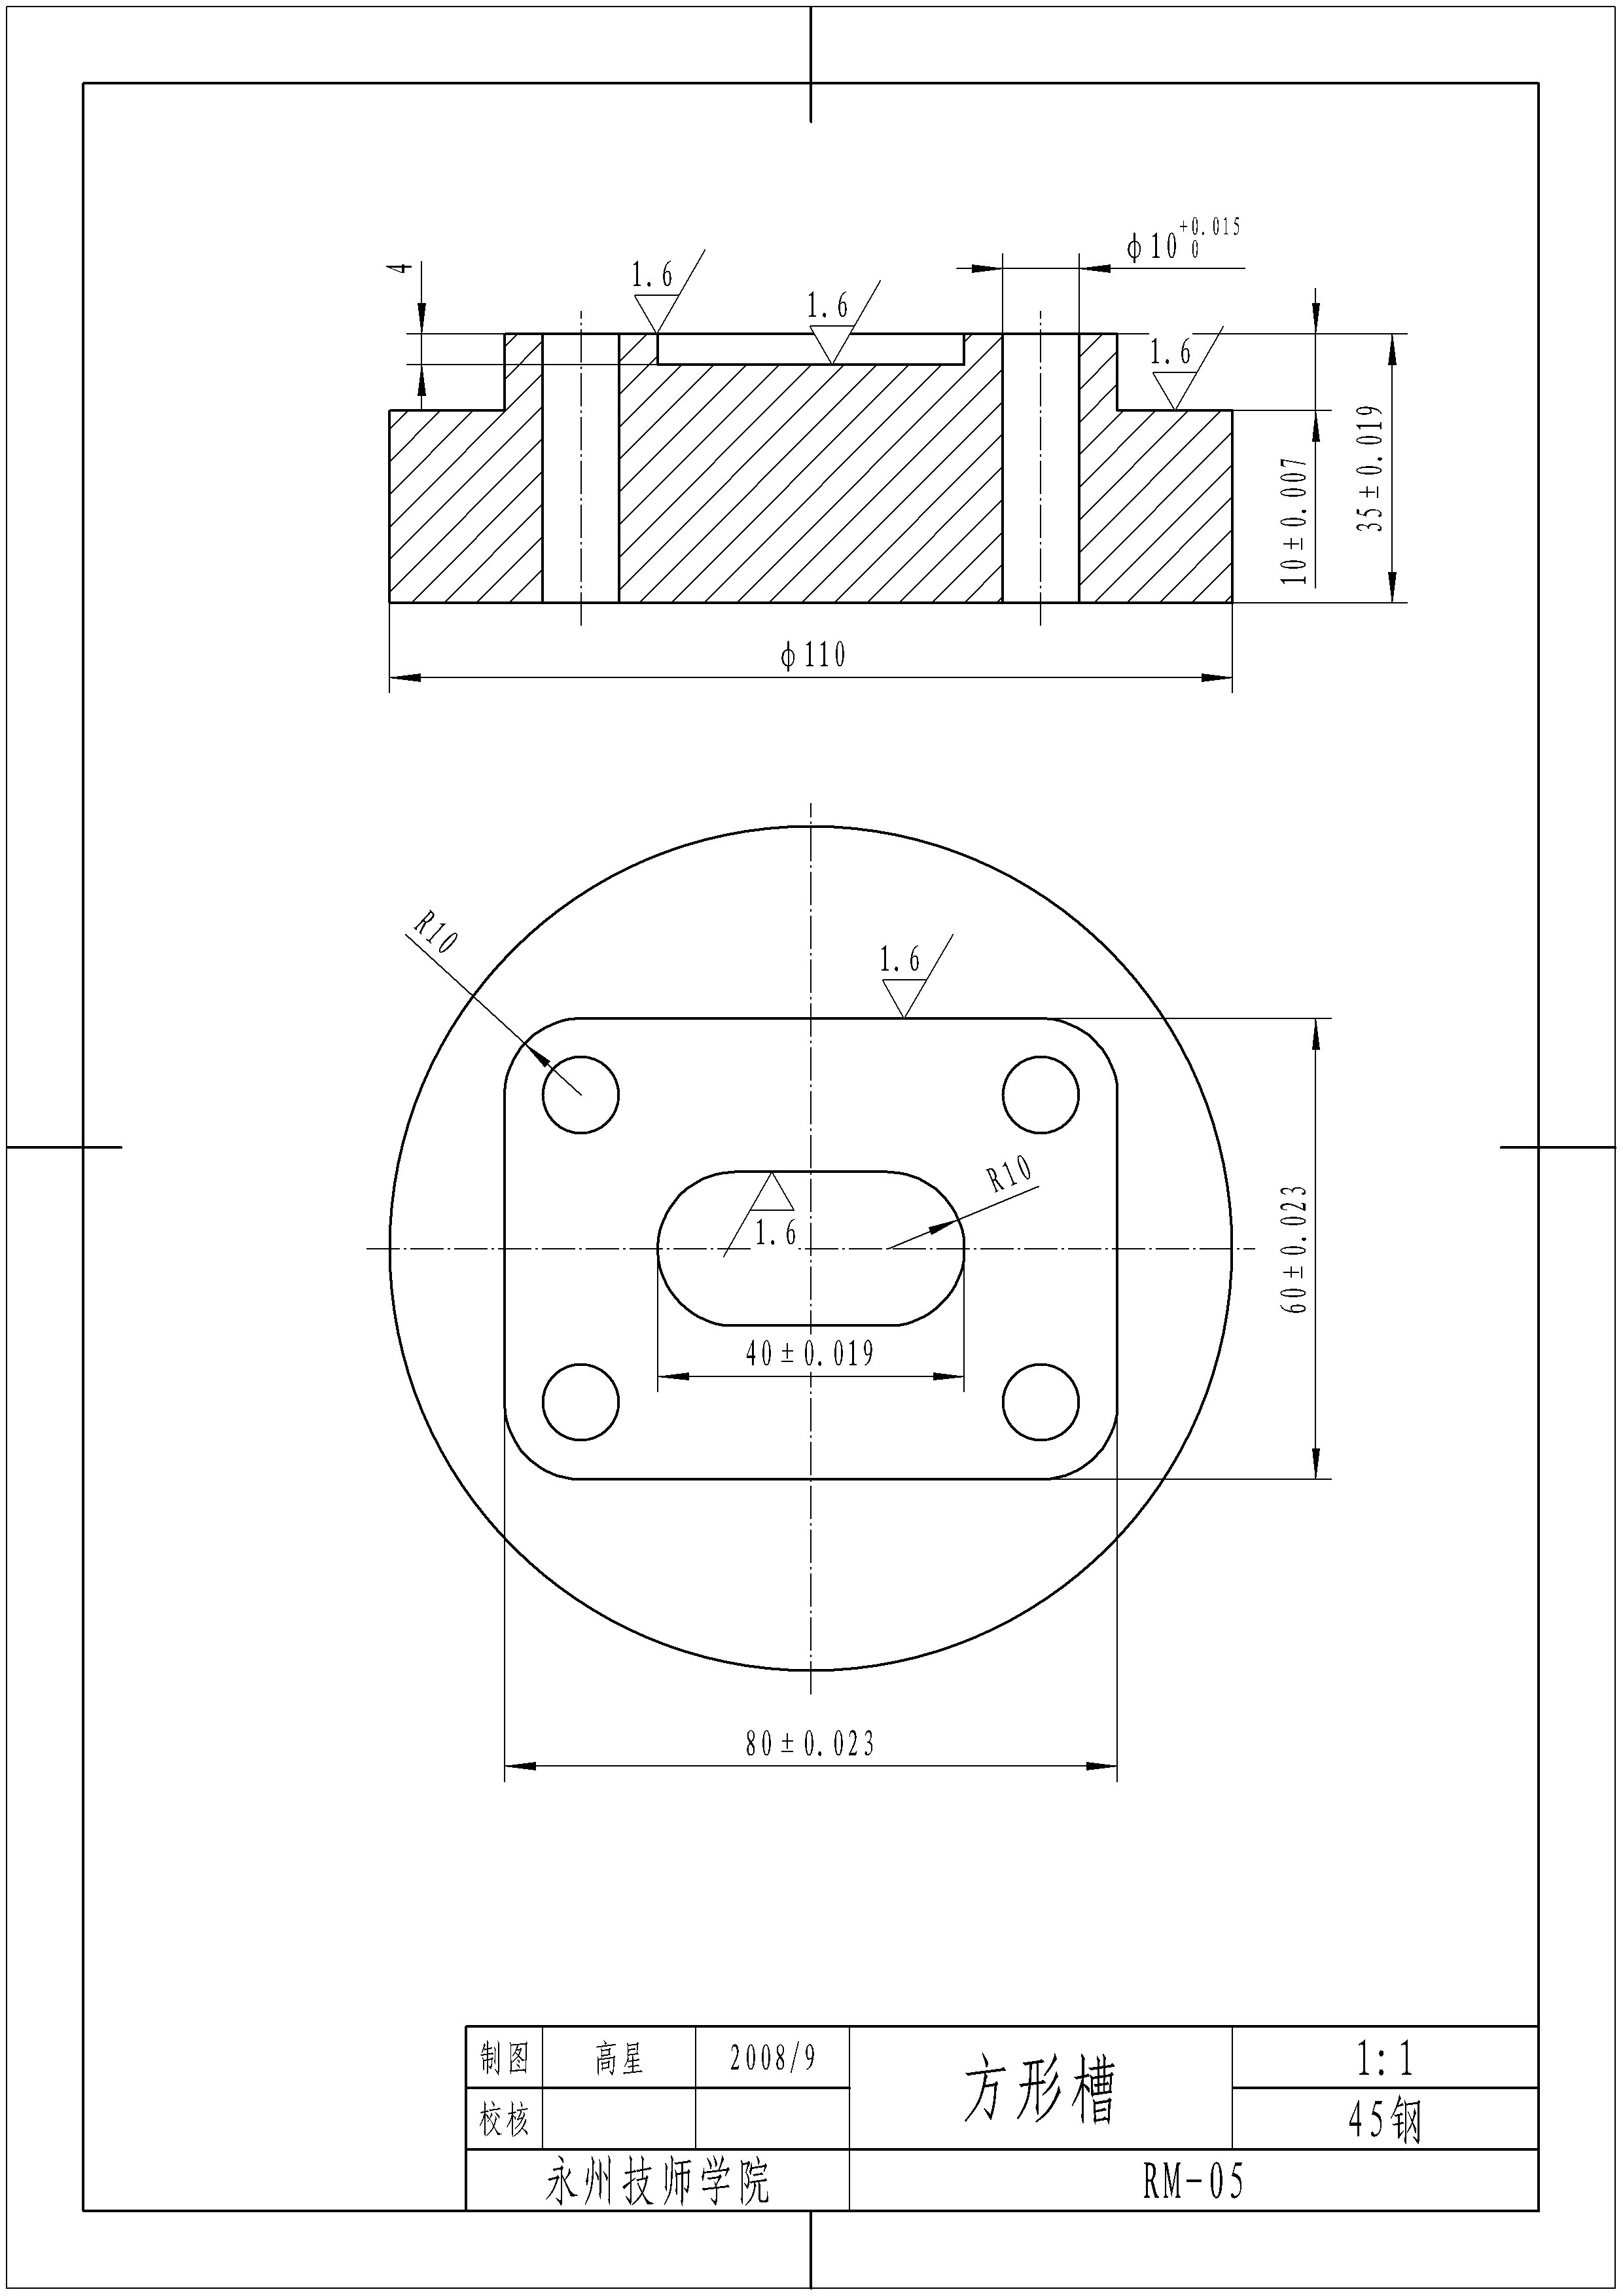
\includegraphics[width=0.7\linewidth]{data/image/26-1}
	\caption{实例}
	\label{fig:26-1}
\end{figure}


1、工件坐标系:工件上表面的中心(面铣后的上表面)

2、装夹:卡盘或平口钳(在两侧加工安装侧面)

3、刀具:

$\varnothing$16三齿立铣刀:面铣、粗加工内外轮廓

$\varnothing$12立铣发:精加工内外轮廓

$\varnothing$5中心钻:钻中心孔

$\varnothing$9.8麻花钻:钻孔

$\varnothing$10机用铰刀:铰孔

4、工序表:

如表\ref{biao:1}

\begin{table}[h]
	\centering
	\caption[表]{工序表}
	\label{biao:1}
\begin{tabular}{|c|c|c|c|c|c|c|}
	\hline 
	1&铣上表面&φ16立铣刀&T1D1&400&200&无\\ 
	\hline 
	2&粗铣外轮廓&φ16立铣刀&T1D1&400&200&\\ 
	\hline
	3&粗铣槽&φ16立铣刀&T1D1&400&200&\\ 
	\hline
	4&钻中心孔&φ5中心钻&T3D1&1200&80&无\\ 
	\hline
	5&钻孔&φ9.8头&T4D1&500&60&无\\ 
	\hline
	6&铰孔&φ10铰刀&T5D1&200&30&无\\ 
	\hline
	7&精铣外轮廓&φ12立铣刀&T2D1&800&120&\\ 
	\hline 
\end{tabular} 
\end{table}

5、走刀路径及相关点坐标

A、面铣: 

B、加工外外轮廓: 

C、内轮廓加工:Z字形下刀。

D:孔加工:

6、参考程序:

\begin{lstlisting}
GX_01(主程序)
G54G17G40G90
T1D1(换16立铣刀)
L11
T3D1(换5中心钻)
L33
T4D1(换9.8钻头)
L41
T5D1(换10铰刀)
L51
T2D1(换12立铣)
L21
M5
\end{lstlisting}


\subsection{课堂小结}
\begin{enumerate}[1、]
\item Siemens 上的换刀;
\item Simens上的长度补偿;
\item 编程实例。
\end{enumerate}

\vfill
\subsection{布置作业}
\begin{enumerate}[1、]
\item 综合习题一。
\end{enumerate}
\vfill
\jxhj{%教学后记
	}
\skrq{%授课日期
	2017年12月14日 4-5节}
\ktmq{%课题名称
	 加工中心编程}
\jxmb{%教学目标,每行前面要加 \item
	\item 掌握加工中心的区别;
	\item 掌握Fanuc加工中心换刀;
	\item 掌握加工中心编程区别;
	\item 会进行加工中心的编程。}
\jxzd{%教学重点,每行前面要加 \item
	\item Fanuc上孔加工指令的使用;
	\item 进行孔加工程序的编写。 }
\jxnd{%教学难点,每行前面要加 \item
	\item 进行孔加工程序的编写。 }
\jjff{%教学方法
	通过讲述、举例、演示法来说明;}

\makeshouye %制作教案首页

%%%%教学内容
\subsection{组织教学}
\begin{enumerate}[\hspace{2em}1、]
	\item 集中学生注意力;
	\item 清查学生人数;
	\item 维持课堂纪律;
\end{enumerate}

\subsection{复习导入及主要内容}
\begin{enumerate}[1、]
\item Siemens 上的换刀;
\item Simens上的长度补偿;
\item 编程实例。
\end{enumerate}

\subsection{教学内容及过程}
\subsubsection{加工中心}

加工中心是指刀库及换刀装置的数控机床
有的基床有可回转的工作台,一边用于加工,一边用于装夹。

刀库的类型:

1、盘式刀库

2、链式刀库

3、盒子刀库

换刀装置:

1、无机械手

2、机械手

\subsubsection{换刀子程序}

例如:T\_\_M98P9000;

换刀子程序如下:
\begin{lstlisting}
O9000
G91
G30Z0     主轴移动至换刀点平面
M06              主轴准停
M28              刀盘进刀
M11              松刀
G28Z0            回原点
M32              寻找所需刀具
G30Z0            
M10              抓紧刀具
M31              刀盘回退
G90              
M99
\end{lstlisting}

\subsubsection{加工实例}

在Siemens的加工中心上加工如图所示的零件。完成工艺分及加工程序的编写:


\begin{figure}[h]
	\centering
	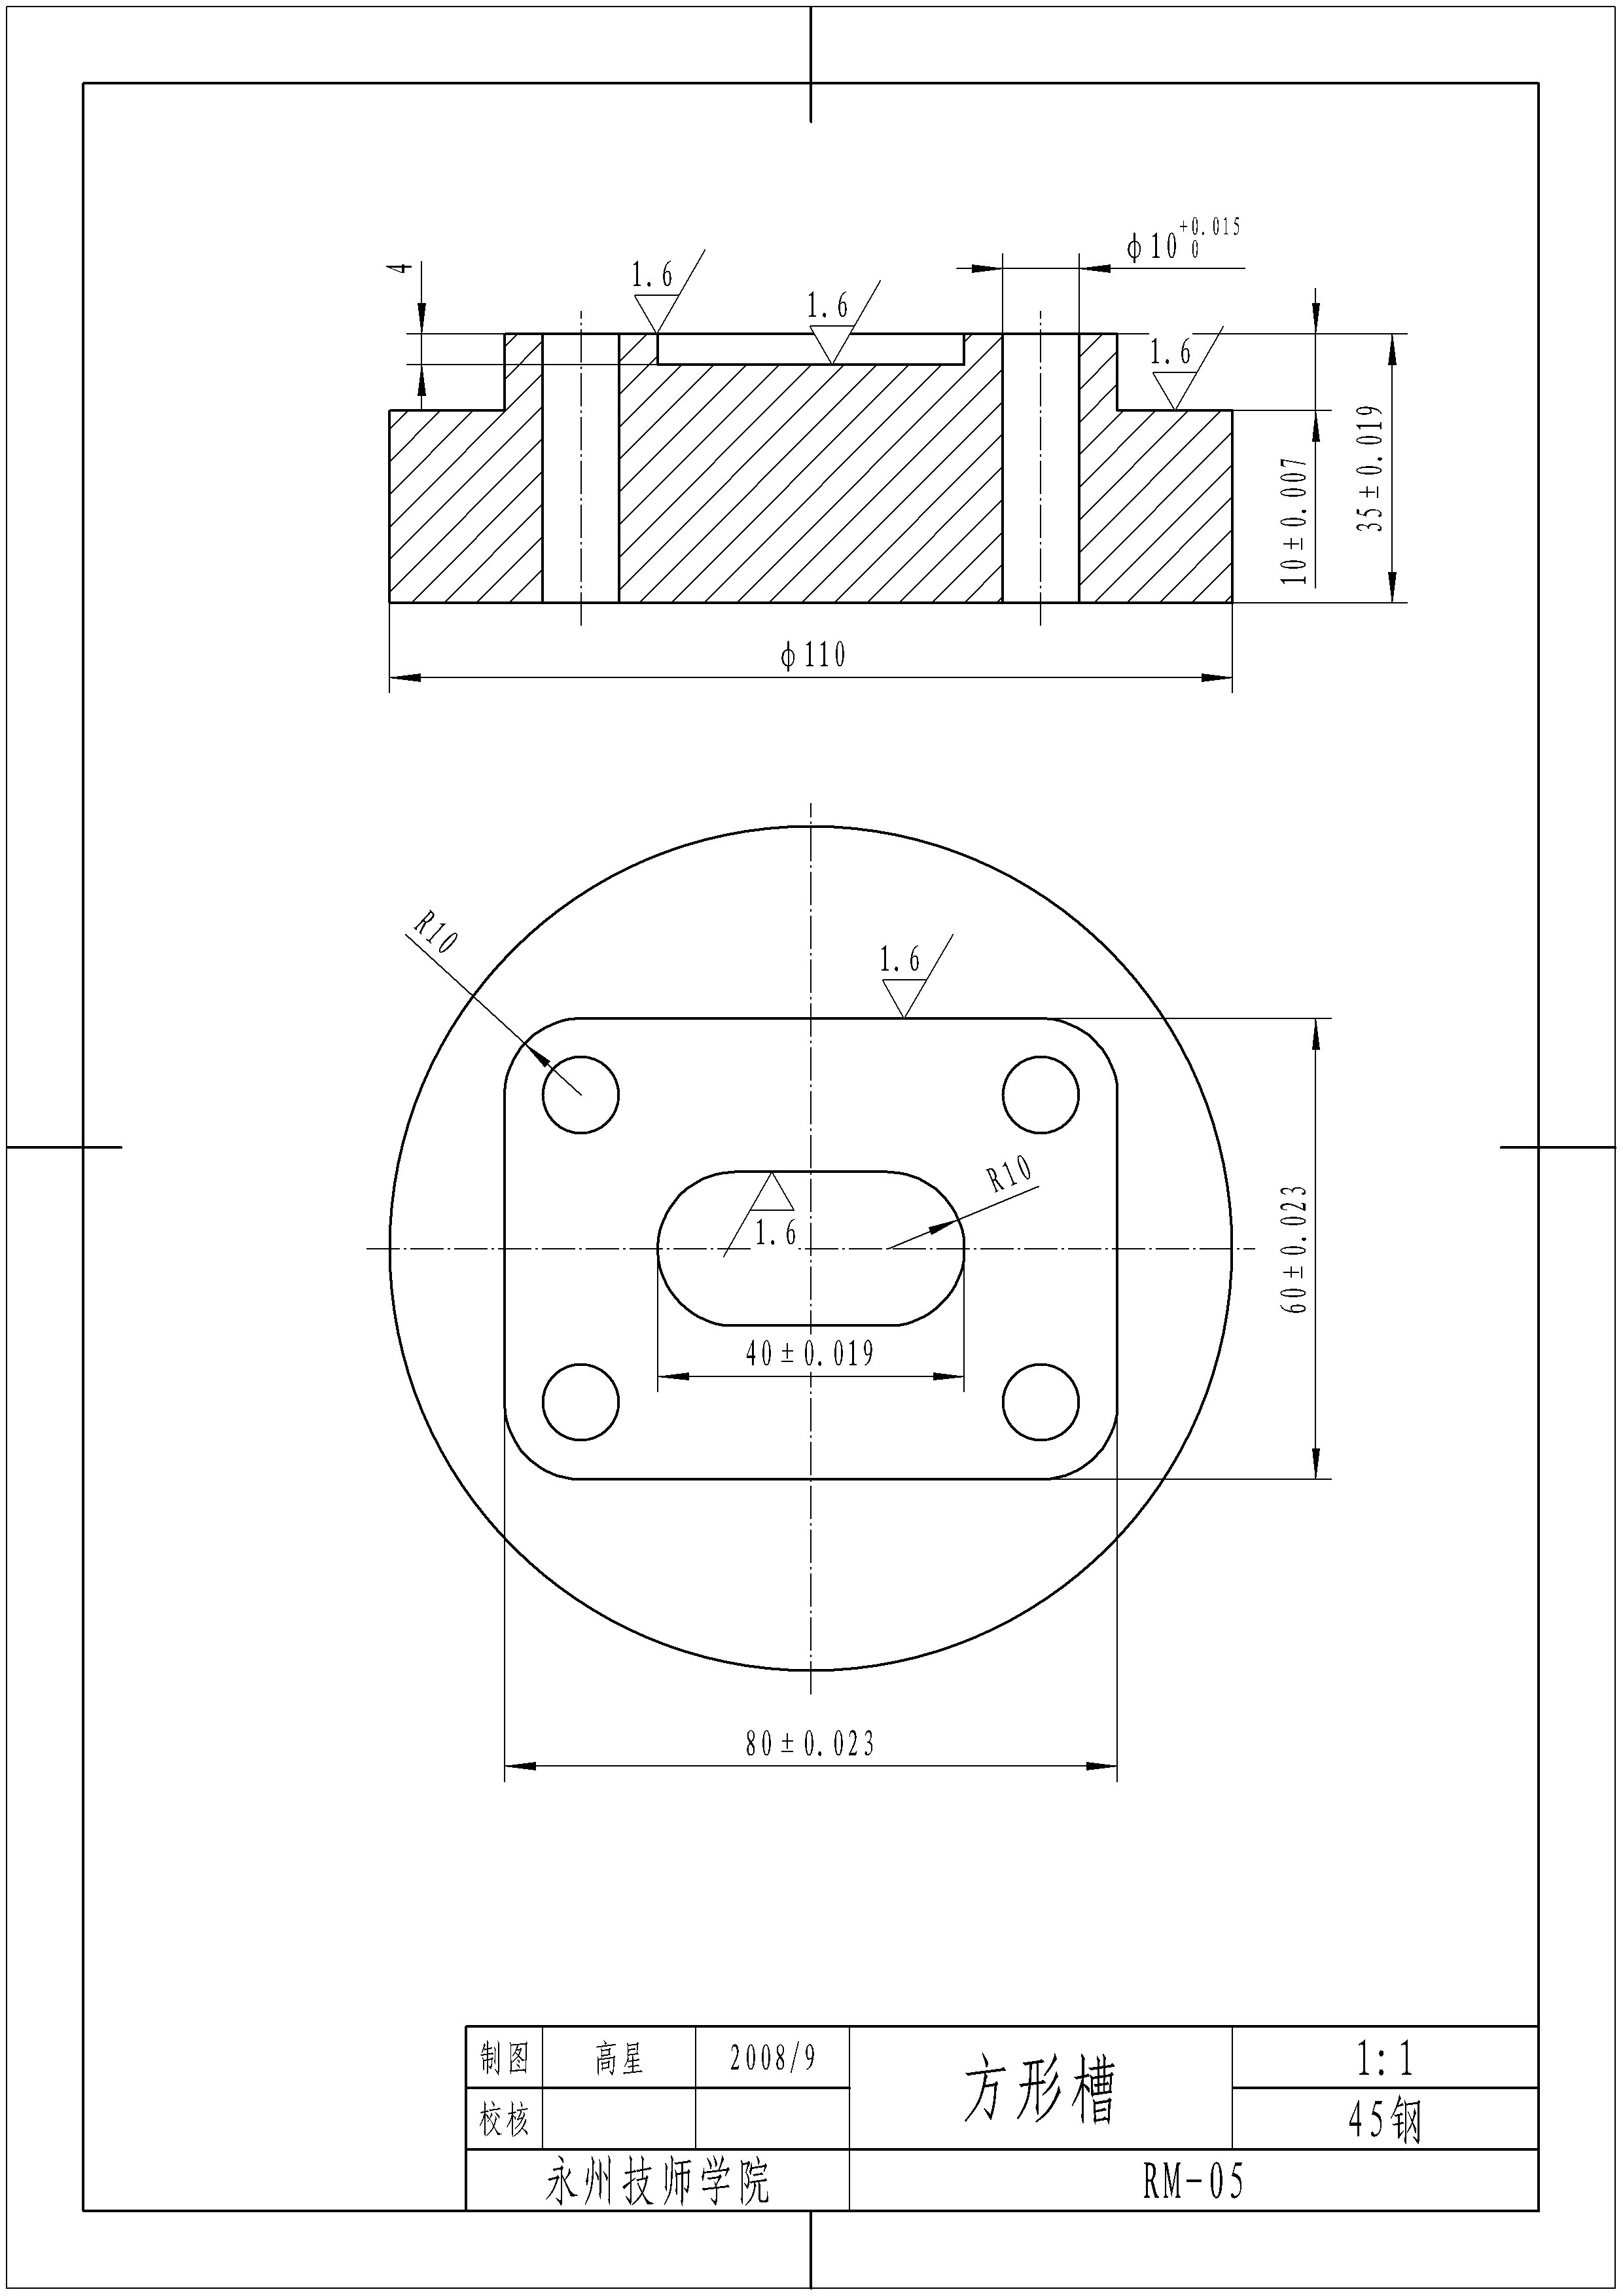
\includegraphics[width=0.7\linewidth]{data/image/26-1}
	\caption{实例}
	\label{fig:26-1}
\end{figure}


1、工件坐标系:工件上表面的中心(面铣后的上表面)

2、装夹:卡盘或平口钳(在两侧加工安装侧面)

3、刀具:

$\varnothing$16三齿立铣刀:面铣、粗加工内外轮廓

$\varnothing$12立铣发:精加工内外轮廓

$\varnothing$5中心钻:钻中心孔

$\varnothing$9.8麻花钻:钻孔

$\varnothing$10机用铰刀:铰孔

4、工序表:

如表\ref{biao:1}

\begin{table}[h]
	\centering
	\caption[表]{工序表}
	\label{biao:1}
	\begin{tabular}{|c|c|c|c|c|c|c|}
		\hline 
		1&铣上表面&φ16立铣刀&T1D1&400&200&无\\ 
		\hline 
		2&粗铣外轮廓&φ16立铣刀&T1D1&400&200&\\ 
		\hline
		3&粗铣槽&φ16立铣刀&T1D1&400&200&\\ 
		\hline
		4&钻中心孔&φ5中心钻&T3D1&1200&80&无\\ 
		\hline
		5&钻孔&φ9.8头&T4D1&500&60&无\\ 
		\hline
		6&铰孔&φ10铰刀&T5D1&200&30&无\\ 
		\hline
		7&精铣外轮廓&φ12立铣刀&T2D1&800&120&\\ 
		\hline 
	\end{tabular} 
\end{table}

5、走刀路径及相关点坐标

A、面铣: 

B、加工外外轮廓: 

C、内轮廓加工:Z字形下刀。

D:孔加工:

6、参考程序:

\begin{lstlisting}
GX_01(主程序)
G54G17G40G90
T1D1(换16立铣刀)
L11
T3D1(换5中心钻)
L33
T4D1(换9.8钻头)
L41
T5D1(换10铰刀)
L51
T2D1(换12立铣)
L21
M5
\end{lstlisting}



\subsection{课堂小结}
\begin{enumerate}[1、]
\item 加工中心概述;
\item Fanuc加工中心换刀;
\item Fanuc数铣换刀;
\item 编程实例。
\end{enumerate}

\vfill
\subsection{布置作业}
\begin{enumerate}[1、]
	\item 综合习题一。
\end{enumerate}
\vfill
\jxhj{%教学后记
	}
\skrq{%授课日期
	2017年12月19日 4-5节}
\ktmq{%课题名称
	 倒角与倒圆角}
\jxmb{%教学目标,每行前面要加 \item
	\item 掌握FANUC上的倒角与拐圆角指令;
	\item 掌握Siemens上的倒角与拐圆角;
	\item 掌握倒角与拐圆角编程。
}
\jxzd{%教学重点,每行前面要加 \item
	\item 掌握FANUC上的倒角与拐圆角指令;
	\item 掌握Siemens上的倒角与拐圆角。 }
\jxnd{%教学难点,每行前面要加 \item
	\item 掌握倒角与拐圆角编程。 }
\jjff{%教学方法
	通过讲述、举例、演示法来说明;}

\makeshouye %制作教案首页

%%%%教学内容
\subsection{组织教学}
\begin{enumerate}[\hspace{2em}1、]
	\item 集中学生注意力;
	\item 清查学生人数;
	\item 维持课堂纪律;
\end{enumerate}

\subsection{复习导入及主要内容}
\begin{enumerate}[1、]
\item 加工中心概述;
\item Fanuc加工中心换刀;
\item Fanuc数铣换刀;
\item 编程实例。
\end{enumerate}

\subsection{教学内容及过程}

倒角及倒圆角是数控铣削、加工中心中常见的结构,利用数控系统中的倒圆角,倒角指令可以使程序的编制简化。
\begin{figure}[h]
	\centering
	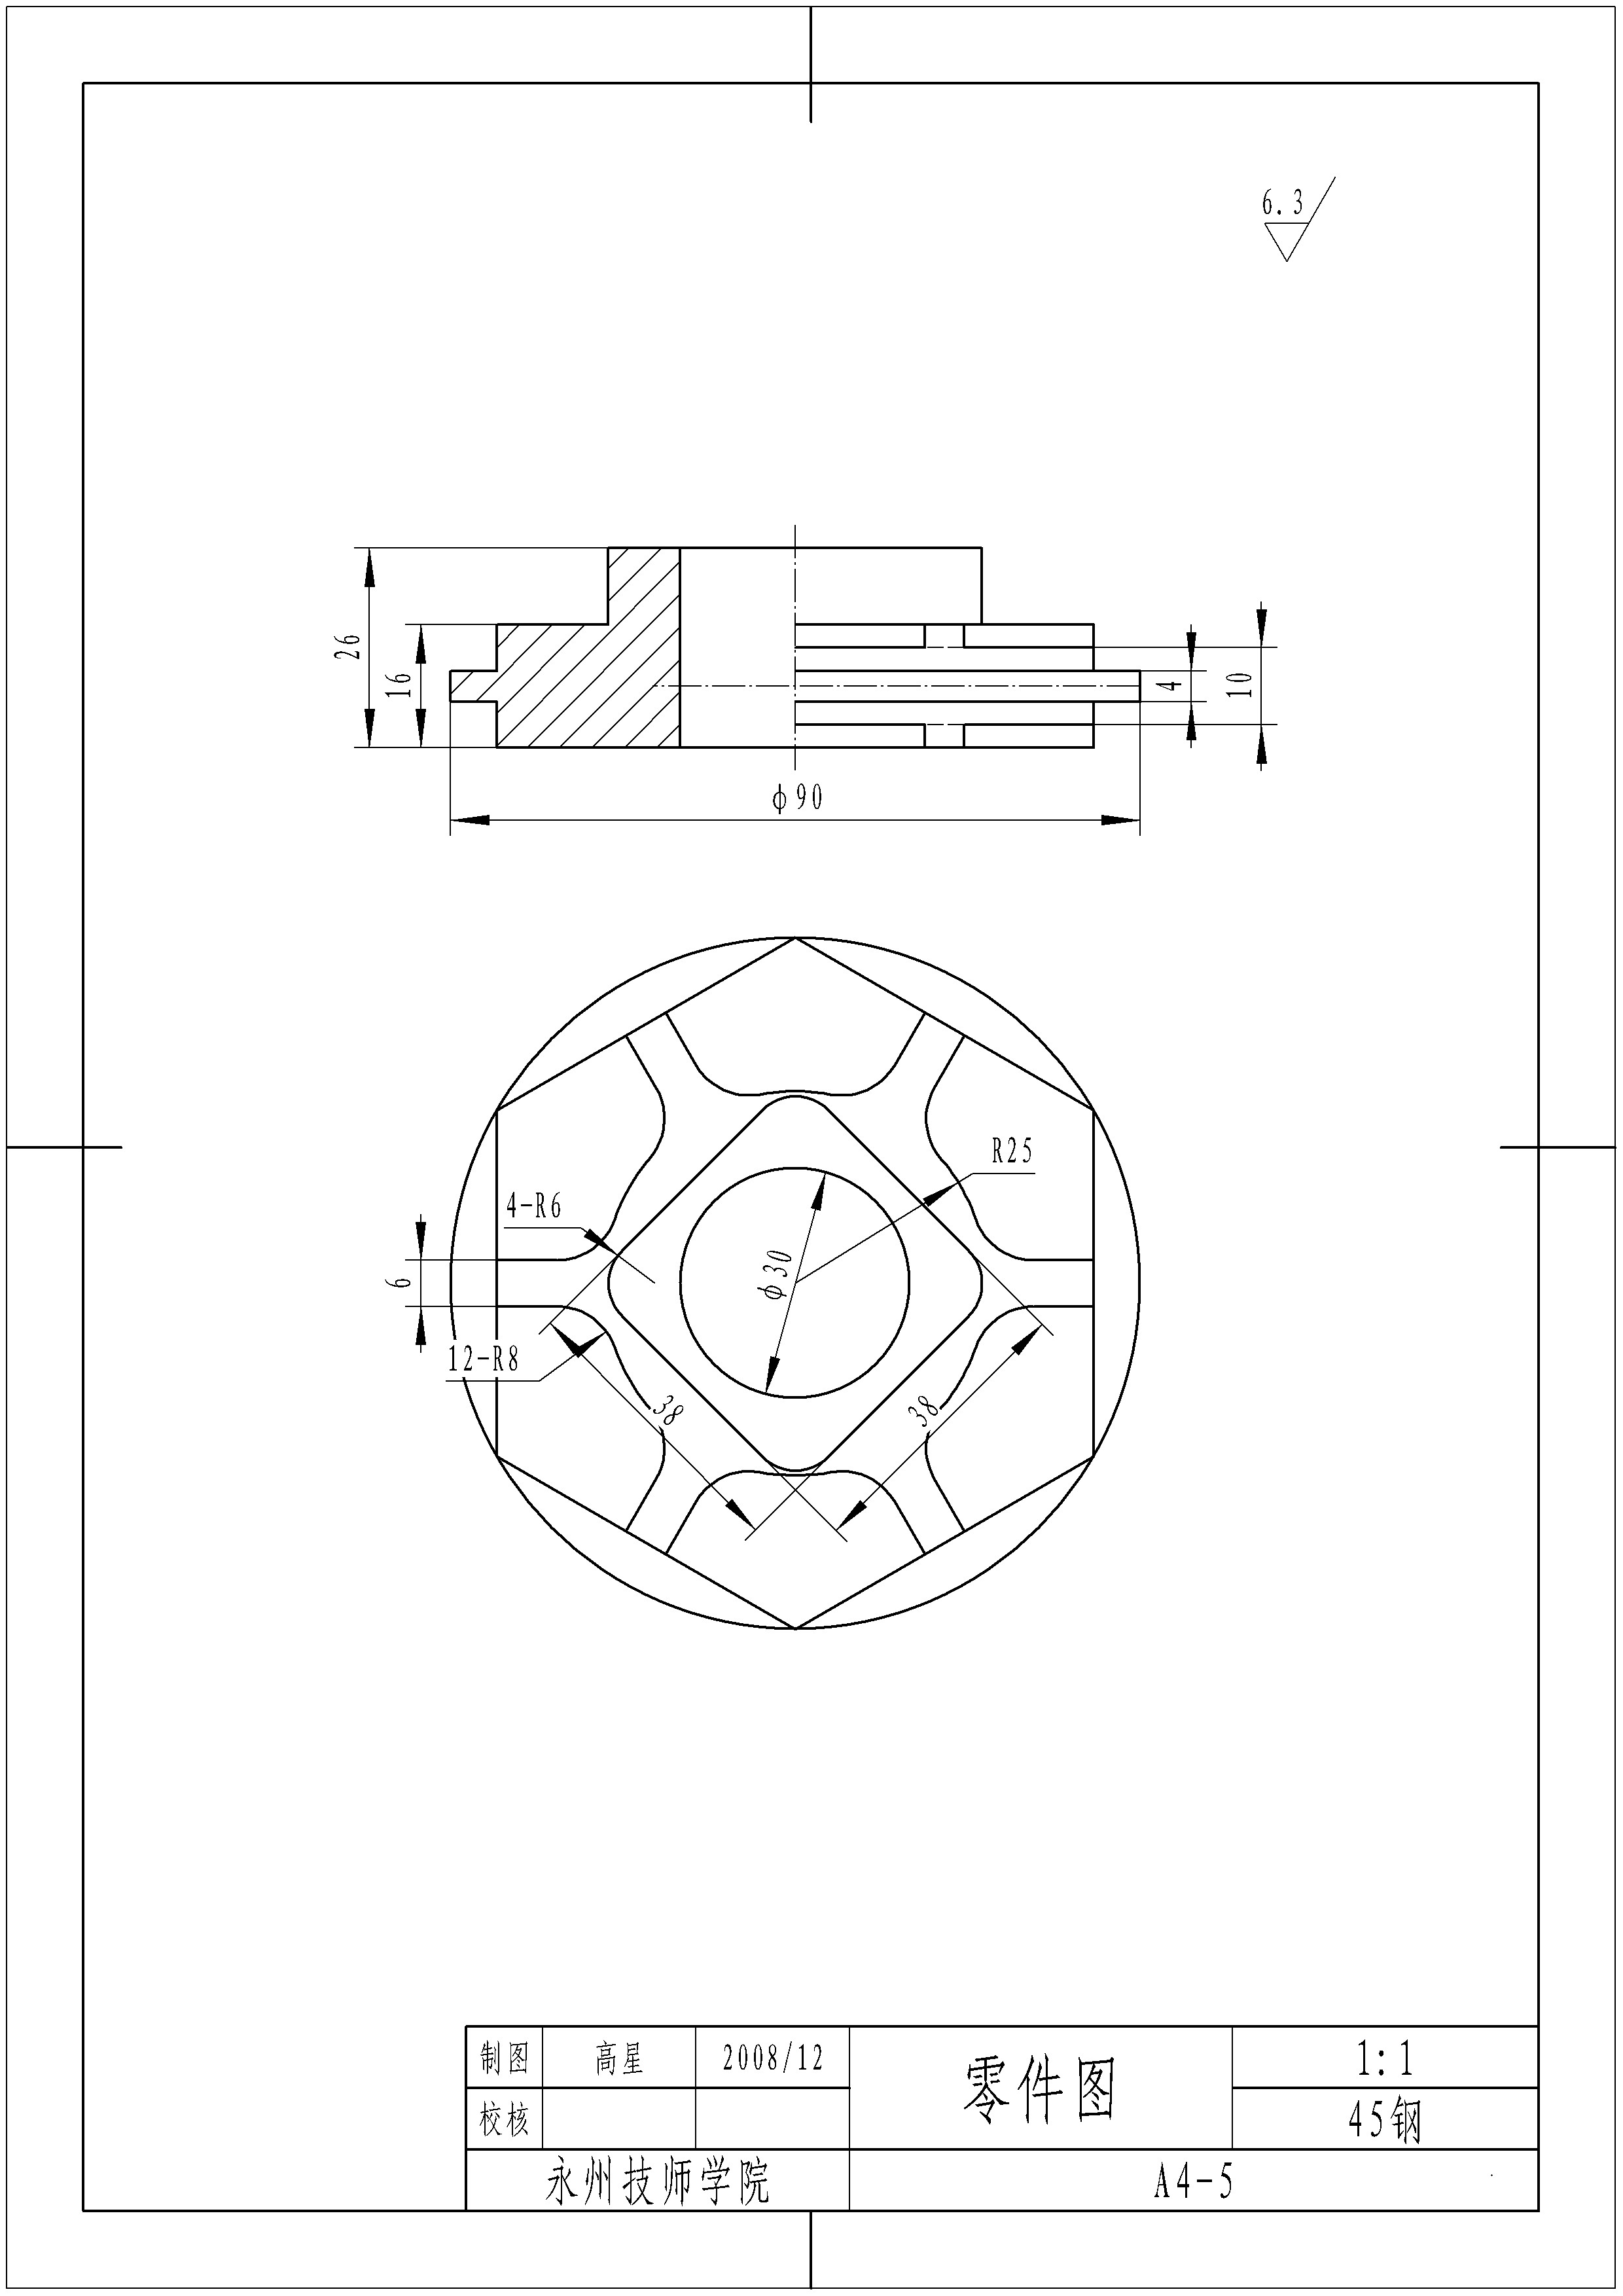
\includegraphics[width=0.8\linewidth,trim=100 200 100  200,clip]{data/image/28-1}
	\caption{示例}
	\label{fig:28-1}
\end{figure}

\begin{figure}[h]
	\centering
	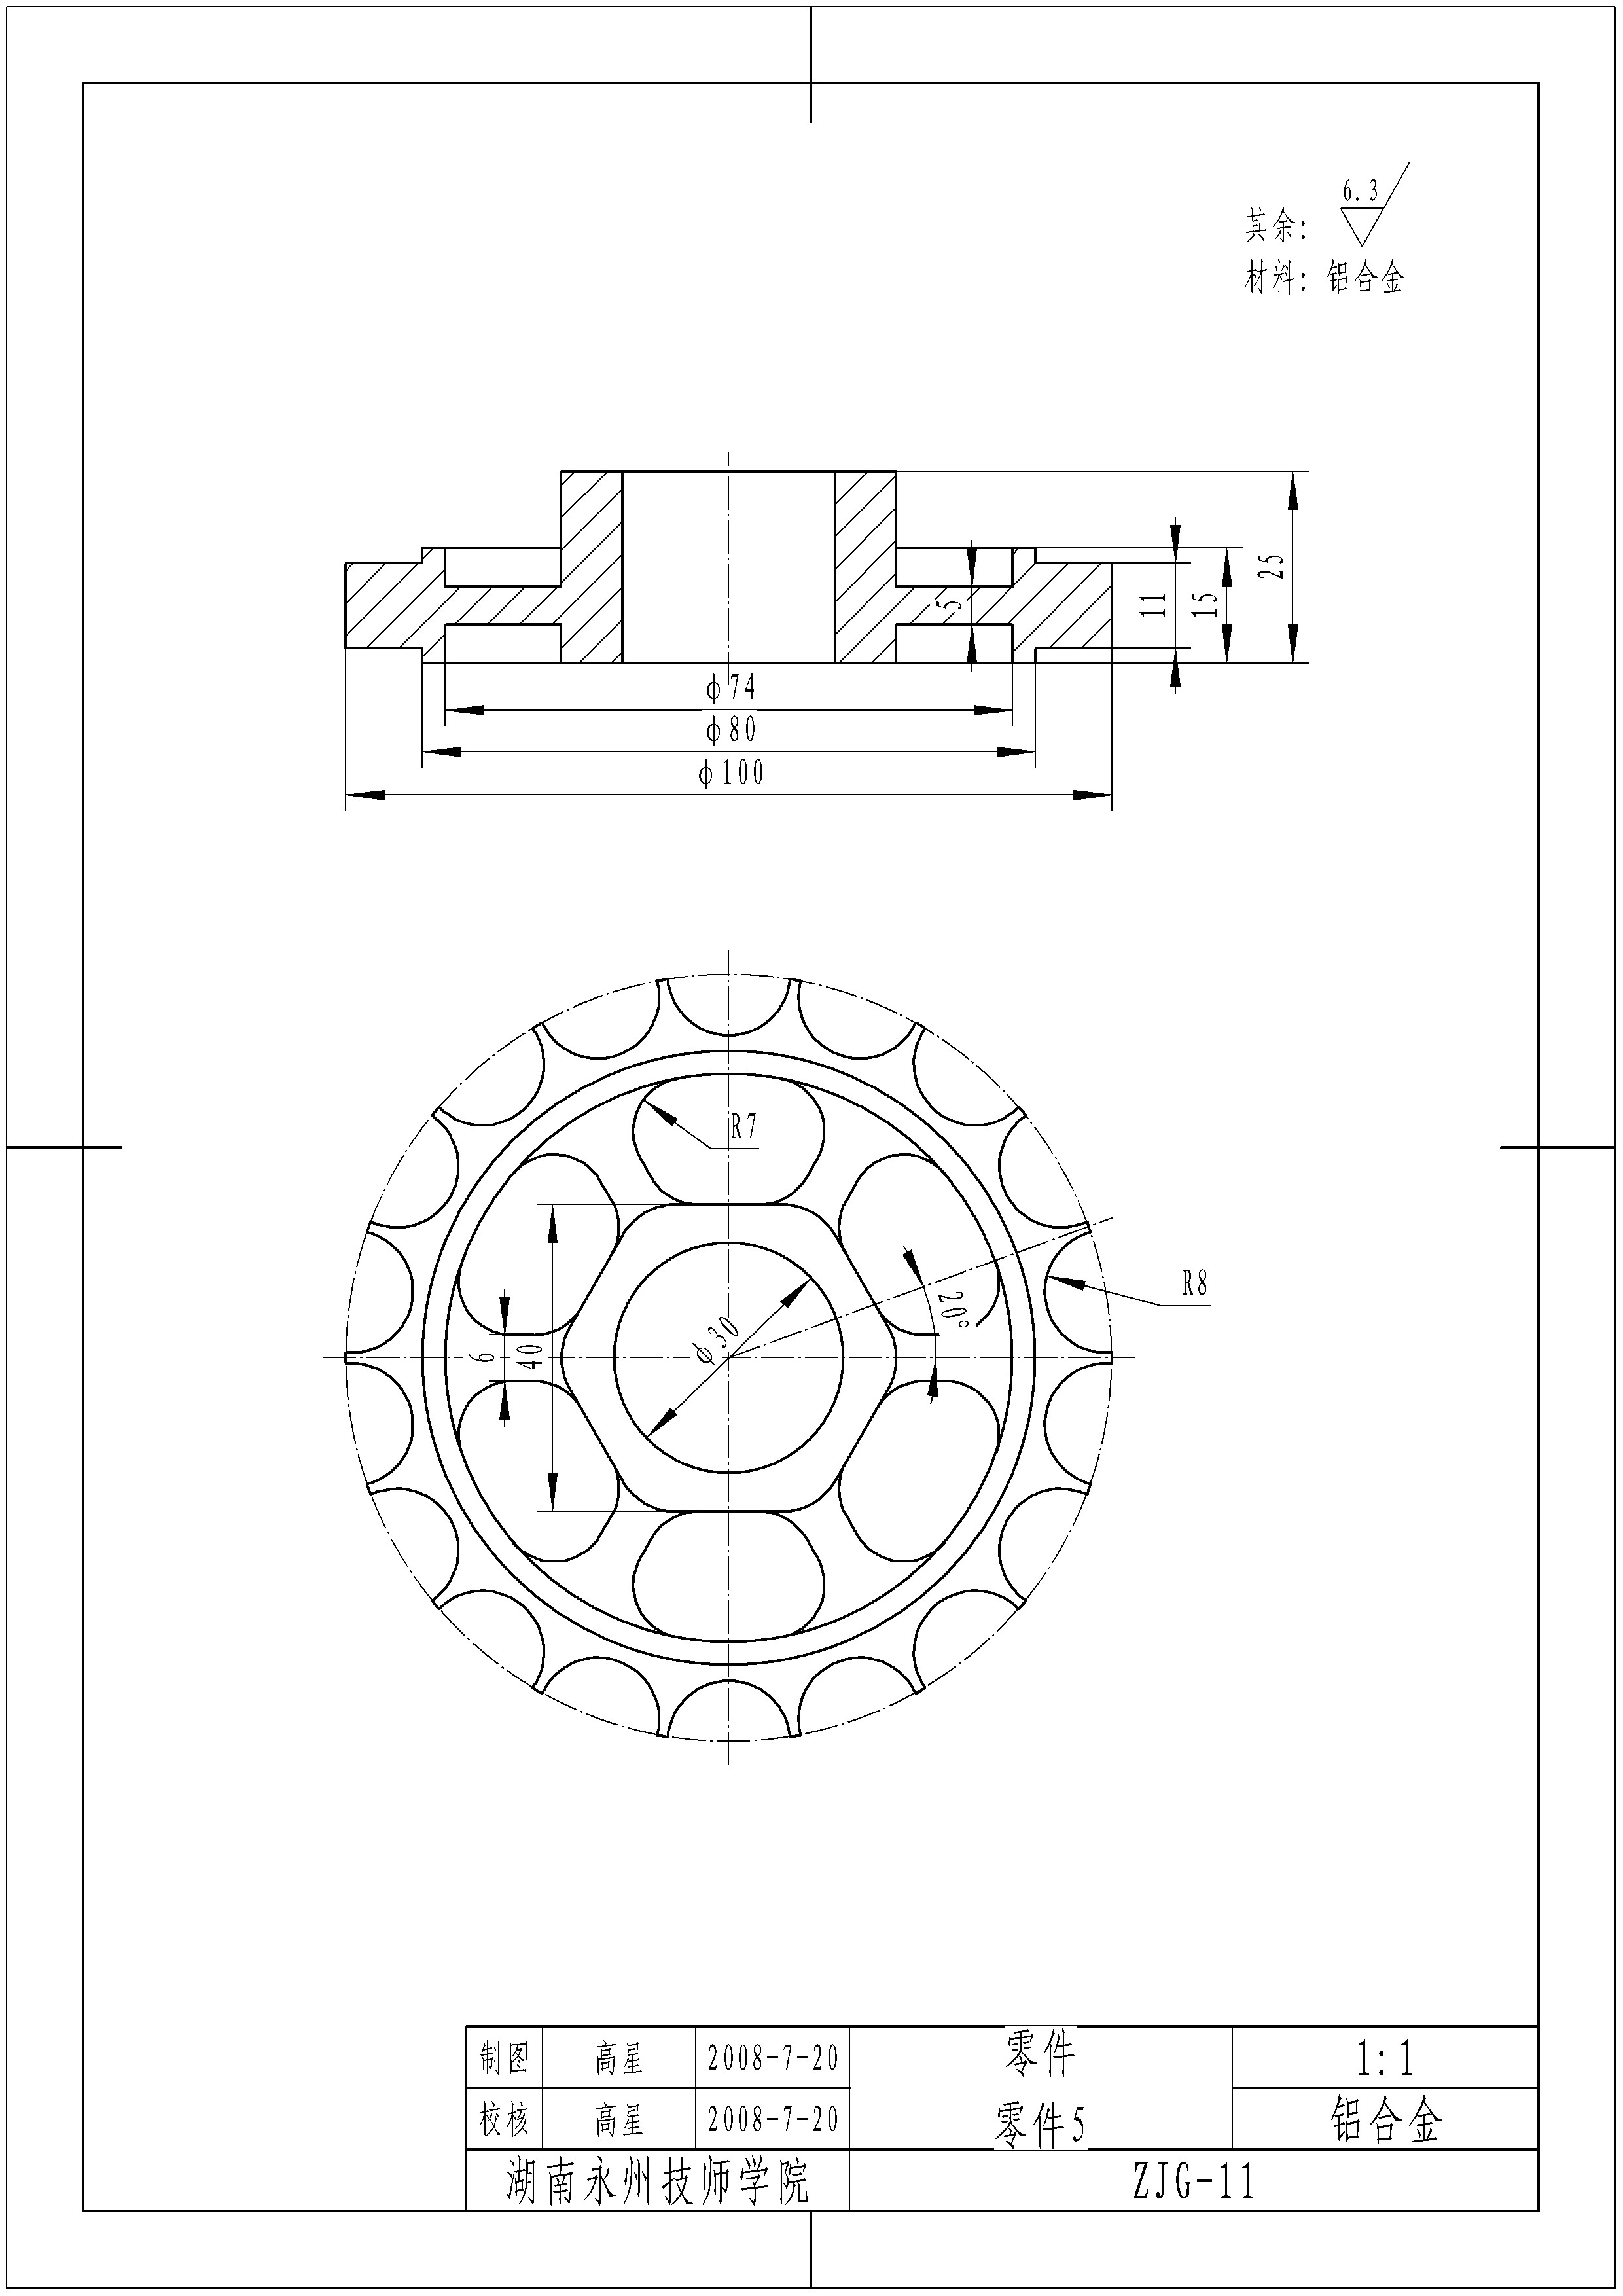
\includegraphics[width=0.8\linewidth,trim=100 200 100  150,clip]{data/image/28-2}
	\caption{示例}
	\label{fig:28-2}
\end{figure}

\subsubsection{Fanuc上的倒角、倒圆角的指令格式}
	
1、在直线插补G1或圆弧插补G2、G3程序段的末尾,加上倒角或倒圆角的指令:

……,C\_\_\_\_;(倒角)

……,R\_\_\_\_;(倒圆角)

2、可以用在以下的程序段之间:

在直线插补和直线插补程序段之间

在直线插补和圆弧插补程序段之间

在圆弧插补和直线插补程序段之间

在圆弧插补和圆弧插补程序段之间

3、应用条件:

直线与直线、直线与圆弧、圆弧与圆弧要有虚拟交点

虚拟交点坐标已知或方便求出

因为编程时,直线插补、圆弧插补的目标点必须是它们的虚拟交点。

4、说明:

A、倒角和拐角圆弧过渡只能在G17、G18、G19指定的平面内执行。

B、指定倒角或拐圆角过渡的程序段的下一个程序段必须跟随一个用直线插补G1或圆弧插补G2、G3指令的程序段,如果下一个程序段不包含这些指令,系统会出现报警。

C、在平面切换之后,被指定的程序段中不能指定倒角或倒圆角。

D、如果插入的倒角或圆弧过渡的程序段引起刀具超过原插补移动的范围,系统会发出报警。

E、在坐标系变动G92或G52到G59或执行返回参考点G28到G30之后的程序段中不能指定倒角或圆角过渡。

F、圆角过度不能在螺纹加工程序段中指定

G、DNC操作不能使用任意角度倒角和拐角圆弧过渡。
倒角及倒圆角是数控铣削、加工中心中常见的结构,利用数控系统中的倒圆角,倒角指令可以使程序的编制简化。
	
	
	
	
	
	


\subsubsection{Siemens上的倒角、倒圆角的指令格式}
	1、在直线插补G1或圆弧插补G2、G3程序段的末尾,加上倒角或倒圆角的指令:
	
	……CHR=\_\_\_\_(倒角,与Fanuc中的C一样)
	
	……CHF=\_\_\_\_(倒角,数值为倒角边的长度)
	
	……RND=\_\_\_\_(倒圆角)
	
	2、可以用在以下的程序段之间:
	
	在直线插补和直线插补程序段之间
	
	在直线插补和圆弧插补程序段之间
	
	在圆弧插补和直线插补程序段之间
	
	在圆弧插补和圆弧插补程序段之间
	
	3、应用条件:
	
	直线与直线、直线与圆弧、圆弧与圆弧要有虚拟交点
	
	虚拟交点坐标已知或方便求出
	
	因为编程时,直线插补、圆弧插补的目标点必须是它们的虚拟交点。
	
	4、说明:
	
	A、在程序段中若轮廓长度不够,则会自动地削减倒角和倒圆的的编程值。

	B、如果连续编程的程序段超过3段没有运行指令,不插入倒角、倒圆。

	C、如果更换平面不插入倒角、倒圆。
	

\subsubsection{编程实例}
\begin{lstlisting}
O1 FANUC
G54G17G40G49G90
M3S500
G43G1Z100.H1F2000
X-100.Y0
Z5.0
Z-5.0F200
G1G41X-50.Y-10.D1
G3X-40.Y0R10.
G1Y30.;R8.0
X40.;R8.0
Y-30.;R8.0
X-40.;R8.0
Y0
G3X-50.Y0R10
G40G1X-100.Y0
G1Z100.F2000
G49G1Z150.
M5
M30
GX01   SIEMENS 
G54G17G40GG90
T1D1
M3S500
G1Z100.F2000
X-100.Y0
Z5.0
Z-5.0F200
G1G41X-50.Y-10.D1
G3X-40.Y0CR=10.
G1Y30.RAN=8.0
X40.RAN=R8.0
Y-30.RAN=R8.0
X-40.RAN=R8.0
Y0
G3X-50.Y0R10
G40G1X-100.Y0
G1Z100.F2000
G49G1Z150.
M5
M30
\end{lstlisting}


\subsection{课堂小结}
\begin{enumerate}[1、]
\item Fanuc上的倒角、倒圆角的指令格式;
\item Siemens上的倒角、倒圆角的指令格式;
\item 编程实例。
\end{enumerate}

\vfill
\subsection{布置作业}
\begin{enumerate}[1、]
	\item 综合习题一。
\end{enumerate}
\vfill
\jxhj{%教学后记
	}
\skrq{%授课日期
	2017年12月21日 4-5节}
\ktmq{%课题名称
	 局部坐标系}
\jxmb{%教学目标,每行前面要加 \item
	\item 掌握Fanuc上G52指令的格式;
	\item 掌握Siemens上Trans指令的格式;
	\item 掌握用局部坐标系指令编程。
}
\jxzd{%教学重点,每行前面要加 \item
	\item 掌握Fanuc上G52指令的格式;
	\item 掌握用局部坐标系指令编程。 }
\jxnd{%教学难点,每行前面要加 \item
	\item 掌握用局部坐标系指令编程。 }
\jjff{%教学方法
	通过讲述、举例、演示法来说明;}

\makeshouye %制作教案首页

%%%%教学内容
\subsection{组织教学}
\begin{enumerate}[\hspace{2em}1、]
	\item 集中学生注意力;
	\item 清查学生人数;
	\item 维持课堂纪律;
\end{enumerate}

\subsection{复习导入及主要内容}
\begin{enumerate}[1、]
\item Fanuc上的倒角、倒圆角的指令格式;
\item Siemens上的倒角、倒圆角的指令格式;
\item 编程实例。
\end{enumerate}

\subsection{教学内容及过程}
\subsubsection{几种坐标系}
	1、工件坐标系:G54-G59、G92
	
	G54-G59是在机床参数中以机床坐标为基准设定工件坐标系

	G92是在程序中以刀具当前位置为基准设定工件坐标系

	一般使用G54~G59指令后,就不再使用G92指令。

	2、机床坐标系:G53

	当需要用机床坐标系编程时,用G53指令。

	机床坐标系通过回零(回参考点)建立。

	如坐标系不对,可通过回零重新建立机床坐标系,机床坐标系原点在机床上是固定的一个点,这个点不会变的。

	3、局部坐标系:G52、Trans

	在工件坐标上建立一个子工件坐标系。即局部坐标系。


\subsubsection{Fanuc上局部坐标系}
	指令格式:  G52 X\_ Y\_ Z\_;建立局部坐标系

	G52 X0 Y0 Z0 ;取消局部坐标系。

	说明:其X、Y的定义是原坐标系的程序原点到子坐标系的程序原点之向量值。

	G52 X0 Y0;=>表示回复到原坐标系。

	注意:

	1、局部坐标系设定不改变工件和机床坐标系。 

	2、当用G50定义工件坐标系时,如果没有对局部坐标系中的所有轴指定坐标值,局部坐标系保持不变。如果没有为局部坐标系中的任何轴指定坐标值,局部坐标系被取消。 

	3、G52暂时取消刀尖半径补偿中的偏移。 

	4、在绝对方式紧跟G52之后指令一个运动指令。 

	5、复位时是否取消局部坐标系取决于参数的设定。当3402号参数的第6位(CLR)或者1202号参数3位(RLC)设为1时,局部坐标系在复位状态被取消。 

	6、手动返回参考点是否取消局部坐标系取决于ZCL的设定(参数1201的第2位)。

\subsubsection{Siemens上的局部坐标系}

	指令格式:

	TRANS X\_ Y\_ Z\_ ;可编程的偏移,清除所有有关偏移、旋转、比例系数、镜像的指令 

	ATRANS X\_ Y\_ Z\_ ;可编程的偏移,附加于当前的指令 

	TRANS;不带数值清除所有有关偏移、旋转、比例系数、镜像的指令 

	TRANS/ATRANS 指令要求一个独立的程序段。

	四、编程实例:

	在数控机床上加工如图所示的零件,完成工艺分析及加工程序的编写。
	
	\begin{figure}
		\centering
		\includegraphics[width=0.9\linewidth,trim=50 285 50  250,clip]{data/image/29-1}
		\caption{加工实例}
		\label{fig:29-1}
	\end{figure}

1、工件坐标系:

2、装夹

3、刀具:

$\varnothing$12立铣刀

$\varnothing$8立铣刀

4、加工顺序

	
\subsubsection{如图\ref{fig:29-2}所示,加工40*40矩形凸台,高3mm,刀具为Ф14的平底刀。}

	\begin{figure}
	\centering
	\includegraphics[width=0.9\linewidth,trim=0 0 0 0,clip]{data/image/29-2}
	\caption{加工实例}
	\label{fig:29-2}
\end{figure}

分析:

(1)凸台为倾斜形式,可以使用旋转指令编程。

(2)凸台四角带圆角,可以使用倒圆角指令编程。

(3)使用局部坐标系,将当前工件坐标系移至凸台的中心处。

加工程序如下:

\begin{lstlisting}
O1(FANUC)
G54G17G90G40
G01Z100F2000
M03S500
G52X100Y80            当前工件坐标系移至凸台的中心处
G68X0Y0R-30           当前工件坐标系顺时针旋转30度
G00X-35Y0
G01Z-3F1000            
G01G41X-30Y-10D01
G03X-20Y0R10
G01Y15,R5              倒圆角R5
X20,R5
Y-15,R5
X-20,R2
Y0
G03X-30Y10R10
G01G40X-35Y0
G01Z100F2000
G69                    取消坐标系旋转
G52X0Y0               取消坐标系平移
M05
M30
\end{lstlisting}


\subsection{课堂小结}
\begin{enumerate}[1、]
\item 几种坐标系;
\item Fanuc 上局部坐标系;
\item Siemens 上局部坐标系;
\item 编程实例。
\end{enumerate}

\vfill
\subsection{布置作业}
\begin{enumerate}[1、]
	\item 综合习题一。
\end{enumerate}
\vfill
\jxhj{%教学后记
	}
\skrq{%授课日期
	2017年12月26日 4-5节}
\ktmq{%课题名称
	 极坐标指令与实例}
\jxmb{%教学目标,每行前面要加 \item
	\item 掌握Fanuc上极坐标指令的使用;
	\item 掌握Siemens上极坐标指令的使用;
	\item 灵活使用极坐标指令进行编程;
	\item 掌握加工工艺的分析。
}
\jxzd{%教学重点,每行前面要加 \item
	\item Fanuc上极坐标指令的使用;
	\item Siemens上极坐标指令的使用。 }
\jxnd{%教学难点,每行前面要加 \item
	\item 使用极坐标指令进行编程。 }
\jjff{%教学方法
	通过讲述、举例、演示法来说明;}

\makeshouye %制作教案首页

%%%%教学内容
\subsection{组织教学}
\begin{enumerate}[\hspace{2em}1、]
	\item 集中学生注意力;
	\item 清查学生人数;
	\item 维持课堂纪律;
\end{enumerate}

\subsection{复习导入及主要内容}
\begin{enumerate}[1、]
\item 几种坐标系;
\item Fanuc 上局部坐标系;
\item Siemens 上局部坐标系;
\item 编程实例。
\end{enumerate}

\subsection{教学内容及过程}
\subsubsection{加工轮廓的处理}

\begin{figure}
	\centering
	\includegraphics[width=0.9\linewidth,trim=50 150 50  50,clip]{data/image/30-1}
	\caption{加工轮廓的处理}
	\label{fig:30-1}
\end{figure}

1、加工轮廓的处理(改路径,延长)

把加工轮廓进行拆分

A、两个直槽:

标点的坐标,直角坐标(开放的)

B、小圆弧槽:

标点的坐标,使用极坐标

C、腰形槽:

标点的坐标,极坐标

D、扇形台阶

标点的坐标,极坐标

起点与终点不重合

编程时的处理

E、带翅膀的圆弧槽。

极坐标 与 直角坐标的互换。

X=P*cosA

Y=P*sinA

P=X2+Y2

A=aictanY/X

\subsubsection{极坐标}

1、Fanuc上的极坐标

指令格式: G\_\_ G~~ G16;启动极坐标指令(极坐标方式)
G~~ IP\_\_; 极坐标指令
:

G15;取消极坐标

说明:G\_\_ 极坐标指令的平面选择(G17、G18、G19)

G~~ G90指定工件坐标系的零点作为极坐标系原点,

G91指定当前位置作为极坐标系的原点。

IP\_\_\_ 指定极坐标系选择平面的轴地址及其值。

第1轴:极坐标半径

第2轴:极坐标角度 

用G90指定半径,极点设在工件坐标系原点。

如再用G90指定角度,角度是与X轴的夹角

如再用G91指定角度,角度是与当前位置的夹角

用G91指定半径,极点设在刀具当前位置。

如再用G90指定角度,角度是与X轴的夹角

如再用G91指定角度,角度是与当前位置的夹角。

限制:A、在极坐标方式中,对圆弧插补或螺旋线插补(G02,G03)用R 指定半径。

B、在极坐标方式中,不能用以下指令:

G4、G10、G52、G92、G53、G68、G51

C、在极坐标方式中不能倒角和倒圆

2、Siemens上的极坐标

1、极坐标,极点定义:G110,G111,G112 

A、在直角坐标系中定义极点:

G110/G111/G112 X\_\_ Y\_\_ Z\_\_ 

B、在极坐标系中定义极点:

G110/G111/G112 AP=\_\_\_ RP=\_\_\_

说明: 

G110:相对于刀具最近到达的点(刀具当前位置)定义极点

G111:相对于当前工件坐标系定义极点

G112:相对于上一个有效极点定义极点

2、在极坐标系中使用极坐标

A、G0 AP=\_\_\_ RP=\_\_\_\_

B、G1 AP=\_\_\_ RP=\_\_\_

C、G2 AP=\_\_\_ RP=\_\_\_

D、G3 AP=\_\_\_ RP=\_\_\_

说明:

AP=\_\_\_:极角,极点和目标点之间连线与角度参考方向之间的夹角(第
一次角度参考方向线中一条),取值范围±(0-360),当用绝对坐标编程时,角度为相对于加工平面的水平轴方向,当用相对坐标编程时,上一个被编程角度作为参考位置。极角一直保持到新的极角被定义或工件坐标系被改变。

RP=\_\_\_:极半径,极点和目标点之间的距离,极半径一保持到新的极半径被定义。

所有与极坐标有关的输入必须在单个程序段内编程。用极坐标所定义的位置都可以用G0 G1 G2 G3去移动,极坐系在由G17/G18/G19所定义的加工平面内都有效。如果没有极坐标在使用,有效的工件坐标系的原点有用,

\subsubsection{加工工序:(比较分析讲解)}

A、铣上表面

B、铣ф30通孔(也可钻、扩、镗)

C、铣直槽和圆弧

……

由学生自己分析。

\subsection{课堂小结}
\begin{enumerate}[1、]
\item 加工轮廓的处理;
\item 极坐标;
\item 编程实例。
\end{enumerate}

\vfill
\subsection{布置作业}
\begin{enumerate}[1、]
	\item 综合习题一。
\end{enumerate}
\vfill
\jxhj{%教学后记
	}
\skrq{%授课日期
	2017年12月28日 4-5节}
\ktmq{%课题名称
	 坐标系旋转一}
\jxmb{%教学目标,每行前面要加 \item
	\item 掌握Fanuc上的坐标系旋转指令;
	\item 掌握Siemens上的坐标系旋转指令;
	\item 会使用旋转指令编程。}
\jxzd{%教学重点,每行前面要加 \item
	\item Fanuc上的坐标系旋转指令;
	\item Siemens上的坐标系旋转指令。 }
\jxnd{%教学难点,每行前面要加 \item
	\item 使用旋转指令编程。 }
\jjff{%教学方法
	通过讲述、举例、演示法来说明;}

\makeshouye %制作教案首页

%%%%教学内容
\subsection{组织教学}
\begin{enumerate}[\hspace{2em}1、]
	\item 集中学生注意力;
	\item 清查学生人数;
	\item 维持课堂纪律;
\end{enumerate}

\subsection{复习导入及主要内容}
\begin{enumerate}[1、]
\item 加工轮廓的处理;
\item 极坐标;
\item 编程实例。
\end{enumerate}

\subsection{教学内容及过程}
\subsubsection{旋转可用于以下几种情况}
	1、编程轮廓与工件安装面成一定角度。
	
	2、有多个旋转的相同轮廓。
	
	3、同一轮廓上有多个旋转的要素。
	
	4、其它简化程序的地方
	
\subsubsection{要素及原理}
	1、旋转指令的要素:
	
	旋转平面
	
	旋转中心
	
	旋转角度
	
	2、原理:
	
	在CNC内部对目标点进行转换(我们不用管它)
	
	$X'=X*COSA+Y*SINA$
	
	$Y'=Y*COSA-X*SINA$
	
	\begin{figure}[h]
		\centering
		\includegraphics[width=0.7\linewidth,trim=50 285 50  250,clip]{data/image/31-1}
		\caption{原理}
		\label{fig:31-1}
	\end{figure}
	
	图中的A为-45度(即从X------X’的方向)
	
	
\subsubsection{Fanuc指令格式}

G17

G18 G68 $\alpha$\_ $\beta$\_ R\_; 坐标系旋转开始

G19

:                  坐标系旋转模式 

:                  ( 坐标系被旋转 )

G69;                坐标系旋转取消模式

说明:

G17(G18或G19): 选择包含有被旋转图形的平面

$\alpha$\_ $\beta$\_ :         对应当前平面指令(G17,G18或G19)中的两个轴的绝对指令。

此指令指定了G68后面指定旋转中心的坐标。

R\_    :         正值为逆时针方向的角度位移。参数5400Bit0指定角度位移是绝对值位移或者由G码(G90或G91)来决定绝对值或相对值。

最小输入增量: 0.001度

有效数据范围: -360.000------360.000
\begin{figure}[h]
	\centering
	\includegraphics[width=0.7\linewidth,trim=0 0 0 0,clip]{data/image/31-2}
	\caption{角度}
	\label{fig:31-2}
\end{figure}	

注意事项:

1、$\alpha$\_ $\beta$\_省略时,默认的旋转中心为刀具当前位置。

2、程序的开头要加上G69安全注消指令。

3、在坐标系旋转后,执行刀具半径补偿、刀具长度补偿、刀具偏置和其它补偿等,要在坐标系旋转取消前取消补偿。

4、在坐标系旋转中,不得执行与坐标系有关的指令。如:G27、G28、G29、G30,G52-G59。

5、坐标系旋转取消(G69)后的第一个指令必须用绝对值编程。用增量值则不能正确的执行。

6、坐标系G68后的第一个指令应用绝对值编程,用增量值编程,则    会以刀具当前为中心进行第二次旋转,如图\ref{fig:31-3}所示:

\begin{figure}[h]
	\centering
	\includegraphics[width=0.7\linewidth,trim=0 0 0 0,clip]{data/image/31-3}
	\caption{编程}
	\label{fig:31-3}
\end{figure}

7、有多个旋转时,旋转中的终点应与下一个旋转的启点重合。或者另外增加路径定位。

\subsubsection{Sienes指令格式}

功能:在当前的平面G17或G18或G19中执行旋转,值为 RPL=\_\_\_\_,单位为度。

编程:    ROT RPL=\_\_\_\_;  可编程旋转,删除以前的偏移,旋转,比例系数和镜像指令。

AROT RPL=\_\_\_\_; 可编程旋转,附加于当前的指令

ROT    没有设定值:删除以前的偏移,旋转,比例系数和镜象

ROT/AROT指令要求一个独立的程序段。

注意:旋转中心始终在工件坐标系原点

工件坐标系原点可以通过TRANS X\_\_\_\_ Y\_\_\_\_ 进行平移。

\subsection{课堂小结}
\begin{enumerate}[1、]
\item 旋转应用情况;
\item 旋转指令的要素;
\item Fanuc指令格式;
\item Siemens指令格式。
\end{enumerate}

\vfill
\subsection{布置作业}
\begin{enumerate}[1、]
	\item 综合习题一。
\end{enumerate}
\vfill
\jxhj{%教学后记
	}
\skrq{%授课日期
	2018年1月4日 4-5节}
\ktmq{%课题名称
	 坐标系旋转二}
\jxmb{%教学目标,每行前面要加 \item
	\item 掌握Fanuc上的坐标系旋转指令;
	\item 掌握Siemens上的坐标系旋转指令;
	\item 会使用旋转指令编程。}
\jxzd{%教学重点,每行前面要加 \item
	\item Fanuc上的坐标系旋转指令;
	\item Siemens上的坐标系旋转指令。 }
\jxnd{%教学难点,每行前面要加 \item
	\item 使用旋转指令编程。 }
\jjff{%教学方法
	通过讲述、举例、演示法来说明;}

\makeshouye %制作教案首页

%%%%教学内容
\subsection{组织教学}
\begin{enumerate}[\hspace{2em}1、]
	\item 集中学生注意力;
	\item 清查学生人数;
	\item 维持课堂纪律;
\end{enumerate}

\subsection{复习导入及主要内容}
\begin{enumerate}[1、]
\item 旋转应用情况;
\item 旋转指令的要素;
\item Fanuc指令格式;
\item Siemens指令格式。
\end{enumerate}

\subsection{教学内容及过程}
	
\subsubsection{要素及原理}
	1、旋转指令的要素:
	
	旋转平面
	
	旋转中心
	
	旋转角度
	
	2、原理:
	
	在CNC内部对目标点进行转换(我们不用管它)
	
	$X'=X*COSA+Y*SINA$
	
	$Y'=Y*COSA-X*SINA$
	
	\begin{figure}[h]
		\centering
		\includegraphics[width=0.7\linewidth,trim=50 285 50  250,clip]{data/image/31-1}
		\caption{原理}
		\label{fig:31-1}
	\end{figure}
	
	图中的A为-45度(即从X------X’的方向)
	
	
\subsubsection{Fanuc指令格式}

G17

G18 G68 $\alpha$\_ $\beta$\_ R\_; 坐标系旋转开始

G19

:                  坐标系旋转模式 

:                  ( 坐标系被旋转 )

G69;                坐标系旋转取消模式

说明:

G17(G18或G19): 选择包含有被旋转图形的平面

$\alpha$\_ $\beta$\_ :         对应当前平面指令(G17,G18或G19)中的两个轴的绝对指令。

此指令指定了G68后面指定旋转中心的坐标。

R\_    :         正值为逆时针方向的角度位移。参数5400Bit0指定角度位移是绝对值位移或者由G码(G90或G91)来决定绝对值或相对值。

最小输入增量: 0.001度

有效数据范围: -360.000------360.000


\subsubsection{Sienes指令格式}

功能:在当前的平面G17或G18或G19中执行旋转,值为 RPL=\_\_\_\_,单位为度。

编程:    ROT RPL=\_\_\_\_;  可编程旋转,删除以前的偏移,旋转,比例系数和镜像指令。

AROT RPL=\_\_\_\_; 可编程旋转,附加于当前的指令

ROT    没有设定值:删除以前的偏移,旋转,比例系数和镜象

ROT/AROT指令要求一个独立的程序段。

\subsubsection{加工实例}
在数控机床上加工如图所示的零件,完成加工工艺及加工程序的编写

\begin{figure}[h]
	\centering
	\includegraphics[width=0.7\linewidth,trim=0 0 0 0,clip]{data/image/32-1}
	\caption{加工实例}
	\label{fig:32-1}
\end{figure}

参考程序:
\begin{lstlisting}
02
G54G17G40G49G90
M3S500
G43H1G1Z100.F2000;
G1X40.Y40.
Z5.0
Z0F2000
G68X0Y0R45.
M98P221
G69
.
.
.

\end{lstlisting}

\subsection{课堂小结}
\begin{enumerate}[1、]
\item Fanuc指令格式;
\item Sienes指令格式;
\item 编程实例。
\end{enumerate}

\vfill
\subsection{布置作业}
\begin{enumerate}[1、]
	\item 综合习题一。
\end{enumerate}
\vfill
\jxhj{%教学后记
	}
\skrq{%授课日期
	2018年1月9日 4-5节}
\ktmq{%课题名称
	 变量编程概述}
\jxmb{%教学目标,每行前面要加 \item
	\item 掌握变量的概念;
	\item 掌握变量的赋值与引用;
	\item 理解变量的分类;
	\item 灵活使用变量。
}
\jxzd{%教学重点,每行前面要加 \item
	\item 掌握变量的赋值与引用;
	\item 理解变量的分类。 }
\jxnd{%教学难点,每行前面要加 \item
	\item 灵活使用变量。 }
\jjff{%教学方法
	通过讲述、举例、演示法来说明;}

\makeshouye %制作教案首页

%%%%教学内容
\subsection{组织教学}
\begin{enumerate}[\hspace{2em}1、]
	\item 集中学生注意力;
	\item 清查学生人数;
	\item 维持课堂纪律;
\end{enumerate}

\subsection{复习导入及主要内容}
\begin{enumerate}[1、]
\item Fanuc指令格式;
\item Sienes指令格式;
\item 编程实例。
\end{enumerate}

\subsection{教学内容及过程}
	
\subsubsection{变量与常量}

	常量:指其值不变的量。如数值:1、4、6
	
	字符: “A”、”b”
	
	布尔值:”TURE”、”FALSE”
	
	变量:由变量名(变量号)和变量值组成,其值可以改变,
	
	变量就是指其值可以改变的量。
	
	分析:程序结构相同,如果使用变量,则两个程序可以合为一个程序。
	
	长 宽 圆弧半径 深度等 都可以使用变量

	可以用表达式来指定变量。
	
\subsubsection{Fanuc上的变量}

	1、变量号(变量名)

	$\#$1-\#33   \#100-\#199  \#500-\#999  \#1000以上

	由变量符号”\#”和后面的变量号组成。

	2. 变量的赋值:

	赋值是指将一个数据赋予一个变量

	A . 在程序中赋值:

	\#1=10      \#2=5+5       \#3=\#3+1  \#5=\#7

	注意: ”=”为赋值号, 并等于号

	赋值号”=”两内容不能随意互换, 左边只能是变量, 而右边可有是表达式, 数值或变量.

	一个赋值语句只能给一个变量赋值.

	可以多次给一个变量赋值, 新变量值将取代原变量值. 

	赋值表达式的运算顺序与数学运算顺序相同

	B. 在宏程序调用指令中赋值:(不讲)

	如 G66 P5000 A10.0 B11.0

	A10.0 B11.0 会给5000号宏程序中的\#1, \#2 赋值

	宏调用中的A B C 与 \#1 \#2… \#20有一种邦定关系.

	C. 在系统参数中设定变量的值:

	Fanuc中操作如下: 

	Offset-----[下一页]-------[Macro]

	\#1--\#33   \#100--\#199   \#500--\#999

	3、变量值的范围及小数点

	10-29-1047

	定义变量时,整数值的小数点可以省略。

	如:\#100=123   变量\#100的值为123.000

	4. 变量值的引用

	在程序中使用变量时, 在相应的字后跟上变量号即可. 当用表达式指定变量时, 必须把表达式放在括号中, 如

	G1 X\#1 Y\#2

	G1 X[-\#1-10] 


	改变变量的符号, 可直接在\#前面加”-“, 如 G1 X-\#1

	注意: O N G L P / 后不能使用变量.

	程序的修改。

\subsubsection{变量的分类}

	系统变量, 用于系统内部运算时各种数据的存储. \#1000以上,如刀具当前位置和补偿值等.

	用户变量, 包括局部变量与公共变量, 用户可以单独使用, 系统作为处理资料的一部分.

	局部变量: \#1-\#33 , 只能在宏程序中存储数据, 例如运算结果, 断电
	时,局部变量清除(初始值为空)

	公共变量: \#100-\#199(数据断电清除)

	\#500-\#999(数据断电时也不会清除)

	公共变量在不同的宏程序中意义相同(即公共变量对于主程序和从这些主程序调用的每一个宏程序来说是公用的.)

	举例说明:  个人的钱包   局部的

	班上的班费   公共的

	实例程序的修改:讲解

\subsubsection{算术}

	1. 加减乘除:

	\#i=\#j+\#k           \#i=\#j-\#k
	
\#i=\#j*\#k           \#i=\#j/\#k

2.三角函数:

\#i=SIN[\#j]          \#i=COS[\#j]

\#i=ASIN[\#j]         \#i=ACOS[\#j]

\#i=TAN[\#j]         \#i=ATAN[\#j]/[\#k] (可理解为对边/邻边)

注意: 三角函数及反三角函数的数值均以度为单位来指定

如90度30分应表示为90.5度

3.开平方根,舍入,绝对值:

\#i=SQRT[\#j]        \#i=ABS[\#j]

\#i=ROUND[\#j]

4.指数对数

\#i=EXP[\#j]

\#i=LN[\#j]

5.取整

上取整  \#i=FIX[\#j]

下取整  \#i=FUP[\#j]

\subsubsection{运算顺序与括号}

略

\subsubsection{加工实例}

\begin{figure}[h]
	\centering
	\includegraphics[width=0.7\linewidth,trim=0 0 0 0,clip]{data/image/33-1}
	\caption{加工实例}
	\label{fig:33-1}
\end{figure}

\subsection{课堂小结}
\begin{enumerate}[1、]
\item 变量与常量;
\item Fanuc上的变量;
\item 变量的分类;
\item 算数运算;
\item 运算顺序与括号;
\item 加工实例。
\end{enumerate}

\vfill
\subsection{布置作业}
\begin{enumerate}[1、]
	\item 综合习题一。
\end{enumerate}
\vfill
\jxhj{%教学后记
	}
\skrq{%授课日期
	2018年1月11日 4-5节}
\ktmq{%课题名称
	 宏程序Z向分层}
\jxmb{%教学目标,每行前面要加 \item
	\item 掌握用循环来实现Z向分层;
	\item 掌握条件表达式的确定(加不加“=”);
	\item 掌握if then的使用;
	\item 掌握多个While的使用。
}
\jxzd{%教学重点,每行前面要加 \item
	\item if then的使用;
	\item 理解变量的分类。 }
\jxnd{%教学难点,每行前面要加 \item
	\item 条件表达式的确定。 }
\jjff{%教学方法
	通过讲述、举例、演示法来说明;}

\makeshouye %制作教案首页

%%%%教学内容
\subsection{组织教学}
\begin{enumerate}[\hspace{2em}1、]
	\item 集中学生注意力;
	\item 清查学生人数;
	\item 维持课堂纪律;
\end{enumerate}

\subsection{复习导入及主要内容}
\begin{enumerate}[1、]
\item 变量与常量;
\item Fanuc上的变量;
\item 变量的分类;
\item 算数运算;
\item 运算顺序与括号;
\item 加工实例。
\end{enumerate}

\subsection{教学内容及过程}
	
\subsubsection{Z向分层}
	基本思路:
	
	以前 G91+子程序
	
	G90 深度用 变量,每个深度进行计算。
	
	G91 次数用 变量,次数递增记数。
	
	形成循环。

\begin{lstlisting}
	#1=0
	N10 
	#1=#1+4
	G90 G1 z-#1
	……
	If [#1lt12] goto10
	
	#1=0
	N10
	#1=#1+1
	G91 g1 z-4.0
	……
	If [#1lt3] goto10
\end{lstlistting}	
	
	尽量用G90。
	
	思考一:

	如果初始值为4,侧程序怎么改

\begin{lstlisting}	
	#1=4
	N10 
	G90 G1 z-#1
	……
	#1=#1+4
	If [#1    12] goto10
\end{lstlisting}

	讨论分析:

	用  LE  

	结论: \#1=\#1+4 放在执行之前,判断的量是当前位置值,当前值为终点是,应结束循环,条件判断用 GT 或 LT

	\#4=\#4+4 放在执行之后,判断的量是下一个位置的值,下一点为终止值时,应走到终点后结束循环,条件判断应用GE或LE。

	思考二:当加工深度为13mm时怎么改程序。

	方法一:等分每层加工 13/4=3.25mm

	方法二:第一层加工1mm 其余12/4=3mm

	\#1=2    \#1=\#1-3

	注意初始值的更换。

	方法三:每层4mm 最后一层1mm

	怎么实现?

	\#1=0  \#1=\#1-4  到了16????

\subsubsection{IF  Then 指令}

	格式  if [条件] THEN [指令]

	功能: 条件成立时 执行 THEN 后的指令。

	条件不成立时,跳过后面的指令。

	如 if [\#1GT13] THEN \#1=13

	不适合判断的是下一个值,会干涉判断。

\subsubsection{Z向分层的应用}

\begin{lstlisting}
	#1=0
	N10 
	#1=#1+4
	If [#1 GT 13] then #1=13
	G90 G1 z-#1
	……
	If [#1lt13] goto10
\end{lstlisting}

	写成while就是:

\begin{lstlisting}
	#1=0
While [#1 lt 13] DO1
#1=#1+4
If [#1 GT 13] then #1=13
G90 G1 z-#1
……
END1
\end{lstlisting}


	实例:深度13
	
	如图\ref{fig:34-1}

\begin{figure}[h]
	\centering
	\includegraphics[width=0.7\linewidth,trim=50 150 50 100,clip]{data/image/34-1}
	\caption{加工实例}
	\label{fig:34-1}
\end{figure}
	

\subsubsection{多个While循环}  
	1、并列关系:
	
	While [条件] DO1
	
	……
	
	END1
	
	While [条件] DO1
	
	…… 
	
	END1
	
	也就是循环标识号可以相同。
	

	2、嵌套关系

	While [条件] DO1

	……

	While [条件] DO2

	…… 

	END2

	END1

	也就是循环标识号不能相同

	且最大嵌套3次,即 1、2、3。

\subsection{课堂小结}
\begin{enumerate}[1、]
\item Z向分层;
\item IF Then 指令;
\item Z向分层的应用;
\item 多个循环的应用。
\end{enumerate}

\vfill
\subsection{布置作业}
\begin{enumerate}[1、]
	\item 综合习题一。
\end{enumerate}
\vfill
\jxhj{%教学后记
	}
\skrq{%授课日期
	2018年1月16日 4-5节}
\ktmq{%课题名称
	 期末复习}
\jxmb{%教学目标,每行前面要加 \item
	\item 掌握中级工考证的编程技巧;
	\item 提高编程速度;
	\item 复习本学期所学知识。
}
\jxzd{%教学重点,每行前面要加 \item
	\item 中级工考证的编程技巧;
	\item 复习本学期所学知识。 }
\jxnd{%教学难点,每行前面要加 \item
	\item 提高编程速度。 }
\jjff{%教学方法
	通过讲述、举例、演示法来说明;}

\makeshouye %制作教案首页

%%%%教学内容
\subsection{组织教学}
\begin{enumerate}[\hspace{2em}1、]
	\item 集中学生注意力;
	\item 清查学生人数;
	\item 维持课堂纪律;
\end{enumerate}

\subsection{复习导入及主要内容}
\begin{enumerate}[1、]
\item Z向分层;
\item IF Then 指令;
\item Z向分层的应用;
\item 多个循环的应用。
\end{enumerate}

\subsection{教学内容及过程}
	
\subsubsection{小结}
	本学期教学工作上的总结,学生学习上的总结,学生作业完成上的总结,学生实习操作上的总结,学生实习报告上的总结,及总体评介,肯定其优点,并指出不足。

\subsubsection{期终考试相关知识}
	选择、判断、填空、问答、编程、作图、改错。
\subsubsection{复习基本指令}

	G指令

	G0 G1 G2 G3

	G17 G18 G19

	G9 G61 G62 G63 G64

	G4 

	G20 G21

	G40 G41 G42 

	G43 G44 G49

	G90 G91

	G98 G99

	G81 G82 G83 G84 G85 G86 G87 G88 G89 G80 G73 G74 G76

	M指令

	M0 M1 M2 M30

	M3 M4 M5 M19

	M6 M7 M8 M9

	M98 M99

	其它指令

\subsubsection{复习相关知识}

	数控加工工艺学

	数学知识

	刀具、量具的选择及使用

	热处理、

	计算机知识

	CAD/CAM

\subsubsection{复习机床操作知识}

	操作方式:回零、手动、手轮、MDI、自动、快速、编辑

	开机

	手动回参考点

	手动返回

	输入程序

	参数设定

	程序检查及测试

	自动加工

	测量

	安全

\subsubsection{复习编程思路}

	平面

	外轮廓

	挖槽(岛屿)

	孔、

	凸轮槽

	薄壁

	复杂零件

	配合零件

	CAD/CAM

	宏程序

\begin{figure}[h]
	\centering
	\includegraphics[width=0.9\linewidth,trim=0 0 0 0,clip]{data/image/35-1}
	\caption{复习}
	\label{fig:35-1}
\end{figure}

\subsection{课堂小结}
\begin{enumerate}[1、]
\item Z向分层;
\item IF Then 指令;
\item Z向分层的应用;
\item 多个循环的应用。
\end{enumerate}

\vfill
\subsection{布置作业}
\begin{enumerate}[1、]
	\item 综合习题一。
\end{enumerate}
\vfill

\biaoti{实习}%标题头
%重新设定目录
%\titlecontents{section}[0pt]{\addvspace{5pt}\filright}
%{ 实习  \thecontentslabel \hspace{0.5em} }
%{}{\titlerule*[8pt]{.} \contentspage}
%\jxhj{%教学后记
	}
\skrq{%授课日期
	2017年11月7日 4-5节}
\ktmq{%课题名称
	 期中考试讲解}
\jxmb{%教学目标,每行前面要加 \item
	\item 复习巩固}
\jxzd{%教学重点,每行前面要加 \item
	\item 复习巩固。}
\jxnd{%教学难点,每行前面要加 \item
	\item 复习巩固。}
\jjff{%教学方法
	复习巩固;}

\makeshouye %制作教案首页

%%%%教学内容

%\setcounter{section}{0}%重新计数
\ctexset {
	section = {
		name = {实习},
	}
}

\jxhj{%教学后记
}
\skrq{%授课日期
2018~~|~~9.11~~5-6节~~|~~9.12~~1-4节}
\ktmq{%课题名称
安全操作及机床面板认识}
\jxmb{%教学目标,每行前面要加\item 
\item 明确数控铣/加工中心的文明生产及安全操作规程;
\item 掌握数控铣床/加工中心的组成及坐标系的判定;
\item 明确数控铣床/加工中心MDI面板按键的作用;
\item 掌握回零操作、轴移动操作及开/关机的步骤。}
\jxzd{%教学重点,每行前面要加\item 
\item 明确数控铣床/加工中心MDI面板按键的作用;
\item 掌握回零操作、轴移动操作及开/关机的步骤。}
\jxnd{%教学难点,每行前面要加\item 
\item 掌握回零操作、轴移动操作及开/关机的步骤;}
\jjff{%教学方法
通过讲述、举例、演示法来说明;}

\makeshouye%制作教案首页

%%%%教学内容
\subsection{实习教学要求}
\begin{compactenum}[1、]
\item 明确数控铣/加工中心的文明生产及安全操作规程;
\item 掌握数控铣床/加工中心的组成及坐标系的判定;
\item 明确数控铣床/加工中心MDI面板按键的作用;
\item 掌握回零操作、轴移动操作及开/关机的步骤。
\end{compactenum}

\subsection{相关工艺}
\subsubsection{文明安全生产要求}
\begin{compactenum}[1、]
\item 精神饱满、文明交流;
\item 统一工作服;
\item 操作台只站一个人、在规定的区域里活动;
\item 工件、量具等摆放整齐有序;
\item 精密量具放在盒子里;
\item 爱护机床卫生、保持车间整洁;
\item 严格按机床安全操作规程操作;
\item 禁止修改系统参数;
\item 实行“一人一机上机操作”;
\item 穿合适的工作服,禁止戴手套、穿拖鞋;
\item 女生盘好头发;
\item 加工中禁止离机。
\end{compactenum}


\subsubsection{安全操作规程}\marginpar{具体后面讲解}
\begin{compactenum}[1、]
\item 开机;
\item 程序调试;
\item 加工中;
\item 关机。
\end{compactenum}

\subsubsection{数控铣/加工中心的组成}
\begin{compactenum}[1、]
\item 主轴箱主轴;
\item 控制面板;
\item 电气柜;
\item 立柱床身;
\item 工作台;
\item 冷却液箱;
\item 刀库。
\end{compactenum}

\subsubsection{机床面板及数控系统界面}
\begin{compactenum}[1、]
\item 加工方式:手动、MDI、自动、编辑、回零、DNC等;
\item 进给倍率、快速倍率、主轴倍率;
\item 复位、进给保持、循环启动;
\item 轴移动、主轴正转/反转/停止、切削液开/关、刀库正/反转;
\item 跳段、单段、选择停、空运行、机床锁住、Z轴锁住、M功能锁住;
\item 急停、手轮;
\item 地址键:OPGR……;
\item 数据键:1234……;
\item 功能键:POS、PROG、OFFSETSETING、SYSTEM、MESSAGE、GRAPH;
\item 编辑键:SHIFT、CAN、INPUT、ALTER、INSERT、DELETE、EOB;
\item 坐标显示:绝对、相对、总和等;
\item 程序编辑与管理:程序显示、程序信息、背景编程;
\item 加工参数设定:半径、长度、工件坐标系;
\item 图形模拟;
\item 帮助及报警。
\end{compactenum}

\subsubsection{机床基本操作}
\begin{compactenum}[1、]
\item 开机:开机前检查——外部电源——机床电源——取消急停——复位;
\item 回零:回零方式——调节快速倍率——Z+——X+——Y+——各轴指示灯亮;
\item 手动移动:手动方式——调节进给倍率——X/Y/Z轴;
\item 手轮移动:手轮方式——选择轴——选择倍率——手摇手轮;
\item 快速移动:快速方式——调节快速倍率——X/Y/Z轴。
\end{compactenum}
\textbf{注意:}
\begin{compactenum}[1、]
\item 开机中禁止按任何按键;
\item 开机后确认显示正常、无报警、风扇电机转动正常;
\item 禁止在零点附近回零;
\item 转动手轮不能过快,以不超过5r/s为宜;
\item 手轮倍率应以X100、X10、X1的顺序操作;
\item 移动轴时应先确认好刀具的移动方向;
\item 超程时解除超程。
\end{compactenum}

\subsection{实习内容及过程}

\subsubsection{集合、组织实习}
1、清查学生人数

2、文明安全生产讲解

3、实习内容说明
\subsubsection{开机15分钟}
1、由组长记录机床相关问题

2、开机前检查仔细

3、空转几分钟预热
\subsubsection{机床操作及编程}
1、教师演示基本操作

2、组长安排2人员操作机床(1人操作,1个指导)

3、其他人员自选图形编程

4、每人操作时间不得超过2小时

5、教师巡回指导
\subsubsection{操作点评及工件检测}
1、学生操作感想说明及自评

2、教师提问及点评

3、学生对工件自测

4、教师检测及评分
\subsubsection{准备下课}
1、清洁数控机床

2、正常关机

3、集合教师点评

\subsection{练习题及作业}
\begin{compactenum}[1、]
\item 写出你所操作的机床的主要技术参数。
\item 按X+、Y+工作台向什么方向称动,与坐标系有什么关系,为什么?
\item 数控铣床开机之后为什么要执行回机床参考点的操作?如何操作?
\item 在启动数控铣床前,操作者要做哪些检查?
\item 什么叫“超程”?如何解除超程报警?
\item 在数控铣床运行过程中,当出现异常情况时如何处理
\end{compactenum}

\vfill
\subsection{加工准备与加工要求}
\subsubsection{加工准备}
\begin{enumerate}[1、]
\item 设备:数控铣床、加工中心。
\item 材料:45圆钢(Ф82*50)。
\item  工具:活动扳手,平行垫铁,百分表,其它常用辅具。
\item  
量具:外径千分尺(0~25、100~125,0.01),深度千分尺(0~25,0.01),R规。
\item  刀具:Ф10、Ф16、Ф14立铣刀、Ф64面铣刀。
\item  夹具:三爪自定心卡盘、螺杆压板、平口钳。
\end{enumerate}
\subsubsection{课题评分表}

{\noindent
\begin{figure}[!hbtp]
%\centering
\footnotesize
\hspace{-3.4ex}\renewcommand\arraystretch{1.9}
\begin{tabu}to0.45\textwidth{|cc|c|c|c|c|c|c|}
\hline
\multicolumn{2}{|c|}{工件编号}&\multicolumn{2}{c}{}&
\multicolumn{2}{|c}{总得分}&\multicolumn{2}{|c|}{}\\
\hline
\multicolumn{2}{|c|}{项目与配分}&\parbox{2ex}{序号}&技术要求&配分
&评分标准&\parbox{4ex}{检测记录}&得分\\
\hline
\multicolumn{2}{|c|}{\multirow{2}{*}{\parbox{10ex}{文明生产
			(20\%)}}}&1&工作服&8&未穿禁止进车间并全扣&&\\
\cline{3-8}
&&2&工具、量具摆放整齐&8&不整齐有序全扣&&\\ \cline{3-8}
&&3&其它&4&不守纪律全扣&&\\
\hline

\multicolumn{2}{|c|}{\multirow{1}{*}{\parbox{10ex}{安全操作规程
			(20\%)}}}&4&操作安全&20&酌情扣分&&\\[.3cm] \hline

\multicolumn{2}{|c|}{\multirow{1}{*}{\parbox{10ex}{加工中心组成
			(10\%)}}}&5&说出各部分名称&10&出错一处扣2分&&\\[.3cm]  \hline

\multicolumn{2}{|c|}{\multirow{2}{*}{\parbox{10ex}{面板系统界面
			(20\%)}}}&6&操作面板&10&出错一处扣2分&&\\ \cline{3-8}
&&7&系统界面的认识	&10&出错一处扣2分&&\\ \hline

\multicolumn{2}{|c|}{\multirow{4}{*}{\parbox{10ex}{机床操作
			(30\%)}}}&8&手动、手轮、快速&10&出错一处扣2分&&\\ \cline{3-8}
&&9&点的定位&10&出错一处扣2分&&\\ \cline{3-8}		
&&10&机床操作规范&5&出错一处扣2分&&\\ \cline{3-8}		
&&11&工件刀具装夹	&5&出错一处扣2分&&\\ \hline	

\multicolumn{2}{|c|}{\multirow{2}{*}{\parbox{10ex}{安全文明生产
(倒扣分)}
}}&12&安全操作&倒扣&
\multirow{2}{*}{\parbox{14ex}{安全事故停止操作或酌情扣分}}&&\\
\cline{3-5}\cline{7-8}
&&13&机床整理&倒扣&&&\\
\hline
\end{tabu}
\end{figure}}
\jxhj{%教学后记
}
\skrq{%授课日期
2017~~|~~9.11~~|~~1-3节}
\ktmq{%课题名称
程序手工录入、编辑及刀路模拟}
\jxmb{%教学目标,每行前面要加\item 
\item 掌握MDI键盘各按键的作用;
\item 掌握程序的录入与编辑;
\item 认识机床面版及系统界面;
\item 掌握程序的检查及模拟。
}
\jxzd{%教学重点,每行前面要加\item 
\item 掌握MDI键盘各按键的作用;
\item 掌握程序的录入与编辑。}
\jxnd{%教学难点,每行前面要加\item 
\item 掌握MDI键盘各按键的作用.}
\jjff{%教学方法
通过讲述、举例、演示法来说明;}

\makeshouye%制作教案首页

%%%%教学内容
\subsection{实习教学要求}
\begin{compactenum}[1、]
\item 掌握MDI键盘各按键的作用;
\item 掌握程序的录入与编辑;
\item 认识机床面版及系统界面;
\item 掌握程序的检查及模拟。
\end{compactenum}


\subsection{相关工艺}
\subsubsection{MDI键盘说明}
\begin{enumerate}[1、]
\item 地址键:O、N、G……
      \subitem  EOB——程序段结束符,显示为“;”。
\item 数据键:1、2、3……
\item 功能键:
\subitem POS——在CRT中显示坐标值。
\subitem PROG——CRT将进入程序编辑和显示界面
\subitem OFFSET SETTING——CRT将进入加工参数设定界面
\subitem SYSTEM——CRT将进入系统参数设定界面
\subitem MESSAGE——CRT将进入信息(如报警)界面
\subitem CUSTOM-GRAPH——图行模拟
\item 	编辑键:
\subitem SHIFT——输入字符切换
\subitem CAN——删除缓存中的字符
\subitem INPUT——输入机床数据
\subitem ALTER——字符替换
\subitem INSERT——插入字
\subitem DELETE——删除
\subitem HELP——获取帮助
\subitem RESET——系统复位
	\item 方向及换页键

\end{enumerate}


\subsubsection{程序录入与编辑}
\begin{enumerate}[1、]
\item 	程序管理
\subitem 检索程序:\\编辑方式——PROG界面——O+程序号——向下方向键

\subitem 	新建程序:\\编辑方式——PROG界面——O+程序号——INSRT——EOB
\subitem  删除程序:\\编辑方式——PROG界面——O+程序号——DELET——EXEC
\subitem 程序信息:\\编辑方式——PROG界面——[DIR]——[DIR+]
\item 	程序录入编辑
\subitem 字的检索:\\地址+数据——[SRH↓]    (或直接用方向键)
\subitem 字的插入:\\检索或定位到插入字之前——地址+数据——INSTRT	(可一次插入多个字)
\subitem 字的替换:\\检索或定位到插入字之前——地址+数据——ALTER
\subitem 字的删除:\\检索或定位到插入字之前——DELETE
\item 	背景编程
\subitem 进入背景编程:\\PROG——[OPRT]——[BG-EDT]——屏幕的左上显示[BG-EDIT]
\subitem 退出背景编程:\\PROG——[OPRT]——[BG-EDT]——屏幕的左上 [BG-EDIT] 不显示
\end{enumerate}

\subsubsection{机床面板按键}
\begin{enumerate}[1、]
\item 跳段:使注释符号“/”有效,即跳过“/”开头的程序段
\item 单段:加工时按循环启动执行一条程序段
\item 空运行:循环启动时以空运行速度运行,程序中的F无效
\item 机床锁定:锁定机床,即机床不动,系统模拟运行。
\item 选择停:使程序中“M01”有效
\item Z轴锁定:锁定Z轴不动

\end{enumerate}

\subsubsection{程序的图形模拟}
CUSTOM GRAPH——设定好显示参数——GRAPH——启动程序

注意:可结合上面的自动加工控制功能来模拟


\subsubsection{需要回零点的情况}
回零可重新建立机床坐标系
\begin{compactenum}[1、]
\item 开机后;
\item 机床断电后再次接通数控系统电源;
\item 紧急停止按钮按下后;
\item Z轴锁住后;
\item 机床锁住后;
\item 超程取消后。
\end{compactenum}

\subsection{实习内容及过程}

\subsubsection{集合、组织实习}
1、清查学生人数

2、文明安全生产讲解

3、实习内容说明
\subsubsection{开机15分钟}
1、由组长记录机床相关问题

2、开机前检查仔细

3、空转几分钟预热
\subsubsection{机床操作及编程}
1、教师演示基本操作

2、组长安排2人员操作机床(1人操作,1个指导)

3、其他人员自选图形编程

4、每人操作时间不得超过2小时

5、教师巡回指导
\subsubsection{操作点评及工件检测}
1、学生操作感想说明及自评

2、教师提问及点评

3、学生对工件自测

4、教师检测及评分
\subsubsection{准备下课}
1、清洁数控机床

2、正常关机

3、集合教师点评

\subsection{练习题及作业}
FANUC机床输入P8页的程序

SIEMENS机床输入P85页的程序

宏程序输入:

\begin{lstlisting}
O1000;
N10 #100=1.0;
N20 #101=0;
N30 #102=361.0;
N40 #103=45.0;
N50 #104=25.0;
N60 #105=-10.0;
N70 G54 G17 G49 G90 G40;
N80 M03;
N90 G00 Z50.0;
N100    X[#103+30.0] Y0;
N110    Z5.0;
N120 G01 Z#105 F100;
N130 G01 G42 X[#103+15.0] Y-15.0 D01 F200;
N140 G02 X#103 Y0 R15.0;
N150 #114=#101;
N160 WHILE [ #114 LT #102 ] DO1;
N170 #112=#103*COS[#114];
N180 #113=#104*COS[#114];
N190 G01 X[ROUND[#112]] Y[ROUND[#113]];
N200 #114=#114+#100;
N210 END1
N220 G02 X[#103+15.0] Y15.0 R15.0;
N230 G40 G01 X[#103+30.0] Y0;
N240 G00 Z50.0;
N250 M05;
N260 M30;

\end{lstlisting}
注意事项

1、不要乱删程序

2、注意安全


\vfill
\subsection{加工准备与加工要求}
\subsubsection{加工准备}
\begin{enumerate}[1、]
\item 设备:数控铣床、加工中心。
\item 材料:45圆钢($\varnothing$82*50)。
\item  工具:活动扳手,平行垫铁,百分表,其它常用辅具。
\item  
量具:外径千分尺(0~25、100~125,0.01),深度千分尺(0~25,0.01),R规。
\item  刀具:$\varnothing$10、$\varnothing$16、$\varnothing$14立铣刀、$\varnothing$64面铣刀。
\item  夹具:三爪自定心卡盘、螺杆压板、平口钳。
\end{enumerate}
\subsubsection{课题评分表}

{\noindent
    
\begin{figure}[!hbtp]
\centering
\footnotesize
%\hspace{-3.4ex}
\renewcommand\arraystretch{1.9}
\begin{tabu}to 0.45\textwidth{|cc|c|c|c|c|c|c|}
\hline
\multicolumn{2}{|c|}{工件编号}&\multicolumn{2}{c}{}&
\multicolumn{2}{|c}{总得分}&\multicolumn{2}{|c|}{}\\
\hline
\multicolumn{2}{|c|}{项目与配分}&\parbox{2ex}{序号}&技术要求&配分
&评分标准&\parbox{4ex}{检测记录}&得分\\
\hline

\multicolumn{2}{|c|}{\multirow{3}{*}{\parbox{10ex}{程序管理(18\%)}}}&1&新建、删除、复制&6&操作不正确全扣&&\\
\cline{3-8}
&&2&检索、打开&6&操作不正确全扣&&\\ \cline{3-8}
&&3&程序信息显示&6&操作不正确全扣&&\\
\hline

\multicolumn{2}{|c|}{\multirow{1}{*}{\parbox{10ex}{程序录入(20\%)}}}&4&正确录入&20&出错一处扣2分&&\\[.1cm] \hline

\multicolumn{2}{|c|}{\multirow{3}{*}{\parbox{10ex}{程序编辑(15\%)}}}&5&光标定位、复位&5&操作不正确全扣&&\\  \cline{3-8}
&&6&字的检索、插入&5&操作不正确全扣&&\\ \cline{3-8}
&&7&字的删除、替换&5&操作不正确全扣&&\\ \hline

\multicolumn{2}{|c|}{\multirow{1}{*}{\parbox{10ex}{程序检查与模拟(10\%)}}}&8&程序检查与模拟&10&操作不正确全扣&&\\[.3cm] \hline

\multicolumn{2}{|c|}{\multirow{2}{*}{\parbox{10ex}{面板系统界面(15\%)}}}&9&操作面板&7&出错一处扣2分&&\\  \cline{3-8}
&&10&系统界面的认识&8&出错一处扣2分&&\\ \hline

\multicolumn{2}{|c|}{\multirow{4}{*}{\parbox{10ex}{机床操作(22\%)}}}&11&手动、手轮、快速&5&出错一处扣2分&&\\ \cline{3-8}
&&12&点的定位&7&出错一次扣2分&&\\ \cline{3-8}
&&13&机床操作规范&5&出错一次扣2分&&\\ \cline{3-8}
&&14&工件刀具装夹&5&出错一次扣2分&&\\ \hline

\multicolumn{2}{|c|}{\multirow{2}{*}{\parbox{10ex}{安全文明生产
(倒扣分)}
}}&15&安全操作&倒扣&
\multirow{2}{*}{\parbox{14ex}{安全事故停止操作或酌情扣分}}&&\\
\cline{3-5}\cline{7-8}
&&16&机床整理&倒扣&&&\\
\hline
\end{tabu}
\end{figure}}
\jxhj{%教学后记
	}
\skrq{%授课日期
	2017年 | 4月11日 |4月18日|4月25日  | 1-3节}
\ktmq{%课题名称
	 	工件找正、装夹与对刀、调速}
\jxmb{%教学目标,每行前面要加 \item
	\item 熟练使用百分表找正虎钳及工件;
	\item 能正确的向加工中心刀库放入刀具;
	\item 熟练安全地调节主轴转速;
\item 	正确地用“取中法”进行对刀。}
\jxzd{%教学重点,每行前面要加 \item
	\item 熟练使用百分表找正虎钳及工件;
	\item 正确地用“取中法”进行对刀。}
\jxnd{%教学难点,每行前面要加 \item
	\item 正确地用“取中法”进行对刀。}
\jjff{%教学方法
	通过讲述、举例、演示法来说明;}

\makeshouye %制作教案首页

%%%%教学内容
\subsection{实习教学要求}
\begin{compactenum}[\hspace{2em}1、]
\item 熟练使用百分表找正虎钳及工件;
\item 能正确的向加工中心刀库放入刀具;
\item 熟练安全地调节主轴转速;
\item 	正确地用“取中法”进行对刀。;
\end{compactenum}

\subsection{相关工艺}
\subsubsection{虎钳及工件的找正}
虎钳找正:清洁工作台及虎钳——安装好百分表——使百分表的表头与固定钳口接触——移动X轴——调整虎钳——固定拧紧虎钳——再打表检查。

工件找正:清洁工作台及虎钳——安装好百分表——使百分表的表头与工件接触——移动轴检查——调整工件——固定螺钉压板——再打表检查
	
找正上表面:清洁工作台及虎钳——安装好百分表——使百分表的表头与工件上表接触——移动轴检查——调整工件——固定螺钉压板——再打表检查

注意:找正时,其偏差不能超过0.01-0.02,宁紧后工件或工作台会发生移动,必须再次检查。

\subsubsection{常用夹具}

	螺钉压板:利用T形槽螺栓和压板将工件固定在机床工作台上即可。用百分表等直接找正工件

	机用虎钳:适合形状比较规则的的零件铣削,零件夹紧时要注意控制工件变形和一端钳口上翘

	铣床用卡盘:如三爪卡盘、四爪卡盘等,使用时用 T 形槽螺栓将卡盘固定在机床工作台上即可。

工件在夹具中的安装:

	使待加工面充分暴露在外,考虑机床主轴与工作台面之间的最小距离和刀具的装夹长度,确保在主轴的行程范围内能使工件的加工内容全部完成; 

	夹具在机床工作台上的安装位置必须给刀具运动轨迹留有空间,不能和各工步刀具轨迹发生干涉; 

	夹点数量及位置不能影响刚性。

\subsubsection{加工中心手动换刀过程}
确认刀具和刀柄的重量 

清洁刀柄锥面和主轴锥孔; 

将刀柄的键槽对准主轴端面键垂直伸入到主轴内,不可倾斜; 

右手按下换刀按钮,压缩空气从主轴内吹出以清洁主轴和刀柄,按住此按钮,直到刀柄锥面与主轴锥孔完全贴合后,松开按钮,刀柄即被自动夹紧,确认夹紧后方可松手; 

用手转动主轴检查刀柄是否正确装夹; 

卸刀柄时,先用左手握住刀柄,再用右手按换刀按钮,取下刀柄。 

\subsubsection{主轴的转速的调节} 

	用主轴倍率调节

	用S指令调节

	用带轮、变速箱、电机档位来调节



\begin{table}
		\caption{主轴转速的调节}
		\centering
	\begin{tabular}{|c|c|c|c|c|c|c|c|c|}
		\hline 
		&  \multicolumn{4}{c|}{1}& \multicolumn{4}{c|}{1} \\ 
		\hline 
		& 1 & 2 & 3 & 4 & 1 & 2 & 3 & 4 \\ 
		\hline 
		A&  &  &  &  &  &  &  &  \\ 
		\hline 
		B&  &  &  &  &  &  &  &  \\ 
		\hline 
	\end{tabular} 
\end{table}

\subsubsection{工件坐标系的设定及对刀}
设定工件坐标系的方法

用G54/G59来设置工件坐标系;

用G92来设置工件坐标系;

用G52来设置局部工件坐标系。

极坐标系及坐标系的旋转

常用对刀工具:

寻边器

分中棒

Z轴对刀仪

塞尺、量块

基准棒

“取中法”对刀:

X、Y向对刀 

A.	寻边器测头靠近工件的左侧; 


B.	用手轮使测头接触到工件左侧,记下机床坐标系中的X1坐标值; 

C.	抬起寻边器,让测头靠近工件右侧; 

D.	全手轮使测头接触到工件左侧,记下机床坐标系中的X2坐标值; 

E.	计算其设定值 X=(X1+X2)/2 

F.	同理可测得Y的设定值。

Z向对刀 

A.	安装加工刀具

B.	将Z轴设定器(或固定高度的对刀块)放置在工件上; 

C.	移动刀具,使刀具端面靠近 Z 轴设定器上表面; 

D.	用手轮使刀具端面接触到 Z 轴设定器上表面,直到其指针指示到零位; 

E.	记下机床坐标系中的Z1值,

F.	计算设定值Z=Z1-Z轴对刀仪高度      (坐标系设定在上表面上)

将测得的 X 、 Y 、 Z 值输入到机床G54-G59的参数中。

效验工件坐标系:

A.	在MDI方式下,执行: G54G90G1X0Y0F2000;

B.	检查刀具是不是在工件坐标系的正上方

C.	再执行:Z10.0F200;

D.	检查刀具是不是在其正上方10mm

注意:检查Z轴时,进给倍率先设为0,再用手调节并控制。

	用机内测量法简化“取中法”的计算


\subsection{实习内容及过程}

\subsubsection{集合、组织实习}
1、清查学生人数

2、文明安全生产讲解

3、实习内容说明
\subsubsection{开机15分钟}
1、由组长记录机床相关问题

2、开机前检查仔细

3、空转几分钟预热
\subsubsection{机床操作及编程}
1、教师演示基本操作

2、组长安排2人员操作机床(1人操作,1个指导)

3、其他人员自选图形编程

4、每人操作时间不得超过2小时

5、教师巡回指导
\subsubsection{操作点评及工件检测}
1、学生操作感想说明及自评

2、教师提问及点评

3、学生对工件自测

4、教师检测及评分
\subsubsection{准备下课}
1、清洁数控机床

2、正常关机

3、集合教师点评

\subsection{练习题及作业}
\begin{compactenum}[1、]
	\item 小结;
	\item 基本指令;
	\item 相关知识
	\item 机床操作
	\item 编程思路。
\end{compactenum}

\vfill
\subsection{加工准备与加工要求}
\subsubsection{加工准备}
\begin{enumerate}[1、]
\item 设备:数控铣床、加工中心。
\item 材料:45圆钢($\varnothing$110*35)。
\item 工具:活动扳手,平行垫铁,百分表,其它常用辅具。
\item 量具:外径千分尺(0~25、100~125,0.01),深度千分尺(0~25,0.01),R规。
\item 刀具:$\varnothing$10、$\varnothing$16、$\varnothing$14立铣刀、$\varnothing$64面铣刀。
\item 夹具:三爪自定心卡盘、螺杆压板、平口钳。
\end{enumerate}
\subsubsection{课题评分表}

{\noindent
%\begin{figure}[!hbtp]
%	\centering	
\footnotesize
\hspace{-3.9ex} \renewcommand\arraystretch{1.9}
\begin{tabu} to 0.5\textwidth {|cc|c|c|c|c|c|c|}
	\hline 
\multicolumn{2}{|c|}{工件编号}  &\multicolumn{2}{c}{} & \multicolumn{2}{|c}{总得分}   & \multicolumn{2}{|c|}{ }   \\ 
	\hline 
 \multicolumn{2}{|c|}{项目与配分} &\parbox{2ex}{序号}  & 技术要求 & 配分 & 评分标准 &  \parbox{4ex}{检测记录}& 得分 \\ 
	\hline 
	
 \multicolumn{2}{|c|}{\multirow{3}{*}{\parbox{10ex}{  找正
 		(25\%)} } }&1  &百分表的使用  &7 & 出错一处扣2分 &  &  \\ 
	\cline{3-8} 
&&2&虎钳及工件的找正  &9  &操作不正确全扣  &&  \\ \cline{3-8} 
&&3&工件上表面的找正  &9  &操作不正确全扣  &&  \\
	\hline 
	
 \multicolumn{2}{|c|}{\multirow{2}{*}{\parbox{10ex}{刀具的安装
 		(15\%)}
 } } &4 &刀具的安装  & 7 & 出错一次扣2分 &  &  \\ 
\cline{3-8} 
&&5&刀库中刀具的安装  &8  &出错一次扣2分&&  \\ 
\hline 	

 \multicolumn{2}{|c|}{\multirow{2}{*}{\parbox{10ex}{主轴的调速
			(15\%)}
} } &6 &主轴的转向  & 7 & 出错一次扣2分 &  &  \\ 
\cline{3-8} 
&&7&主轴转速的调节  &8  &出错一次扣2分&&  \\ 
\hline 

 \multicolumn{2}{|c|}{\multirow{3}{*}{\parbox{10ex}{  对刀
			(25\%)} } }&8  &XY向“取中法”对刀  &18 & 操作不正确全扣 &  &  \\ 
\cline{3-8} 
&&9&Z向对刀  &10  &操作不正确全扣  &&  \\ \cline{3-8} 
&&10&寻边器、Z轴对刀仪的使用  &7 &出错一处扣2分  &&  \\
\hline 

 \multicolumn{2}{|c|}{\multirow{2}{*}{\parbox{10ex}{机床操作
			(10\%)}
} } &11 &机床操作规范  & 5 & 出错一次扣2分 &  &  \\ 
\cline{3-8} 
&&12&工件刀具装夹  &5  &出错一次扣2分&&  \\ 
\hline 

 \multicolumn{2}{|c|}{\multirow{2}{*}{\parbox{10ex}{安全文明生产
 		(倒扣分)}
 } } &13  &安全操作  & 倒扣 & \multirow{2}{*}{\parbox{14ex}{安全事故停止操作或酌情扣分}}&  &  \\ 
\cline{3-5} \cline{7-8} 
&&14&机床整理  &倒扣  &  &  &\\ 
\hline 	
\end{tabu} }
%\end{figure}
\vfill
\jxhj{%教学后记
	}
\skrq{%授课日期
	2017年 | 5月9日 |5月16日|5月23日|5月30日|6月7日| 1-3节}
\ktmq{%课题名称
	 面铣及手动铣削}
\jxmb{%教学目标,每行前面要加 \item
	\item 掌握平面加工工艺;
	\item 掌握平加工程序;
	\item 掌握手动铣削;
    \item 掌握“取中法”的对刀过程。}
\jxzd{%教学重点,每行前面要加 \item
	\item 掌握平加工程序;
	\item 掌握平面加工工艺。}
\jxnd{%教学难点,每行前面要加 \item
	\item 掌握平面加工工艺。}
\jjff{%教学方法
	通过讲述、举例、演示法来说明;}

\makeshouye %制作教案首页

%%%%教学内容
\subsection{实习教学要求}
\begin{enumerate}[1、]
\item 掌握平面加工工艺;
\item 掌握平加工程序;
\item 掌握手动铣削;
\item 掌握“取中法”的对刀过程。
\end{enumerate}


\subsection{相关工艺知识与编程}

\subsubsection{相关键和按钮的功能}
单段:按下后,指示灯亮,在自动加工时按一次循环启动执行一条程序段。

跳步:打开后,机床不执行带“/”的程序段。

空运行:打开此功能后,机床以最快的速度移动,用于校验程序。

机床锁住:开开此功能后,机床仅进行脉冲分配,但不输出脉冲到伺服电机上,即位置显示与程序同步,但机床不移动,M、S、T代码执行。

选择停:打开此功能后,在自动运行时,遇到M01,程序晢停,冷却关断,按“循环启动”继续执行下段程序。

辅助功能锁住:在自动运行时,M、S、T指令不执行。

循环启动:启动加工程序。

进给保持:在自动运行状态下,停止进给,即程序晢停,按循环启动程序接着执行。

Siemens、Fanuc、KND都有此功能按键,位置不同。

\subsubsection{自动运行程序}
1、先对刀,输入好程序

2、选择“自动”方式

3、从存储的程序中选择程序

A、按下[PROG]键,显示程序

B、按下地址[O]键

C、输入程序号

D、按下方向键(向下的)

4、设定好各功能按扭、进给速度等

5、按下[循环启动],程序运行,指示灯亮,程序运行结束,指示灯灭。

6、中途停止或者取消自动运行:

A、用[进给保持],程序晢停

B、按键盘上的复位键,程序结束,机床停止

C、按急停键


\subsubsection{铣平面}

几乎所的有零件都要进行平面铣削,故平面铣削是加工的一项主要内容。

1、采用刀具,一般用面铣刀,其直径为40-250mm螺旋角为10度,刀齿数为10-20个。小平面也可采用大直径的立铣刀。

2、切削深度,铣平面要保证去掉毛坯上的凸凹不平,如要提高表面质量,平面可再铣0.2mm。

3、走刀路径:直线单方向,直线往返,走圆形。
切削宽度:刀具直径的60%-80%

4、工件坐标系原点:

毛坯上表面:(后面的程序Z方向不好计算)

加工后上表面:(下刀到Z0)

5、参考程序:

\begin{lstlisting}
Fanuc:
O0001;
G54G17G40 G90G80;
M03 S300;
G0 X-60. Y-60.0;
Z10.0;
G01 Z0 F100.0;
N10 G01 G91 X120.0 F300.0;
Y10.0;
X-120.0;
Y10.0;
#1=#1+1;
IF [#1 < 6 ] GOTO10;(中间没有空隔)
G90 Z10.0;
G00 Z50.0;
X0 Y0;
M05 
M30
\end{lstlisting}
圆形路径自己写。


\subsubsection{编写程序的基本思路}
程序初始化(安全保护)------辅助准备(换刀、主轴启动、切削液开等) ------提刀到安全平面------定位到下刀点------快速下刀------工进下刀------加工轮廓------提刀-------快速提刀到安全平面-----程序结束(换刀、主轴停止、切削液关、程序返回等)


\subsection{实习内容及过程}

\subsubsection{集合、组织实习}
1、清查学生人数

2、文明安全生产讲解

3、实习内容说明
\subsubsection{开机15分钟}
1、由组长记录机床相关问题

2、开机前检查仔细

3、空转几分钟预热
\subsubsection{机床操作及编程}
1、教师演示基本操作

2、组长安排2人员操作机床(1人操作,1个指导)

3、其他人员自选图形编程

4、每人操作时间不得超过2小时

5、教师巡回指导
\subsubsection{操作点评及工件检测}
1、学生操作感想说明及自评

2、教师提问及点评

3、学生对工件自测

4、教师检测及评分
\subsubsection{准备下课}
1、清洁数控机床

2、正常关机

3、集合教师点评


\vfill
\subsection{加工准备与加工要求}
\subsubsection{加工准备}
\begin{enumerate}[1、]
	\item 设备:数控铣床、加工中心。
	\item 材料:45圆钢($\varnothing$110*35)。
	\item 工具:活动扳手,平行垫铁,百分表,其它常用辅具。
	\item 量具:外径千分尺(0~25、100~125,0.01),深度千分尺(0~25,0.01),R规。
	\item 刀具:$\varnothing$10、$\varnothing$16、$\varnothing$14立铣刀、$\varnothing$64面铣刀。
	\item 夹具:三爪自定心卡盘、螺杆压板、平口钳。
\end{enumerate}
\subsubsection{课题评分表}

{\noindent
%\begin{figure}[!hbtp]
%	\centering	
\footnotesize
\hspace{-2.8ex} \renewcommand\arraystretch{1.9}
\begin{tabu} to 0.5\textwidth {|cc|c|c|c|c|c|c|}
	\hline 
	\multicolumn{2}{|c|}{工件编号}  &\multicolumn{2}{c}{} & \multicolumn{2}{|c}{总得分}   & \multicolumn{2}{|c|}{ }   \\ 
	\hline 
	\multicolumn{2}{|c|}{项目与配分} &\parbox{2ex}{序号}  & 技术要求 & 配分 & 评分标准 &  \parbox{4ex}{检测记录}& 得分 \\ 
	\hline 
	\multirow{4}{*}{ \parbox{4ex}{工件加工 (80)}} &\multicolumn{1}{|c|}{上面}  & 1 &面铣  & 4 & 超差全扣 & & \\ 
	\cline{2-8}  
	&\multicolumn{1}{|c|}{上面}   & 2 &尺寸1  & 12 & 超差全扣 & & \\ 
	\cline{2-8} 
	&\multicolumn{1}{|c|}{上面}  & 3 &尺寸2  & 12& 超差全扣 & & \\ 
	\cline{2-8} 
	&\multicolumn{1}{|c|}{上面}   & 4&椭圆  & 30 & 超差全扣 & & \\ 
	\hline 
	\multicolumn{2}{|c|}{\multirow{2}{*}{\parbox{10ex}{程序与工艺
				(10\%)} } }&5  &程序正确合理  & 5 & 每错一处扣2分 &  &  \\ 
	\cline{3-8} 
	&&6&加工工序卡  &5  &不合理每处扣2分  &&  \\ 
	\hline 
	\multicolumn{2}{|c|}{\multirow{2}{*}{\parbox{10ex}{机床操作
				(10\%)}
	} } &7 &机床操作规范  & 5 & 出错一次扣2分 &  &  \\ 
	\cline{3-8} 
	&&8&工件刀具装夹  &5  &出错一次扣2分&&  \\ 
	\hline 	
	\multicolumn{2}{|c|}{\multirow{2}{*}{\parbox{10ex}{安全文明生产
				(倒扣分)}
	} } &9  &安全操作  & 倒扣 & \multirow{2}{*}{\parbox{14ex}{安全事故停止操作或酌情扣分}}&  &  \\ 
	\cline{3-5} \cline{7-8} 
	&&10&机床整理  &倒扣  &  &  &\\ 
	\hline 	
\end{tabu} }
%\end{figure}
\vfill

\newpage
\newgeometry{top=2cm, bottom=2cm, left=2.cm, right=2.cm,includehead,includefoot}
\fancyhead{} 
\chead{ }
\lhead{ } %边框 
\rhead{ }%边框 
\zihao{-4}	

\newpage 
\newgeometry{top=2cm, bottom=1.5cm, left=2cm, right=2cm,includefoot}

\newpage
\thispagestyle{empty}
\addcontentsline{toc}{section}{期末试卷}
\includepdf[pages={-},landscape=true]{shijuan.pdf}

\newpage
\addcontentsline{toc}{section}{期末试卷答案}
\includepdf[pages={-},landscape=true]{shijuan-daan.pdf}

\newpage
\addcontentsline{toc}{section}{学生成绩}
\includepdf[pages={-},landscape=true]{chenzhi.pdf}

\newpage
\addcontentsline{toc}{section}{试卷分析}
%\documentclass[UTF8,zihao=5,linespread=1 ]{ctexart}
%\usepackage[papersize={210mm,276mm},top=2cm, bottom=1cm, left=2cm, right=2cm,includefoot]{geometry}
%\usepackage[utf8]{inputenc}
%\usepackage{amsmath}
%\usepackage{amsfonts}
%\usepackage{amssymb}
%\usepackage{makeidx}
%\usepackage{graphicx}
%\usepackage{tabu}
%\usepackage{tikz}
%
%%\usepackage{colortbl}
%\usepackage{arydshln}
%\usepackage{multirow}
%%\usepackage{multicol}
%
%
%\pagestyle{empty}


%\author{高星}
%\title{试卷分析}
{
\newcommand{\ul}[2]{\underline{\makebox[#1]{\heiti #2}}}
%\newcolumntype{M}[1]{>{\sihao\centering\arraybackslash}m{#1}}
\newcolumntype{N}{@{}m{0pt}@{}}
%\begin{document}
\begin{center}
		{\LARGE \heiti 湖南潇湘技师学院 \hspace{1cm} 考试情况分析表 } \\[0.5cm]
{\scriptsize 
   \begin{tabu} to \textwidth 
   	   {|X[2,c,m]|X[1,c,m]|X[1,c,m]|X[1,c,m]|X[1,c,m]
   		|X[1,c,m]|X[1, l,m]|X[1,c,m]|X[1,c,m]|X[1,c,m]
   		|X[1,c,m]|X[2.8,c,m]|X[1,c,m]|X[2.8,c,m]|X[2.2,l,m]
   		|X[2.2,c,m]|X[2.2,c,m]|N} 
   	\hline 
%    1&2&3&4&5&6&7&8&9&10&11&12&13&14&15&16&17&\\[0.6cm]\hline 
    班级&\multicolumn{3}{c|}{16级大专模具}&学科&\multicolumn{3}{c|}{数铣理论}&\multicolumn{2}{c|}{全班人数}&30&实考人数&30&任课教师&高星&班主任&庄荣&\\[0.5cm]\hline 
    分数段&0-9&10-19&20-29&30-39&40-49&50-59&60-69&70-79&90-89&90-100&\multicolumn{6}{c|}{\multirow{8}{*}{
\begin{tikzpicture}[x=1cm,y=0.5cm]
\draw[xstep=0.5cm,ystep=0.25cm,gray,very thin] (0,0) grid (5,5);
\draw
(0,-0.3) node {0}
(0.5,-0.3) node {1}
(1,-0.3) node {2}
(1.5,-0.3) node {3}
(2,-0.3) node {4}
(2.5,-0.3) node {5}
(3,-0.3) node {6}
(3.5,-0.3) node {7}
(4,-0.3) node {8}
(4.5,-0.3) node {9}
(5,-0.3) node {10}
(5.8,0) node {成绩序号}
(-0.3,0) node {0}
(-0.3,0.5) node {1}
(-0.3,1) node {2}
(-0.3,1.5) node {3}
(-0.3,2) node {4}
(-0.3,2.5) node {5}
(-0.3,3) node {6}
(-0.3,3.5) node {7}
(-0.3,4) node {8}
(-0.3,4.5) node {9}
(-0.3,5) node {10}
(-0.2,5.8) node {人数}
(2.5,6) node {\heiti \normalsize  成~绩~分~布~图}
;
\filldraw (0,0)circle(2pt)--(0.5,0)circle(2pt)--(1,0)circle(2pt)--
(1.5,1)circle(2pt)--(2,1)circle(2pt)--(2.5,2)circle(1pt)--
(3,1.5)circle(2pt)--(3.5,3.5)circle(2pt)--(4,2.5)circle(2pt)--
(4.5,1.5)circle(2pt)--(5,0)circle(2pt);
\end{tikzpicture}
}}&\\[0.6cm]\cline{1-11}
    人数&0&0&0&2&2&3&7&5&3&0&\multicolumn{6}{c|}{}&\\[0.5cm]\cline{1-11}
    \%&8.8&5.9&11.8&11.8&5.9&5.9&5.9&5.9&8.8&26.5&\multicolumn{6}{c|}{}&\\[0.5cm]\cline{1-11}
    人数&&&&&&&&&&&\multicolumn{6}{c|}{}&\\[0.5cm]\cline{1-11}
    \%&&&&&&&&&&&\multicolumn{6}{c|}{}&\\[0.5cm]\cline{1-11}
    人数&&&&&&&&&&&\multicolumn{6}{c|}{}&\\[0.5cm]\cline{1-11}
    \%&&&&&&&&&&&\multicolumn{6}{c|}{}&\\[0.5cm]\cline{1-11}
    平均成绩&\multicolumn{4}{c|}{68}&\multicolumn{2}{c|}{及格率}&\multicolumn{4}{c|}{64.7\%}&\multicolumn{6}{c|}{}&\\[0.5cm]\hline
    题号&\multicolumn{2}{c|}{题型}&\multicolumn{3}{c|}{试题检查目的}&\multicolumn{6}{c|}{学生知识掌握情况}&\multicolumn{2}{c|}{分析原因}&\multicolumn{3}{c|}{改进措施}&\\[0.5cm]\hline
    一&\multicolumn{2}{c|}{图样分析}&\multicolumn{3}{c|}{\multirow{1}{7em}{检查学生三维空间想象的能力,图样公差精度的分析能力。}}&\multicolumn{6}{c|}{\multirow{1}{19.5em}{大部分同学掌握很好,少数同学没有掌握;有些同学没有注意到未注公差。}}&\multicolumn{2}{c|}{\multirow{1}{7em}{有些同学没有掌握,练习少。}}&\multicolumn{3}{c|}{多问,多做题、多思考。}&\\[1.5cm]\hline
    二&\multicolumn{2}{c|}{工艺分析}&\multicolumn{3}{c|}{\multirow{1}{7em}{检查学生工艺知识,工艺分析的能力。}}&\multicolumn{6}{c|}{\multirow{1}{19.5em}{大部分同学掌握很好,少数同学没有掌握。}}&\multicolumn{2}{c|}{\multirow{1}{7em}{有些同学没有掌握,练习少。}}&\multicolumn{3}{c|}{多问,多做题、多思考。}&\\[1.5cm]\hline
    三&\multicolumn{2}{c|}{程序编制}&\multicolumn{3}{c|}{\multirow{1}{7em}{检查学生编程指令的使用,编程思路的合理性。}}&\multicolumn{6}{c|}{\multirow{1}{19.5em}{大部分同学掌握很好,少数同学没有掌握。}}&\multicolumn{2}{c|}{\multirow{1}{7em}{有些同学没有掌握,练习少。}}&\multicolumn{3}{c|}{多问,多做题、多思考。}&\\[1.5cm]\hline
    四&\multicolumn{2}{c|}{零件加工}&\multicolumn{3}{c|}{\multirow{1}{7em}{检查学生机床使用,零件加工的相关知识。}}&\multicolumn{6}{c|}{\multirow{1}{19.5em}{大部分同学掌握很好,少数同学没有掌握。}}&\multicolumn{2}{c|}{\multirow{1}{7em}{有些同学没有掌握,练习少。}}&\multicolumn{3}{c|}{多问,多做题、多思考。}&\\[1.5cm]\hline
    五&\multicolumn{2}{c|}{\multirow{1}{4em}{检验与质量分析}}&\multicolumn{3}{c|}{\multirow{1}{7em}{检查学生量具的使用,零件质量分析的相关知识。}}&\multicolumn{6}{c|}{\multirow{1}{19.5em}{大部分同学掌握很好,少数同学没有掌握。}}&\multicolumn{2}{c|}{\multirow{1}{7em}{有些同学没有掌握,练习少。}}&\multicolumn{3}{c|}{多问,多做题、多思考。}&\\[1.5cm]\hline
    \multicolumn{3}{|c|}{总体评价}&\multicolumn{14}{l|}{2/3的同学掌握了所学的知识,1/3的同学有待加强,达到教学目标。}&\\[1cm]\hline 
   \end{tabu} 
}				
\end{center}
\footnotesize
注:1、不同题号的区别横线由老师加画。

 2、考试结束后一周内由任课老师完成分析,一式两份,一份教师留存,一份由教研组长汇总或由任课教师直接交教务处。
}
%\end{document}

\newpage
\addcontentsline{toc}{section}{教学总结}
\renewcommand{\baselinestretch}{1.3}
{
\begin{center}
	\huge \heiti 教 ~ 学  ~总  ~结
\end{center}

 \large  \setlength{\parindent}{2em} 
 
《加工中心编程、仿真与操作》是15级中数班的一门专业课,
 本课程已在上一学期中,就学习了手工编程的基本知识。
 本学期主要学习简化编程与宏程序,及常见零件的加工工艺。
 通过本学期的教学,完成了教学任务,基本达到教学目标,教学效果较好。

本学期实习课共分4个课题,都在计划的时间内完成课题的实施,
有少同学没有完成课题。通过期末考试,大部分的同学掌握的比较好,
也就是2/3的同学掌握了所学的知识。实习大部分同学完成了课题,
达到教学目标,教学效果较好。

本学的仿真课主要学习《MasterCAM》自动编程,
包括二维绘图,二维加工,三维空间曲线,三维曲面及实体,三维加工,
以及每个课题的仿真模拟等。完成的全部教学。

本学期在教学过程中主要的所用的教学方法为分析引导,
通过实例进行讲解,仿真与实习相互融通。在进行宏程序入门教学过程中,
进行实例设计,引导学生进行学习,效果好,工艺课在教学中要多讨论,
实习课中要引导学生进行自我总结。

在教学中有部分学生厌学,旷课需要进行一步的提高学生们的兴趣,
在仿真课上,学生们的自觉性较差时,最好安排课题让学生们做。
要进一步的加强教学管理,并及时与班主任进行联系,沟通。
以便取得更好的教学效果。

\newpage
\addcontentsline{toc}{section}{封面-后}
\pagestyle{empty}
\begin{center}
	\huge \heiti 教 ~~学 ~~检 ~~查 ~~记~~ 录
	
	\songti\normalsize 
	\begin{tabu} to \textwidth {|X[1,c,m]|X[10,r,m]|N}
		\hline
	\multirow{1}{1em}{\large 系部意见}  &\vspace{7cm}  检查人签名(盖章) 
	\hspace{4cm} \par  二〇 \underline{\hspace{2em}}   
	年\underline{\hspace{1em}}   月 \underline{\hspace{1em}}  日 
	\hspace{1cm}  \par &\\ [7.5cm] \hline
	\multirow{1}{1em}{\large 教务处意见} & \vspace{7cm}  检查人签名(盖章) 
	\hspace{4cm} \par  二 〇  \underline{\hspace{2em}} 年  
	\underline{\hspace{1em}} 月 \underline{\hspace{1em}}  日 \hspace{1cm} 
	\par & \\[7.cm] \hline	
	\end{tabu}
\end{center}




%中文习惯是设定首行缩进为2em。注意此设置一定要在document环境之中,这可能与setlength 作用范围相关
%\setlength{\parindent}{2em}                    
%
%\title{Xecjk Template Test}
%\author{Xiao Hanyu}
%\maketitle
%
%\tableofcontents
%\listoffigures
%%\listoftablescontent
%
%\section{基本文字测试}
\label{sec:1}
我叫肖晗宇,来自浙江大学计算机学院,热爱开源软件、旅行、摄影,推崇互助共享的精神理念。

My name is Xiao Hanyu, a student from Computer Science and Technology of Zhejiang University, I love open source software, travelling all over the world, photography, and so on. 

我喜欢\LaTeXe,也推荐大家来学习使用\LaTeXe,以下是比较不错的学习资源:

\begin{enumerate}
\item LaTeX companion
\item The TeXbook
\end{enumerate}


\section{图形图像测试}
\subsection{插图测试}
Hand in Hand:\ref{fig:hand_in_hand}
\begin{figure}[htbp]
\centerline{\includegraphics[width=0.6\textwidth]{images/hand_in_hand.png}}
\caption[]{\label{fig:hand_in_hand} 手拉手}
\end{figure}

\subsection{pgf/tikz绘图测试}
图\ref{fig:monotonic_chain}是用pgf/tikz宏包作的图形,用以说明计算几何相关定理。

\begin{figure}
\centering
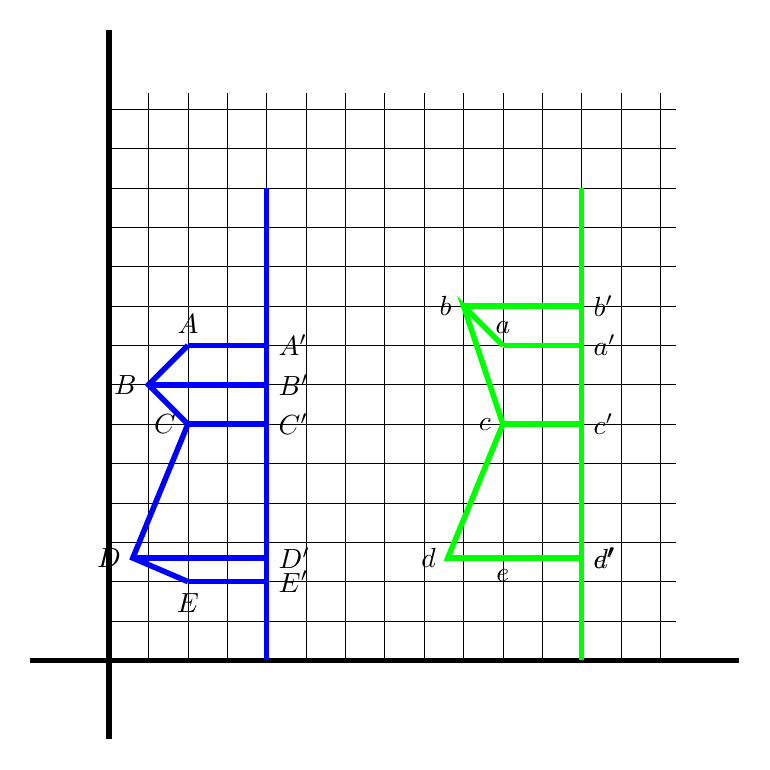
\begin{tikzpicture}[line width=2pt]
\draw (-1,0) -- (8,0);
\draw (0,-1) -- (0,8);
\draw[step=.5cm, very thin] (0,0) grid (7.2,7.2);

\coordinate [label=above:$A$] (A) at (1, 4);
\coordinate [label=left:$B$] (B) at (0.5, 3.5);
\coordinate [label=left:$C$] (C) at (1, 3);
\coordinate [label=left:$D$] (D) at (0.3, 1.3);
\coordinate [label=below:$E$] (E) at (1, 1);

\draw[blue] (A) -- (B) -- (C)  -- (D) -- (E);
\draw[blue] (2, 0) -- (2, 6);

\coordinate [label=right:$A'$] (A') at (2, 4);
\coordinate [label=right:$B'$] (B') at (2, 3.5);
\coordinate [label=right:$C'$] (C') at (2, 3);
\coordinate [label=right:$D'$] (D') at (2, 1.3);
\coordinate [label=right:$E'$] (E') at (2, 1);

\draw[blue] (A) -- (A');
\draw[blue] (B) -- (B');
\draw[blue] (C) -- (C');
\draw[blue] (D) -- (D');
\draw[blue] (E) -- (E');

\coordinate [label=above:$a$] (a) at (5, 4);
\coordinate [label=left:$b$] (b) at (4.5, 4.5);
\coordinate [label=left:$c$] (c) at (5, 3);
\coordinate [label=left:$d$] (d) at (4.3, 1.3);
\coordinate [label=below:$e$] (e) at (5, 1.3);

\draw[green] (a) -- (b) -- (c)  -- (d) -- (e);
\draw[green] (6, 0) -- (6, 6);

\coordinate [label=right:$a'$] (a') at (6, 4);
\coordinate [label=right:$b'$] (b') at (6, 4.5);
\coordinate [label=right:$c'$] (c') at (6, 3);
\coordinate [label=right:$d'$] (d') at (6, 1.3);
\coordinate [label=right:$e'$] (e') at (6, 1.3);

\draw[green] (a) -- (a');
\draw[green] (b) -- (b');
\draw[green] (c) -- (c');
\draw[green] (d) -- (d');
\draw[green] (e) -- (e');
\end{tikzpicture}
\caption{Monotonic polygonal chains}
\label{fig:monotonic_chain}
\end{figure}

\section{表格测试}
\begin{table}[htbp]
  \centering
  \begin{tabular}[htbp]{r|l}
    \toprule
    日期 & 任务 \\
    \midrule
    2011.5 & 完善此份文档 \\
    2011.6 & 完善安装脚本 \\
    \bottomrule
  \end{tabular}
  \caption{表格}
  \label{tab:table1}
\end{table}

\section{源代码高亮测试}

以下是\href{http://acm.zju.edu.cn/onlinejudge/showProblem.do?problemCode=1372}{ZOJ 1372}的解题c++代码:

\begin{lstlisting}[language=c++]
#include <iostream>
#include <string>
using namespace std;
 
const long max_points = 100;
const long infinity = 1000001;
 
int p, r, length, g[max_points][max_points];
bool flag;
 
class vertex
{
public:
    int distance;
    bool visited;
};
 
vertex v[max_points];
 
void initial()
{
    for(int i = 1; i <= p; i++)
        for(int j = 1; j <= p; j++)
            g[i][j] = infinity;
}
 
void prim(int origin)
{
    int temp_min;
    int temp_v = 0;
    int sum = 0;
 
    for(int i = 1; i <= p; i++)
    {
        v[i].distance = g[i][origin];
        v[i].visited = false;
    }
 
    v[origin].distance = 0;
    v[origin].visited = true;
 
    sum++;
 
    while (sum < p)
    {
        temp_min = infinity;
        for(int i = 1; i <= p; i++)
            if(v[i].visited == false && v[i].distance < temp_min)
            {
                temp_min = v[i].distance;
                temp_v = i;
            }
         
        if(temp_min < infinity)
        {
            length += v[temp_v].distance;
            v[temp_v].visited = true;
            sum++;
        }
        else
        {
            flag = true;
            break;
        }
 
        for(int i = 1; i <= p; i++)
        {
            if(v[i].visited == false && v[i].distance > g[i][temp_v])
            {
                v[i].distance = g[i][temp_v];
            }
        }
    }
}
 
int main(int argc, char *argv[])
{
    int a, b, c;
 
    while(cin >> p)
    {
        if(p == 0)
            break;
        cin >> r;
 
        initial();
 
        for(int i = 0; i < r; i++)
        {
            cin >> a >> b >> c;
            if(c < g[a][b])
                g[a][b] = g[b][a] = c;
        }
        length = 0;
        prim(1);
 
        cout << length << endl;
    }
 
    return 0;
} 
\end{lstlisting}

\section{数学公式测试}

著名的爱因斯坦质能方程(\ref{eq:emc2}):

\begin{equation}
  \label{eq:emc2}
  E=mc^2
\end{equation}

计算$f(x)=x^2$的不定积分(\ref{eq:2}):

\begin{equation}
  \label{eq:2}
  \int x^2 dx = \frac{1}{3} x^3
\end{equation}
\section{参考文件测试}
参考文件最好使用bibtex,关于bibtex的使用方法,你可以自行查阅相关文献。

这里是参考文献\cite{c_minigui}

%%%%%%%%%------------------------------------------------------------------------
%%%% 附录

% \appendix    
% \appendixpage
%% 将附录条目添加到contents
% \addappheadtotoc

%%%% 附录结束
%%%%%%%%------------------------------------------------------------------------

%
%%% 加入参考文献支持
%\bibliography{data/main}
%%% 解决目录中没有相应的参考文献的条目问题
%\addcontentsline{toc}{section}{\refname} 
\end{document}
%%%% 正文部分结束
%%%%%%%%------------------------------------------------------------------------
